\documentclass[12pt, reqno]{book}
% \pdfoutput=1



% Packages to open
\usepackage{amsthm, amssymb, amsmath, enumerate, textcomp, cancel}
% \usepackage{fullpage}
\usepackage{verbatim}
\usepackage{graphicx, graphics}
\usepackage{algorithm}
\usepackage{longtable}



\graphicspath{{../Pictures/ProbSolvingPics/}{../Pictures/PlaceValuePics/}{../Pictures/NumberOperationsPics/}{../Pictures/FractionsPics/}{../Pictures/PatternsAlgebraPics/}{../Pictures/DecimalsPics/}{../Pictures/GeometryPics/}{../Pictures/HokuleaPics/}}

% Setup TikZ

\usepackage{tikz}
\usetikzlibrary{arrows}
\tikzstyle{block}=[draw opacity=0.7,line width=1.4cm]

% Hopefully dot packages
\usepackage[all,arc,curve,frame,color]{xy}
\usepackage{subfigure}
\usepackage{url}








% \usepackage{setspace}  % Use command \doublespacing or \onehalfspacing

% Standard Theorem Styles
\newtheorem{thm}{Theorem}[section]
\newtheorem{lem}[thm]{Lemma}
\newtheorem{cor}[thm]{Corollary}
\newtheorem*{cor*}{Corollary}
\newtheorem{prop}[thm]{Proposition}
\newtheorem{obs}[thm]{Observation}
\newtheorem{claim}[thm]{Claim}
\newtheorem*{conjecture*}{Conjecture}
\newtheorem{conjecture}[thm]{Conjecture}
\newtheorem*{thm*}{Theorem}
\newtheorem{ps}{Problem Solving Strategy}

\theoremstyle{remark}
\newtheorem*{question*}{Question}
\newtheorem{question}[thm]{Question}
\newtheorem{answer}[thm]{Answer}
\newtheorem*{remark*}{Remark}
\newtheorem{example}[thm]{Example}
\newtheorem*{thinkpair*}{Think/Pair/Share}



\theoremstyle{definition}
\newtheorem{define}[thm]{Definition}
\newtheorem*{define*}{Definition}
\newtheorem{idea}{Idea}
\newtheorem{problem}{Problem}
\newtheorem{exercise}[thm]{Exercise}
\newtheorem*{problem*}{Problem}
\newtheorem*{sol*}{Solution}


\numberwithin{equation}{section}  % number equations by section

% Standard shortcuts
\newcommand{\LL}{\mathcal{L}}     % Fancy script L
\newcommand{\MM}{\mathcal{M}}  % Fancy script M
\newcommand{\OO}{\mathcal{O}}    % Fancy script O
\newcommand{\FF}{\mathbb{F}}      % Finite field
\newcommand{\ZZ}{\mathbb{Z}}     % Integers
\newcommand{\RR}{\mathbb{R}}     % Reals
\newcommand{\PP}{\mathbb{P}}      % Projective space
\newcommand{\Aff}{\mathbb{A}}      % Affine space
\newcommand{\XX}{\mathcal{X}}      % Model of a variety - script X
\newcommand{\QQ}{\mathbb{Q}}      %Rationals
\newcommand{\CC}{\mathbb{C}}      % Complex Numbers
\newcommand{\mm}{\mathfrak{m}}   % maximal ideal
\newcommand{\pp}{\mathfrak{p}}   % prime ideal
\newcommand{\qq}{\mathfrak{q}}  % another prime ideal
\newcommand{\Gm}{\mathbb{G}_m}  % blackboard bold G for the multiplicative group
\newcommand{\hh}{\mathfrak{h}}  % Upper half plane
\newcommand{\tab}{\hspace{.4cm}} % Tab 



 % Color comments!
\usepackage{xcolor}
% Color comments



%Notes to ourselves
\newcommand{\fellow}[1]{{\color{magenta} \sf $\clubsuit\clubsuit\clubsuit$ Fellow: [#1]}}
\newcommand{\michelle}[1]{{\color{blue} \sf $\clubsuit\clubsuit\clubsuit$ Michelle: [#1]}}


% Some regularly used operator shortcuts
\newcommand{\Hom}{\operatorname{Hom}}
\newcommand{\im}{\operatorname{im}} % Image
\newcommand{\coker}{\operatorname{coker}}  % Cokernel
\newcommand{\Sym}{\operatorname{Sym}}      % Symmetric product
\newcommand{\Spec}{\operatorname{Spec}}
\newcommand{\ord}{\operatorname{ord}}
\newcommand{\Div}{\operatorname{div}}    % Divisor of a rational function
\newcommand{\Gal}{\operatorname{Gal}}  % Galois group
\newcommand{\Gauss}{\operatorname{Gauss}}  % Used for the Gauss point
\newcommand{\supp}{\operatorname{supp}}   % Support
\newcommand{\Pic}{\operatorname{Pic}}        % Picard Groups
\newcommand{\Jac}{\operatorname{Jac}}       % Jacobian Variety
\newcommand{\mult}{\operatorname{mult}}  % multiplicity
\newcommand{\pr}{\operatorname{pr}}     % projection
\newcommand{\sep}[1]{{#1}^{\operatorname{s}}}    % separable closure
\newcommand{\Spf}{\operatorname{Spf}}    % formal spectrum
\newcommand{\Frac}{\operatorname{Frac}}    % Fraction field
\newcommand{\chern}[1]{c_1\left(#1\right)}   % First Chern class
\newcommand{\codim}{\operatorname{codim}}  % codimension
\newcommand{\dist}{\operatorname{dist}}   % distance
\newcommand{\an}[1]{\operatorname{an}}  % analytic space notation
\newcommand{\Aut}{\operatorname{Aut}}   % Automorphism group
\newcommand{\Rat}{\operatorname{Rat}}    % space of rational maps
\newcommand{\PGL}{\operatorname{PGL}}
\newcommand{\PSL}{\operatorname{PSL}}
\newcommand{\alg}[1]{{\overline{#1}}}
\newcommand{\GG}{\mathbb{G}}


% Miscellaneous notational shortcuts
\newcommand{\leftexp}[2]{{\vphantom{#2}}^{#1}{#2}}   % Superscript on the left
\newcommand{\simarrow}{\stackrel{\sim}{\rightarrow}}    % Isomorphic mapping
\newcommand{\ip}[2]{\left\langle #1,#2 \right\rangle} %inner product
\newcommand{\into}{\hookrightarrow}     % Inclusion arrow
\newcommand{\dint}{\int \!\!\! \int}   % double integral
\newcommand{\tth}{^{\operatorname{th}}}
\newcommand{\Berk}{\mathbf{P}}  % Berkovich Projective Space

\newcommand{\Manoa}{M\=anoa}
\newcommand{\Hawaii}{Hawai\kern.05em`\kern.05em\relax i}
\newcommand{\Hokulea}{H\=ok\=ule\kern.05em`\kern.05em\relax a}


% Document Specific Declarations
\newcommand{\id}{\mathrm{id}}
\newcommand{\oo}{\mathfrak{o}}
\DeclareMathOperator{\Per}{Per}
\DeclareMathOperator{\PrePer}{PrePer}
\DeclareMathOperator{\Twist}{Twist}
\DeclareMathOperator{\Ker}{Ker}


%%%%%%%%%%%%%%

\title{Math for Elementary Teachers}




%%%%%%%%%%%%%%


\begin{document}


\maketitle

\tableofcontents


\chapter{Problem Solving}

\fellow{Formatting: can we put things marked ``Problem'' in a box (maybe with some color?) to set it apart?  Same with the Think/Pair/Share (different color?) and Solutions.}

\begin{problem}[ABC]
Draw curves connecting A to A, B to B, and C to C.  Your curves can't cross or even touch each other, and they can't go outside the box.
\begin{center}
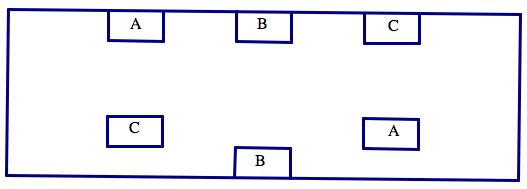
\includegraphics[height=4 cm]{prob1_pic1}
\end{center}
\end{problem}


\begin{thinkpair*}
After you have worked on the problem on your own for a while, talk through your ideas with a partner (even if you haven't solved it).  What did you try?   What makes this problem difficult?  Can you change the problem slightly so that it would be easier to solve?
\end{thinkpair*}

\begin{ps}[Wishful Thinking]
Don't you \emph{\bf wish} the picture in the problem looked more like this one?  Could you solve the problem in that case?
\begin{center}
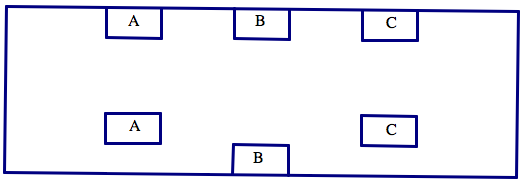
\includegraphics[height=4 cm]{prob1_pic2}
\end{center}
\end{ps}

Can you use a solution to this easier problem to help you solve the original problem?  How?  Think about moving the boxes around once the lines are already drawn.

\fellow{Would be great to have an animation here showing how one solution transforms into the other.  Not sure how hard that would be to create...}

The Common Core State Standards for Mathematics (\url{http://www.corestandards.org/Math/Practice}) identify eight ``Mathematical Practices'' --- the kinds of expertise that all teachers should try to foster in their students, but that go far beyond any particular piece of mathematics content.  They describe what mathematics is really about, and why it is so valuable for students to master.  The very first Mathematical Practice is:

\begin{quote}
``{\bf Make sense of problems and persevere in solving them.}\\
Mathematically proficient students start by explaining to themselves the meaning of a problem and looking for entry points to its solution. They analyze givens, constraints, relationships, and goals. They make conjectures about the form and meaning of the solution and plan a solution pathway rather than simply jumping into a solution attempt. They consider analogous problems, and try special cases and simpler forms of the original problem in order to gain insight into its solution. They monitor and evaluate their progress and change course if necessary.''
\end{quote}

This chapter will help you develop these very important mathematical skills, so that you'll be better prepared to help your future students develop them.


\section{Problem or Exercise?}
The main activity of mathematics is {\bf solving problems}.  But what most people experience in most mathematics classrooms is {\bf practice exercises}.  An exercise is different from a problem.


In a {\bf problem}, you probably don't know at first how to approach solving it.  You 
don't know what mathematical ideas might be used in the solution.  Part of solving a problem is understanding what is being asked, and knowing what a solution should even look like.  Problems often involve false starts, making mistakes, and lots of scratch paper!

In an {\bf exercise}, you are often practicing a skill.  You may have seen a teacher demonstrate a technique, or you may have read a worked example in the book.  You then \emph{practice} on very similar problems, with the goal of mastering that skill.


Note: What is a {\bf problem} for some people may be an {\bf exercise} for other people who have more background knowledge!  For a young student just learning addition, this might be a problem:  
\begin{center}
\emph{Fill in the blank to make a true statement: $\underline{\qquad} + 4 = 7$. }
\end{center}
But for you, that is an exercise!

Both problems and exercises are important in mathematics learning.  But we should never forget that the ultimate goal is to develop more and better skills (through exercises) so that we can solve harder and more interesting problems.  

Learning math is a bit like learning to play a sport.  You can practice lots of skills --- hitting hundreds of forehands in tennis so that you can place them in a particular spot in the court, breaking down strokes into the component pieces in swimming so that each part of the stroke is more efficient, keeping control of the ball while making quick turns in soccer, shooting free throws in basketball, catching high fly balls in baseball, and so on --- but the whole point of the sport is to \emph{play the game}.  You practice the skills so that you're better at playing the game!

The game of math, that's solving problems!

\subsection*{On Your Own}
For each question below, decide if it is a {\bf problem} or an {\bf exercise}.   (You do not need to solve the problems!  Just decide which category it fits for you.)  After you have labeled each one, compare your answers with a partner.

\fellow{Add a mix of exercises.  Use the problems provided here.  Throw in some straightforward computations like adding fractions with unlike denominators, multiplying two-digit numbers, and solving some linear equations.  Make a couple of them ``word problems'' but exercise-y ones like: ``What number is 3 more than 20?''  You can just flip through the book.  Choose about six or seven exercises to go with the problems shows, and intersperse them.}

\begin{enumerate}

\item
 This clock has been broken into three pieces.  If you add the numbers in each piece, the sums are consecutive numbers.  Can you break another clock into a different number of pieces so that the sums are consecutive numbers?  
\begin{center}
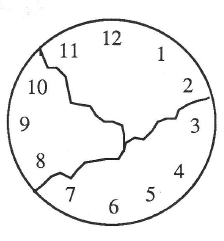
\includegraphics[height=3 cm]{clock}
\end{center}
Assume that each piece has at least two numbers and that no number is damaged (e.g. 12 isn't split into two digits 1 and 2.) 

\fellow{The clock picture is scanned \& stolen from some long-forgotten source.  Any chance we can re-create a version of it?  Even take a picture of a real clock and draw some lines on it?}



\item
Arrange the digits 1--6 into a ``difference triangle'' where each number in the row below is the difference of the two numbers above it.\\

\item
Letters stand for digits 0--9.  In a given problem: the same letter always represents the same digit, and different letters always represent different digits.  There is no relation between problems (so ``A'' in problem one and ``A'' in problem 3 might be different).

\begin{tabular}{c c c c c }
& A & B & C\\
$+$& A & C & B\\\hline
& C & B & A\\
\end{tabular}
\qquad
\begin{tabular}{c c c c c }
& O & N & E\\
$+$& O & N & E\\\hline
& T & W & O\\
\end{tabular}
\qquad
\begin{tabular}{c c c }
&& A \\
&& A \\
$+$&& A \\\hline
&H& A \\
\end{tabular}\\
{\bf Notes:} ``O'' represents the letter O and not the number zero.  Two and three digit numbers never start with 0.  


\item
You have eight coins and a balance scale.  The coins look alike, but one of them is a counterfeit.  The counterfeit coin is lighter than the others.  You may only use the balance scale two times.  How can you find the counterfeit coin?

\fellow{Can we get a picture of a balance scale?  Best if it's one that is in the public sphere or that we create ourselves.}

\item
How many squares are on a standard $8 \times 8$ chess board?


\item
Find the largest eight-digit number made up of the digits 1, 1, 2, 2, 3, 3, 4, and 4 such that the 1s are separated by one digit, the 2s are separated by two digits, the 3s by three digits, and the 4s by four digits.

\end{enumerate}


\section{Problem Solving Strategies}
Think back to the first problem in this chapter.  What did you do to solve it?  Even if you didn't figure it out completely by yourself, you probably worked towards a solution and figured out some things that \emph{didn't} work.   

Unlike exercises, there is never a simple recipe for solving a problem.  You can get better and better at solving problems, both by building up your background knowledge and by simply practicing.  As you solve more problems (and learn how other people solved them), you learn strategies and techniques that can be useful.  But no single strategy works every time. 

\subsection{George Polya}
\fellow{Get a picture of Polya and write a SHORT bio.  You can pull information from the web and from the textbook.  But don't overdo it.}

\subsection{Polya's ``How to Solve it''}
In 1945, Polya published the short book \emph{How to Solve It}, which gave a four-step method for solving mathematical problems:
\begin{enumerate}
\item
First, you have to understand the problem.
\item
After understanding, then make a plan.
\item
Carry out the plan.
\item
Look back on your work. How could it be better?
\end{enumerate}

This is all well and good, but how do you actually {\bf do} these steps?!?!  Steps (1) and (2) are particularly mysterious!  How do you ``make a plan''?  That's where you need some tools in your toolbox, and some experience to draw upon.  

Much has been written since 1945 to explain these steps in more detail, but the truth is that they are more art than science.  This is where math becomes a creative endeavor (and where it becomes so much fun).  We'll articulate some useful problem solving strategies, but no such list will ever be complete.  This is really just a start to help you on your way.  The best way to become a skilled problem solver is to learn the background material well, and then to solve lots of problems!

We have already seen one problem solving strategy, which we called ``Wishful Thinking.''  Don't be afraid to change the problem!  As yourself ``what if'' questions: What if the picture was different?  What if the numbers were simpler?  What if I just made up some numbers?  You need to be sure to go back to the original problem at the end, but wishful thinking can be a powerful strategy for getting started.

This brings us to the most important problem solving strategy of all:
\begin{ps}[Try Something!]
If you're really trying to solve a problem, the whole point is that you don't know what to do right out of the starting gate.  You need to just try something!  Put pencil to paper (or stylus to screen or chalk to board or whatever!) and try something.  This is often an important step in understanding the problem; just mess around with it a bit to understand the situation and figure out what's going on.
\end{ps}

And equally important: If what you tried first doesn't work, try something else!  Play around with the problem until you have a feel for what's going on.



\subsection{Two More Strategies}
\begin{problem}[Payback]
Last week, Alex borrowed money from several of his friends.  He finally got paid at work, so he brought cash to school to pay back his debts.  First he saw Brianna, and he gave her $1/4$ of the money he had brought to school.  Then Alex saw Chris and gave him $1/3$ of what he had left after paying Brianna.  Finally, Alex saw David and gave him $1/2$ of what he had left.  Who got the most money from Alex?
\end{problem}


\begin{thinkpair*}
After you have worked on the problem on your own for a while, talk through your ideas with a partner (even if you haven't solved it).  What did you try?   What did you figure out about the problem, even if you haven't solved it completely.
\end{thinkpair*}


This problem lends itself to two particular strategies.  Did you try either of these as you worked on the problem?  If not, read about the strategy and then try it out before seeing the solution.

\begin{ps}[Draw a Picture]
Some problems are obviously about a geometric situation, and it's clear you want to draw a picture and mark down all of the given information before you try to solve it.  But even for a problem that isn't geometric, like this one, thinking visually can help!  Can you represent something in the situation by a picture?  
\end{ps}

Draw a square to represent all of Alex's money.  Then shade $1/4$ of the square --- that's what he gave away to Brianna.  How can the picture help you finish the problem?

After you have worked on the problem yourself using this strategy (or if you're totally stuck), you can watch someone else's solution:
\fellow{Add an animation of the solution described as shown in Monique's book?}


\begin{ps}[Make Up Numbers]
Part of what makes this problem difficult is that it's about money, but there are no numbers given.  That means the numbers must not be important.  So just make them up!  
\end{ps}

You can  work forwards: Assume Alex had some specific amount of money when she showed up at school, say \$100.  Then figure out how much he gives to each person.  Or you can work backwards: suppose he has some specific amount left at the end, like \$10.  Since he gave Chris half of what he had left, that means he had \$20 before running into Chris.   Now, work backwards and figure out how much each person got.

Watch the solution only after you tried this strategy for yourself:
\fellow{Add an animation of the solution described as shown in Monique's book?}

If you use the ``Make Up Numbers'' strategy, it's really important to remember what the original problem was asking!  You don't want to answer something like ``Everyone got \$10.''  That's not true in the original problem; that's an artifact of the numbers you made up.  So after you work everything out, be sure to re-read the problem and {\bf answer what was asked}!



\subsection{Four More Strategies}
\begin{problem}[Squares on a Chess Board]\label{prob:chessboard}
How many squares are on a standard $8 \times 8$ chess board?  (The answer is \emph{not} 64!  It's a lot bigger!)
\end{problem}

Remember Polya's first step is to understand the problem.  If you're not sure what's being asked, or why the answer is not just 64, be sure to ask someone!


\begin{thinkpair*}
After you have worked on the problem on your own for a while, talk through your ideas with a partner (even if you haven't solved it).  What did you try?   What did you figure out about the problem, even if you haven't solved it completely.
\end{thinkpair*}


It's pretty clear that you want to draw a picture for this problem, but even with the picture it can be hard to know if you've found the correct answer.  The numbers get big, and it can be hard to keep track of your work.  Your goal at the end is to be \emph{absolutely positive} that you found the right answer.  You should never ask the teacher, ``Is this right?''  Instead, you should declare, ``Here's my answer, and here's why I know it's correct!''


\begin{ps}[Try a Simpler Problem]
 Polya suggested this strategy: ``If you can't solve a problem, then there is an easier problem you can solve: find it.''  He also said: ``If you cannot solve the proposed problem, try to solve first some related problem. Could you imagine a more accessible related problem?''  In this case, an $8 \times 8$ checkerboard is pretty big.  Can you solve the problem for smaller boards?  Like $1 \times 1$?  $2 \times 2$?  $3 \times 3$?
\end{ps}

Of course the ultimate goal is to solve the original problem.  But working with smaller boards might give you some insight and help you devise your plan (that's Polya's step (2)).


\begin{ps}[Work Systematically]
If you're working on simpler problems, it's useful to keep track of what you've figured out and what changes as the problem gets more complicated. 
\end{ps}

 For example, in this problem you might keep track of how many $1\times 1$ squares are on each board, how many $2\times2$ squares on are each board, how many $3 \times 3$ squares are on each board, and so on.  You could keep track of the information in a table:
 
 \begin{tabular}{ |c| | c| c| c| c| c|  }\hline
 size of board &  $1 \times 1 $ squares &  $2 \times 2 $ squares &  $3 \times 3 $ squares &  $4 \times 4 $ squares & \dots \\\hline\hline
 $1 \times 1 $ & 1 & 0 & 0 & 0 & \dots\\
 \hline
 $2 \times 2 $ & 4 & 1 & 0 & 0 & \dots\\
 \hline
  $3 \times 3 $ &   &   &   &   & \dots\\
  \hline
  \vdots &  & & & & \\
  \hline
\end{tabular}


\begin{ps}[Use Manipulatives to Help You Investigate]
Sometimes even drawing a picture may not be enough to help you investigate a problem.  Having actual materials that you move around can sometimes help a lot!
\end{ps}

For example, in this problem it can be difficult to keep track of which squares you've already counted.  You might want to cut out $1 \times 1$ squares, $2 \times 2$ squares, $3 \times 3$ squares, and so on.  You can actually move the smaller squares across the checkerboard in a systematic way, making sure that you count everything once and don't count anything twice.

\fellow{Make a video showing how to do this on a $5 \times 5$ board, using cutouts of a $2 \times 2$ and / or a $3 \times 3$?}


\begin{ps}[Look for and Explain Patterns]
Sometimes the numbers in a problem are so big, there's no way you will actually count everything up by hand.  For example, if the problem in this section were about a $100 \times 100$ chess board, you wouldn't want to go through counting all the squares by hand!  It would be much more appealing to find a pattern in the smaller boards and then extend that pattern to solve the problem for a $100 \times 100$ chess board just with a calculation.
\end{ps}


\begin{thinkpair*}
If you haven't done so already, extend the Table above all the way to an $8\times 8$ chess board, filling in all the rows and columns.  Use your table to find the total number of squares in an $8 \times 8$ chess board.  Then:
\begin{itemize}
\item
Describe all of the patterns you see in the table.  
\item
Can you \emph{explain} and \emph{justify} any of the patterns you see?  How can you be sure they will continue?
\item
What calculation would you do to find the total number of squares on a $100 \times 100$ chess board?
\end{itemize}
\end{thinkpair*}

(We'll come back to this question in Section~\ref{sec:BewarePatterns}.  So if you're not sure right now how to explain and justify the patterns you found, that's OK.)



\subsection{Two More Strategies}
\begin{problem}[Broken Clock]\label{prob:BrokenClock}
 This clock has been broken into three pieces.  If you add the numbers in each piece, the sums are consecutive numbers.  Can you break another clock into a different number of pieces so that the sums are consecutive numbers?  
\begin{center}
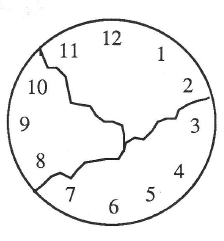
\includegraphics[height=3 cm]{clock}
\end{center}
Assume that each piece has at least two numbers and that no number is damaged (e.g. 12 isn't split into two digits 1 and 2.) 
\end{problem}


\fellow{Replace clock picture as before.}

Remember that your first step is to understand the problem.  Work out what's going on here.  What are the sums of the numbers on each piece?  Are they consecutive?  (What does that mean?)

\begin{thinkpair*}
After you have worked on the problem on your own for a while, talk through your ideas with a partner (even if you haven't solved it).  What did you try?   What progress have you made?
\end{thinkpair*}


\begin{ps}[Find the Math, Remove the Context]
Sometimes the problem has a lot of details in it that are unimportant, or at least unimportant for getting started.  The goal is to find the underlying math problem, then come back to the original question and see if you can solve it using the math.
\end{ps}

In this case, worrying about the clock and exactly how the pieces break is less important than worrying about finding consecutive numbers that sum to the correct total.  Ask yourself: 
\begin{itemize}
\item
What is the sum of all the numbers on the clock's face?  
\item
Can I find two consecutive numbers that give the correct sum?  Or four consecutive numbers?  Or some other amount?
\item
How do I know when I'm done?  When should I stop looking?
\end{itemize}

Of course, solving the question about consecutive numbers is not the same as solving the original problem.  You have to go back and see if the clock can actually break apart so that each piece gives you one of those consecutive numbers.  Maybe you can solve the math problem, but it doesn't translate into solving the clock problem.

\begin{ps}[Check Your Assumptions]
When solving problems, it's easy to limit your thinking by adding extra assumptions that aren't in the problem.  Be sure you ask yourself: Am I constraining my thinking too much?
\end{ps}

In the clock problem, because the first solution has the clock broken \emph{radially} (all three pieces meet at the center, so it looks like slicing a pie), many people assume that's how the clock must break.  But the problem doesn't require the clock to break radially.  It might break into pieces like this:

\fellow{Add a picture of a clock broken into pieces with the breaks going across, not radial.  For example, three pieces: $\{11, 12, 1, 2\}$, $\{10,9, 3, 4, 5\}$, and $\{6,7,8\}$.}


Were you assuming the clock would break in a specific way?  Try to solve the problem now, if you haven't already.  


\section{Beware of Patterns!}\label{sec:BewarePatterns}

The ``Look for Patterns'' strategy can be particularly appealing, but you have to be careful!  Don't forget the {\bf ``and Explain''} part of the strategy.  Not all patterns are obvious, and not all of them will continue.

\begin{problem}[Dots on a Circle]
Start with a circle.  
\begin{center}

\includegraphics[height=3 cm]{circle}
\end{center}
If I put two dots on the circle and connect them, the line divides the circle into two pieces.
\begin{center}
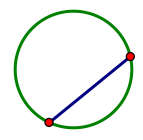
\includegraphics[height=3 cm]{twodots}
\end{center}
If I put three dots on the circle and connect each pair of dots, the lines divides the circle into four pieces.
\begin{center}
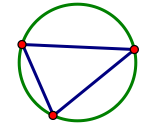
\includegraphics[height=3 cm]{threedots}
\end{center}
Suppose you put one hundred dots on a circle and connect each pair of dots.  How many pieces will you get? 
\end{problem}

\begin{thinkpair*}
After you have worked on the problem on your own for a while, talk through your ideas with a partner (even if you haven't solved it).  What strategies did you try?   What did you figure out?  What questions do you still have?
\end{thinkpair*}


The natural way to work on this problem is to use smaller numbers of dots and look for a pattern, right?  If you haven't already, try it.  How many pieces when you have four dots?  Five dots?   How would you describe the pattern?

Now try six dots.  You'll want to draw a \emph{big} circle and space out the six dots to make your counting easier.  Then carefully count up how many pieces you get.  It's probably a good idea to work with a partner so you can check each other's work.  Make sure you count every piece once and don't count any piece twice.  How can you be sure that you do that?

Were you surprised?  For the first several steps, it  \emph{seems} to be the case that when you add a dot you double the number of pieces.  But that would mean that for six dots, you should get 32 pieces, and you only get 31!  The pattern simply doesn't hold up.


Mathematicians love looking for patterns and finding them.  We get excited by patterns.   But we are also very skeptical of patterns!  If we can't explain \emph{why} a pattern would occur, then we aren't willing to just believe it!  

For example, if my number pattern starts out 
\[
2, 4, 8, \dots
\]
I can find \emph{lots} of ways to continue the pattern, each of which makes sense in some contexts.  Here are some possibilities:
\begin{itemize}
\item
$2, 4, 8, 2, 4, 8, 2, 4, 8, 2, 4, 8, \dots$. \\
This is a a repeating pattern, cycling through the numbers $2, 4, 8$ and then starting over with $2$.\\

\item
$2, 4, 8, 32, 256, 8192,  \dots$. \\
To get the next number, multiply the previous two numbers together.\\

\item
$2, 4, 8, 16, 32, 64, 128, 256, 512, 1024,  \dots$. \\

\item
$2, 4, 8, 14, 22, 32, 44, 58, 74  \dots$. \\

\end{itemize}


\begin{thinkpair*}
Work on your own and then share your ideas with a partner:
\begin{enumerate}
\item
For the last two patterns above, describe in words how the number sequence is being created.  
\item
Find at least two other ways to continue the sequence $2, 4, 8, \dots$ that looks different from all the ones you've seen so far.  Write your rule in words, and write the next five terms of the number sequence.
\end{enumerate}
\end{thinkpair*}

So how can you be sure your pattern fits the problem?  You have to tie them together!  Remember the ``Squares on a Chess Board'' problem?  You might have noticed a pattern like this one:

If the chess board has 5 squares on a side, then there are
\begin{itemize}
\item
$5 \times 5 =25$ squares of size $1 \times 1$.
\item
$4 \times 4 = 16$ squares of size $2 \times 2$.
\item
$3 \times 3 =9$ squares of side $3 \times 3$.
\item 
$2 \times 2 = 4$ squares of size $4 \times 4$.
\item
$1 \times 1 = 1$ squares of size $5 \times 5$.
\end{itemize}
So there are a total of
\[
1^2 + 2^2 + 3^2 + 4^2 + 5^2 = 55
\]
squares on a $5 \times 5$ chess board.

You can probably guess how to continue the pattern to any size board, but  how can you be \emph{absolutely sure} the pattern continues in this way?  What if this is like ``Dots on a Circle,'' and the obvious pattern breaks down after a few steps? You have to tie the pattern to the problem, so that it's clear why the pattern \emph{must} continue in that way.

The first step in explaining a pattern is writing it down clearly.  This brings us to another problem solving strategy.

\begin{ps}[Use a Variable!]
One of the most powerful tools we have   is the use of a \emph{variable}.  If you find yourself doing calculations on things like ``the number of squares,'' or ``the number of dots,'' give those quantities a name!  They become much easier to work with.
\end{ps}

\begin{thinkpair*}
For now, just work on \emph{describing} the pattern with variables.  
\begin{itemize}
\item
Stick with a $5 \times 5 $ chess board for now, and consider a small square of size $k \times k$.  Describe the pattern: How many squares of size $k \times k$ fit on a chess board of size $5\times 5$?
\item
What if the chess board is bigger?  Based on the pattern above,  how many squares of size $k \times k$ \emph{should} fit on a chess board of size $10 \times 10$?
\item
What if you don't know how big the chess board is?  Based on the pattern above,  how many squares of size $k \times k$ \emph{should} fit on a chess board of size $n \times n$?
\end{itemize}
\end{thinkpair*}

Now comes the tough part: \emph{explaining} the pattern.  Let's focus on an $8 \times 8$ board.  Since it measures $8$ squares on each side, we can see that we get $8 \times 8 = 64$ squares of size $1 \times 1$.  And since there's just a single board, we get just one square of size $8 \times 8$.  But what about all the sizes in-between?

\fellow{Insert video showing why the count for $2 \times 2$ squares should be $7 \times 7  = 49$.  Model it on the general solution below.}

\begin{thinkpair*}
Using the video as a model, work with a partner to carefully explain why the number of $3 \times 3$ squares will be $6 \times 6 = 36$, and why the number of $4 \times 4$ squares will be $4 \times 4 = 16$.
\end{thinkpair*} 

Here's what a final justification might look like:  

\begin{sol*}[Chess Board Pattern]
Let $n$ be the side of the chess board and let $k$ be the side of the square.  If the square is going to fit on the chess board at all, it must be true that $k \leq n$.  Otherwise, the square is too big.

If I put the $k \times k$ square in the upper left corner of the chess board, it takes up $k$ spaces across and there are $(n-k)$ spaces to the right of it.  So I can slide the $k \times k$ square to the right $(n-k)$ times, until it hits the top right corner of the chess board.  The square is in $(n-k+1)$ different positions, counting the starting position.

If I move the $k \times k$ square back to the upper left corner, I can shift it down one row and repeat the whole process again.  Since there are $(n-k)$ rows below the square, I can shift it down $(n-k)$ times until it hits the bottom row.  This makes $(n-k+1)$ total rows that the square moves across, counting the top row.

So there are $(n-k+1)$ rows with $(n-k+1)$ squares in each row.  That makes $(n-k+1)^2$ total squares.  
\end{sol*}

Once we're sure the pattern continues, we can use it to solve the problem.  So go ahead!  
\begin{itemize}
\item
How many squares on a $10 \times 10$ chess board?    
\item
What calculation would you do to solve that problem for a $100 \times 100$ chess board?
\end{itemize}


There \emph{is} a number pattern that describes the number of pieces you get from the ``Dots on a Circle'' problem.  If you want to solve the problem, go for it!  Think about all of your problem solving strategies.  But be sure that when you find a pattern, you can explain \emph{why} it's the right pattern for this problem, and not just another pattern that seems to work but might not continue.


\section{Problem Bank}\label{sec:ProblemBank}
You have several problem solving strategies to work with.  Here are the ones we've described in this Section (and you probably came up with even more of your own strategies as you worked on problems).
\begin{enumerate}
\item
Wishful Thinking.
\item
Try Something!
\item
Draw a Picture.
\item
Make up Numbers.
\item
Try a Simpler Problem.
\item
Work Systematically.
\item
Use Manipulatives to Help You Investigate.
\item
Look for and Explain Patterns.
\item
Find the Math, Remove the Context.
\item
Check Your Assumptions.
\item
Use a Variable.
\end{enumerate}

Try your hand at some of these problems, keeping these strategies in mind.  If you're stuck on a problem, come back to this list and ask yourself which of the strategies might help you make some progress.


\fellow{If you have any favorite problems that don't have a lot of mathematical prerequisites --- this is the first chapter! --- throw them in!  The more the merrier!}



\begin{problem}
You have eight coins and a balance scale.  The coins look alike, but one of them is a counterfeit.  The counterfeit coin is lighter than the others.  You may only use the balance scale two times.  How can you find the counterfeit coin?

\fellow{Balance scale picture?}
\end{problem}



\begin{problem}
You have five coins, no two of which weigh the same.  In seven weighings on a balance scale, can you put the coins in order from lightest to heaviest?  That is, can you determine which  coin is the lightest, next lightest, \dots, heaviest.  
\end{problem}

\begin{problem}
You have ten bags of coins.  Nine of the bags contain good coins weighing one ounce each.  One bag contains counterfeit coins weighing 1.1 ounces each.  You have a regular (digital) scale, not a balance scale.  The scale is correct to one-tenth of an ounce.  In one weighing, can you determine which bag contains the bad coins?
\end{problem}

\begin{problem}
Suppose you have a balance scale.  You have three different weights, and you are able to weigh every whole number from 1 gram to 13 grams using just those three weights.  What are the three weights?  
\end{problem}



\begin{problem}
There are a bunch of coins on a table in front of you.  Your friend tells you how many of the coins are heads-up.  You are blindfolded and can't see a thing, but you can move the coins around, and you can flip them over.  However, you can't tell just by feeling them if the coins are showing heads or tails.  Your job: separate the coins into two piles so that the same number of heads are showing in each pile.
\end{problem}


\begin{problem}
The digital root of a number is the number obtained by adding the digits of the number.  If the answer is not a one-digit number, add those digits.  Continue until a one-digit sum is reached.  This one digit is the digital root of the number.  For example, the digital root of 98 is 8, since 
$$
9+8 = 17 \quad \text{and} \quad 1+7 = 8.
$$
Record the digital roots of the first $30$ integers and find as many  patterns as you can.  Can you explain any of the patterns?  Can you predict the digital root of a number without computing it? 
\end{problem}

\begin{problem}
If this lattice were continued, what number would be directly to the right of $98$?
\begin{center}
\begin{tabular}{c c c c c c c c c c c}
& 3 &  & 6 &  & 9 &  & 12 & &\ldots \\
1 & 2& 4&  5 & 7 & 8 & 10 & 11 & 13 & \ldots  \\
\end{tabular}
\end{center}

\end{problem}





\begin{problem}
Arrange the digits $0$ through $9$ so that the first digit is divisible by $1$, the first two digits are divisible by $2$, the first three digits are divisible by $3$, and continuing until you have the first $9$ digits divisible by $9$ and the whole $10$-digit number divisible by~$10$.
\end{problem}

\begin{problem}
There are 25 students and one teacher in class.  After an exam, everyone high-fives everyone else to celebrate how well they did.  How many high-fives were there?
\end{problem}




\begin{problem}
In cleaning out your old desk, you find a whole bunch of $3$\textcent\ and $7$\textcent\ stamps.  Can you make exactly $11$\textcent\ of postage?  Can you make exactly $19$\textcent\ of postage?  What is the largest amount of postage you cannot make?  
\end{problem}


\begin{problem}
Find the largest eight-digit number made up of the digits 1, 1, 2, 2, 3, 3, 4, and 4 such that the 1s are separated by one digit, the 2s are separated by two digits, the 3s by three digits, and the 4s by four digits.
\end{problem}



\begin{problem}
Kami has ten pockets and 44 dollar bills.  She wants to have a different amount of money in each pocket.  Can she do it?
\end{problem}


\begin{problem}
How many triangles are in this picture?
\begin{center}
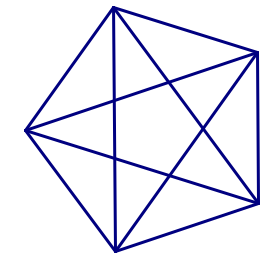
\includegraphics[height=3 cm]{pent_tris}
\end{center}


\end{problem}

\begin{problem}
Arrange the digits 1--6 into a ``difference triangle'' where each number in the row below is the difference of the two numbers above it.\\
{\bf Example:} This is a difference triangle, but it doesn't work because it uses 1 twice and doesn't have a 6:

\begin{center}
\begin{tabular}{c c c c c}
4 && 5 && 3 \\
 & 1 && 2\\
 &&1 \\
 \end{tabular}
 \end{center}
\end{problem}


\begin{problem}
Certain pipes are sold in lengths of 6 inch, 8 inch, and 10 inches.  How many different lengths can you form by attaching three sections of pipe together?
\end{problem}

\begin{problem}
Place the digits 1, 2, 3, 4, 5, 6 in the circles so that the sum on each side of the triangle is 12.  Each circle gets one digit, and each digit is used exactly once.
\begin{center}
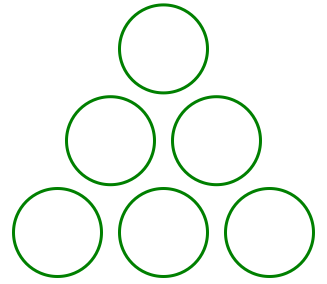
\includegraphics[height=3 cm]{circle_pyr}
\end{center}

\end{problem}


\begin{problem}
Find a way to cut a circular pizza into 11 pieces using just four straight cuts.
\end{problem}



\section{Careful use of Language in Mathematics}
This section might seem like a bit of a sidetrack from the idea of problem solving, but in fact it's not.  Mathematics is a social endeavor.  We don't just solve problems and then put them aside.  Problem solving has (at least) three components:
\begin{enumerate}
\item
Solving the problem.  This involves lots of scratch paper and careful thinking.
\item
Convincing \emph{yourself} that your solution is complete and correct.  This involves a lot of self-check and asking yourself questions.
\item
Convincing \emph{someone else} that your solution is complete and correct.  This usually involves writing the problem up carefully or explaining your work in a presentation.
\end{enumerate}

If you're not able to do that last step, then you haven't really solved the problem.  We'll talk more about how to write up a solution in the next section.  Before we do that, we have to think about how mathematicians use language (which is, it turns out, a bit different from how language is used in the rest of life).

\subsection{Mathematical Statements}

\begin{define}
A {\bf mathematical statement} is a complete sentence that is either true or false.
\end{define}

So a ``statement'' in mathematics cannot be a question, a command, or a matter of opinion.  It is a complete, grammatically correct sentence (with a subject, verb, and usually an object).  It's important that the statement is either true or false, though you may not know which!  (Part of the work of a mathematician is figuring out which sentences are true and which are false.

\begin{thinkpair*}
For each English sentence below, decide if it is a mathematical statement or not.  If it is, is the statement true or false (or are you unsure)?  If it is not, in what way does it fail?

\begin{enumerate}
\item
I like the color blue.
\item
$60$ is an even number.
\item
Is your dog friendly?
\item
Honolulu is the capital of Hawaii.
\item
This sentence is false.
\item
Roses are red.
\item
UH Manoa is the best college in the world.
\item
$1/2 = 2/4$.
\item
Go to bed.
\item
There are a total of 204 squares on an $8 \times 8$ chess board.
\end{enumerate}

Now, work with a partner.  Write three mathematical statements and three English sentences that fail to be mathematical statements.
\end{thinkpair*}

Notice that ``$1/2 = 2/4$'' is a perfectly good mathematical statement.  It doesn't look like an English sentence, but read it out loud.  The subject is ``$1/2$.'' The verb is ``equals.''  And the object is ``$2/4$.''  This is a very good test when you write mathematics: try to read it out loud.  Even the equations should read naturally, like English sentences. 

Statement (5) is different from the others.  It is called a \emph{paradox}: a statement that is self-contradictory.  If it is true, then we conclude that it is false.  (Why?)  If it is false, then we conclude that it is true.  (Why?)  Paradoxes are no good as mathematical statements.  

\subsection{Precision}
When we use words in an everyday situation, we often rely on context and shared understanding.
The American Academy of Dermatology has this sentence on their web page: 
\begin{center}
``One American dies of melanoma every hour.''
\end{center}

Taken literally (as a mathematician would), this statement makes an absurd claim:  There is one person in America who keeps dying over and over.  In fact, he dies \emph{every single hour}.

A more precise statement would be this:
``Every hour, someone in America dies of melanoma.''

\begin{thinkpair*}
Compare the two sentences:
\begin{itemize}
\item
``One American dies of melanoma every hour.''
\item
``Every hour, someone in America dies of melanoma.''
\end{itemize}
What is the (subtle) difference?  Why does that small difference change the meaning so dramatically?

\end{thinkpair*}

 If we're working on mathematical problem, we need to work with clear and correct statements.  We cannot make assumptions about context or shared understanding.  We have to say exactly what we mean.

\subsection*{On Your Own}
Work on the exercises below to reinforce the idea of using precise language.
\begin{enumerate}
\item
Consider this ambiguous sentence:
\begin{center}
\emph{``The man saw
the woman with a telescope.''} 
\end{center}
Find two unambiguous (but natural sounding) sentences equivalent to the sentence above, one in which the
 man has the telescope, and one in which  the woman
has the telescope.
 
 
 \item
Here are three ambiguous newspaper headlines.  For each one, rewrite it in a way that avoids the unintended second meaning.  But keep it short and pithy, like a newspaper headline should be.

\begin{enumerate}
\item
Sisters reunited after 10 years in checkout line of Longs Drugs.
\item
Large hole appears on H-1.  County authorities are looking into it.
\item
Governor Abercrombie says bus passengers should be belted.

\end{enumerate}


 \item
This hospital notice says exactly the opposite of what it means to say.
 \begin{center}
\emph{``No head injury is too trivial to ignore.''} 
\end{center}
Rewrite the sentence so it would still fit on the sign, but would convey its intended meaning.



\end{enumerate}


\subsection{And / or}
Consider this sentence 
\begin{center}
\emph{``After work, I will go to the beach or I will do my grocery shopping.''}
\end{center}
In everyday English, that probably means that if I go to the beach, I will not go shopping.  I will do one or the other, but not both activities.  This is called an ``exclusive or.''

We can usually tell from context whether a speaker means ``either one or the other or both,'' or whether he means ``either one or the other but not both.''  (Some people use the awkward phrase ``and/or'' to describe the first option.)  

Remember that in mathematical communication, though, we have to be very precise.  We cannot rely on context or assumptions about what is implied or understood.
\begin{define}
In mathematics, the word ``or'' \emph{always means} ``either one or the other or both.''
\end{define}

\begin{thinkpair*}
For each sentence below:
\begin{itemize}
\item
Decide if the choice $x = 3$ makes the statement true or false.  
\item
Choose a different value of $x$ that makes the statement true (or say why that's not possible).
\item
Choose a different value of $x$ that makes the statement false (or say why that's not possible).
\end{itemize}

\begin{enumerate}
\item
$x$ is odd or $x$ is even.
\item
$x$ is odd and $x$ is even.
\item
$x$ is prime or $x$ is negative.
\item
$x >5$ or $x < 5$.
\item
$x >5$ and $x < 5$.
\item
$x + 1 = 7$ or $x - 1 = 7$.
\item
$x \cdot 1 = x$ or $x \cdot 0 = x$.
\item
$x \cdot 1 = x$ and $x \cdot 0 = x$.
\end{enumerate}
\end{thinkpair*}



\subsection{Quantifiers}
\begin{problem}[All About the Benjamins]
You are handed an envelope filled with money, and you are told ``Every bill in this envelope is a \$100 bill.''
\begin{itemize}
\item
What would convince you \emph{beyond any doubt} that the sentence is true?  How could you convince someone else that the sentence is true?

\item 
What would convince you \emph{beyond any doubt} that the sentence is false?  How could you convince someone else that the sentence is false?
\end{itemize}

Suppose you were given a different sentence: ``There is a \$100 bill in this envelope.''
\begin{itemize}
\item
What would convince you \emph{beyond any doubt} that the sentence is true?  How could you convince someone else that the sentence is true?

\item 
What would convince you \emph{beyond any doubt} that the sentence is false?  How could you convince someone else that the sentence is false?
\end{itemize}
\end{problem}

\begin{thinkpair*}
After you have thought about the problem on your own for a while, talk through your ideas with a partner.  What is the difference between the two sentences?  How does that difference affect your method to decide if the statement is true or false?
\end{thinkpair*}

Some mathematical statements have this form:
\begin{itemize}
\item
``Every time\dots''
\item
``For all numbers\dots''
\item
``For every choice\dots''
\item
``It's always true that\dots''
\end{itemize} 
These are \emph{universal statements}.  Such statements claim that something is always true, no matter what.  

\begin{itemize}
\item
To prove a \emph{universal statement} is false, you must find an example where it fails.  This is called a {\bf counterexample} to the statement.
\item
To prove a \emph{universal statement} is true, you must either check every single case, or you must find a {\bf logical reason} why it would be true.  (Sometimes the first option is impossible, because there might be infinitely many cases to check.  You would never finish!)
\end{itemize}


Some mathematical statements have this form:
\begin{itemize}
\item
``Sometimes\dots''
\item
``There is some number\dots''
\item
``For some choice\dots''
\item
``At least once\dots''
\end{itemize} 
These are \emph{existential statements}.  Such statements claim there is some example where the statement  is  true, but it may not always be true.  

\begin{itemize}
\item
To prove an \emph{existential statement} is true, you may just find the example where it works.  
\item
To prove an \emph{existential statement} is false, you must either show it fails in every single case, or you must find a {\bf logical reason} why it can't be true.  (Sometimes the first option is impossible!)
\end{itemize}



\begin{thinkpair*}
For each statement below, do the following:
\begin{itemize}
\item
Decide if it is a \emph{universal statement} or an \emph{existential statement}.  (This can be tricky because in some statements the quantifier is ``hidden'' in the meaning of the words.)
\item
Decide if the statement is true or false, and do your best to justify your decision.
\end{itemize}

\begin{enumerate}
\item
Every odd number is prime.
\item
Every prime number is odd.
\item
For all positive numbers $x$, $x^3 > x$.
\item
There is some number $x$ such that $x^3 = x$.
\item
The points $(-1,1)$, $(2,1)$, and $(3,0)$ all lie on the same line.
\item
Addition (of real numbers) is commutative.
\item
Division (of real numbers) is commutative.
\end{enumerate}

Look back over your work.  you will probably find that some of your arguments are sound and convincing while others are less so.  In some cases you may ``know'' the answer but be unable to justify it.  That's okay for now!  Divide your answers into four categories:

\bigskip

\begin{enumerate}[(a)]
\item
I am confident that the justification I gave is good.
\item
I am not confident in the justification I gave.
\item
I am confident that the justification I gave is \emph{not} good, or I could not give a justification.
\item
I could not decide if the statement was true or false.
\end{enumerate}


\end{thinkpair*}

\subsection{Conditional statements}
\begin{problem}[Card Logic]
These cards are on a table.
\begin{center}
\includegraphics[height=3 cm]{cards}
\end{center}
Your friend claims: ``If a card has a vowel on one side, then it has an even number on the other side.'' Which cards \emph{must} you flip over to  be certain that your friend is telling the truth?
\end{problem}


\fellow{Picture is stolen from a long-forgotten source.  Can we re-create it so it's not any kind of copyright violation?}


\begin{thinkpair*}
After you have thought about the problem on your own for a while, discuss your ideas with a partner.  Do you agree on which cards you must check?   Try to come to agreement on an answer you both believe.
\end{thinkpair*}

Here is another very similar problem, yet people seem to have an easier time solving this one:


\begin{problem}[IDs at a Party]
You are in charge of a party where there are young people. Some are drinking alcohol, others soft
drinks. Some are old enough to drink alcohol legally, others are under age. You are responsible for
ensuring that the drinking laws are not broken, so you have asked each person to put his or her
photo ID on the table. At one table, there are four young people:
\begin{itemize}
\item
One person has a beer, another has a
Coke, but their IDs happen to be face down so you cannot see their ages. 
\item
You can, however, see the
IDs of the other two people. One is under the drinking age, the other is above it. Unfortunately,
you are not sure if they are drinking Seven-up or vodka and tonic. 
\end{itemize}
Which IDs and/or drinks do you
need to check to make sure that no one is breaking the law?
\end{problem}

\begin{thinkpair*}
After you have thought about the problem on your own for a while, discuss your ideas with a partner.  Do you agree on which cards you must check?   Compare these two problems.
Which question is easier and why?
\end{thinkpair*}

\begin{define}
A {\bf conditional statement} can be written in the form
\begin{center}
If $\underbrace{\quad \text{\emph{some statement}} \quad}_{\text{hypothesis}}$ then $\underbrace{\quad \text{\emph{some statement}}  \quad}_{\text{conclusion}}$.
\end{center}
\end{define}

\begin{thinkpair*}
 These are each conditional statements, though they are not all stated in ``if/then'' form.  Identify the hypothesis of each statement.  (You may want to rewrite the sentence as an equivalent ``if/then'' statement.)
 \vspace{.2in}

 \begin{enumerate}
\item 
If the tomatoes are red, then they are ready to eat.\\
The tomatoes are red. \qquad / \qquad The tomatoes are ready to eat.


\item
An integer $n$ is even if it is a multiple of 2.\\
$n$ is even. \qquad / \qquad $n$ is a multiple of 2.



\item
If $2^n - 1$ is prime, then $n$ is prime.\\
$n$ is prime. \qquad / \qquad $2^n-1$ is prime.



\item
The team wins when JJ plays.\\
The team wins. \qquad / \qquad JJ plays.


\end{enumerate}
\end{thinkpair*}

Remember that a mathematical statement must have a definite truth value.  It's either true or false, with no gray area (even though we may not be sure which is the case).  How can you tell if a conditional statement is true or false?  Surely, it depends on whether the \emph{hypothesis} and the \emph{conclusion} are true or false.  But how, exactly, can you decide?

The key is to think of a conditional statement like a promise, and ask yourself: under what condition(s) will I have broken my promise?

\begin{example}
Here is a conditional statement:
\begin{center}
``If $\underbrace{\text{I win the lottery}}_{\text{hypothesis}}$, then $\underbrace{\text{I'll give  each of my students \$1,000}}_{\text{conclusion}}$.''
\end{center}

There are four things that can happen:
\begin{description}
\item[True hypothesis, true conclusion] I do win the lottery, and I do give everyone in class \$1,000.   I kept my promise, so the conditional statement is TRUE.
\item[True hypothesis, false conclusion] I do win the lottery, but I decide {\bf not to} give everyone in class \$1,000.   I broke my promise, so the conditional statement is FALSE.
\item[False hypothesis, true conclusion] I don't win the lottery, but I'm exceedingly generous, so I go ahead and give everyone in class \$1,000.  I didn't break my promise!  (Do you see why?)  So the conditional statement is TRUE.
\item[False hypothesis, false conclusion] I don't win the lottery,  so I don't give everyone in class \$1,000.  I didn't break my promise!  (Do you see why?)  So the conditional statement is TRUE.
\end{description}
\end{example}

What can we conclude from this?  {\bf A conditional statement is false only when the hypothesis is true and the conclusion is false.}  In every other instance, the promise (as it were) has not been broken.  If the statement is not false, it must be true.

\begin{example}
Here's another conditional statement:
\begin{center}
``If you live in Honolulu, then you live in Hawaii.''
\end{center}
Is this statement true or false?  It seems like it should depend on who the pronoun ``you'' refers to, and whether that person lives in Honolulu or not.  Let's think it through:
\begin{itemize}
\item
Sookim lives in Honolulu, so the hypothesis is true.  Since Honolulu is in Hawaii, she does live in Hawaii.  The statement is true about Sookim, since both the hypothesis and conclusion are true.
\item
DeeDee lives in Los Angeles.  The statement is true about DeeDee since the hypothesis is false.
\end{itemize} 

So in fact it doesn't matter!  The statement is true either way.  The right way to understand such a statement is as a \emph{universal statement}: ``Everyone who lives in Honolulu lives in Hawaii.''  

This statement is true, and here's how you might justify it:  ``Pick a random person who lives in Honolulu.  That person lives in Hawaii (since Honolulu is in Hawaii), so the statement is true for that person.  I don't need to consider people who don't live in Honolulu.  The statement is \emph{automatically} true for those people, because the hypothesis is false!''
\end{example}

\begin{example}
How do we show a (universal) conditional statement is false?  You need to give a specific instance where the hypothesis is true and the conclusion is false.  For example:
\begin{center}
``If you are a good swimmer, then you are a good surfer.''
\end{center}
Do you know someone for whom the hypothesis is true (that person is a good swimmer) but the conclusion is false (the person is not a good surfer)?  Then the statement is false!
\end{example}

\begin{thinkpair*}
For each conditional statement, decide if it is true or false.  Justify your answer.  
\begin{enumerate}
\item
If $2 \times 2 = 4$ then $1 + 1 = 3$.

\item
If $2 \times 2 = 5$ then $1 + 1 = 3$.


\item
If $\pi > 3$ then all odd numbers are prime.

 \item
If $\pi < 3$ then all odd numbers are prime.


\item
If the units digit of a number is 4, then the number is even.

\item
If a number is even, then the units digit of that number is 4.

\item
If the product of two numbers is 0, then one of the numbers is 0.

\item
If the sum of two numbers is 0, then one of the numbers is 0.

\item
If you are tall, then you have long hair.



\end{enumerate}
\end{thinkpair*}


\begin{thinkpair*}[Two truths and a lie]
On your own, come up with two conditional statements that are true and one that is false.  Share your three statements with a partner, but don't say which are true and which is false.  See if your partner can figure it out!
\end{thinkpair*}



\section{Explaining Your Work}
At its heart, mathematics is a social endeavor.  Even if you work on problems all by yourself, you haven't really \emph{solved} the problem until you've explained your work to someone else, and they sign off on it.  Professional mathematicians write journal articles, books, and grant proposals.  Teachers explain mathematical ideas to their students both in writing and orally.  
Explaining your work is really an essential part of the problem-solving process, and probably should have been Polya's step (5).

Writing in mathematics is different from writing poetry or an English paper.  The goal of mathematical writing is not florid description, but clarity.  If your reader doesn't understand, you haven't done a good job.  Here are some tips for good mathematical writing.

\begin{description}
\item[Don't Turn in Scratch Work] When you are solving \emph{problems} and not \emph{exercises}, you're going to have lots of false starts.  You're going to try lots of things that don't work.  You're going to make lots of mistakes.  You're going to use scratch paper.  At some point (hopefully!) you will scribble down an idea that actually solves the problem.  Hooray!  That paper is \emph{not} what you want to turn in or share with the world.  Take that idea, and write it up carefully, neatly, and clearly.  (The rest of these tips apply to that write-up.)

\item[(Re)state the Problem]  Don't assume your reader (even if it's the teacher who assigned the problem!) knows what problem you're solving.  If the problem has a very long description, you can summarize it.  You don't have  rewrite it word-for-word or  give all of the details.  But make sure the question  is clear.

\item[Clearly Give the Answer] It's not a bad idea to state the answer right up front, then show the work to justify your answer.  That way, the reader knows what you're trying to justify as they read.  It makes their job much easier, and making the reader's job easier should be one of your primary goals!  In any case, the answer should be \emph{clearly} stated somewhere in the writeup, and it should be easy to find. 

\item[Be Correct] Of course, everyone makes mistakes as they're working on a problem.  But we're talking about after you've solved the problem, when you are writing up your solution to share with someone else.
The best writing in the world can't save a wrong approach and a wrong answer.  Check your work carefully.  Ask someone else to read your solution with a critical eye.  

\item[Justify Your Answer] You cannot simply give an answer and expect your reader to ``take your word for it.'' You have to explain how you know your answer is correct.  This means ``showing your work,'' explaining your reasoning, and justifying what you say.   You need to answer the question, ``How do you \emph{know} your answer is right?''

\item[Be Concise] There is no bonus prize for writing a lot in math class.  Think clearly and write clearly.  If you find yourself going on and on, stop, think about what you really want to say, and start over.


\item[Use Variables and Equations] Often an equation is much easier to read and understand (and is more concise!) than a long paragraph of text describing a calculation.  Mathematical writing often has way fewer words (and way more equations) than other kinds of writing.

\item[Define your Variables] If you use variables or equations in the solution of your problem, always say what the variable stands for \emph{before} you use it.  If you use an equation, say where it comes from and why it applies to this situation.  Don't make your reader guess!

\item[Use Pictures] If pictures helped you solve the problem, include those pictures in your final solution.  Even if you didn't draw a picture to solve the problem, it still might help your reader understand the solution.  And that's your goal!

\item[Use Correct Spelling and Grammar] Proofread your work.  A good test is to read your work aloud.  There should be complete, natural-sounding sentences.  This includes reading the equations and calculations aloud.  They should read naturally and make sense.   Be especially careful with pronouns.  Avoid using ``it'' and ``they'' for mathematical objects; use the names of the objects (or variables) instead.

\item[Format Clearly] Don't write one long paragraph.  Separate your thoughts.   Put complicated equations on a single displayed line rather than in the middle of a paragraph.  Don't write too small.  Don't make your reader struggle to read and understand your work.

\item[Acknowledge Collaborators] If you worked with someone else on solving the problem, give them credit!


\end{description}

Here is a problem you've already seen:
\begin{problem*}
Find the largest eight-digit number made up of the digits 1, 1, 2, 2, 3, 3, 4, and 4 such that the 1s are separated by one digit, the 2s are separated by two digits, the 3s by three digits, and the 4s by four digits.

\end{problem*}

\begin{thinkpair*}
Below you will find several solutions that were turned in by students.  Using the criteria above, how would you score these solutions on a scale of 1 to 5?  Give reasons for your answers.
\end{thinkpair*}

\begin{sol*}[Solution 1]
41312432


This is the largest eight-digit b/c  the \#s 1, 2, 3, 4 \& all separated by the given amount of spaces.

\end{sol*}


\begin{sol*}[Solution 2]
41312432


You have to have the 4 in the highest place and work down from there.  However unable to follow the rules the 2 and the 1 in the 10k and 100k place must switch.

\end{sol*}


\begin{sol*}[Solution 3]
41312432


First, I had to start with the \#4 because that is the largest digit I could start with to get the largest \#.



Then I had to place the next 4 five spaces away because I knew there had to be four digits separating the two 4s.


Next, I place 1 in the second digit spot because 2 or 3 would interfere with the rule of how many digits could separate them, which allowed me to also place where the next 1 should be.


I then placed the 3 because opening spaces showed me that I could fit three digits in between the two 3s.


Lastly, I had to input the final 2s, which worked out because there were two digits separating them.

\end{sol*}


\begin{sol*}[Solution 4]\ 

1x1\\

2xx2\\

3xxx3\\

4xxxx4



Answer: 41312432

\end{sol*}


\begin{sol*}[Solution 5]
\[
\underline{4} \ \underline{3} \ \underline{\ } \ \underline{2}\  \underline{4}\ \underline{3} \ \underline{2} \ \underline{\ }
\]
\[
\underline{4} \ \underline{2} \ \underline{\ } \ \underline{\ }\  \underline{2}\ \underline{4} \ \underline{\ } \ \underline{\ }
\]
\[
\underline{4} \ \underline{\ } \ \underline{1} \ \underline{3}\  \underline{1}\ \underline{4} \ \underline{\ } \ \underline{3 }
\]
\[
\star \underline{4} \ \underline{1} \ \underline{ 3} \ \underline{1}\  \underline{2}\ \underline{4} \ \underline{3} \ \underline{2}
\]



4 needs to be the first \# to make it the biggest.  Then check going down from next largest to smallest.  Ex:
\[
\underline{4} \ \underline{3} \ \underline{\qquad \qquad \qquad  } \times
\]

\[
\underline{4} \ \underline{2} \ \underline{\qquad \qquad \qquad  } \times
\]

\[
\underline{4} \ \underline{1} \ \underline{\qquad \qquad \qquad  } \checkmark
\]

\end{sol*}


\begin{sol*}[Solution 6]
41312432



I put 4 at the 10,000,000 place because the largest \# should be placed at the highest value.




Numbers 2 \& 3 could not be placed in the 1,000,000 place because I wasn't able to separate the digits properly.




So I ended up placing the \#1 there.  In the 100,000 place I put the \#3 because it was the second higehst number.

\end{sol*}



\begin{sol*}[Solution 7]

41312432



Since the problem asks you for the largest 8 digit \#, I knew 4 had to be the first \# since it's the greatest \# of the set.





To solve the rest of the problem, I used the guess and test method.  I tried many different combinations.  First using the \#3 as the second digit in the sequence, but came to no answer.  Then the \#~2, but no combination I found  correctly finished the sequence.



I then finished with the \#1 in the second digit in the sequence and was able to successfully fill out the entire \#.

\end{sol*}




\begin{sol*}[Solution 8]\ 

$\underline{4} \ \underline{\ } \ \underline{\ } \ \underline{\ }\  \underline{\ }\  \underline{4} \ \underline{\ } \ \underline{\ }$

4 has to be the first digit, for the number to be the largest possible.  That means the other 4 has to be the 6th digit in the number, because 4s have to be separated by four digits.




$\underline{4} \ \underline{\ } \ \underline{3} \ \underline{\ }\  \underline{\ } \ \underline{4}  \ \underline{3 } \ \underline{\ }$

3 must be the third digit, in order for the number to be largest possible.  3 cannot be the second digit because the other 3 would have to be the 6th digit in the number, but 4 is already there.




$\underline{4} \ \underline{1} \ \underline{3} \ \underline{1 }\  \underline{\ } \  \underline{4}\   \ \underline{3 } \ \underline{\ }$

1s must be separated by one digit, so the 1s can only be the 2nd and 4th digit in the number.


$\underline{4} \ \underline{1} \ \underline{3} \ \underline{1 }\  \underline{2} \  \underline{4}\   \ \underline{3 } \ \underline{2 }$

This leaves the 2s to be the 5th and 8th digits.


\end{sol*}


\begin{sol*}[Solution 9]

With the active rules, I tried putting the highest numbers as far left as possible.  Through trying different combinations, I figured out that no two consecutive numbers can be touching in the first two digits.  So I instead tried starting with the 4 then 1 then 3, since I'm going for the highest \# possible.



My answer: 41312432


\end{sol*}


\section{The Last Step}
A lot of people --- from Polya to the writers of the Common Core State Standards and lots of people in between --- talk about problem solving in mathematics.  One fact is rarely acknowledged, except by many professional mathematicians: Asking good questions is as valuable (and as difficult) as solving mathematical problems.  

After solving a mathematical problem and explaining your solution to someone else, it is a very good mathematical habit to ask yourself: What other questions can I ask?

\begin{example}
Recall Problem~\ref{prob:chessboard}, ``Squares on a Chess Board'':

\begin{quote}
How many squares are on a standard $8 \times 8$ chess board?  (The answer is \emph{not} 64!  It's a lot bigger!)
\end{quote}

We've already talked about some obvious follow-up questions like ``What about a $10 \times 10$ chess board?  Or $100 \times 100$?  Or $n \times n$?''

But there are lots of interesting (and less obvious \dots and harder) questions you might ask:
\begin{itemize}
\item
How many \emph{rectangles} can you find on a standard $8 \times 8$ chess board?  (This is a lot harder, because the rectangles come in all different sizes, like $1 \times 2$ and $5 \times 3$.  How could you possibly count them all?)
\item
How many triangles can you find in this picture?
\begin{center}
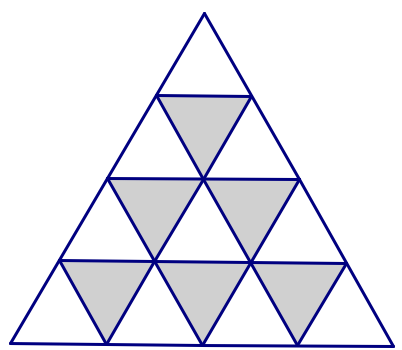
\includegraphics[height=4 cm]{triangleboard}
\end{center}

\end{itemize}

\end{example}

\begin{example}
Recall Problem~\ref{prob:BrokenClock}, ``Squares on a Chess Board'':

\begin{quote}
 This clock has been broken into three pieces.  If you add the numbers in each piece, the sums are consecutive numbers.  Can you break another clock into a different number of pieces so that the sums are consecutive numbers?  
 \begin{center}
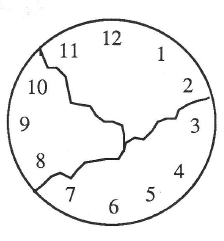
\includegraphics[height=3 cm]{clock}
\end{center}

\end{quote}

The original problem only asks if you can find \emph{one} other way.  The obvious follow-up question: ``Find every possibly way to break the clock into some number of pieces so that the sums of the numbers on each piece are consecutive numbers.  Justify that you have found every possibility.'' 
\end{example}


\begin{thinkpair*}
Choose a problem from the Problem Bank in Section~\ref{sec:ProblemBank} (preferably a problem you have worked on, but that's not strictly necessary).  What follow-up or similar questions could you ask?

\end{thinkpair*}



  

\documentclass[10pt, reqno]{amsart}
% \pdfoutput=1



% Packages to open
\usepackage{amsthm, amssymb, amsmath, enumerate, textcomp}
% \usepackage{fullpage}
\usepackage{verbatim}
\usepackage{graphicx, graphics}
\usepackage{algorithm}
\usepackage{longtable}


% Setup TikZ

\usepackage{tikz}
\usetikzlibrary{arrows}
\tikzstyle{block}=[draw opacity=0.7,line width=1.4cm]

% Hopefully dot packages
\usepackage[all,arc,curve,frame,color]{xy}
\usepackage{subfigure}
\usepackage{url}








% \usepackage{setspace}  % Use command \doublespacing or \onehalfspacing

% Standard Theorem Styles
\newtheorem{thm}{Theorem}[section]
\newtheorem{lem}[thm]{Lemma}
\newtheorem{cor}[thm]{Corollary}
\newtheorem*{cor*}{Corollary}
\newtheorem{prop}[thm]{Proposition}
\newtheorem{obs}[thm]{Observation}
\newtheorem{claim}[thm]{Claim}
\newtheorem*{conjecture*}{Conjecture}
\newtheorem{conjecture}[thm]{Conjecture}
\newtheorem*{thm*}{Theorem}
\newtheorem{ps}{Problem Solving Strategy}

\theoremstyle{remark}
\newtheorem*{question*}{Question}
\newtheorem{question}[thm]{Question}
\newtheorem{answer}[thm]{Answer}
\newtheorem*{remark*}{Remark}
\newtheorem{example}[thm]{Example}
\newtheorem*{thinkpair*}{Think/Pair/Share}



\theoremstyle{definition}
\newtheorem{define}[thm]{Definition}
\newtheorem*{define*}{Definition}
\newtheorem{idea}{Idea}
\newtheorem{problem}{Problem}
\newtheorem{exercise}[thm]{Exercise}
\newtheorem*{problem*}{Problem}
\newtheorem*{sol*}{Solution}


\numberwithin{equation}{section}  % number equations by section

% Standard shortcuts
\newcommand{\LL}{\mathcal{L}}     % Fancy script L
\newcommand{\MM}{\mathcal{M}}  % Fancy script M
\newcommand{\OO}{\mathcal{O}}    % Fancy script O
\newcommand{\FF}{\mathbb{F}}      % Finite field
\newcommand{\ZZ}{\mathbb{Z}}     % Integers
\newcommand{\RR}{\mathbb{R}}     % Reals
\newcommand{\PP}{\mathbb{P}}      % Projective space
\newcommand{\Aff}{\mathbb{A}}      % Affine space
\newcommand{\XX}{\mathcal{X}}      % Model of a variety - script X
\newcommand{\QQ}{\mathbb{Q}}      %Rationals
\newcommand{\CC}{\mathbb{C}}      % Complex Numbers
\newcommand{\mm}{\mathfrak{m}}   % maximal ideal
\newcommand{\pp}{\mathfrak{p}}   % prime ideal
\newcommand{\qq}{\mathfrak{q}}  % another prime ideal
\newcommand{\Gm}{\mathbb{G}_m}  % blackboard bold G for the multiplicative group
\newcommand{\hh}{\mathfrak{h}}  % Upper half plane
\newcommand{\tab}{\hspace{.4cm}} % Tab 



 % Color comments!
\usepackage{xcolor}
% Color comments



%Notes to ourselves
\newcommand{\fellow}[1]{{\color{magenta} \sf $\clubsuit\clubsuit\clubsuit$ Fellow: [#1]}}
\newcommand{\michelle}[1]{{\color{blue} \sf $\clubsuit\clubsuit\clubsuit$ Michelle: [#1]}}


% Some regularly used operator shortcuts
\newcommand{\Hom}{\operatorname{Hom}}
\newcommand{\im}{\operatorname{im}} % Image
\newcommand{\coker}{\operatorname{coker}}  % Cokernel
\newcommand{\Sym}{\operatorname{Sym}}      % Symmetric product
\newcommand{\Spec}{\operatorname{Spec}}
\newcommand{\ord}{\operatorname{ord}}
\newcommand{\Div}{\operatorname{div}}    % Divisor of a rational function
\newcommand{\Gal}{\operatorname{Gal}}  % Galois group
\newcommand{\Gauss}{\operatorname{Gauss}}  % Used for the Gauss point
\newcommand{\supp}{\operatorname{supp}}   % Support
\newcommand{\Pic}{\operatorname{Pic}}        % Picard Groups
\newcommand{\Jac}{\operatorname{Jac}}       % Jacobian Variety
\newcommand{\mult}{\operatorname{mult}}  % multiplicity
\newcommand{\pr}{\operatorname{pr}}     % projection
\newcommand{\sep}[1]{{#1}^{\operatorname{s}}}    % separable closure
\newcommand{\Spf}{\operatorname{Spf}}    % formal spectrum
\newcommand{\Frac}{\operatorname{Frac}}    % Fraction field
\newcommand{\chern}[1]{c_1\left(#1\right)}   % First Chern class
\newcommand{\codim}{\operatorname{codim}}  % codimension
\newcommand{\dist}{\operatorname{dist}}   % distance
\newcommand{\an}[1]{\operatorname{an}}  % analytic space notation
\newcommand{\Aut}{\operatorname{Aut}}   % Automorphism group
\newcommand{\Rat}{\operatorname{Rat}}    % space of rational maps
\newcommand{\PGL}{\operatorname{PGL}}
\newcommand{\PSL}{\operatorname{PSL}}
\newcommand{\alg}[1]{{\overline{#1}}}
\newcommand{\GG}{\mathbb{G}}


% Miscellaneous notational shortcuts
\newcommand{\leftexp}[2]{{\vphantom{#2}}^{#1}{#2}}   % Superscript on the left
\newcommand{\simarrow}{\stackrel{\sim}{\rightarrow}}    % Isomorphic mapping
\newcommand{\ip}[2]{\left\langle #1,#2 \right\rangle} %inner product
\newcommand{\into}{\hookrightarrow}     % Inclusion arrow
\newcommand{\dint}{\int \!\!\! \int}   % double integral
\newcommand{\tth}{^{\operatorname{th}}}
\newcommand{\Berk}{\mathbf{P}}  % Berkovich Projective Space

\newcommand{\Manoa}{M\=anoa}
\newcommand{\Hawaii}{Hawai\kern.05em`\kern.05em\relax i}


% Document Specific Declarations
\newcommand{\id}{\mathrm{id}}
\newcommand{\oo}{\mathfrak{o}}
\DeclareMathOperator{\Per}{Per}
\DeclareMathOperator{\PrePer}{PrePer}
\DeclareMathOperator{\Twist}{Twist}
\DeclareMathOperator{\Ker}{Ker}


%%%%%%%%%%%%%%

\title{Chapter 2: Place Value}





%%%%%%%%%%%%%%


\begin{document}


\maketitle

\fellow{Formatting: can we put things marked ``Problem'' in a box (maybe with some color?) to set it apart?  Same with the Think/Pair/Share (different color?) and Solutions.}

\section{Dots and Boxes}

Here are some dots; in fact there's nine of them.

\begin{center}

\includegraphics[height=3cm]{dots1}
\end{center}

Here are some boxes:

\begin{center}
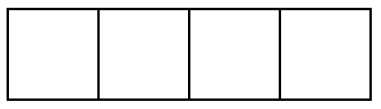
\includegraphics[height=1.5cm]{boxes1}
\end{center}

We're going to a play a game in which boxes explode dots and move them around.  Here's our first rule:

\fellow{Have the rules set off in a box somehow?}

\begin{quote}
{\bf The $1 \leftarrow 2$ Rule:\\
Whenever there are two dots in single box, they ``explode,'' disappear, and become one dot in the box to the left.}
\end{quote}

\begin{example}[Nine dots in the $1 \leftarrow 2$ system]
We start by placing nine dots in the rightmost box.

\begin{center}
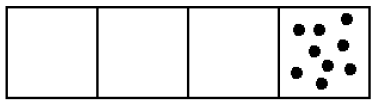
\includegraphics[height=1.5cm]{9dots1}
\end{center}
Two dots in that box explode and become one dot in the box to the left.
\begin{center}
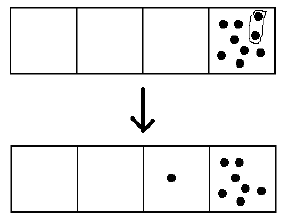
\includegraphics[height=4.5cm]{9dots2}
\end{center}
Since there are more than two dots in the rightmost box, it can happen again.
\begin{center}
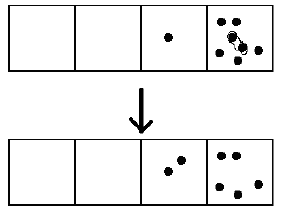
\includegraphics[height=4.5cm]{9dots3}
\end{center}
And again!
\begin{center}
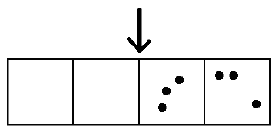
\includegraphics[height=3cm]{9dots4}
\end{center}
Hey, now we have more than two dots in the second box, so those can explode and move!
\begin{center}
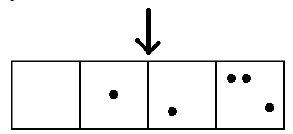
\includegraphics[height=3cm]{9dots5}
\end{center}
And the rightmost box still has more than two dots.
\begin{center}
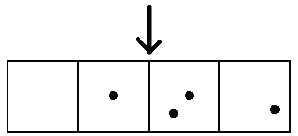
\includegraphics[height=3cm]{9dots6}
\end{center}
Keep going, until no box has two dots.
\begin{center}
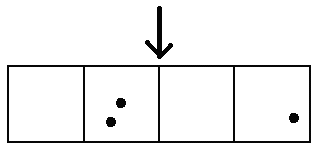
\includegraphics[height=3cm]{9dots7}

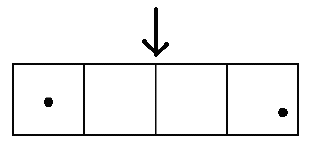
\includegraphics[height=3cm]{9dots8}
\end{center}
After all this, reading from left to right we are left with one dot, followed by zero
dots, zero dots, and one final dot. 

\begin{center}
The $1 \leftarrow 2$ code for nine dots is: \qquad 1001
\end{center}
\end{example}


\subsection*{On Your Own}
Here's a diagram showing what happens for seven dots in a $1 \leftarrow 2$ box.  Trace through the diagram, and circle the pairs of dots that ``exploded'' at each step.

\begin{center}
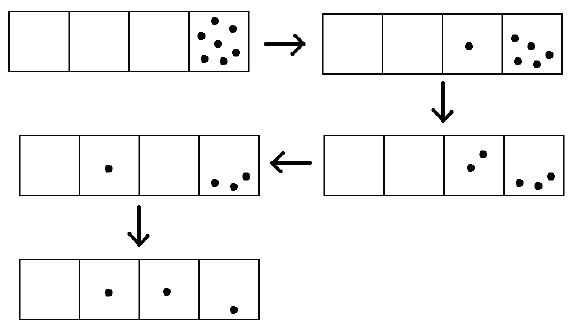
\includegraphics[height=7cm]{7dots}
\end{center}

\begin{center}
The $1 \leftarrow 2$ code for seven dots is: \qquad 111
\end{center}



\begin{problem}
Note: In solving this problem, you don't need to draw on paper; that can get tedious!  Maybe you could use buttons or pennies for dots and do this by hand. What could you use for the boxes?

\begin{enumerate}[(a)]

\item
Draw 10 dots in the right-most box and perform the explosions. What
is the $1 \leftarrow 2$ code for  ten dots?
\item
Find the $1 \leftarrow 2$ code for thirteen dots.
\item
Find the $1 \leftarrow 2$ code for six dots.
\item
What number of dots has $1 \leftarrow 2$ code 101?
\end{enumerate}
\end{problem}

\begin{thinkpair*}
After you worked on the problem, compare your answer with a partner.  Did you both get the same code?  Did you have the same process?
\end{thinkpair*}



\section{Other Rules}
Let's play the dots and boxes game, but change the rule.

\fellow{Have the rules set off in a box somehow?}

\begin{quote}
{\bf The $1 \leftarrow 3$ Rule:\\
Whenever there are three dots in single box, they ``explode,'' disappear, and become one dot in the box to the left.}
\end{quote}

\begin{example}[Fifteen dots in the $1 \leftarrow 3$ system]
Here's what happens with fifteen dots:
\begin{center}
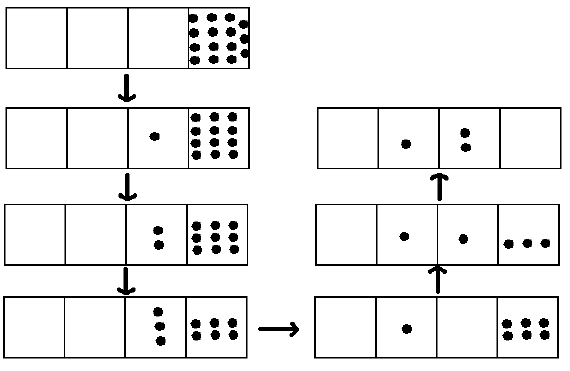
\includegraphics[height=8cm]{15dots}
\end{center}

\begin{center}
The $1 \leftarrow 3$ code for seven dots is: \qquad 120
\end{center}


\end{example}

\begin{problem}\ 

\begin{enumerate}[(a)]
\item
Show that the $1 \leftarrow 3$ code for twenty dots is 202.
\item
Show that the $1 \leftarrow 3$ code for four dots is 11.
\item
What is the  $1 \leftarrow 3$ code for thirteen dots?
\item
What is the  $1 \leftarrow 3$ code for twenty-five dots?
\item
What number of dots has  $1 \leftarrow 3$ code 1022? 
\item
Is it possible for a collection of dots to have  $1 \leftarrow 3$ code 2031?  Explain your answer.

\end{enumerate}
\end{problem}


\begin{problem}\ 

\begin{enumerate}[(a)]
\item
Describe how the $1 \leftarrow 4$ rule would work.
\item
What is the $1 \leftarrow 4$ code for the number thirteen?
\end{enumerate}
\end{problem}

\begin{problem}\ 

\begin{enumerate}[(a)]
\item
What is the $1 \leftarrow 5$ code for the number thirteen?
\item
What is the $1 \leftarrow 5$ code for the number five?
\end{enumerate}
\end{problem}


\begin{problem}\ 

\begin{enumerate}[(a)]
\item
What is the $1 \leftarrow 9$ code for the number thirteen?
\item
What is the $1 \leftarrow 9$ code for the number thirty?
\end{enumerate}
\end{problem}


\begin{problem}\label{prob:Base10}\ 

\begin{enumerate}[(a)]
\item
What is the $1 \leftarrow 10$ code for the number thirteen?
\item
What is the $1 \leftarrow 10$ code for the number thirty-seven?
\item
What is the $1 \leftarrow 10$ code for the number two hundred thirty-eight?
\item
What is the $1 \leftarrow 10$ code for the number five thousand eight hundred and thirty-three?
\end{enumerate}
\end{problem}

\begin{thinkpair*}
After you have worked on the problems on your own, compare your ideas with a partner.  Can you describe what's going on in Problem~\ref{prob:Base10} and why?
\end{thinkpair*}



\section{Binary Numbers}\label{sec:Binary}
Let's go back to the $1 \leftarrow 2$ rule for a moment:
\begin{quote}
{\bf The $1 \leftarrow 2$ Rule:\\
Whenever there are two dots in single box, they ``explode,'' disappear, and become one dot in the box to the left.}
\end{quote}

Two dots in the right-most box is worth one dot in the next box to the left.
\begin{center}
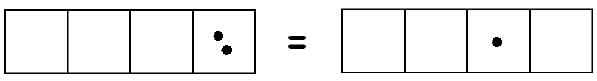
\includegraphics[height=1.5cm]{binary1}
\end{center}
If each of the original dots is worth ``one,'' then the single dot on the left must be worth two.
\begin{center}
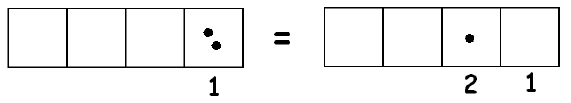
\includegraphics[height=2cm]{binary2}
\end{center}
But we also have two dots in the box of value 2 is worth 1 dot in the box just to the left\dots
\begin{center}
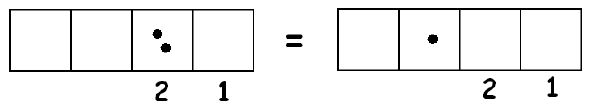
\includegraphics[height=2cm]{binary3}
\end{center}
So that next box must be worth two 2s, which is four!
\begin{center}
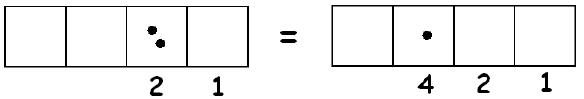
\includegraphics[height=2cm]{binary4}
\end{center}
And two of these fours make eight.
\begin{center}
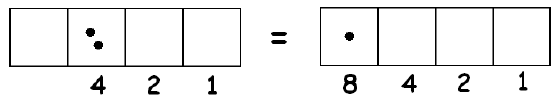
\includegraphics[height=2.1cm]{binary5}
\end{center}


\begin{example}
We said earlier that the $1 \leftarrow 2$ code for nine dots was 1001. Let�s check:
\begin{center}
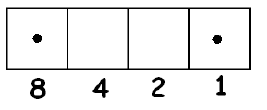
\includegraphics[height=2.1cm]{9inbinary}
\end{center}
\[
8 + 1 = 9,  \text{ so this works!}
\]
We also said that thirteen has $1 \leftarrow 2$ code 1101. This is correct.
\begin{center}
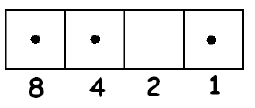
\includegraphics[height=2.1cm]{13inbinary}
\end{center}
\[
\text{Yep!} \quad 8+4+1 = 13.
\]

\end{example}


\begin{problem}\label{prob:BinaryStart}\ 

\begin{enumerate}[(a)]
\item
If there were a box to the left of the 8 box, what would the value of that box be?
\item
What would be the value of a box \emph{two} spots to the left of the 8 box?  Three spots to the left?
\item
What number has $1 \leftarrow 2$ code 100101?
\item
What is the $1 \leftarrow 2$ code for the number two hundred? 
\end{enumerate}
\end{problem}



\begin{define}
Numbers written in the $1 \leftarrow 2$ code are called \emph{binary numbers} or \emph{base two} numbers.  (The prefix ``bi'' means ``two.'')  From now on, when we want to indicate that a number is written in base two, we will write a subscript ``two'' on the number.  So $1001_{\text{two}}$ means ``the number of dots that has $1\leftarrow 2$ code 1001,'' which we already saw was nine.

\end{define}


Important! When we read $1001_{\text{two}}$ we say ``one zero zero one base two.''  We don't say ``one thousand and one,'' because ``thousand'' is not a binary number.



\begin{thinkpair*}
Compare you work on problem~\ref{prob:BinaryStart} with a partner.  
\begin{itemize}
\item
Your first goal: come up with a \emph{general method} to find the number of dots represented by any binary number.  Clearly describe your method.  Test your method out on these numbers, and check your work by actually ``unexploding'' the dots.
\[
1_{\text{two}}
\qquad
101_{\text{two}}
\qquad
1011_{\text{two}}
\qquad
1111_{\text{two}}
\qquad
1101101_{\text{two}}
\]

\item
Explain why binary numbers only contain the digits 0 and 1.

\item
Here is a new (harder) goal: come up with a \emph{general method} to find the binary number related to any number of dots \emph{without actually going through the ``exploding dot'' process}.  Clearly describe your method.  Test your method out on these numbers, and find a way to check your work.
\[
 \text{two dots } = ???_{\text{two}}
\qquad\quad
 \text{seventeen dots } = ???_{\text{two}}
\qquad\quad
 \text{sixty-four dots } = ???_{\text{two}}
 \]
 \[
 \text{sixty-three dots } = ???_{\text{two}}
\qquad\qquad
 \text{one thousand dots } = ???_{\text{two}}
\]
\end{itemize}

\end{thinkpair*}

\subsection{Binary Numbers and Computers}
\fellow{Can you write a \emph{short} description of the use of binary numbers in computers?  Just a paragraph or two getting across the main ideas.}





\section{Other Bases}
In the $1 \leftarrow 3$ system, three dots in one box is worth one dot
in the box one spot to the left. This gives a new picture:
\begin{center}
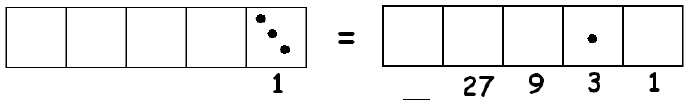
\includegraphics[height=2.1cm]{base3_1}
\end{center}
Each dot in the second box from the left is worth three ones.  Each dot in the third box is worth three 3s, which is nine, and so on.

\begin{example}
We said that the $1\leftarrow 3$ code for fifteen is 120. We see that this is correct
because
\begin{center}
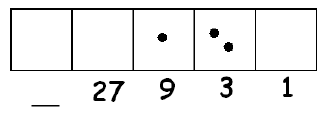
\includegraphics[height=2.5cm]{15base3}
\end{center}
\[
9 + 2\cdot 3 = 9+6 = 15.
\]
\end{example}


\begin{problem}\label{prob:Base3Start}
Answer these questions about the $1 \leftarrow 3$ system.

\begin{enumerate}[(a)]
\item
What label should go on the box to the left of the 27 box?
\item
What would be the value of a box \emph{two} spots to the left of the 27 box?
\item
What number has $1 \leftarrow 3$ code 21002?
\item
What is the $1 \leftarrow 3$ code for the number two hundred?  
\end{enumerate}
\end{problem}

\begin{problem}
In the $1 \leftarrow 4$ system, four dots in one box are worth one dot in the box one place
to the left. 
\begin{enumerate}[(a)]
\item
What is the value of each box?
\begin{center}
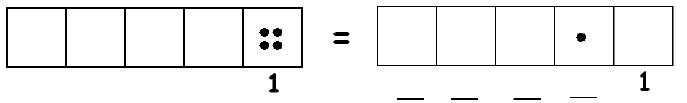
\includegraphics[height=2cm]{base4system}
\end{center}

\item
What is the $1 \leftarrow 4$ code for twenty-nine?

\item
What number has $1 \leftarrow 4$ code 132?
\end{enumerate}

\end{problem}


\begin{problem}
In the $1 \leftarrow 10$ system, ten dots in one box are worth one dot in the box one place
to the left. 
\begin{enumerate}[(a)]
\item
What is the value of each box?
\begin{center}
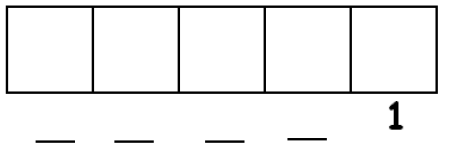
\includegraphics[height=2cm]{base10system}
\end{center}

\item
What is the $1 \leftarrow 10$ code for eight thousand four hundred and twenty-two?

\item
What number has $1 \leftarrow 10$ code 95753?

\item
When we write the number 7842 the ``7'' is represents what quantity? The ``4'' is
four groups of what value? The ``8'' is eight groups of what value? The ``2'' is two
groups of what value?

\item
Why do human beings like the $1\leftarrow 10$ system for writing numbers? 
\end{enumerate}

\end{problem}


\begin{define}
Numbers written in the  $1 \leftarrow 3$ system are called \emph{base three numbers}.  Numbers written in the $1 \leftarrow 4$ system are called \emph{base four numbers}.  Numbers written in the $1 \leftarrow 10$ system are called \emph{base ten numbers}.  In general, numbers written in the $1 \leftarrow b$ system are called \emph{base $b$ numbers.}

\end{define}

In a base $b$ number system, each place represents a \emph{power of $b$}, which means $b^k$ for some positive number $k$.  Remember this means $b$ multiplied by itself $k$ times:
\[
b^k = \underbrace{b \cdot b \cdots b}_{k \text{ times}}.
\]
\begin{itemize}
\item
The right-most place is the \emph{units} or \emph{ones} place.  (Why is this a \emph{power of $b$?})
\item
The second spot is the ``$b$'' place.  (In base 10, it's the tens place.)
\item
The third spot is the ``$b^2$'' place.  (In base 10, that's the hundreds place, and $100 = 10^2$.)
\item
The fourth spot is the ``$b^3$'' place.  (In base 10, that's the thousands place, and $1000 = 10^3$.)
\item
And so on\dots the $n^\text{th}$ spot is the $b^{n-1}$ place.
\end{itemize}

{\bf Notation:}
Whenever we're dealing with numbers written in different bases, we use a subscript to indicate the base so that there can be no confusion.  So $102_\text{three}$ is a base three number,  $222_\text{four}$ is a base four number, and $54321_\text{ten}$ is a base ten number.  If the base is not written, we assume the number is written in base ten. 



\begin{thinkpair*}\ 
\begin{enumerate}[(a)]
\item
Find the number of dots represented by:
\[
102_\text{three}, 
\quad 222_\text{four}, 
\quad 
54321_\text{ten}.
\]
\item
Represent nine dots in each base: 
\begin{center}
 three, four, five, six, seven, eight, nine, and ten.
\end{center}
\item
Which digits are used in the base two system?  The base three system?  The base four system?  The base five system?  The base six system?  The base ten system?
\item
What does the \emph{base} tell you about the number system?  (Think of as many answers as you can!)
\end{enumerate}
\end{thinkpair*}


\subsection{Base $b$ to Base Ten}
In Section \ref{sec:Binary}, you were asked to come up with \emph{general methods} to translate numbers from base two (binary) to  base ten (our standard system).  We're now going to describe some general methods for converting from base $b$  to base ten, where $b$ can represent any whole number bigger than one.

If the base is $b$, that means we're in a $1 \leftarrow b$ system.  A dot in the right-most box is worth 1.  A dot in the second box is worth $b$.  A dot in the third box is worth $b \times b = b^2$, and so on.

\fellow{Can you make a picture of base $b$ boxes with the appropriate labels, say up to  $b^4$?}

So, for example, the number $10123_b$ represents
\[
1\cdot b^4  + 0 \cdot b^3 +  1 \cdot b^2  + 2\cdot b + 3\cdot 1 \text{ dots,}
\]
because we imagine three dots in the right-most box (each worth one), two dots in the second box (each representing $b$ dots), one dot in the third box (representing $b^2$ dots), and so on.  That means we can just do a short calculation to find the total number of dots, without going through all the trouble of drawing the picture and  ``unexploding'' the dots.

\begin{example}
Consider the number $123_\text{five}$.  This represents
\[
 1 \cdot 5^2  + 2 \cdot 5 + 3 = 25 + 10 + 3 = 38 \text{ dots.}
\]
On the other hand,  the number $123_\text{seven}$ represents
\[
 1 \cdot 7^2  + 2 \cdot 7 + 3 = 49 + 14 + 3 = 66 \text{ dots.}
\]

\end{example}


\begin{thinkpair*}\ 
\begin{itemize}
\item
Convert each number to base ten.  Compare your answers with a partner to be sure you agree.

\[
18_\text{nine},
\qquad
547_\text{eight},
\qquad
3033_\text{five},
\qquad
11011_\text{three}.
\]

\item
Which number represents a greater amount of total dots:  
\[
23,455,443_\text{six} \quad \text{ or } \quad 23,455,443_\text{eight}?
\]
  Justify your answer.
\end{itemize}
\end{thinkpair*}


\subsection{Base Ten  to Base $b$}
In Section \ref{sec:Binary}, you were also asked to come up with \emph{general methods} to translate numbers from base ten to  base two.  We're now going to describe some general methods for converting from base ten to  base $b$, where $b$ can represent any whole number bigger than one.

We'll work out an example, and then describe the general method.  

\begin{example}
To convert $321$ to a base five number  (without actually going through the tedious process of exploding $321$ dots in groups of five):


Find the largest power of five that is smaller than 321.  We'll just list powers of five:
\[
5^1 = 5, \quad 5^2 = 25, \quad 5^3 = 125, \quad 5^4 = 625.
\]
So we know that the left-most box we'll use is the $5^3$ box.  
\fellow{add a picture of the appropriately labeled boxes for base 5, up to $5^3$?}

How many dots will be in that left-most box?  That's the same as asking how many 125s are in 321.  Since
\[
2\cdot 125 = 250 \quad \text{ and } \quad 3 \cdot 125 = 375,
\]
we have two dots in the $5^3$ box, representing a total of $250$ dots, but rather than drawing dots we'll start writing the digits to represent them.

\fellow{picture of the base 5 boxes with a ``2'' in  the $5^3$ box?}

How many dots are left unaccounted for?  $321 - 250 = 71$ dots are left.

Now just repeat the process: We can put a ``2'' in the $5^2$ box, and that takes care of $50$ dots.  So so far we have two in the $5^3$ box and two  in the $5^2$ box, so that's a total of 
\[
2\cdot 125 + 2\cdot 25 = 300 \text{ dots}.
\]

\fellow{picture of the base 5 boxes with 2 in $5^3$ box and 2 in the $5^2$ box?}

We have $21$ dots left to account for.  The biggest power of $5$ that's less than 21 is just $5$.  So we can put a ``4'' in the $5$ box, and we have one  left over in the one box.

\fellow{picture of the base 5 boxes with 2 in $5^3$ box and 2 in the $5^2$ box 4 in the $5$ box and 1 in the $1$ box?}

\[
2\cdot 125 + 2\cdot 25 + 4\cdot 5 + 1= 250 + 50 + 20 + 1 =  321 \text{ dots}.
\]
\[
\text{So } 321 = 2241_\text{five}.
\]
\end{example}

The general algorithm to convert from base ten to base $b$:
\begin{enumerate}
\item
Start with your base ten number $n$.  Find the largest \emph{power of $b$} that's less than your number $n$, say that power is $b^k$.  
\item
Figure out how many dots can go in the $b^k$ box without going over the number $n$.  Say that number is $a$.  Put the digit $a$ in the $b^k$ box, and then subtract $n - a\cdot b^k$ to figure out how many dots are left.
\item
If your number is now zero, you accounted for all the dots.  Put zeros in any boxes that remain, and you have the number.  Otherwise, start over at step (1) with the number of dots you have left.

\end{enumerate}

The method seems a little tricky to describe in complete generality.  It's probably better to try a few examples on your own to get the hang of it.

\begin{thinkpair*}
Use the method above to convert $99_\text{ten}$ to base three, to base four, and to base five.
\end{thinkpair*}

The first method we described fills in the boxes from left to right.  Here's another method to convert base ten numbers to another base, and this method fills in the digits from right to left.  Again, we'll start with an example and then describe the general method:

\begin{example}
To convert $712$ to a base seven number:

Divide $712$ by seven and find the quotient and remainder:
\[
712 \div 7 = 101 \text{ R}5.
\]
Put the remainder in the ones place: 
\[
712 = \underline{???}5_\text{seven}.
\]

Now take the quotient and divide by seven to find the quotient and remainder:
\[
101 \div 7 = 14 \text{ R}3.
\]
Put the remainder in the sevens place: 
\[
712 = \underline{???}35_\text{seven}.
\]

Take the previous quotient and divide by seven again:
\[
14 \div 7 = 2 \text{ R}0.
\]
Put the remainder in the $7^2$ place: 
\[
712 = \underline{???}035_\text{seven}.
\]

Since the quotient that's left is less than seven, it goes in the $7^3$ place, and we're done.
\[
712 = 2035_\text{seven}.
\]

Of course, we can (and should!) check our calculation by converting the answer back to base ten:
\[
2035_\text{seven} = 2\cdot 7^3 + 0 \cdot 7^2 + 3 \cdot 7 + 5 
= 686 + 0 + 21 + 5 = 712_\text{ten}.
\]

\end{example}

So here's a second general method for converting base ten numbers to an arbitrary base $b$:
\begin{enumerate}
\item
Divide the base ten number by $b$ to get a quotient and a remainder. 
\item
Put the remainder in the right-most space in the base $b$ number.
\item
If the quotient is less than $b$, it goes in the space one spot to the left.  Otherwise, go back to step (1) and repeat it with the quotient, filling in the remainders from right to left in the base $b$ number.
\end{enumerate}

We can use the dots and boxes system to explain why this method of quotients and remainders works.   It's not just a ``trick!''  We'll stick with the example of converting $712$ to base seven, so we have something specific to talk about.


\begin{itemize}
\item
We imagine 712 dots in the right-most box, since that represents 712 dots total.  Since we're converting to base seven, we're in the $1 \leftarrow 7$ system.
\fellow{picture of the base seven boxes up to $7^3$ with just the number 721 in the right-most box.}


\item
Groups of seven dots will explode, and each group of seven becomes one dot in the next box.  How many groups of seven dots are there?  Well, there are 101 groups of seven, with 5 dots left over out of a group.  That's what we figured out with the calculation
\[
712 \div 7 = 101 \text{ R}5.
\]

\item
Imagine we explode all the groups of seven that we can make in the right-most box before we move on.  Then we would have
 5 dots left in that first  box, and 101 dots in the second box.  
 
 \fellow{picture of the base seven boxes up to $7^3$ with  the number 5 in the rightmost box and 101 in the  in the second box.}

 
 \item
 Again, groups of seven dots will explode, and each group becomes one dot in the third box.  How many groups of seven dots are there?  There are 14 groups with three left over.  That's what we computed like this:
\[
101 \div 7 = 14 \text{ R}3.
\]

 \fellow{picture of the base seven boxes up to $7^3$ with  the number 5 in the rightmost box and 3 in the  in the second box and 14 in the third box.}


\item
OK, now there are 5 dots in the right-most box, 3 dots in the second box, and 14 dots in the third box.  We do it all again!  Groups of seven explode, and each group forms  dot in the next box to the left.  Fourteen dots gives two equal groups of seven, none left over.  

\item
So we end up with: 5 dots in the right-most box, 3 dots in the second box, zero dots in the third box, and 2 dots in the fourth box.  And there's nothing left to explode!

 \fellow{picture of the base seven boxes up to $7^3$ with  the number 5 in the rightmost box and 3 in the  in the second box and 0 in the third box and 2 in the last box.}


\item
Now we can read off the number left-to-right:
\[
712 = 2035_\text{seven}.
\]

\end{itemize}


Again, the method probably makes more sense if you try it out a few times.  

\begin{thinkpair*}
Use the method described above to convert $250_\text{ten}$ to base three, four, five, and six.  For each of the computations, write a careful dots-and-boxes explanation for why it works.
\end{thinkpair*}






\section{Number Systems}

\subsection{History}
\fellow{Can you write a \emph{short} history / description of some different systems like the Egyptian, Mayan, and Roman numerals.  What's in the book is totally overkill and too much.  No need to have students do any problems.  Just a few paragraphs describing additive system versus positional system and giving a couple of examples.}





\subsection{Fibonacci}
\fellow{Include a picture and \emph{short} bio of Fibonacci?  What he really \emph{should} be famous for is giving us the arabic numerals and showing the ease of computation with a positional system, not the sequence of numbers that came from one little problem in his book... Get across where the base 10 system was created, and that Fibonacci brought it to the Western world from which it spread?}



\begin{problem}\label{prob:timesnine}
What is the difference between $5_\text{nine}$ and $50_\text{nine}$?  
\end{problem}


\begin{problem}\label{prob:timesfive}
Convert each base-$5$ number to a base-$10$ number.  Look for a shortcut!

\[
4_{\text{five}}
\qquad
40_{\text{five}}
\qquad
400_{\text{five}}
\qquad
4000_{\text{five}}
\]
\[
\text{\bf Challenges: }\quad
0.4_{\text{five}}
\quad
0.04_{\text{five}}
\]

\end{problem}

\begin{thinkpair*}
Discuss your answers to problems \ref{prob:timesnine} and \ref{prob:timesfive}.  Discuss:
\begin{itemize}
\item
When you add zeros to the right of a number in base ten, what does that do to the number?  (Think about 2, 20, 200, 2000, etc.).
\item
When you add zeros to the right of a number in base nine, what does that do to the number?
\item
When you add zeros to the right of a number in base five, what does that do to the number?
\item
When you add zeros to the right of a number in base $b$, what does that do to the number?
\end{itemize}
\end{thinkpair*}



\section{Even Numbers}
How do we know if a number is even?  What does it mean?
Well, some number of dots is \emph{even} if I can divide the dots into pairs, and every dot has a partner.
\fellow{Add a picture of pairs of dots grouped together?  A fairly large number would be good.}

And some number of dots is \emph{odd} if, when I try to pair up the dots, I always have a single dot left over with no partner.
\fellow{Add a picture of an odd number of dots?}


The number of dots is either even or odd.  It's a property of the \emph{quantity} and is doesn't change when you write the number in different bases.  

\begin{problem}\label{prob:WhichEven}
Which of these numbers represent an even number of dots?  Explain how you decide.
\[
22_\text{ten} \qquad
319_\text{ten} \qquad
133_\text{five} \qquad
222_\text{five} \qquad
11_\text{seven} \qquad
11_\text{four} \qquad
\]
\end{problem}


\begin{thinkpair*}
Compare your answers to problem \ref{prob:WhichEven} with a partner.  Then try these together:

\begin{enumerate}[(a)]
\item
Count  by twos to $20_{\text{ten}}$.


\item
Count  by twos to $30_{\text{four}}$.


\item
Count  by twos  to $51_{\text{seven}}$.
\end{enumerate}


\end{thinkpair*}


\begin{thinkpair*}
You know that you can tell if a number in base 10 is even just by looking at the units digit.  Which one of the following statements \emph{best} captures the reason for this rule?

\begin{enumerate}
\item
It works because even and odd numbers alternate, so you only have to look at the ones place.


\item
It works if the number ends with an even digit, but it only works for whole numbers and decimals (e.g. 12 and $1.2$.).



\item
It actually only works if the last digit is 2, 4, 6, or 8.


\item
It works because all digits other than the units digit --- for example tens, hundreds, and thousands --- represent even numbers, and sums of even numbers are even.
\end{enumerate}

\end{thinkpair*}


\begin{problem}\label{prob:evenbase7}\ 
\begin{enumerate}[(a)]
\item
Write the numbers zero through fifteen in base seven:
\[
0_\text{seven}, 1_\text{seven}, 2_\text{seven}, \ldots
\]
\item
Circle all of the even numbers in your list.  How do you know they are even?
\item
Find a rule: how can you tell if a number is even when it's written in base seven?
\end{enumerate}

\end{problem}


\begin{problem}\label{prob:evenbase4}\ 
\begin{enumerate}[(a)]
\item
Write the numbers zero through fifteen in base four:
\[
0_\text{four}, 1_\text{four}, 2_\text{four}, \ldots
\]
\item
Circle all of the even numbers in your list.  How do you know they are even?
\item
Find a rule: how can you tell if a number is even when it's written in base four?
\end{enumerate}

\end{problem}


\begin{thinkpair*}
Discuss your answers to problems \ref{prob:evenbase7} and \ref{prob:evenbase4}.  
\begin{itemize}
\item
Why are the rules for even numbers different in different bases?  
\item
For either your base four rule or your base seven rule, can you explain \emph{why} it works that way?
\end{itemize}

\end{thinkpair*}




\section{Orders of Magnitude}
\begin{problem}\label{prob:millionsecs}
How old were you when you were one million seconds old?  (That's $1,000,000$.)
\begin{itemize}
\item
Before you figure it out, write down a guess.  What's your gut instinct?  About a day?  A week?  A month?  A year?  Have you already reached that age?  Or maybe you won't live that long?
\item
Now figure it out!  When was / will be your million-second birthday?
\end{itemize}
\end{problem}

\begin{problem}\label{prob:billionsecs}
How old were you when you were one \emph{billion} seconds old?  (That's $1,000,000,000$.)
\begin{itemize}
\item
Again, before you figure it out, write down a guess.  
\item
Now figure it out!  When was / will be your billion-second birthday?
\end{itemize}
\end{problem}

Were you surprised by the answers?  People (most people, anyway) tend to have a very good sense for small, everyday numbers, but have very bad instincts about big numbers.  One problem is that we tend to think \emph{additively}, as if one billion is about a million plus a million more (give or take).  But we need to think \emph{mulitplicatively} in situations like this.  One billion is $1,000 \times$ a million.  

So you could have just taken your answer to problem \ref{prob:millionsecs} and multiplied it by $1,000$ to get your answer to problem \ref{prob:millionsecs}.  Of course, you would probably still need to do some calculations to make sense of the answer.


\begin{thinkpair*}
When is your one trillion second birthday?  What will you do to celebrate?
\end{thinkpair*}



\begin{thinkpair*}
The US debt is total amount the government has borrowed.  (This borrowing covers the \emph{deficit} --- the difference between what the government spends and what it collects in taxes.)  In summer of 2013, the US debt was  \emph{on the order of} 10 trillion dollars.  (That means more than 10 trillion but less than 100 trillion.  If you were to write out the dots-and-boxes picture, the dots would be as far left as the $10,000,000,000$ place.)

\begin{itemize}
\item
If the US pays back one penny every second, will the national debt be paid off in your lifetime?  Explain your answer.
\item
A headline from April 2013 said, ``US to Pay Down \$35 billion in Quarter 2.''  Suppose the US pays down \$35 billion dollars \emph{every} quarter (so four times per year).  About how many  years would it take to pay of the total national debt?
\end{itemize}
\end{thinkpair*}



Here are some big-number problems to think about.  Can you solve them?

\begin{problem}\ 
\begin{enumerate}
\item 
Suppose you have a million jelly beans, and you tile the floor with them.  How big of an area will they cover?  The classroom?  A football field?  Something bigger?  What if it was a billion jelly beans?

\item
Suppose you have a million jelly beans and you stack them up.  How tall would it be?  As tall as you?  As a tree?  As a skyscraper?  What if it was a billion jelly beans?  About how many jelly beans (what \emph{order of magnitude}) would you need to stack up to reach the moon?  Explain your answers.

\end{enumerate}

\end{problem}



\subsection{Fermi Problems}
James Boswell wrote,``Knowledge is of two kinds.  We know a subject ourselves, or we know where we can find information upon it.'' 

But math proves this wrong.  There is actually a third kind of knowledge: Knowledge that you \emph{figure out for yourself}.
In fact, this is what scientists and mathematicians do for a living: they create new knowledge!  Starting with what is already known, they ask ``what if\dots'' questions.  And eventually, they figure out something new, something no one ever knew before!

Ever for knowledge that you \emph{could} look up (or ask someone), you can often figure out the answer (or a close approximation to the answer) on your own.  You need to use a little knowledge, and a little ingenuity.

 Fermi problems, named for the physicist Enrico Fermi, involve using your knowledge, making educated guesses, and doing reasonable calculations to come up with an answer that might at first seem unanswerable.
 

\begin{example}
Here's a classic Fermi problem: How many elementary school teachers are there in the state of Hawaii?

You might think: How could I possibly answer that?  Why not just google it?  (But some Fermi problems we meet will have --- gasp! --- non-googleable answers.)

First let's define our terms.  We'll say that we care about classroom teachers (not administrators, supervisors, or other school personnel) who have a permanent position (not a sub, an aide, a resource room teacher, or a student teacher) in a grade K--5 classroom.

But let's stop and think.  Do you know the population of Hawaii?  It's about $1,000,000$ people.  (That's not exact, of course.  But this is an exercise is estimation.  We're trying to get at the \emph{order of magnitude} of the answer.)

How many of those people are elementary school students?  Well, what do you know about the population of Hawaii?  Or what do you \emph{suspect} is true?  A reasonable guess would be that the population is evenly distributed across all age groups.  Something like this?  We'll assume people don't live past 80.  (Of course some people do!  But we're all about making simplifying assumptions right now.  That gives us 8 age categories, with about 125,000 people in each category.

\begin{center}
\begin{tabular}{ l | l}\\
age range & \# people \\ \hline
 0 -- 9 &125,000 \\
 10 -- 19 &125,000 \\
 20 -- 29 &125,000 \\
 30 -- 39 &125,000 \\
 40 -- 49 &125,000 \\
 50 -- 59 &125,000 \\
 60 -- 69 &125,000 \\
 70 -- 79 & 125,000\\
\end{tabular}
\end{center}


An even better guess (since we have a large university that draws lots of students) is that there's a ``bump'' around college age.  And some people live past 80, but  there are probably fewer people in the older age brackets.  Maybe the breakdown is something like this?  (If you have better guesses, use them!)


\begin{center}

\begin{tabular}{ l | l}\\
age range & \# people \\ \hline
 0 -- 9 &125,000 \\
 10 -- 19 &130,000 \\
 20 -- 29 & 140,000\\
 30 -- 39 & 125,000\\
 40 -- 49 &125,000 \\
 50 -- 59 &125,000 \\
 60 -- 69 & 120,000\\
 $> 70$ & 105,000 \\
\end{tabular}
\end{center}



So, how many K--5 students are in Hawaii?  That covers six years of the 0--9 (maybe 10) range.  If we are still going with about the same number of people at each age, there should be about 12,500 in each grade for a total of $12,500\times 6 = 75,000$ K--5 students.

OK, but we really wanted to know about K--5 \emph{teachers}.  One nice thing about elementary school: there tends to be just one teacher per class.  So we need an estimate of how many classes, and that will tell us how many teachers.

So, how many students in each class?  It probably varies a bit, with smaller kindergarten classes (since they are more rambunctious and need more attention), and larger fifth grade classes.  There are also smaller classes in private schools and charter schools, but larger classes in public schools.  So a reasonable average might be $25$ students per class across all grades K--5 and all schools?

So that makes $75,000 \div 25 = 3,000$ K--5 classrooms in Hawaii.  And that should be the same as the number of K--5 teachers.


\end{example}

\begin{problem}
How good is this estimate?  Can you think of a way to check and find out for sure?
\end{problem}

So now you see the process:
\begin{itemize}
\item
Define your terms.
\item
Write down what you know.
\item
Make some reasonable guesses / estimates.
\item
Do some simple calculations.
\end{itemize}

It's your turn to try your hand at some Fermi problems.

\begin{problem}
How much money does UH Manoa earn in parking revenue each year?
\end{problem}


\begin{problem}
How many tourists visit Waikiki in a year? 
\end{problem}

\begin{problem}
How much gas would be saved in Hawaii if one out of every ten people switched to a carpool? 
\end{problem}



\begin{problem}
How high can a climber go up a mountain on the energy in one chocolate bar? 
\end{problem}



\begin{problem}
How much pizza is consumed by UH Manoa students in a month? 
\end{problem}


\begin{problem}
How much would it cost to provide free day care to every 4th grader in the US? 
\end{problem}

\begin{problem}
How many books are in Hamilton library? 
\end{problem}


\begin{problem}
Make up your own Fermi problem\dots what would you be interested in calculating?  Then try to solve it!
\end{problem}





\section{Problem Bank}


\begin{problem}\ 

\begin{enumerate}[(a)]
\item
If you were counting in base four, what number would you say just before you said $100_{\text{four}}$?

\item
What number is one more than $133_{\text{four}}$?


\item
What is the greatest three-digit number that can be written in base four?  What numbers come just before and just after that number?
\end{enumerate}


\end{problem}


\begin{problem}
Explain what is wrong with writing $313_\text{two}$ or $28_\text{eight}$.
\end{problem}



\begin{problem}\ 
\begin{enumerate}[(a)]
\item
Write out the base three numbers from $1_\text{three}$ to $200_\text{three}$.
\item
Write out the base five numbers from $1_\text{five}$ to $100_\text{five}$.
\item
Write the  four base six numbers that come after $154_\text{six}$.
\end{enumerate}

\end{problem}

\begin{problem}
Convert each base-$4$ number to a base-$10$ number.  Explain how you did it.

\[
 13_{\text{four}}
\qquad
322_{\text{four}}
\qquad
101_{\text{four}}
\qquad
1300_{\text{four}}
\]
\[
\text{\bf Challenges: }\quad
0.2_{\text{four}}
\qquad
0.111..._{\text{four}}=0.\overline{1}_{\text{four}}
\]
\end{problem}



\begin{problem}
Convert each base-$10$ number to a base-$4$ number.  Explain how you did it.

\[
13
\qquad
8
\qquad
24
\qquad
49
\]
\[
\text{\bf Challenges: }\quad
0.125
\qquad
0.111...=0.\overline{1}
\]


\end{problem}






\begin{problem}
In order to use base sixteen, we need sixteen digits --- they will represent the numbers zero through fifteen.  We can use our usual digits 0 -- 9, but we need \emph{new symbols} to represent the \emph{digits} ten, eleven, twelve, thirteen, fourteen, and fifteen.  Here's one standard convention:

\begin{center}
\begin{tabular}{| c | c |}\hline
{\bf base 10 number} & {\bf base 16 digit} \\ \hline\hline
10 & A\\ \hline
11 & B \\ \hline
12 & C \\ \hline
13 & D \\ \hline
14 & E \\ \hline
15 & F \\ \hline
\end{tabular}
\end{center}

\begin{enumerate}[(a)]
\item
Convert these numbers from base sixteen to base ten, and show your work:
\[
6\textup{D}_{\text{sixteen}} 
\qquad \quad
\textup{AE}_{\text{sixteen}} 
\qquad\quad
9\textup{C}_{\text{sixteen}} 
\qquad\quad
2\textup{B}_{\text{sixteen}} 
\]



\item
Convert these numbers from base ten to base sixteen, and show your work:
\[
97 
\qquad \quad
144
\qquad\quad
203
\qquad\quad
890
\]
\end{enumerate}

\end{problem}


\begin{problem}
How many different symbols would you need for a base twenty-five system?  Justify your answer.
\end{problem}


\begin{problem}
All of the following numbers are multiples of three. 
\[
3, \quad 6, \quad 9, \quad 12, \quad 21,  \quad 27, \quad 33, \quad 60, \quad 81, \quad 99.
\]
\begin{enumerate}[(a)]
\item
Identify the \emph{powers of $3$} in the list.  Justify your answer.
\item
Write each of the numbers above in base three.
\item
In base three: how can you recognize a \emph{multiple of $3$}?  Explain your answer.
\item
In base three: how can you recognize a \emph{power of $3$}?  Explain your answer.
\end{enumerate}
\end{problem}


\begin{problem}
All of the following numbers are multiples of five. 
\[
5, \quad 10, \quad 15, \quad 25, \quad 55,  \quad 75, \quad 100, \quad 125, \quad 625, \quad 1000.
\]
\begin{enumerate}[(a)]
\item
Identify the \emph{powers of $5$} in the list.  Justify your answer.
\item
Write each of the numbers above in base five.
\item
In base five: how can you recognize a \emph{multiple of $5$}?  Explain your answer.
\item
In base five: how can you recognize a \emph{power of $5$}?  Explain your answer.
\end{enumerate}
\end{problem}




\begin{problem}
Convert each number to the given base.
\begin{enumerate}[(a)]
\item
$395_\text{ten}$ into base eight.
\item
$52_\text{ten}$ into base two.
\item
$743_\text{ten}$ into base five.

\end{enumerate}
\end{problem}



\begin{problem}
What bases makes theses equations true?  Justify your answers.

\begin{enumerate}[(a)]
\item
$ 35 = 120_{\text{\underline{\quad}}}  $


\item
$ 41_{\text{six}} = 27_{\text{\underline{\quad}}}  $


\item
$ 52_{\text{seven}} = 34_{\text{\underline{\quad}}}  $



\end{enumerate}

\end{problem}



\begin{problem}
What bases makes theses equations true?

\begin{enumerate}[(a)]
\item
$ 32 = 44_{\text{\underline{\quad}}}  $


\item
$ 57_{\text{eight}} = 10_{\text{\underline{\quad}}}  $


\item
$ 31_{\text{four}} = 11_{\text{\underline{\quad}}}  $


\item
$ 15_x = 30_y  $



\end{enumerate}



\end{problem}









\begin{problem}\ 
\begin{enumerate}[(a)]
\item
Find a base ten number that is twice the product of its two digits.  
Is there more than one answer?  Justify what you say.

\item
Can you solve this problem in any base other than ten?
\end{enumerate}
\end{problem}



\begin{problem}\ 
\begin{enumerate}[(a)]
\item
I have a four-digit number written in base ten.
When I multiply my number by four, the digits get reversed.

\item
Can you solve this problem in any base other than ten?
\end{enumerate}
\end{problem}



\begin{problem}
Consider this base ten number
(I got this by writing the numbers from 1 to 60 in order next to one another):


\[
12345678910111213\ldots57585960
\]




\begin{enumerate}[(a)]
\item
 What is the largest number that can be produced by erasing one hundred digits of the number?  (When you erase a digit it goes away.  For example, if you start with the number $12345$ and erase the middle digit, you produce the number $1245$.)  How do you \emph{know} you got the largest possible number?


\item
 What is the smallest number that can be produced by erasing one hundred digits of the number?  How do you \emph{know} you got the smallest possible number?


\end{enumerate}



\end{problem}




\begin{problem}
Can you find numbers (not necessarily single digits!) $a$ and $b$ so that $a_b = b_a$?  
Can you find more than one solution?  What must be true of $a$ and $b$?  Justify your answers.

\end{problem}





\section{Exploration}

\begin{problem}
Jay decides to play with a system that follows a $1 \leftarrow 1$ rule. He
puts one dot into the right-most box. What happens?
\begin{center}
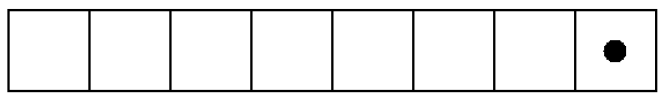
\includegraphics[height=1.5cm]{adventure1}
\end{center}

\end{problem}


\begin{problem}\label{prob:base1.5}
Poindexter decides to play with a system that follows
the rule $2\leftarrow 3$.
\begin{enumerate}[(a)]
\item
Describe what this rule does when there are three dots in the right-most box.
\item
Draw diagrams or use buttons or pennies to find the $2\leftarrow 3$ codes for the
following numbers:
\[
1, 2, 3, 4, 5, 6, 7, 8, 9, 10, 11, 12, 13, 14, 15, 16, 17, 18, 19, 20, 24, 27, 30, 33, 36, \text{ and }
39
\]
Can you find (and \emph{explain}) any patterns?
\end{enumerate}
\end{problem}


\begin{problem}
Repeat problem \ref{prob:base1.5} for your own rule. Choose two numbers $a$ and $b$ and figure
out what the code is for your $a\leftarrow b$ system for each of the numbers above.
\end{problem}

\end{document}


  



\chapter{Numbers \& Operations}






\fellow{Formatting: can we put things marked ``Problem'' in a box (maybe with some color?) to set it apart?  Same with the Think/Pair/Share (different color?) and Solutions.}


When learning and teaching about arithmetic, it helps to have mental and physical \emph{models} for what the operations mean.  That way, when you are presented with an unfamiliar problem or a question about why something is true, you can often work it out using the model --- this might mean  dawning pictures, using physical materials (manipulatives), or just thinking about the model to help you reason out the answer.

\begin{thinkpair*}
Write down your mental models for each of the four basic operations.  What do they actually \emph{mean}?  How would you explain them to a second grader?  What pictures could you draw for each operation? Think about each one separately, as well as how they relate to each other:
\begin{itemize}
\item
addition
\item
subtraction
\item
multiplication, and
\item
division.
\end{itemize}

After writing down your own ideas, share them with a partner.  Do you and your partner have the same models for each of the operations or do you think about them differently?
\end{thinkpair*}

Teachers should have lots of mental models --- lots of ways to explain the same concept.  In this chapter, we'll look at some different ways to understand the four basic arithmetic operations. 
First, let's define some terms:
\begin{define}
\emph{Counting numbers} are literally the numbers we use for counting: $1, 2, 3, 4, 5, \dots$.  These are sometimes called the \emph{natural numbers} by mathematicians, and they are represented by the symbol $\mathbb N$.

\emph{Whole numbers} are the counting numbers together with $0$.

\emph{Integers} include the positive and negative whole numbers, and mathematicians represent these with the symbol $\mathbb Z$.  (This comes from German, where the word for ``number'' is ``z\"ahlen.'')
\end{define}



\section{Model 1: Dots and Boxes}

We already have a natural model for thinking about counting numbers: a number is a quantity of dots.  Depending on which number system you use, you might write down the number in different ways.  But the  quantity of dots is a counting number, however you write it down.

\subsection{Addition as combining}
For now, we'll focus on the base-10 system.  Here's how we think about the number 273 in that system:
\begin{center}
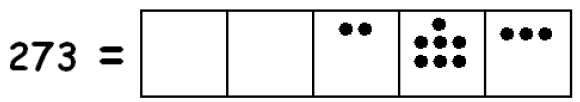
\includegraphics[height=2cm]{273base10}
\end{center}
And here is the number 512:
\begin{center}
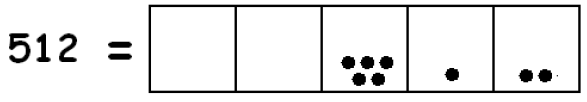
\includegraphics[height=2cm]{512base10}
\end{center}


\fellow{Most of these addition / subtraction examples might be nicer as animations, if we can do that!}

\begin{example}[$273+512$]
We can add these in the natural way: just combine the piles of dots.  Since they're already in place-value columns, we can combine dots from the two numbers that are in the same place-value box.
\begin{center}
\qquad\qquad\qquad\qquad
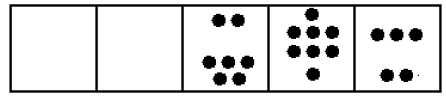
\includegraphics[height=2cm]{785base10}
\end{center}
We can count up the answer: there are 7 dots in the hundreds box, 8 dots in the tens box, and 5 dots in the ones box.

\begin{center}
\begin{tabular}{rl}
& 273\\
+ & 512\\ \hline
& 785
\end{tabular}
\end{center}

And saying out the long way we have:
\begin{itemize}
\item
Two hundreds plus five hundreds gives 7 hundreds.
\item
Seven tens plus one ten gives 8 tens.
\item
Three ones plus 2 ones gives 5 ones.
\end{itemize}
This is the answer 785.
\end{example}

\begin{example}[$163+489$]
Let's do another one.  Consider $163+489$.
\begin{center}
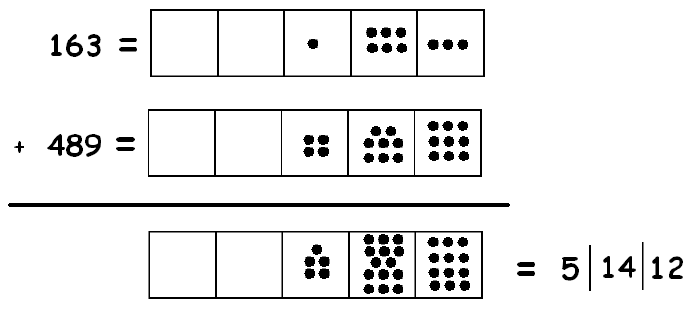
\includegraphics[height=5cm]{base10add1}

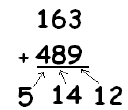
\includegraphics[height=2cm]{base10add2}
\end{center}

And this is absolutely mathematically correct:
\begin{itemize}
\item
One hundred plus four hundreds does give 5 hundreds.
\item
Six tens plus eight tens does give 14 tens.
\item
Three ones plus nine ones does give 12 ones.
\end{itemize}
The answer is $5 \mid 14 \mid 12$, which we might try to pronounce as``five hundred and
fourteeny-tenty twelvety!'' (Oh my!)

The trouble with this answer  is that most of the rest of the
world wouldn't understand what we are talking about! Since this is a base 10 system,
we can do some explosions.

\begin{center}
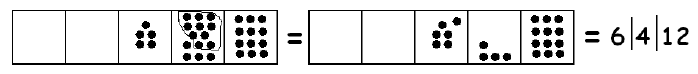
\includegraphics[height=1.4cm]{base10add3}
\end{center}
The answer now looks like ``six hundred forty twelvety''! Still not a familiar number, so let's do another
explosion:

\begin{center}
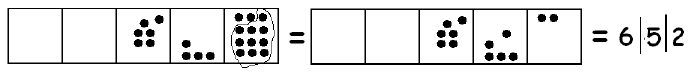
\includegraphics[height=1.5cm]{base10add4}
\end{center}
The answer is ``six hundred fifty two.'' Okay, the world can understand this one!
\begin{center}
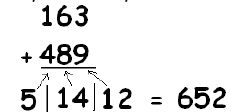
\includegraphics[height=2cm]{base10add5}
\end{center}
\end{example}


\begin{thinkpair*}
Solve the following exercises by thinking about the dots and boxes.
(You can draw the pictures, or just imagine them.) Then translate the answer into
something the rest of the world can understand.
\begin{center}
\begin{tabular}{rl}
& 148\\
+ & 323\\ \hline
\\
\end{tabular}
\qquad
\begin{tabular}{rl}
& 567\\
+ & 271\\ \hline
\\
\end{tabular}
\qquad
\begin{tabular}{rl}
& 377\\
+ & 188\\ \hline
\\
\end{tabular}
\qquad
\begin{tabular}{rl}
& 582\\
+ & 714\\ \hline
\\
\end{tabular}

\begin{tabular}{rl}
& 310462872\\
+ & 389107123\\ \hline
\\
\end{tabular}
\qquad
\begin{tabular}{cccccccccc}
& 872637163\\
+ & 187782748\\ \hline
\\
\end{tabular}

\end{center}
\end{thinkpair*}


\begin{problem}
Use the dots and boxes technique to solve these problems.  \emph{Do not convert to base 10!  Try to work directly in the base given.}  It might help to actually draw the pictures.

\begin{center}
\begin{tabular}{rl}
& $20413_\text{five}$ \\
+ & $13244_\text{five}$\\ \hline
\\
\end{tabular}
\qquad
\begin{tabular}{rl}
& $4052_\text{nine}$ \\
+ & $6288_\text{nine}$ \\ \hline
\\
\end{tabular}
\qquad
\begin{tabular}{rl}
& $3323_\text{seven}$ \\
+ & $3555_\text{seven}$ \\ \hline
\\
\end{tabular}
\end{center}

\end{problem}





\subsection{The Standard Algorithm for Addition}
Let's go back to the example $163 + 489$. Some teachers don't like writing:
\begin{center}
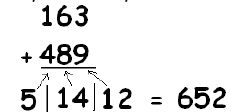
\includegraphics[height=2cm]{base10add5}
\end{center}

They prefer to teach their students to start with the 3 and 9 at the end and sum
those to get 12. This is of course correct --- we got 12 as well.
\begin{center}
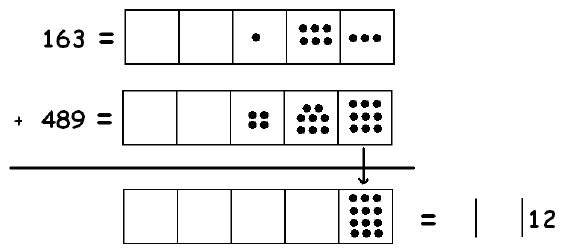
\includegraphics[height=5cm]{base10add6}
\end{center}
But they don't want students to write or think ``twelvety,''  so they have their students write something like this:
\begin{center}
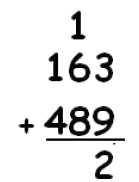
\includegraphics[height=2cm]{base10add8}
\end{center}
which can seem completely mysterious.
What's really going on?  They are exploding ten dots, of course!
\begin{center}
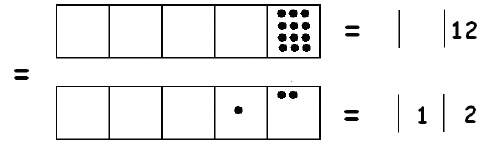
\includegraphics[height=3cm]{base10add7}
\end{center}

Now we carry on with the problem and add the tens.  Students are taught to write:
\begin{center}
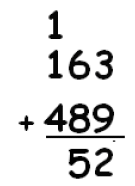
\includegraphics[height=2cm]{base10add10}
\end{center}
But what this means is better shown in this picture:
\begin{center}
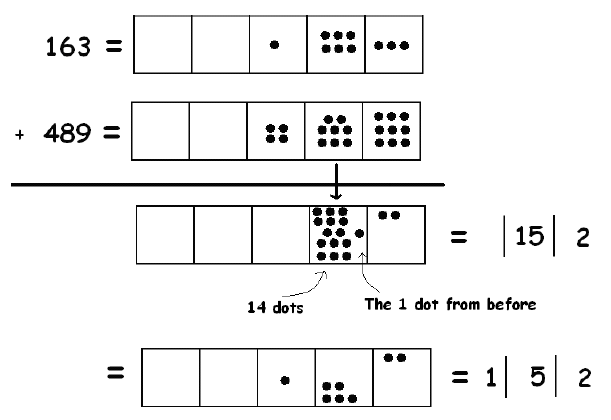
\includegraphics[height=7.5cm]{base10add9}
\end{center}

And now we finish the problem.
\begin{center}
\includegraphics[height=5cm]{base10add11}

\bigskip
\includegraphics[height=2cm]{base10add12}

\end{center}


In the standard algorithm, we work from right to left, doing the ``explosions'' as we go along. This means
that we start adding at the ones place  and work towards the left-most place value,
``carrying'' digits that come from the explosions.  (This is really not carrying; a better for it is \emph{regrouping}.  Ten ones become one ten.  Ten tens become one hundred.  And so on.)

In the dots and boxes method, we add in any direction or order we like and then we do
the explosions at the end.
\begin{itemize}
\item
{\bf Why do we like the standard algorithm?}  Because it is efficient.
\item
{\bf Why do we like the dots and goes method?} Because it is easy to
understand.
\end{itemize}

\begin{thinkpair*}
Redo the problems below using the standard algorithm. You will see that
it is quicker.
\begin{center}
\begin{tabular}{rl}
& 148\\
+ & 323\\ \hline
\\
\end{tabular}
\qquad
\begin{tabular}{rl}
& 567\\
+ & 271\\ \hline
\\
\end{tabular}
\qquad
\begin{tabular}{rl}
& 377\\
+ & 188\\ \hline
\\
\end{tabular}
\qquad
\begin{tabular}{rl}
& 582\\
+ & 714\\ \hline
\\
\end{tabular}

\begin{tabular}{rl}
& 310462872\\
+ & 389107123\\ \hline
\\
\end{tabular}
\qquad
\begin{tabular}{cccccccccc}
& 872637163\\
+ & 187782748\\ \hline
\\
\end{tabular}
\end{center}

\end{thinkpair*}


\subsection{Subtraction as take-away}  In addition, we started with two collections of dots (two numbers), and we \emph{combined} them to form one bigger collection.  That's pretty much the definition of addition: combining two collections of objects.
  In subtraction, we start with one collection of dots (one number), and we take some dots away.


\begin{example}[$376-125$]
Suppose we want to find $376 - 125$ in the dots and boxes model.  We start with the representation of $376$:

\fellow{add picture of dots \& boxes for 376?}

Since we want to ``take away'' 125, that means we take away  one dot from the hundreds box, leaving two dots.  We take away two dots from the tens box, leaving five dots.  And we take away five dots from the ones box, leaving one dot.

\fellow{add picture of dots \& boxes for 251? Would be cool if we can see shadows or erasure of the 125.  If not, maybe an intermediate picture where the appropriate dots are circle with an arrow showing they're being removed?  (Sort of like pic at the bottom of p. 95 in the textbook, but using dots \& boxes) }

So the answer is:
\begin{center}
\begin{tabular}{rl}
&376 \\
$-$ & 125 \\ \hline
& 251
\end{tabular}
\end{center}


And saying out the long way we have:
\begin{itemize}
\item
Three hundreds take away one hundred leaves 2 hundreds.
\item
Seven tens take away two tens gives 5 tens.
\item
Six ones take away five  ones gives 1 one.
\end{itemize}

\end{example}


\begin{example}[$921 - 551$]
Let's try a somewhat harder example: $921-551$.  We start with the representation of $921$:

\fellow{add picture of dots \& boxes for 921?}

Since we want to ``take away'' 551, that means we take away  one dot from the hundreds box, leaving four dots.

\fellow{add picture of this?  }


  Now we want to take away five dots from the tens box, but we can't do it!  There are only two dots there.  What can we do?  Well, we still have some hundreds, so we can ``unexplode'' a hundreds dot, and put ten dots in the tens box instead.  Then we'll be able to take five of them away, leaving seven. 
    
  \fellow{add picture of this? show one of the hundreds dots being removed and becoming 10 tens dots, with arrows in the diagram somehow?}
  
   (Notice that we also have one less dot in the hundreds box; there's only three dots there now.)


    Now we want to take one dot from the ones box, and that leaves no dots there.
    
      \fellow{add picture of this?}

So the answer is:
\begin{center}
\begin{tabular}{rl}
&921 \\
$-$ & 551 \\ \hline
& 370
\end{tabular}
\end{center}

\end{example}


\begin{thinkpair*}
Solve the following exercises by thinking about the dots and boxes.
(You can draw the pictures, or just imagine them.) 

\begin{center}
\begin{tabular}{rl}
& 323\\
$-$ & 148\\ \hline
\\
\end{tabular}
\qquad
\begin{tabular}{rl}
& 567\\
$-$ & 271\\ \hline
\\
\end{tabular}
\qquad
\begin{tabular}{rl}
& 377\\
$-$ & 188\\ \hline
\\
\end{tabular}
\qquad
\begin{tabular}{rl}
& 714\\
$-$ & 582\\ \hline
\\
\end{tabular}

\begin{tabular}{rl}
& 389107123 \\
$-$ &310462872 \\ \hline
\\
\end{tabular}
\qquad
\begin{tabular}{cccccccccc}
& 872637163\\
$-$ & 187782748\\ \hline
\\
\end{tabular}

\end{center}
\end{thinkpair*}


\begin{problem}
Use the dots and boxes technique to solve these problems.  \emph{Do not convert to base 10!  Try to work directly in the base given.}  It will probably help to actually draw the pictures.

\begin{center}
\begin{tabular}{rl}
& $20413_\text{five}$ \\
$-$ & $13244_\text{five}$\\ \hline
\\
\end{tabular}
\qquad
\begin{tabular}{rl}
& $6288_\text{nine}$ \\
$-$ & $4052_\text{nine}$ \\ \hline
\\
\end{tabular}
\qquad
\begin{tabular}{rl}
& $3555_\text{seven}$ \\
$-$ & $3323_\text{seven}$ \\ \hline
\\
\end{tabular}
\end{center}

\end{problem}



\subsection{The Standard Algorithm for Subtraction}  Just like in addition, the standard algorithm for subtraction requires you to work from right to left, and ``borrow'' (this is really \emph{regrouping}!) whenever necessary.   Notice that in the dots and boxes approach, you don't need to go in any particular order when you do the subtraction.  You just ``unexplode'' the dots as necessary when computing.

Here's how the standard algorithm looks with the dots and boxes model for $921 - 551$:  Start with 921 dots.

\fellow{repeat the picture of 921 in dots \& boxes}

Then take away one dot from the ones box.


\fellow{show one dot going away}
\begin{center}
\begin{tabular}{rl}
&921 \\
$-$ & 551 \\ \hline
& \phantom{37}0
\end{tabular}
\end{center}


Now we want to take away five dots from the tens box.  But there aren't five dots there.  So we ``unexploded'' one of the hundreds dots to get more tens:

\fellow{picture of this?}

And here's how we're taught to write that regrouping:

\begin{center}
\begin{tabular}{rl}
&8 12\\
&\cancel{9}\ \cancel{2}\ 1 \\
$-$ & 5\ 5\ 1 \\ \hline
& \phantom{3\ 7\ }0
\end{tabular}
\end{center}
Now we have enough tens; we can take away five of them.
\begin{center}
\begin{tabular}{rl}
&8 12\\
&\cancel{9}\ \cancel{2}\ 1 \\
$-$ & 5\ 5\ 1 \\ \hline
& \phantom{3\ }7\ 0
\end{tabular}
\end{center}

Finally, we want to take away five hundreds.

\fellow{picture of this?}

\begin{center}
\begin{tabular}{rl}
&8 12\\
&\cancel{9}\ \cancel{2}\ 1 \\
$-$ & 5\ 5\ 1 \\ \hline
& 3\ 7\ 0
\end{tabular}
\end{center}



\subsection{Multiplication as Repeated Addition}

\begin{problem}\label{prob:dotsmultiply}
Jenny was asked to compute $243192\times 4$. She wrote:

\begin{center}
\includegraphics[height=1cm]{mult1}
\end{center}

\begin{enumerate}[(a)]
\item
What was Jenny thinking about? Is her answer correct?

\item
Translate Jenny's answer into a number that the rest of the world can
understand.

\item
Use Jenny's method to find the answers to these multiplication exercises.  Be sure to translate your answers into familiar base 10 numbers.

\[
156 \times 3 = 
\qquad\qquad
2873 \times 2 = 
\qquad\qquad
71181\times 5 = 
\qquad\qquad
3726510392 \times 2 = 
\quad
\]
\end{enumerate}

\begin{problem}\label{prob:dotsmultiplybase8}
Can you adapt Jenny's method to solve these problems?  Write your answers in base eight.  Try to work directly in base eight rather than converting to base 10 and back again!

\[
156_\text{eight} \times 3_\text{eight} = 
\qquad\qquad
2673_\text{eight} \times 4_\text{eight} = 
\qquad\qquad
36255772 \times 2_\text{eight} = 
\quad
\]

\end{problem}

\begin{thinkpair*}
After you have worked on  problems \ref{prob:dotsmultiply} and \ref{prob:dotsmultiplybase8}, share your ideas with a partner.   Can you relate Jenny's method to the standard algorithm for multiplication?
\end{thinkpair*}


Jenny  might have been thinking about multiplication as repeated addition.  If we have some number $N$ and we multiply that number by 4, what we mean is:
\[
4 \cdot N = N + N + N + N.
\]

If we take the number  $243192$ and add it to itself four times using the ``combining method,'' we get $2+2+2+2 = 8$ ones, $9+9+9+9 = 36$ tens, $1+1+1+1 = 4$ hundreds, and so on.


{\bf Notation:}
Notice that we have used both $\times$ and $\cdot$ to represent multiplication.  It's a bit awkward to use $\times$ when you're also using variables.  Is it the letter $x$?  Or the multiplication symbol $\times$?  It can be hard to tell!  In this case, the symbol $\cdot$ is  more clear.  We can even simplify the notation further, writing $4N$ instead of $4 \cdot N$.  But of course we \emph{only} do that when we are multiplying variables by some quantity.  (We wouldn't want $34$ to mean $3 \cdot 4$, would we?)


\begin{problem}
Here is a strange addition table.  Use it to solve the following problems.    \emph{Important: Don't try to assign numbers to $A$, $B$, and $C$.  Solve the problems just using what you know about the operations!}

\begin{center}
\begin{tabular}{c | c c c}
\quad $+$ \quad  & \quad $A$ \quad &\quad $B$ \quad&\quad $C$\quad \\ \hline
& \\
$A$ & $C$ &$A$ & $B$ \\
& \\
$B$ & $A$ &$B$ & $C$ \\
& \\
$C$ & $B$ &$C$ & $A$ \\
\end{tabular}
\end{center}

\[
A + B
\qquad\qquad
B+ C
\qquad\qquad
2 A
\qquad\qquad
5 C
\qquad\qquad
3 A + 4 B
\]

\end{problem}

\end{problem}


\begin{thinkpair*}
Discuss your answers with a partner.  How does an addition table help you solve multiplication problems like $5  C$?
\end{thinkpair*}




\subsection{Quotative Model of Division}
Suppose you are asked to compute $3906 \div 3$.  One way to interpret this question (there are others) is:
\begin{quote}
``How many groups of 3 fit into 3906?''
\end{quote}

\begin{define}
In the \emph{quotative} model of division, you are given a \emph{dividend} (here it is 3906), and you are asked to split it into equal-sized groups, where the size of the group is given by the \emph{divisor} (here it is 3).
\end{define}

In our dots and boxes model, the dividend 3906 looks like this:
\begin{center}
\includegraphics[height=2cm]{divide1}
\end{center}
and three dots looks like this:
\includegraphics[height=.4cm]{divide2}.
So we are really asking:

\begin{quote}
``How many groups of \includegraphics[height=.4cm]{divide2} fit into the picture of 3906?''
\end{quote}

There is  one group of 3 at the thousands level, and three at the hundreds level,
none at the tens level, and two at the ones level.
\begin{center}
\includegraphics[height=3cm]{divide3}
\end{center}

Notice what we have in the picture:
\begin{itemize}
\item
One group of 3 in the thousands box.
\item
Three groups of 3 in the hundreds box.
\item
Zero groups of 3 in the tens box.
\item
Two groups of 3 in the ones box.
\end{itemize}
This shows that 3 goes into 3906 one thousand, three hundreds and two ones times. 
That is,
\[
3906 \div 3 = 1302.
\]

{\bf Fun fact:} The division sign $\div$ has an unusual name. It is called an
\emph{obelus}. Not many people know this.

Let's try a harder one! Consider $402 \div 3$.
  Here's the picture:
  \begin{center}
\includegraphics[height=1.5cm]{divide4}
\end{center}

  
  We are still looking for groups of three dots: \includegraphics[height=.4cm]{divide2}.


There is certainly one group at the 100s level.
  \begin{center}
\includegraphics[height=2cm]{divide5}
\end{center}
and now it seems we are stuck � there are no more groups of three!


\begin{thinkpair*}
What can we do now? Are we really stuck?  Can you finish the division problem?  
\end{thinkpair*}


\begin{example}[$402\div 3$]
Here are the details worked out for $402 \div 3$.  But don't read this until you've thought about it yourself!

Since each dot is worth ten dots in the box to the right we can write:
  \begin{center}
\includegraphics[height=2cm]{divide6}
\end{center}
Now we can find more groups of three:
  \begin{center}
\includegraphics[height=1.9cm]{divide7}
\end{center}
There is still a troublesome extra dot. Let's unexploded it too
  \begin{center}
\includegraphics[height=2.2cm]{divide8}
\end{center}
This gives us more groups of three:
  \begin{center}
\includegraphics[height=2cm]{divide9}
\end{center}

In the picture we have:
\begin{itemize}
\item
One group of 3 in the hundreds box.
\item
Three groups of 3 in the tens box.
\item
Four groups of 3 in the ones box.
\end{itemize}
Finally we have the answer!  
\[
402 \div 3 = 134.
\]

\end{example}

\begin{thinkpair*}
Solve each of these exercises using the dots and boxes method:
\[
62124 \div 3 
\qquad
\qquad
\qquad
61230 \div 5
\]

\end{thinkpair*}


Let's turn up the difficulty a notch.   Consider $156 \div 12$.
Here we are looking for groups of 12 in this picture:
  \begin{center}
\includegraphics[height=1.5cm]{divide10}
\end{center}

What does 12 look like?  It can be twelve dots in a single box:
  \begin{center}
\includegraphics[height=1.7cm]{divide11}
\end{center}
But most often we would write 12 this way:
  \begin{center}
\includegraphics[height=1.7cm]{divide12}
\end{center}
We certainly see some of these in the picture. There is certainly one at the tens
level:
  \begin{center}
\includegraphics[height=2.2cm]{divide13}
\end{center}

(REMEMBER: With an unexplosion this would be twelve dots in the tens box.)


And three at the ones level:
  \begin{center}
\includegraphics[height=2.2cm]{divide14}
\end{center}

So in the picture we have:
\begin{itemize}
\item
One group of 12 dots in the tens box.
\item
Three groups of 12 dots in the ones box.
\end{itemize}
That means
\[
156 \div 12 = 13.
\]

\begin{problem}\label{prob:practicediv}
Use the dots and boxes model to compute each of the following:
\[
13453 \div 11
\qquad\qquad
4853 \div 23
\qquad\qquad
214506 \div 102
\]


\end{problem}


\begin{thinkpair*}\ 
\begin{itemize}
\item
Compare your solutions to problem \ref{prob:practicediv} with a partner.  

\item
When you agree that you are doing the process correctly, use dots and boxes to compute these:

\[
2130 \div 10
\qquad\qquad
41300 \div 100
\]

\item
Discuss: What pictures did you use for 10 and for 100? Can you describe in words what happens
when dividing by 10 and by 100 and \emph{why}?
\end{itemize}
\end{thinkpair*}



\subsection{The Standard Algorithm for Division}
We used dots and boxes to show that $402 \div 3 = 134$.
  \begin{center}
\includegraphics[height=2cm]{divide9}
\end{center}


In elementary school, you might have learned to solve this division problem by using a diagram
like the following:
  \begin{center}
\includegraphics[height=4cm]{divide15}
\end{center}
At first glance this seems very mysterious, but it is really no different from the
dots and boxes method. Here is what the table means.

To compute $402 \div 3$, we first make a big estimation as to how many groups of
3 there are in 402. Let's guess that there are 100 groups of three.
  \begin{center}
\includegraphics[height=2cm]{divide16}
\end{center}
How much is left over after taking away 100 groups of 3?
  \begin{center}
\includegraphics[height=2.4cm]{divide17}
\end{center}
How many groups of 3 are in 102? Let's try 30:
  \begin{center}
\includegraphics[height=2.8cm]{divide18}
\end{center}
How many are left? There are 12 left and there are four groups of 3 in 12.
  \begin{center}
\includegraphics[height=4cm]{divide19}
\end{center}
The accounts for entire number 402. And where doe we find the final answer? Just
add the total count of groups of three that we tallied:
\[
402 \div 3 = 100 + 30 + 4 = 134.
\]


\begin{thinkpair*}
Compare these two diagrams.  In what way are they the same? In what way are they different?
  \begin{center}
\includegraphics[height=4cm]{divide15}
\qquad\qquad\qquad\qquad\qquad\qquad
\includegraphics[height=4cm]{divide19}
\end{center}


Look at the dots and boxes method.  In what way is the same or different from the two tables?
  \begin{center}
\includegraphics[height=2cm]{divide9}
\end{center}

\end{thinkpair*}


\begin{itemize}
\item
{\bf Why do we like the standard algorithm?}   Because it is quick, not too much to
write down, and it works.
\item
{\bf Why do we like the dots and boxes method?}   Because it easy to
understand. (And drawing dots and boxes is kind of fun!)
\end{itemize}


We saw that 402 is evenly divisible by 3: $ 402 \div 3 = 134$.  This means that 403, one more, shouldn't be divisible by three. It should be one dot
too big. Do we see the extra dot if we try the dots and boxes method?
  \begin{center}
\includegraphics[height=9cm]{divide20}
\end{center}
Yes we do! We have  one dot left at the end that can't be divided. We say that we
have a \emph{remainder} of one and some people like to write:
\[
403 \div 3 = 134\  R1.
\]


Let's try another one: $263 \div 12$.  Here's what we have:
  \begin{center}
\includegraphics[height=2cm]{divide21}
\end{center}
And we are looking for groups like this:
  \begin{center}
\includegraphics[height=2cm]{divide12}
\end{center}
Here goes!
  \begin{center}
\includegraphics[height=4cm]{divide22}
\end{center}
Unexploding won't help any further and we are indeed left with one remaining dot in
the tens position and a dot in the ones position. This means we
have a remainder of eleven.
\[
263 \div 12 = 21\ R 11.
\]

\begin{thinkpair*}\ 
\begin{itemize}
\item
Use the dots and boxes method to compute each quotient:
\[
5210 \div 4
\qquad\qquad
4857 \div 23
\qquad\qquad
31533 \div101
\]

\item
Now use the standard algorithm (an example is  shown below) to compute each of the quotients above.
  \begin{center}
\includegraphics[height=5cm]{divide23}\\
$403 \div 3 = 134\ R1$.
\end{center}

\item
Which method do you like better: dots and boxes or the standard algorithm method? Or does
it depend on the problem you are doing?  
\end{itemize}
\end{thinkpair*}


\begin{thinkpair*}
Which is the \emph{best} explanation for why this long division algorithm works? Think about your choice on your own.  Then share your choice with a partner and see if you can agree on the best answer.  


\includegraphics[height=5 cm]{LongDiv}
\includegraphics[height=5 cm]{DivExplain}
\end{thinkpair*}







\section{Model 2: Measurement}
Another way we often think about numbers is as abstract quantities that can be measured: length, area, and volume are all examples.

\begin{thinkpair*}
Answer the following questions about each picture:
\begin{itemize}
\item
If $A = 1$ unit, then what numbers would you assign to $B$ and $C$?  Why?
\item
If $B = 1$ unit, then what numbers would you assign to $A$ and $C$?  Why?
\end{itemize}

\begin{center}
\includegraphics[height = 2.75cm]{length}
\qquad\qquad
\includegraphics[height = 3.25cm]{area}

\fellow{can you make up a similar picture for volume?  maybe that one is too hard?  If it doesn't work, don't worry about it.}
\end{center}

\end{thinkpair*}

In a measurement model, you have to pick a \emph{basic unit}.  The basic unit is a quantity --- length, area, or volume --- that you assign to the number one.  You can then assign numbers to other quantities based on how many of your basic unit fit inside. 

For now, we'll focus on the quantity \emph{length}, and we'll work with a number line where the basic unit is already marked off.
\begin{center}
\includegraphics[height = 2.5cm]{numberline1}
\end{center}



\subsection{Addition and Subtraction on the Number Line}
Imagine a person --- we'll call him Zed --- who can stand on the number line.  We'll say that the distance Zed walks when he takes a step is exactly one unit.

\fellow{any chance of a picture of a person on the number line?  I can do a terrible stick figure, but maybe you can do something better?}

When Zed wants to add or subtract with whole numbers on the number line, he always starts at 0 and faces the positive direction (towards 1).  Then what he does depends on the calculation.

If Zed wants to \emph{add} two numbers, he walks forward (to the right of the number line)  however many steps are indicated by the first number (the first \emph{addend}).  Then he walks forward (to your right on the number line) the number of steps indicated by the second number (the second \emph{addend}).  Where he lands is the \emph{sum} of the two numbers.

\begin{example}[$3+4$]
If Zed wants to add $3+4$, he starts at 0 and faces towards the positive numbers.  He walks forward  3 steps, then he walks forward  4 more steps.  

\fellow{picture?  or even better an animation?}

Zed ends at the number 7, so the sum of 3 and 4 is 7.  $3+4 = 7$.  (But you knew that of course!  The point right now is to make sense of the \emph{number line model}.)
\end{example}


When Zed wants to \emph{subtract} two numbers, he he walks forward (to the right on the number line)  however many steps are indicated by the first number  (the  \emph{minuend}).  Then  he walks \emph{backwards} (to the left on the number line) the number of steps indicated by the second number (the  \emph{subtrahend}).  Where he lands is the \emph{difference} of the two numbers.


\begin{example}[$11 - 3$]
If Zed wants to subtract $11-3$, he starts at 0 and faces the positive numbers (the right side of the number line).
He walks forward 11 steps on the number line, then he walks backwards 3 steps.  

\fellow{picture?  or even better an animation?}

Zed ends at the number 8, so the difference of 11 and 3 is 8.  $11-3 = 8$.  (But you knew that!)
\end{example}




\begin{thinkpair*}\ 
\begin{itemize}
\item
Work out each of these exercises on a number line.  You can actually pace it out on a life-sized number line or draw a picture:
\[
4 + 5 
\qquad\qquad
6 + 9
\qquad\qquad
10-7
\qquad\qquad
8-1
\]

\item
Why does it make sense to walk forward for addition and walk backwards for subtraction?  In what way is this the same as ``combining'' for addition and ``take away'' for subtraction''?

\item
What happens if you do these subtraction problems on a number line?    Explain your answers.
\[
6 - 9
\qquad\qquad
1-7
\qquad\qquad
4 - 11 
\qquad\qquad
0-1
\]

\item
Could you do the subtraction problems above with the dots and boxes model?  


\end{itemize}

\end{thinkpair*}






\subsection{Multiplication and Division on the Number Line}
Since  multiplication is really repeated addition, we can adapt our addition model to become a multiplication model as well.  Let's think about $3 \times 4$.  This means to add four to itself three times (that's simply the definition of multiplication!):
\[
3 \times 4 = 4 + 4 + 4.
\]
So to multiply  on the number line, we do the process for addition several times.

To multiply two numbers, Zed starts at 0 as always, and he faces the positive direction.  He walks forward the number of steps given by the second number (the second \emph{factor}).  He repeats that process the number of times given by the first number (the first \emph{factor}).  Where he lands is the \emph{product} of the two numbers.


\begin{example}[$3\times 4$]
If Zed wants to multiply $3\times 4$, he can think of it this way:
\[
\underbrace{3}_\text{how many times to repeat it} \times \underbrace{4}_\text{how many steps to take forward}
\]
Zed starts at 0, facing the positive direction.  The he repeats this three times: take four steps forward.

\fellow{picture? or animation?}

He ends at the number 12, so the product of 3 and 4 is 12.  That is, $3 \times 4 = 12$.
\end{example}



Remember our quotative model of division:  One way to interpret  $15 \div 5$ (there are others) is:
\begin{quote}
``How many groups of 5 fit into 15?''
\end{quote}
Thinking on the number line, we can ask it this way:
\begin{quote}
``Zed takes 5 steps at a time.  If Zed lands at the number 15, how many times did he take 5 steps?''
\end{quote}

To calculate a division problem on the number line, Zed starts at 0, facing the positive direction.  He walks forward the number of steps given by the second number (the \emph{divisor}).  He repeats that process until he lands at the first number (the \emph{dividend}).  The number of times he repeated the process gives the \emph{quotient} of the two numbers.



\begin{example}[$15\div 5$]
If Zed wants to divide $15 \div 5$, he can think of it this way:
\[
\underbrace{15}_\text{where he wants to land} \div \underbrace{5}_\text{how many steps he takes at a time}
\]
He starts at 0, facing the positive direction.
\begin{itemize}
\item
Zed takes 5 steps forward.  He is now at 5, not 15.  So he needs to repeat the process.
\item
Zed takes 5 steps forward again.  He is now at 10, not 15.  So he needs to repeat the process.
\item
Zed takes 5 more steps forward.  He is at 15, so he stops.
\end{itemize}

\fellow{animation?  or picture for each bullet point? or at least one picture showing the whole process?}

Since he repeated the process three times, we see there are 3 groups of 5  in 15.
So the quotient of 15 and 5 is 3.  That is, $15 \div 5 = 3$.
\end{example}




\begin{thinkpair*}\ 
\begin{itemize}
\item
Work out each of these exercises on a number line.  You can actually pace it out on a life-sized number line or draw a picture:
\[
2 \times 5
\qquad\quad
7 \times 1
\qquad\quad
10 \div 2
\qquad\quad
6 \div 1
\]


\item
Can you think of a way to interpret these multiplication problems on a number line?    Explain your ideas.
\[
4 \times 0
\qquad\qquad
0 \times 5
\qquad\qquad
3 \times (-2)
\qquad\qquad
2 \times (-1)
\]

\item
What happens if you try to solve these division problems on a number line?  Can you do it?    Explain your ideas.
\[
0 \div 2
\qquad\qquad
0 \div 10
\qquad\qquad
3 \div 0
\qquad\qquad
5 \div 0
\]

\end{itemize}

\end{thinkpair*}

 




\subsection{Area Model for Multiplication}
So far we have focused on a \emph{linear} measurement model, using the number line.  But there's another common way to think about multiplication: using \emph{area}.

For example, suppose our basic unit is one square:

\begin{center}
\includegraphics[height=1cm]{basicsquare}
\end{center}

We can picture $4 \times 3$ as 4 groups, with 3 squares in each group, all lined up:

\begin{center}
\includegraphics[height=1cm]{3squares}
\includegraphics[height=1cm]{3squares}
\includegraphics[height=1cm]{3squares}
\includegraphics[height=1cm]{3squares}
\end{center}


But we can also picture  them stacked up instead of lined up.  We would have 4 \emph{rows}, with 3 squares in each \emph{row}, like this:
\begin{center}
\includegraphics[height=4cm]{4x3squares}
\end{center}


So we can think about $4 \times 3$ as a rectangle that has length 3 and width 4.  The product, 12, is the total number of squares in that rectangle.  (That is also the \emph{area} of the rectangle, since each square was one unit!)

\begin{thinkpair*}
Vera drew this picture as a model for $15\times 17$.  Use her picture to help you compute $15\times 17$.  Explain your work.
\begin{center}
\includegraphics[height=3.5cm]{15x17}
\end{center}
\end{thinkpair*}
 
 
 \begin{problem}
 Draw pictures like Vera's for each of these multiplication exercises.  Use your pictures to find the products without using a calculator or the standard algorithm.
 
 \[
 23 \times 37 
 \qquad\qquad
 8 \times 43
 \qquad\qquad
 371\times 42
 \]
 \end{problem}


\subsection{The Standard Algorithm for Multiplication}
How were you taught to compute $83\times 27$ in school? Were you taught
to write something like the following?

\begin{center}
\begin{tabular}{rl}
&$\phantom{22}83$\\
$\times$&$\phantom{22}27$\\\hline
&$\phantom{22}21$\\
&$\phantom{2}56$\\
&$\phantom{22}6$\\
&$16$\\\hline
&$2241$
\end{tabular}
\end{center}
Or maybe you were taught to put in the extra zeros rather than leaving them out?
\begin{center}
\begin{tabular}{rl}
&$\phantom{22}83$\\
$\times$&$\phantom{22}27$\\\hline
&$\phantom{22}21$\\
&$\phantom{2}560$\\
&$\phantom{22}60$\\
&$1600$\\\hline
&$2241$
\end{tabular}
\end{center}

This is really no different than drawing the rectangle and using Vera's shortcut for calculating!
\begin{center}
\includegraphics[height=5cm]{83x27}
\end{center}

\begin{thinkpair*}\ 
\begin{itemize}
\item
Use the example above to explain why Vera's rectangle method and the standard algorithm are really the same.

\item
Calculate the products below using both methods.  Explain where you're computing the same pieces in each algorithm.
\[
23 \times 14
\qquad\qquad
106 \times 21
\qquad\qquad
213\times 31
\]

\end{itemize}
\end{thinkpair*}


\begin{problem}[Lines and Intersections]
Here's an unusual way to perform long multiplication. To compute $22\times13$, for
example, draw two sets of vertical lines, the left set containing two lines and the
right set two lines (for the digits in 22) and two sets of horizontal lines, the upper
set containing one line and the lower set three (for the digits in 13).

\begin{center}
\includegraphics[height=5cm]{lines1}
\end{center}

There are four sets of intersection points. Count the number of intersections in
each and add the results diagonally as shown:

\begin{center}
\includegraphics[height=5cm]{lines2}
\end{center}
The answer 286 appears!

There is one possible glitch as illustrated by the computation $246\times  32$:
\begin{center}
\includegraphics[height=5cm]{lines3}
\end{center}

Although the answer 6 thousands, 16 hundreds, 26 tens, and 12 ones is absolutely
correct, one needs to carry digits and translate this as $7,872$.

\begin{enumerate}[(a)]
\item
Compute $131\times 122$ via this method.  Check your answer using another method.

\item
Compute $15\times 1332$ via this method.  Check your answer using another method.


\item
Can you adapt the method to compute $102\times 3054$?  (Why is some adaptation necessary?)

\item
Why does the method work in general?
\end{enumerate}

\end{problem}






\begin{problem}[Lattice Multiplication]
In the 1500s in England, students were taught to compute long multiplication using
following galley method, now more commonly  known as the \emph{lattice method}:

To multiply 43 and 218, for example, draw a $2\times 3$ grid of squares. Write the digits
of the first number along the right side of the grid and the digits of the second number
along the top. 

Divide each cell of the grid diagonally and write in the product
of the column digit and row digit of that cell, separating the tens from the units
across the diagonal of that cell. (If the product is a one digit answer, place a 0 in
the tens place.)

\begin{center}
\includegraphics[height=5cm]{latticemult}
\end{center}


Add the entries in each diagonal, carrying tens digits over to the next diagonal if
necessary, to see the final answer. In our example, we have $218\times 43 = 9374$.


\begin{enumerate}[(a)]
\item
Compute $5763\times 345$ via the lattice method.
\item Explain why the lattice method is really the standard algorithm  in disguise. 
\item
What is the
specific function of the diagonal lines in the grid?


\end{enumerate}

\end{problem}









\section{Operations}
So far, you have seen a couple of different \emph{models} for the operations: addition, subtraction, multiplication, and division.  But we haven't talked much about the operations themselves --- how they relate to each other, what properties they have that make computing easier, and how some special numbers behave.  There's lots to think about!

The goal in this section is to use the models to understand why the operations behave according to the rules you learned back in elementary school.  We're going to keep asking ourselves ``Why does it work this way?''



\begin{thinkpair*}
Each of these models lends itself to thinking about the operation in a slightly different way.  Before we really dig in to thinking about the operations, discuss with a partner:
\begin{itemize}
\item
Of the models we discussed so far, do you prefer one of them?
\item
How well do the models we discussed match up with how you usually think about whole numbers and their operations?
\item
Which models are useful for computing?  Why?
\item
Which models do you think will be useful for \emph{explaining} how the operations work?  Why?
\end{itemize}
\end{thinkpair*}


\subsection{Relationships Between the Operations}
We defined addition as combining two quantities and subtraction as ``taking away.'' But in fact, these two operations are intimately tied together.  These two questions are exactly the same:
\[
27 - 13 = \underline{\qquad}
\qquad\qquad
27 = 13 + \underline{\qquad}.
\]
More generally, for any three whole numbers $a$, $b$, and $c$, these two equations express the  same fact.  (So either both equations are true or both are false.  Which is the case depends on the values you choose for $a$, $b$, and $c$!)
\[
c - b = a
\qquad\qquad
c = a+ b.
\]
In other words, we can think of every subtraction problem as a ``missing addend'' addition problem.  Try it out!

\begin{problem}
Here is a strange addition table.  Use it to solve the following problems.  Justify your answers.  \emph{Important: Don't try to assign numbers to $A$, $B$, and $C$.  Solve the problems just using what you know about the operations!}

\begin{center}
\begin{tabular}{c | c c c}
\quad $+$ \quad  & \quad $A$ \quad &\quad $B$ \quad&\quad $C$\quad \\ \hline
& \\
$A$ & $C$ &$A$ & $B$ \\
& \\
$B$ & $A$ &$B$ & $C$ \\
& \\
$C$ & $B$ &$C$ & $A$ \\
\end{tabular}
\end{center}

\[
A+ C 
\qquad\qquad
B + C
\qquad\qquad
A - C
\qquad\qquad
C - A
\qquad\qquad
A - A
\qquad\qquad
B - C
\]


\end{problem}


\begin{thinkpair*}
Discuss your answers with a partner.  How does an addition table help you solve subtraction problems?
\end{thinkpair*}


We defined multiplication as repeated addition and division as forming groups of equal size. But in fact, these two operations are also tied together.  These two questions are exactly the same:
\[
27 \div 3 = \underline{\qquad}
\qquad\qquad
27 =  \underline{\qquad} \times 3.
\]
More generally, for any three whole numbers $a$, $b$, and $c$, these two equations express the  same fact.  (So either both equations are true or both are false.  Which is the case depends on the values you choose for $a$, $b$, and $c$!)
\[
c \div b = a 
\qquad\qquad
c = a \cdot b.
\]
In other words, we can think of every division problem as a ``missing factor'' multiplication problem.  Try it out!


\begin{problem}\label{prob:divby0}
Rewrite each of these division problems as a ``missing factor'' multiplication problem.  Which ones can you solve and which can you not solve?  Explain your answers.
\[
9 \div 3 
\qquad\qquad
100 \div 25
\qquad\qquad
0 \div 3
\qquad\qquad
9 \div 0
\qquad\qquad
0 \div 0
\]
\end{problem}



\begin{problem}\label{prob:divmulttable}
Here's a multiplication table.  

\begin{center}
{\large
\begin{tabular}{c|| c |c|c|c|c}
 \quad $\times$ \quad & \quad $a$ \quad &  \quad $b$ \quad  &  \quad $c$ \quad  
 & \quad $d$ \quad  &  \quad $e$ \quad   \\ \hline\hline
 & & & & &  \\
$a$ & $a$ & $a$ & $a$ & $a$& $a$ \\ \hline
 & & & & &  \\
$b$ & $a$ & $b$ & $c$ & $d$ & $e$\\ \hline
 & & & & &  \\
$c$ & $a$ & $c$ & $e$ & $b$ & $d$\\ \hline
 & & & & &  \\
$d$ & $a$ & $d$ & $b$ & $e$ & $c$\\ \hline
 & & & & & \\
$e$& $a$ & $e$ & $d$ & $c$ & $b$\\ 
\end{tabular}}
\end{center}

\begin{itemize}
\item
Use the table to solve the problems below.  Justify your answers.    \emph{Important: Don't try to assign numbers to the letters.  Solve the problems just using what you know about the operations!}
\[
c\times d 
\qquad\qquad
c\times a 
\qquad\qquad
a\times a 
 \qquad\qquad
c \div d
\qquad\qquad
d \div c
\qquad\qquad
d \div e
\]

\item
Can you use the table to solve these problems?  Explain your answers.
\[
d^2
\qquad\qquad
c^3
\qquad\qquad
a \div c
\qquad\qquad
a \div d
 \qquad\qquad
c \div a
\qquad\qquad
d \div a
\qquad\qquad
a \div a
\]
\end{itemize}

\end{problem}


\begin{thinkpair*}
Discuss your answers to problems \ref{prob:divby0} and \ref{prob:divmulttable} with a partner.  How does a multiplication table help you solve division (and exponentiation) problems?
\end{thinkpair*}




Throughout this course, our focus is on explanation and justification.  As teachers, you need to know what is true in mathematics, but you also need to know \emph{why} it is true.  And you will need lots of ways to explain \emph{why}, since different explanations will make sense to different students.

It's very important not to confuse the fact (or rule) with the reason it is true!  Here are some examples:

\begin{example}[Explaining the Connection Between Addition and Subtraction]\ 

{\bf Arithmetic Fact:} $a + b = c$ and $c - b = a$ are the same mathematical fact.

{\bf Why It's True, Explanation 1:} First we'll use the definition of the operations.  

 Suppose we know $c-b = a$ is true.   Subtraction means ``take away.''  So 
 \[
 c - b = a
 \]
  means we start with quantity $c$ and take away quantity $b$, and we end up with quantity $a$.  Start with this equation, and imagine adding quantity $b$ to both sides. 
  
  On the left, that mans we started  with quantity $c$, took away $b$ things, and then put those $b$ things right back! Since we took away some quantity and then added back the exact same quantity, there's no overall change.  We're left with quantity $c$.
  
    
  On the right, we would be \emph{combining} (adding) quantity $a$ with quantity $b$.   So we end up with
  \[
  c = a+b.
  \]
  
  On the other hand, suppose we know the equation $a + b = c$ is true.  Imagine \emph{taking away} (subtracting) quantity $b$ from both sides of the equation
  \[
  a+b = c.
  \]
 On the left, we started with $a$ things and \emph{combined} that with  $b$ things, but then we immediately take away those $b$ things.  So we're left with just our original quantity of $a$.    
 
 On the right, we start with quantity $c$ and \emph{take away} $b$ things.  That's the very definition of $c-b$.  So we have the equation
 \[
a = c- b.
 \]
 
 \fellow{Maybe this would be  more clear as an animation!}



{\bf Why It's True, Explanation 2:} Let's use the measurement model to come up with another explanation.  

The equation $a + b = c$  means Zed starts at 0, walks forward $a$ steps, and then walks forward $b$ steps, and he ends at $c$.

If Zed wants to compute $c - b $, he starts at 0, walks forward $c$ steps, and then walks backwards $b$ steps.
But we know that to walk forward  $c$ steps, he can first walk forward $a$ steps and then walk forward $b$ steps.  So Zed can compute $c - b$ this way: 
\begin{itemize}
\item
Start at 0.
\item
Walk forward $a$ steps.
\item
Walk forward $b$ steps.  (Now at $c$, since $a + b = c$.)
\item
Walk backwards $b$ steps.
\end{itemize}

\fellow{picture?}

The last two steps cancel each other out, so Zed lands back at $a$.  That means $c-b = a$.

On the other hand, the equation $c - b = a$ means that Zed starts at 0, walks forward $c$ steps, then walks backwards $b$ steps, and he ends up at $a$.

If Zed wants to compute $a+ b $, he starts at 0, walks forward $a$ steps, and then walks forwards $b$ additional steps.
But we know that to walk forward  $a$ steps, he can first walk forward $c$ steps and then walk backwards $b$ steps.  So Zed can compute $a + b$ this way: 
\begin{itemize}
\item
Start at 0.
\item
Walk forward $c$ steps.
\item
Walk backwards $b$ steps.  (Now at $a$, since $c-b = a$.)
\item
Walk forward $b$ steps.
\end{itemize}
\fellow{picture?}


The last two steps cancel each other out, so Zed lands back at $c$.  That means $a+b = c$.

\end{example}


\begin{thinkpair*}\ 
\begin{itemize}
\item
Read over the two explanations in the example above.  Do you think either one is more clear than the other?  

\item
Why is this \emph{not} a good explanation of the mathematical fact?
\begin{quote}
``I can check that this is true!  For example, $2+3 = 5 $ and $5-3 = 2$.  And $3+7 = 10$ and $10 - 7 = 3$.  It works for whatever numbers you try.''
\end{quote}

\item
Use either the definition of the operations or the measurement model to explain the connection between multiplication and division:
\[
c \div b = a \quad \text{ is the same fact as } \quad c = a \times b.
\]
\end{itemize}

\end{thinkpair*}





\subsection{Properties of Addition and Subtraction}
You probably know several properties of addition, but you may never have stopped to wonder: \emph{Why is that true?!}  Now's your chance!  In this section, you'll use the definition of the operations of addition and subtraction and the models you've learned to explain \emph{why} these properties are always true.

Here are the three properties you'll think about:
\begin{itemize}
\item
Addition of whole numbers is \emph{commutative}.
\item
Addition of whole numbers is \emph{associative}.
\item
The number 0 is an \emph{identity} for addition of whole numbers.
\end{itemize}

For each of the properties, we don't want to confuse these three ideas: 
\begin{itemize}
\item
what the property is called and what it means (the definition), 
\item
some examples that \emph{demonstrate} the property, and 
\item
an explanation for \emph{why} the property holds.  
\end{itemize}
Notice that \emph{examples} and \emph{explanations} are not the same!  These properties are all \emph{universal statements} --- statements of the form ``for all,'' ``every time,'' ``always,'' etc.  That means that to show they are true, you either have to check every case or find a \emph{reason why} it must be so.  

Since there are infinitely many whole numbers, it's impossible to check every case.  You'd never finish!  Our only hope is to look for \emph{general explanations}.

\begin{example}[Commutativity]
We'll work out the explanation for the first of these facts, and you will work on the others.

\begin{description}
\item[Property] Addition of whole numbers is \emph{commutative}.

\item[What it Means (words)] When I add two whole numbers, the order I add them doesn't affect the sum.  

\item[What it Means (symbols)] For any two whole numbers $a$ and $b$, 
\[
a+b = b+a.
\]

\item[Examples] $3+5 = 8$ and $5 + 3 = 8$.  $2+0 = 2$ and $0 + 2 = 2$.
\end{description}
\fellow{dots and boxes pictures of the examples?  They can be more interesting examples...}

Now we  need a \emph{justification}.  Why is addition of whole numbers commutative?  

 {\bf Why It's True, Explanation 1:} Let's think about addition as combining two quantities of dots.  

\begin{itemize}
\item
To add $a+b$, we take $a$ dots and $b$ dots, and we combine them in a box.  To keep things straight, lets imagine the $a$ dots are colored red and the $b$ dots are colored blue.  So in the box we have $a$ red dots, $b$ blue dots and $a+b$ total dots.  
\item
To add $b+a$, let's take $b$ blue dots and $a$ red dots, and  put them all together in a box.  We have $b$ blue dots, $a$ red dots and $b+a$ total dots.  
\item
But the total number of dots are the same in the two boxes!  How do we know that?  Well, there are $a$ red dots in each box, so we can match them up.  There are $b$ blue dots in each box, so we can match them up.  That's it!  If we can match up the dots one-for-one, there must be the same number of them!
\item
That means $a+b = b+a$.
\end{itemize}

 {\bf Why It's True, Explanation 2:} We can also use the measurement model to explain why $a+b = b+a$ no matter what numbers we choose for $a$ and $b$.  Imagine taking a segment of length $a$ and combining it linearly with a segment of length $b$.  That's how we get a length of $a+b$.

\begin{center}
\includegraphics[height=1cm]{a+bsegs}
\end{center}

But if we just rotate that segment so it's upside down, we see that we have a segment of length $b$ combined with a segment of length $a$, which makes a length of $b+a$.

\begin{center}
\includegraphics[height=1cm]{b+asegs}
\end{center}


But of course it's the same segment!  We just turned it upside down!  So the lengths must be the same.  That is, $a+b = b+a$.
\end{example}

\begin{problem}[Addition is Associative]
Your turn!  You'll answer the question, ``Why is addition of whole numbers associative?''

\begin{description}
\item[Property] Addition of whole numbers is \emph{associative}.

\item[What it Means (words)] When I add three whole numbers in a given order, the way I group them (to add two at a time)  doesn't affect the sum.  

\item[What it Means (symbols)] For any three whole numbers $a$, $b$, and $c$,
\[
(a+b) + c = a+(b+c).
\]
\end{description}

\begin{enumerate}[(a)]
\item
Come up with at least three \emph{examples} to demonstrate  associativity of addition.  

\item
Use our models of addition to come up with an \emph{explanation}.  Why does associativity hold in \emph{every case}?  
\end{enumerate}


\end{problem}


\begin{problem}[Identity for Addition]
Why is the number 0 an identity for addition?

\begin{description}
\item[Property] The number $0$ is an \emph{identity} for addition of whole numbers.

\item[What it Means (words)] When I add any whole number to 0 (in either order), the sum is the very same whole number I added to 0.  

\item[What it Means (symbols)] For any  whole numbers $n$,
\[
n + 0 = n \quad \text{ and } \quad 0 + n = n.
\]
\end{description}

\begin{enumerate}[(a)]
\item
Come up with at least three \emph{examples} to demonstrate that 0 is an identity for addition.  

\item
Use our models of addition to come up with an \emph{explanation}.  Why does this property of 0 hold in \emph{every possible case}?  
\end{enumerate}


\end{problem}

Since addition and subtraction are so closely linked, it's natural to wonder if subtraction has some of the same properties as addition, like commutativity and associativity.

\begin{example}
Justin asked if the operation of subtraction is commutative.  That would mean that the difference of two whole numbers doesn't depend on the order in which you subtract them.  In symbols: \emph{for every choice} of whole numbers $a$ and $b$ we would have $a - b = b - a$.

Jared says that subtraction is \emph{not} commutative since $4 - 3 = 1$, but $3 - 4 \neq 1$.  (In fact,  $3-4 = -1$.)

Since the statement  ``subtraction is commutative'' is a \emph{universal statement}, one counterexample is enough to show it's not true.  So Jared's example lets us say with confidence: subtraction is not commutative.
\end{example}

\begin{thinkpair*}
Can you find \emph{any} examples of whole numbers $a$ and $b$ where $a-b = b-a$ is true?  Explain your answer.
\end{thinkpair*}





\begin{problem}
Lyle asked if the operation of subtraction is associative.

\begin{enumerate}[(a)]
\item
State what it would mean for subtraction to be associative.  You should use words and symbols.

\item
What would you say to Lyle?  Decide if subtraction is associative or not.  Carefully explain how you made your decision and \emph{how you know you're right}.

\end{enumerate}

\end{problem}




\begin{problem}
Jess asked if the number 0 is an identity for  subtraction.

\begin{enumerate}[(a)]
\item
State what it would mean for 0 to  be an identity for subtraction.  You should use words and symbols.

\item
What would you say to Jess?  Decide if 0 is an identity for subtraction or not.  Carefully explain how you made your decision and \emph{how you know you're right}.

\end{enumerate}

\end{problem}












\subsection{Properties of Multiplication and Division}
Now we're going to turn our attention to familiar properties of multiplication and division,  with the focus still on  explaining \emph{why} these properties are \emph{always true}.

Here are the four properties you'll think about:
\begin{itemize}
\item
Mulitplication of whole numbers is \emph{commutative}.
\item
Multiplication of whole numbers is \emph{associative}.
\item
Multiplication of whole numbers \emph{distributes over addition}
\item
The number 1 is an \emph{identity} for multiplication of whole numbers.
\end{itemize}

For each of the properties, remember to keep straight: 
\begin{itemize}
\item
what the property is called and what it means (the definition), 
\item
some examples that \emph{demonstrate} the property, and 
\item
an explanation for \emph{why} the property holds.  
\end{itemize}
Once again, it's important to distinguish between \emph{examples} and \emph{explanations}.  They are not the same!  
Since there are infinitely many whole numbers, it's impossible to check every case, so examples will never be enough to explain why these properties hold.  You have to figure our \emph{reasons} for these properties to hold, based on what you know about the operations.

\begin{example}[Identity]
We'll work out the explanation for the last of these facts, and you will work on the others.

\begin{description}
\item[Property] The number 1 is an \emph{identity} for multiplication of whole numbers.

\item[What it Means (words)] When I multiply a number by 1 (in either order), the product is the same as that number I multiplied by 1.  

\item[What it Means (symbols)] For any  whole numbers $m$, 
\[
m \times 1 = m \quad \text{ and }\quad 1 \times m = m.
\]

\item[Examples] $1 \times 5 = 5$,  $19 \times 1 = 19 $, and  $1 \times 1 = 1$.
\end{description}

\emph{Why} does the number 1 act this way with multiplication?  

 {\bf Why It's True, Explanation 1:}
Let's think first about the definition of multiplication as repeated addition:


\begin{itemize}
\item
$m \times 1$ means to add the number one to itself $m$ times:
\[
\underbrace{1 + 1 + \cdots + 1}_{m \text{ ones}}.
\]
So we see that $m\times 1 = m$ for any whole number $m$.

\item
On the other hand, $1 \times m$ means to add the number $m$ to itself just one  time.
This might seem a little confusing, since there's no actual addition going on.  But
if this makes any sense at all, the answer must be $m$.  So $1 \times m = m$ also.
\end{itemize}

 {\bf Why It's True, Explanation 2:}
 We can also use the number line model to create a justification.
 If Zed calculates 
$1 \times m$, he will start at 0 and face the positive direction.  He will then take $m$ steps forward, and he will do it just one time.  So he lands at $m$, which means $1\times m =m$. 

If Zed calculates $m \times 1$, he starts at 0 and faces the positive direction.  Then he takes one step forward, and he repeated that $m$ times.  So he lands at $m$.  We see that $m \times 1 = m$.

 {\bf Why It's True, Explanation 3:}
And what about the area model?  In that model, $m \times 1$ represents $m$ rows with one square in each row.  That makes a total of $m$ squares.  So $m \times 1 = m$.

\begin{center}
\includegraphics[height=5cm]{mcolumn}
\end{center}


Similarly, $1 \times m$ represents one row of $m$ squares.  That's also a total of $m$ squares .  So $1 \times m = m$.


\begin{center}
\includegraphics[height=2cm]{mrow}
\end{center}

\end{example}


\begin{thinkpair*}
The example presented several different explanations.  Do you think one is more convincing than the others?  Or more clear and easier to understand? 
\end{thinkpair*}

Now it's your turn to come up with some explanations.



\begin{problem}[Multiplication is Commutative]
Why is multiplication of whole numbers commutative?

\begin{description}
\item[Property] Multiplication whole numbers is \emph{commutative}.

\item[What it Means (words)] When I multiply two whole numbers, switching the order in which I multiply them does not affect  the product.  

\item[What it Means (symbols)] For any two whole numbers $a$ and $b$, 
\[
a\cdot b = b \cdot a.
\]
\end{description}

\begin{enumerate}[(a)]
\item
Come up with at least three \emph{examples} to demonstrate the commutativity of multiplication.  

\item
Use our models of multiplication to come up with an \emph{explanation}.  Why does commutativity hold in \emph{every case}?  
\end{enumerate}


\end{problem}




\begin{problem}[Multiplication is Associative]
Why is multiplication of whole numbers associative?

\begin{description}
\item[Property] Multiplication of whole numbers is \emph{associative}.

\item[What it Means (words)] When I multiply three whole numbers in a given order, the way I group them (to multiply two at a time)  doesn't affect the product.  

\item[What it Means (symbols)] For any three whole numbers $a$, $b$, and $c$,
\[
(a\cdot b) \cdot c = a\cdot (b\cdot c).
\]
\end{description}

\begin{enumerate}[(a)]
\item
Come up with at least three \emph{examples} to demonstrate the associativity of multiplication.  

\item
Use our models of addition to come up with an \emph{explanation}.  Why does associativity hold in \emph{every case}?  
\end{enumerate}


\end{problem}



\begin{description}
\item[Property] Multiplication \emph{distributes over addition}.
\item[What it means]
The distributive law for multiplication over addition  is a little hard to state in words, so we'll jump straight to the symbols.  For any three whole numbers $x$, $y$, and $z$:
\[
x\cdot(y+z) = x\cdot y + x\cdot z.
\]
\item[Examples] 
\begin{align*}
8 \cdot (23) &= 8 \cdot (20+3) = 8\cdot 20 + 8 \cdot 3 = 160 + 24 = 184\\
5 \cdot (108) &= 5 \cdot (100+11) = 5\cdot 100 + 5 \cdot 8 = 500 + 40 = 540\\
\end{align*}

\end{description}


\begin{thinkpair*}
We actually did calculations very much like the examples above, when we looked at the area model for multiplication. 
\begin{itemize}
\item
Draw a picture for each example above.
\end{itemize}


This picture shows our method for multiplying $23 \times 37$.
\begin{center}
\includegraphics[height=4cm]{disttwice}
\end{center}

We can also write the calculation this way:
\[
23 \cdot 37 = (20+3)(30+7) = 20\cdot 30 + 20 \cdot 7 + 3 \cdot 30 + 3 \cdot 7 = 600+140+90+21 = 851.
\]
\begin{itemize}
\item
Use the distributive rule (twice!) to explain why this calculation works.
\end{itemize}

\end{thinkpair*}



\begin{problem}
Which of the following pictures \emph{best} represents the distributive law in the equation
$ 3\cdot(2+4) = 3 \cdot 2 + 3 \cdot 4 $? Explain your choice.

\includegraphics[height=11 cm]{DistPic}

\fellow{This picture is kind of crappy and stolen from a long-forgotten source.  Possible to make a nicer version?}
\end{problem}



\begin{problem}
Use the distributive law to easily compute each of these in your head (no calculators!).  Show your work.
\[
45 \times 11
\qquad\qquad
63 \times 101
\qquad\qquad
172 \times 1001
\]
\end{problem}




\begin{thinkpair*}
Use one of our models for multiplication and addition to explain why the distributive rule works \emph{every time}.

\end{thinkpair*}


It's natural to wonder which, if any, of these properties also hold for division (since you know that the operations of multiplication and division are connected).

\begin{example}
If division were associative, then for any choice of three whole numbers $a$, $b$, and $c$, we would have
\[
a \div (b \div c) = (a \div b) \div c.
\]
Remember, the parentheses tell you which two numbers to divide first.

Let's try the example $a = 9$, $b= 3$, and $c=1$.  Then
\begin{align*}
a \div (b \div c) &= 9 \div( 3 \div 1) = 9 \div 3 = 3 &&\text{and}\\
(a \div b) \div c &= (9 \div 3) \div 1 = 3 \div 1 = 3.
\end{align*}

So is it true?  Is division associative?
Well, we can't be sure.  This is just one example.  But ``division is associative'' is a \emph{universal statement}.  If it's true, it has to work for \emph{every possible example}.  Maybe we just stumbled on a good choice of numbers, but it won't always work.

Let's keep looking.  Try $a = 16$, $b = 4$, and $c = 2$.
\begin{align*}
a \div (b \div c) &= 16 \div( 4 \div 2) = 16 \div 2 = 8 &&\text{and}\\
(a \div b) \div c &= (16 \div 4) \div 2 = 4 \div 2 = 2.
\end{align*}

That's all we need!  A single counterexample lets us conclude that division is \emph{not} associative.
\end{example}


\begin{problem}
What about the other properties?  It's your turn to decide!
\begin{enumerate}[(a)]
\item
State what it would mean for division to be commutative.  You should use words and symbols.

\item
Decide if division is commutative or not.  Carefully explain how you made your decision and \emph{how you know you're right}.



\item
State what it would mean for division to distribute over addition.  You definitely want to use symbols!

\item
Decide if division distributes over addition or not.  Carefully explain how you made your decision and \emph{how you know you're right}.


\item
State what it would mean for the number 1 to be an identity for division.  You should use words and symbols.

\item
Decide if 1 is an identity for division or not.  Carefully explain how you made your decision and \emph{how you know you're right}.
\end{enumerate}

\end{problem}




\begin{problem}[Zero property]
You probably know another property of multiplication that hasn't been mentioned yet: If I multiply any number times 0 (in either order), the product is 0.  This is sometimes called the \emph{zero property} of multiplication.  Notice that the zero property is very different from the property of being an identity!

\begin{enumerate}[(a)]
\item
Write what  the zero property means in symbols: For every whole number $n$ \dots

\item
Give at least three examples of the zero property for multiplication.

\item
Use one of our models of multiplication to explain why the zero property holds.
\end{enumerate}

\end{problem}


\begin{thinkpair*}[Division by 0]
Which of the following \emph{best} explains why division by 0 is undefined?  First decide for yourself.  Then share your thoughts with a partner and see if you agree.


\begin{enumerate}
\item
Division by 0 is undefined because you cannot do it.


\item
Division by 0 is undefined because you cannot make 0 groups of something.


\item
Division by 0 is undefined because there is no single number that, when multiplied by 0, gives the original number.


\item
Division by 0 is undefined because every number divided by 0 equals 0.

\end{enumerate}
\end{thinkpair*}


\begin{thinkpair*}[More on division by 0]\ 
\begin{itemize}
\item
For each division problem below, turn it into a multiplication problem.  Solve those problems if you can.  If you can't, explain what is wrong.  

\[
5 \div 0 
\qquad\qquad
0 \div 5
\qquad\qquad
7 \div 0
\qquad\qquad
0\div 7
\qquad\qquad
0\div 0
\]
\item
Use your work to explain why we say that \emph{division by $0$ is undefined}.

\item
Use one of our models of division to explain why \emph{division by $0$ is undefined}.

\end{itemize}
\end{thinkpair*}












\subsection{Four Fact Families}
In elementary school, students are often encouraged to memorize ``four fact families,'' for example:
\begin{align*}
2+3 &= 5 & 5 - 3 & = 2 \\
3+2 &= 5 & 5 - 2 & = 3 
\end{align*}
Here's a different kind of family:
\begin{align*}
2\cdot 3 &= 6 & 6 \div 3 & = 2 \\
3\cdot 2 &= 6 & 6 \div 2 & = 3 
\end{align*}

\begin{thinkpair*}\ 
\begin{itemize}
\item
In what sense are these groups of equations ``families''?
\item
Write down at least two more addition / subtraction four fact families.
\item
Use properties of addition and subtraction to explain \emph{why} these four fact families are each really one fact.
\item
Write down at least two more multiplication  / division four fact families.
\item
Use properties of multiplication and division to explain \emph{why} these four fact families are each really one fact.
\end{itemize}

\end{thinkpair*}


\begin{problem}\ 
\begin{enumerate}[(a)]
\item
Here's a true fact in base six: $2_\text{six} + 3_\text{six} = 5_\text{six}$.  Write the rest of this four fact family.

\item
Here's a true fact in base six: $11_\text{six}- 5_\text{six} = 2_\text{six}$.  Write the rest of this four fact family.

\end{enumerate}

\end{problem}



\subsection{Going Deeper with Division}
So far we've been thinking about division in what's called the \emph{quotative model}.  In the quotative model, we want to make groups of equal size.   We know the \emph{size of the group}, and we ask \emph{how many groups}.  For example, we think of $20 \div 4$ as:
\begin{center}
\begin{quote}
How many groups of 4 are there in a group of 20?

\includegraphics[height=2cm]{quotative}

\end{quote}
\end{center}


Thinking about four fact families, however, we realize we can turn the question around a bit.  We could think about the \emph{partitive model} of division.  In the partitive model, we want to make an equal number of groups.  We know \emph{how many groups}, and we ask \emph{the size of the group}.  In the partitive model, we think of $20 \div 4$ as:
\begin{center}
\begin{quote}
 20 is 4 groups of what size?

\includegraphics[height=2cm]{partitive}

\end{quote}
\end{center}

When we know the original amount and the number of parts, we use partitive division to find the size of each part.  When we know the original amount and the size of each part, we use quotative division to find the number of parts. 

Here are some examples in word problems:


\begin{tabular}{|c|c|}\hline
{\bf Partitive} & {\bf Quotative} \\ 
number of groups known & number in each group known\\
find the number in each group & find the number of groups \\ \hline\hline
Sylvia makes \$26,000 per year. & Sylvia's makes \$650 weekly.  \\
How much does she make weekly? & Last year she made \$26,000.\\
 & How many weeks did she work?  \\\hline
 A movie theater made \$6450 &   A movie theater made \$6450.\\
 in one night of ticket sales. &  in one night of ticket sales.\\
 430 people purchased a ticket.&  Each ticket costs \$12.50.\\
How much does each ticket cost? &  How many people purchased a ticket? \\ \hline
\end{tabular}



\begin{thinkpair*}
For each word problem below:
\begin{itemize}
\item
Draw a picture to show what the problem is asking. 
\item
Use your picture to help you decide if it is a \emph{quotative} or a \emph{partitive} division problem.
\item
Solve the problem using any method you like.
\end{itemize}

\begin{enumerate}

\item
David made 36 cookies for the bake sale.  He packaged the cookies in boxes of 9.  How many boxes did he use?

\item
David made 36 cookies to share with his friends at lunch.  There were 12 people at his lunch table (including David).  How many cookies did each person get?

\item
 Liz spent one summer hiking the Appalachin trail.   She completed  1,380 miles of the trail and averaged 15 miles per day.  How many days was she out hiking that summer?

\item
On April 1, 2012, Chase Norton became the first documented person to hike the entire Ko`olau summit in a single trip.  (True story!)  It took him eight days to hike all 48 miles from start to finish.  If he kept a steady pace, how many miles did he hike each day?
\end{enumerate}


\end{thinkpair*}


\begin{thinkpair*}
Write your own word problems: 
Write one partitive division problem and one quotative division problem.
Choose your numbers carefully so that the answer works out nicely.  
Be sure to solve your problems!

\end{thinkpair*}


Why think about these two models for division?  You won't be teaching the words \emph{partitive} and \emph{quotative} to your students.   But recognizing the two kinds of division problems (and being able to come up with examples of each) will make you a better teacher.  It's important that your students are exposed to both ways of thinking about division, and to problems of both types.  Otherwise, they may think about division too narrowly and not really understand what's going on.  If you understand the two kinds of problems, you can more easily diagnose and remedy students' difficulties.   


Most of the division problems we've looked at so far have come out evenly, with no remainder.  But of course, that doesn't always happen!

\begin{problem}

What is $43\div 4$?

 \begin{enumerate}[(a)]
\item
Write a problem that uses the computation $43\div 4$ and gives 10 as the correct answer. 
\item
Write a problem that uses the computation $43\div 4$ and gives 11 as the correct answer. 
\item
Write a problem that uses the computation $43\div 4$ and gives 10.75 as the correct answer. 
\end{enumerate}
\end{problem}


We can think about division with remainder in terms of some of our models for operations.  For example, we can calculate that $23 \div 4 = 5\ R3$.  We can picture it this way:
\begin{center}
\includegraphics[height = 2.5cm]{remainder}
\end{center}

\begin{thinkpair*}\ 
\begin{itemize}
\item
Explain how the picture above illustrates the equation $23 \div 4 = 5\ R3$.

\item
Explain the connection between the equations 
\begin{align*}
23 \div 4 &= 5\ R3 \quad \text{ and}\\
23 &= 5 \cdot 4 + 3.
\end{align*}

\item
How could you use the number line model to see that $23 \div 4 = 5\ R3$?  What does a ``remainder'' look like in this model?

\item
Draw area models for each of these division problems.  Find the quotient and remainder.
\[
40 \div 12 
\qquad\qquad
59 \div 10
\qquad\qquad
91 \div 16
\] 

\end{itemize}

\end{thinkpair*}







\section{Division Explorations}
\begin{problem}[Base 5 Division]
Remember that base five numbers are in a $1 \leftarrow 5$ dots-and-boxes system.  What are the place values in the $1\leftarrow 5$ system?  Fill in the blanks:
  \begin{center}
\includegraphics[height=2cm]{base5blanks}
\end{center}


\begin{itemize}
\item
Draw a dots-and-boxes picture of the number $424_\text{five}$.    
\item
Draw a dots-and-boxes picture of the number $11_\text{five}$. 
\item
Use the dots and boxes method to show that $424_\text{five} \div 11_\text{five} = 34_\text{five}$. 
\item
Rewrite the division sentence $424_\text{five} \div 11_\text{five} = 34_\text{five}$ in base 10, and check that it's correct.
\item
{\bf Challenge!}  Use dots-and-boxes to find $2021_\text{five} \div 12_\text{five}$.  \emph{Don't convert to base 10!}
\end{itemize}
\end{problem}



\begin{problem}[Base\dots $x$?!?!!]\label{prob:basex}
Anu refuses to tell anyone if she is working in a $1\leftarrow10$ system,
or a $1\leftarrow 5$ system, or any other system. She makes everyone call it a $1 \leftarrow x$
system but won't tell a soul what number she has in mind for $x$.

We know that boxes in a $1\leftarrow10$ have values that are powers of ten: 1, 10, 100,
1000, 10000, \dots

And boxes in a $1\leftarrow 5$ system are powers of five: 1, 5, 25, 125, 625,\dots

So Anu's system, whatever it is, must be powers of $x$:
  \begin{center}
\includegraphics[height=2cm]{basex1}
\end{center}
When Anu writes $2556_x$ she must mean:
  \begin{center}
\includegraphics[height=2cm]{basex2}\\
$2x^3 + 5x^2 +5x +6$.
\end{center}
And when she writes $12_x$ she means:
  \begin{center}
\includegraphics[height=2cm]{basex3}\\
$x+2$.
\end{center}

Anu decides to compute $2556_x \div12_x$. She obtains:
  \begin{center}
\includegraphics[height=3cm]{basex4}\\
$(2x^3+5x^2+5x+6)\div(x+2) = 2x^2 + x + 3$.
\end{center}

\begin{enumerate}[(a)]
\item
Check Anu's division by computing
\[
(x+2)(2x^2 + x + 3).
\]
Did it work?

\item
Use Anu's method to find $(3x^2 + 7x+2)\div(x+2)$.

\item
Use Anu's method to find $(2x^4 + 3x^3 + 5x^2 + 4x + 1)\div(2x+1)$.

\item
Use Anu's method to find $(x^4 + 3x^3 + 6x^2 + 5x +3)\div(x^2+x+1)$.

\bigskip
\item[]
Anu later tells use that she really was thinking of a $1\leftarrow 10$ system so that $x$ does
equal ten. Then her number $2556_x$ really was two thousand, five hundred and fifty
six and $12_x$ really was twelve. Her statement:
\[
(2x^3+5x^2+5x+6)\div(x+2) = 2x^2 + x + 3
\]
is actually $2556 \div 12 = 213$.

\item
Check that $2556 \div 12 = 213$ is correct in base 10.

\item
What division problems did you actually solve for parts (b), (c), and (d) in the $1\leftarrow 10$
system?  Check that they are correct.

\bigskip
\item[]
{\bf Hard Challenge!}
Uh Oh! Anu has changed her mind. She now says she was
thinking of a $1\leftarrow 11$ system.

Now $2556_x$ means $2\cdot 11^3 + 5\cdot 11^2 + 5\cdot 11+ 6 =  3328_\text{ten}$. 
 Similarly,
 $12_x$  means $1\cdot 11+ 2 = 13_\text{ten}$ and
$213_x$ means $ 2\cdot 11 +1\cdot 11+ 3 = 256_\text{ten}$, and so her computation
$2556_x \div 12_x = 213_x$
is actually the statement:
\[
 3328 \div 13 = 256.
 \]
 
 \item
 Check that $3328 \div 13 = 256$ is also correct.
 
 \item
 What division problems did you actually solve for parts (b), (c), and (d) in the $1\leftarrow 11$
system?  Check that they are correct.


\end{enumerate}



\end{problem}


\begin{problem}
This problem continues problem \ref{prob:basex} above.
Use Anu's method to show  that $(x^4  + 4x^3 + 6x^2 + 4x +1)\div (x+1) = (x^3 + 3x^2 + 3x + 1)$.

\begin{enumerate}[(a)]
\item
What is this saying for $x = 10$?  Check that the division is correct.
\item
What is this saying for $x = 2$? Check that the division is correct.
\item
What is this saying for $x$ equal to each of 3, 4, 5, 6, 7, 8, 9, and 11?
Check that each division is correct.
\item
What is this saying for $x = 0$?
\end{enumerate}
\end{problem}











\section{Problem Bank}

\begin{problem}
Compute the following using dots and boxes:
\[
64212 \div 3 
\qquad\qquad
44793 \div 21
\qquad\qquad
6182 \div 11
\]

\[
99916131 \div 31
\qquad\qquad
637824 \div 302
\qquad\qquad
2125122 \div 1011
\]

\end{problem}







\begin{problem}\ 

\begin{enumerate}[(a)]
\item
Fill in the squares using the digits 4, 5, 6, 7, 8, and 9 exactly one time each to make the largest possible sum:

\begin{tabular}{c c c c c }
& $\square$ & $\square$ & $\square$\\
$+$& $\square$ &$ \square$ &$ \square $\\\hline
\\
\end{tabular}

\item
Fill in the squares using the digits 4, 5, 6, 7, 8, and 9 exactly one time each to make the smallest possible (positive) difference:

\begin{tabular}{c c c c c }
& $\square$ & $\square$ & $\square$\\
$-$& $\square$ &$ \square$ &$ \square $\\\hline
\\
\end{tabular}

\end{enumerate}

\end{problem}


\begin{problem}
Make a base-6 addition table:


{\Large
\begin{center}
\begin{tabular}{c |c c c c c c}
+ & 0 & 1 & 2 & 3 & 4 & 5\\ \hline
0 & \\
1 & \\
2 & \\
3 & \\
4 & \\
5 & 
\end{tabular}
\end{center}}



Use the table to solve the subtraction problems.

\[
13_{\text{six}} - 5_{\text{six}}
\qquad \qquad
12_{\text{six}} - 3_{\text{six}}
\qquad \qquad
10_{\text{six}} - 4_{\text{six}}
\]

\end{problem}


\begin{problem}
Do these calculations in base 4.  Try not to translate to base 10 and then calculate there --- try to work in base 4!

\begin{enumerate}
\item
$33_{\text{four}} + 11_{\text{four}} $.

\item
$123_{\text{four} } + 22_{\text{four}}$
\item
$223_{\text{four}} - 131_{\text{four}}$

\item
$112_{\text{four}} - 33_{\text{four}}$
\end{enumerate}


\end{problem}


\begin{problem}
Make a base-5 multiplication table:

{\Large
\begin{center}
\begin{tabular}{c |c c c c c c}
$\times $& 0 & 1 & 2 & 3 & 4 \\ \hline
0 & \\
1 & \\
2 & \\
3 & \\
4 & 
\end{tabular}
\end{center}}


Use the table to solve the division problems.

\[
11_{\text{five}} \div 2_{\text{five}}
\qquad \qquad
22_{\text{five}} \div 3_{\text{five}}
\qquad \qquad
13_{\text{five}} \div 4_{\text{five}}
\]

\end{problem}


\begin{problem}\ 
\begin{enumerate}[(a)]
\item
Here is a true fact in base five: $2_\text{five} \cdot 3_\text{five} = 11_\text{five}$.  Write the rest of this four fact family.

\item
Here is a true fact in base five: $13_\text{five} \div 2_\text{five} = 4_\text{five}$.  Write the rest of this four fact family.

\end{enumerate}

\end{problem}


\begin{problem}[AlphaMath]\label{prob:alphamath1}
Letters stand for digits 0--9.  In a given problem: the same letter always represents the same digit, and different letters always represent different digits.  There is no relation between problems (so ``A'' in problem one and ``A'' in problem 3 might be different).

\begin{tabular}{c c c c c }
& A & B & C\\
$+$& A & C & B\\\hline
& C & B & A\\
\end{tabular}
\qquad
\begin{tabular}{c c c c c }
& O & N & E\\
$+$& O & N & E\\\hline
& T & W & O\\
\end{tabular}
\qquad
\begin{tabular}{c c c }
&& A \\
&& A \\
$+$&& A \\\hline
&H& A \\
\end{tabular}\\
{\bf Notes:} ``O'' represents the letter O and not the number zero.  Two and three digit numbers never start with 0.  

\end{problem}


\begin{problem}
Here's another AlphaMath problem.    (See problem~\ref{prob:alphamath1} for the rules of AlphaMath.)

\begin{tabular}{c c c c c c}
&& T &E &N\\
$+$&& N & O & T\\\hline
&N& I & N & E\\
\end{tabular}


\begin{enumerate}[(a)]
\item
Solve this AlphaMath problem in base 10.

\item
Now solve it in base 6.
\end{enumerate}
\end{problem}


\begin{problem}
Find all solutions to this AlphaMath problem in base 9.  (See problem~\ref{prob:alphamath1} for the rules of AlphaMath.)  Note: even though this is two calculations, it is a \emph{single problem}.  All T's in both calculations represent the same digit, all O's represent the same digit, and so on.

\begin{tabular}{ c c c c c}
&  &T &O\\
$-$&& B& E \\\hline
& & O & R\\
\end{tabular}
\qquad\qquad\qquad
\begin{tabular}{ c c c c c}
&  N&O &T\\
$-$&& T& O \\\hline
& & B & E\\
\end{tabular}



\end{problem}






\begin{problem}
Remember that a \emph{perfect square} is a number that can be written as $a\cdot a $ or $a^2$ (some number times itself). 

\begin{enumerate}[(a)]
\item
 Which of the following  \emph{base seven numbers} are perfect squares?  For each part, answer {\bf yes} (it is a perfect square) or {\bf no} (it is not a perfect square) and give a  justification of your answer.

\[
4_{\text{seven}}
\qquad\qquad
25_{\text{seven}}
\qquad\qquad
51_{\text{seven}}
\]


\item
For which choices of base $b$ is the number $100_b$ a perfect square?  Justify your answer.
\end{enumerate}

\end{problem}



\begin{problem}
This is a single AlphaMath problem.  (So all G's represent the same digit.  All A's represent the same digit.  And so on.)

Solve the problem in {\bf base 6}.

\[
\textup{GALON} = \left( \text{GOO} \right)^2
\qquad\qquad
\textup{ALONG} = \left( \text{OOG} \right)^2
\]


\end{problem}





\begin{problem}
Some ink was spilled on these problems.  The answers were correct.  Can you determine the missing digits and the bases?

\begin{center}
\includegraphics[height=3 cm]{InkSpill}
\end{center}


\end{problem}



\begin{problem}\ 
\begin{enumerate}[(a)]
\item
Rewrite each subtraction problem as an addition problem:
\[
x - 156 = 279 \qquad\qquad 279 - 156 = x \qquad\qquad  a - x = b
\]

\item
Rewrite each division problem as a multiplication problem:
\[
24 \div x = 12 \qquad\qquad x \div 3 = 27 \qquad\qquad a \div b = x
\]
\end{enumerate}
\end{problem}



\begin{problem}
Which two of the following models represent the same multiplication problem?  Explain your answer.

\includegraphics[height=4 cm]{MultModels}

\end{problem}

\fellow{stolen picture with a weird spot in the corner.  can you make a better one? If not, no problem.}


\begin{problem}
Show an area model for each of these multiplication problems.  Write down the standard computation next to the area model and see how it compares:

\[
20 \times 33
\qquad\qquad
24 \times 13 
\qquad\qquad
17 \times 11
\]
\end{problem}


\begin{problem}
Suppose the 2 key on your calculator is broken.  How could you still use the calculator compute these products?  Think about what properties of multiplication might be helpful.  (Write out the calculation you would do on the calculator, not just the answer.)

\[
1592 \times 3344
\qquad\qquad
2008 \times 999
\qquad\qquad
655 \times 525
\]

\end{problem}






\begin{problem}
Today is Jennifer's birthday, and she's twice as old as her brother.  When will she be twice as old as him again?  Choose the best answer and justify your choice.

\begin{enumerate}
\item 
Jennifer will always be twice as old as her brother.

\item
It will happen every two years.

\item
It depends on Jennifer's age.

\item
It will happen when Jennifer is twice as old as she is now.

\item
It will never happen again.

\end{enumerate}

\end{problem}


\begin{problem}\ 
\begin{enumerate}[(a)]
\item
Find the quotient and remainder for each problem:
\[
7 \div 3 \qquad 3 \div 7 \qquad  7 \div 1 \qquad  1 \div 7 \qquad 15 \div 5 \qquad 8 \div 12
\]

\item
How many possible remainders are there when dividing by these numbers?  Justify what you say.
\[
2 \qquad\qquad 12 \qquad\qquad 62 \qquad\qquad 23
\]
\end{enumerate}

\end{problem}




\begin{problem}
Identify each problem as either \emph{partitive} or \emph{quotative} division and say why you made that choice.  Then solve the problem.

\begin{enumerate}[(a)]
\item
Adriana bought 12 gallons of paint.  If each room requires three gallons of paint, how many rooms can she paint?

\item
Chris baked 15 muffins for his family of five.  How many muffins does each person get?

\item
Prof. Davidson gave three straws for each student for an activity.  She used 51 straws.  How many students are in her class?


\end{enumerate}
\end{problem}


\begin{problem}
Use the digits 1 through 9.  Use each digit exactly once.  Fill in the goes to make all of the equations true.

\begin{align*}
\square - \square &= \square\\
&\phantom{=\ \  } \times\\
\square \div \square &= \square\\
& \phantom{=\, } \ = &&\text{\fellow{can we turn this equals vertically?}}\\
\square + \square &= \square
\end{align*}
\end{problem}



  

\documentclass[10pt, reqno]{amsart}
% \pdfoutput=1



% Packages to open
\usepackage{amsthm, amssymb, amsmath, enumerate, textcomp}
% \usepackage{fullpage}
\usepackage{verbatim}
\usepackage{graphicx, graphics}
\usepackage{algorithm}
\usepackage{longtable}
\usepackage{cancel}


% Setup TikZ

\usepackage{tikz}
\usetikzlibrary{arrows}
\tikzstyle{block}=[draw opacity=0.7,line width=1.4cm]

% Hopefully dot packages
\usepackage[all,arc,curve,frame,color]{xy}
\usepackage{subfigure}
\usepackage{url}








% \usepackage{setspace}  % Use command \doublespacing or \onehalfspacing

% Standard Theorem Styles
\newtheorem{thm}{Theorem}[section]
\newtheorem{lem}[thm]{Lemma}
\newtheorem{cor}[thm]{Corollary}
\newtheorem*{cor*}{Corollary}
\newtheorem{prop}[thm]{Proposition}
\newtheorem{obs}[thm]{Observation}
\newtheorem{claim}[thm]{Claim}
\newtheorem*{conjecture*}{Conjecture}
\newtheorem{conjecture}[thm]{Conjecture}
\newtheorem*{thm*}{Theorem}
\newtheorem{ps}{Problem Solving Strategy}

\theoremstyle{remark}
\newtheorem*{question*}{Question}
\newtheorem{question}[thm]{Question}
\newtheorem{answer}[thm]{Answer}
\newtheorem*{remark*}{Remark}
\newtheorem{example}[thm]{Example}
\newtheorem*{thinkpair*}{Think/Pair/Share}



\theoremstyle{definition}
\newtheorem{define}[thm]{Definition}
\newtheorem*{define*}{Definition}
\newtheorem{idea}{Idea}
\newtheorem{problem}{Problem}
\newtheorem{exercise}[thm]{Exercise}
\newtheorem*{problem*}{Problem}
\newtheorem*{sol*}{Solution}


\numberwithin{equation}{section}  % number equations by section

% Standard shortcuts
\newcommand{\LL}{\mathcal{L}}     % Fancy script L
\newcommand{\MM}{\mathcal{M}}  % Fancy script M
\newcommand{\OO}{\mathcal{O}}    % Fancy script O
\newcommand{\FF}{\mathbb{F}}      % Finite field
\newcommand{\ZZ}{\mathbb{Z}}     % Integers
\newcommand{\RR}{\mathbb{R}}     % Reals
\newcommand{\PP}{\mathbb{P}}      % Projective space
\newcommand{\Aff}{\mathbb{A}}      % Affine space
\newcommand{\XX}{\mathcal{X}}      % Model of a variety - script X
\newcommand{\QQ}{\mathbb{Q}}      %Rationals
\newcommand{\CC}{\mathbb{C}}      % Complex Numbers
\newcommand{\mm}{\mathfrak{m}}   % maximal ideal
\newcommand{\pp}{\mathfrak{p}}   % prime ideal
\newcommand{\qq}{\mathfrak{q}}  % another prime ideal
\newcommand{\Gm}{\mathbb{G}_m}  % blackboard bold G for the multiplicative group
\newcommand{\hh}{\mathfrak{h}}  % Upper half plane
\newcommand{\tab}{\hspace{.4cm}} % Tab 



 % Color comments!
\usepackage{xcolor}
% Color comments



%Notes to ourselves
\newcommand{\fellow}[1]{{\color{magenta} \sf $\clubsuit\clubsuit\clubsuit$ Fellow: [#1]}}
\newcommand{\michelle}[1]{{\color{blue} \sf $\clubsuit\clubsuit\clubsuit$ Michelle: [#1]}}


% Some regularly used operator shortcuts
\newcommand{\Hom}{\operatorname{Hom}}
\newcommand{\im}{\operatorname{im}} % Image
\newcommand{\coker}{\operatorname{coker}}  % Cokernel
\newcommand{\Sym}{\operatorname{Sym}}      % Symmetric product
\newcommand{\Spec}{\operatorname{Spec}}
\newcommand{\ord}{\operatorname{ord}}
\newcommand{\Div}{\operatorname{div}}    % Divisor of a rational function
\newcommand{\Gal}{\operatorname{Gal}}  % Galois group
\newcommand{\Gauss}{\operatorname{Gauss}}  % Used for the Gauss point
\newcommand{\supp}{\operatorname{supp}}   % Support
\newcommand{\Pic}{\operatorname{Pic}}        % Picard Groups
\newcommand{\Jac}{\operatorname{Jac}}       % Jacobian Variety
\newcommand{\mult}{\operatorname{mult}}  % multiplicity
\newcommand{\pr}{\operatorname{pr}}     % projection
\newcommand{\sep}[1]{{#1}^{\operatorname{s}}}    % separable closure
\newcommand{\Spf}{\operatorname{Spf}}    % formal spectrum
\newcommand{\Frac}{\operatorname{Frac}}    % Fraction field
\newcommand{\chern}[1]{c_1\left(#1\right)}   % First Chern class
\newcommand{\codim}{\operatorname{codim}}  % codimension
\newcommand{\dist}{\operatorname{dist}}   % distance
\newcommand{\an}[1]{\operatorname{an}}  % analytic space notation
\newcommand{\Aut}{\operatorname{Aut}}   % Automorphism group
\newcommand{\Rat}{\operatorname{Rat}}    % space of rational maps
\newcommand{\PGL}{\operatorname{PGL}}
\newcommand{\PSL}{\operatorname{PSL}}
\newcommand{\alg}[1]{{\overline{#1}}}
\newcommand{\GG}{\mathbb{G}}


% Miscellaneous notational shortcuts
\newcommand{\leftexp}[2]{{\vphantom{#2}}^{#1}{#2}}   % Superscript on the left
\newcommand{\simarrow}{\stackrel{\sim}{\rightarrow}}    % Isomorphic mapping
\newcommand{\ip}[2]{\left\langle #1,#2 \right\rangle} %inner product
\newcommand{\into}{\hookrightarrow}     % Inclusion arrow
\newcommand{\dint}{\int \!\!\! \int}   % double integral
\newcommand{\tth}{^{\operatorname{th}}}
\newcommand{\Berk}{\mathbf{P}}  % Berkovich Projective Space

\newcommand{\Manoa}{M\=anoa}
\newcommand{\Hawaii}{Hawai\kern.05em`\kern.05em\relax i}


% Document Specific Declarations
\newcommand{\id}{\mathrm{id}}
\newcommand{\oo}{\mathfrak{o}}
\DeclareMathOperator{\Per}{Per}
\DeclareMathOperator{\PrePer}{PrePer}
\DeclareMathOperator{\Twist}{Twist}
\DeclareMathOperator{\Ker}{Ker}


%%%%%%%%%%%%%%

\title{Chapter 4: Fractions}





%%%%%%%%%%%%%%


\begin{document}


\maketitle

\fellow{Formatting: can we put things marked ``Problem'' in a box (maybe with some color?) to set it apart?  Same with the Think/Pair/Share (different color?) and Solutions.}

Fractions are one of the hardest topics to teach (and learn!) in elementary school.  What is the reason for this?  We'll try to provide some insight in this chapter, along with some better ways for understanding, teaching, and learning about fractions.  But for now, talk with a partner about what makes this topic so hard.


\begin{thinkpair*}
You may have struggled learning about fractions in elementary school.  Maybe you still find them confusing.  Even if you were one of the lucky ones who didn't struggle when learning about fractions, you probably had friends who did struggle.

With a partner, talk about why this is.  What is so difficult about understanding fractions?  Why is the topic harder than other ones we tackle in elementary schools?
\end{thinkpair*}

Remember that teachers should have lots of mental models --- lots of ways to explain the same concept.  In this chapter, we'll look at some different ways to understand the idea of fractions as well as basic operations on them. 



\section{What is a Fraction?}
One of the things that makes fractions such a difficult concept to teach and to learn is that you have to think about them in lots of different ways, depending on the problem at hand.
For now, we're going to think of a fraction as the answer to a division problem.  

\fellow{Throughout: anything you can do to make the pictures better would be awesome.}

\begin{example}[Pies per boy]
Suppose 6 pies are to be shared equally among 3 boys. This yields 2
pies per boy. We write:
\[
\frac 6 3 = 2.
\]


\begin{center}
\includegraphics[height = 4cm]{PPB1}
\end{center}

The fraction $\frac 6 3$ is equivalent to the answer to the division problem $6 \div 3 = 2$.  It represents the number of pies one whole boy receives. 
\end{example}

In the same way \dots

\begin{itemize}
\item[]
sharing 10 pies among 2 boys yields $ \frac{10}2 = 5 $ pies per boy,\\
\item[]
sharing 8 pies among 2 boys yields $ \frac{8}2 = 4 $ pies per boy,\\
\item[]
sharing 5 pies among 5 boys yields $ \frac{5}5 = 1 $ pies per boy, and\\


\item[]
the answer to sharing 1 pies among 2 boys is $ \frac{1}2 $, which we call ``one-half.''


\end{itemize}


This final example is actually saying something! It also represents how fractions are
usually taught to students:

\begin{quotation}
\emph{
If one pie is shared (equally) between two boys, then each boy receives a portion of
a pie which we choose to call ``half.''}
\end{quotation}

\begin{center}
\includegraphics[height = 5cm]{PPB2}
\end{center}



Thus students are taught to associate the number ``$\frac 1 2$'' to the picture
\includegraphics[height = 15pt]{halfpie}.

In the same way, the picture \includegraphics[height = 15pt]{thirdpie} is said to represent ``one third,'' that is,
$ \frac 1 3$.
(And this is indeed the amount of pie an individual boy would receive if one pie is
shared among three.)


The picture
\includegraphics[height = 15pt]{fifthpie}
 is called ``one fifth'' and is indeed
$\frac 1 5$, the amount of pie an
individual boy receives when one pie is shared among five.
 
And the picture
 \includegraphics[height = 15pt]{3fifthpie}
 is called ``three fifths'' to represent
$\frac 3 5$,
the amount of pie
an individual receives if three pies are shared among five boys.
 
 \begin{thinkpair*}
 Carefully explain \emph{why} this is true: If five boys share three pies equally, each boy receives an amount that looks like this:  \includegraphics[height = 15pt]{3fifthpie}.  Your explanation will probably require both words and pictures.

 \end{thinkpair*}
 
 
\subsection*{On Your Own}
 Work on the following exercises on your own or with a partner.
 
 \begin{enumerate}
 \item
 Draw a picture associated with the fraction $ \frac 1 6$.\\
 
 \item
Draw a picture associated with the fraction $ \frac 3 7$.
Is your picture
really the amount of pie an individual boy would receive if three pies are shared
among seven boys? Be very clear on this!\\

\item
Let's work backwards! Here is the answer to a division problem:
\begin{center}
\includegraphics[height = 2cm]{2fifthspie}
\end{center}
This represents the amount of pie an individual boy receives if some number of pies
is shared among some number of boys.  How many pies?  How many boys?  How can you justify your answers?\\

\item
Here is another answer to a division problem:
\begin{center}
\includegraphics[height = 2cm]{4fifthspie}
\end{center}
How many pies?  How many boys?  How can you justify your answers?\\


\item
Here is another answer to a division problem:
\begin{center}
\includegraphics[height = 2cm]{4seventhspie}
\end{center}
How many pies?  How many boys?  How can you justify your answers?\\

\item
Leigh says that ``$\frac 3 5$ is three times as big as $\frac 1 5$.''
Is this right? Is
three pies shared among five boys three times as much as one pie shared among
five boys? Explain your answer.\\

\item
Draw a picture for the answer to the division problem $\frac 4 8$.
Describe
what you notice about the answer.\\

\item
Draw a picture for the answer to the division problem $\frac 2 {10}$.
Describe
what you notice about the answer.\\

\item
What does the division problem $\frac 1 1$
represent? How much pie does an
individual boy receive?\\


\item
What does the division problem $\frac 5 1$
represent? How much pie does
an individual boy receive?\\

\item
What does the division problem $\frac 5 5$
represent? How much pie does
an individual boy receive?\\



\item
Here is the answer to another division problem. This is the amount
of pie an individual boy receives:
\begin{center}
\includegraphics[height = 2cm]{3halfpie}
\end{center}
How many pies were in the division problem?  How many boys were in the division problem?  Justify your answers.\\


\item
Here is the answer to another division problem. This is the amount
of pie an individual boy receives:
\begin{center}
\includegraphics[height = 2cm]{8thirdpie}
\end{center}
How many pies were in the division problem?  How many boys were in the division problem?  Justify your answers.\\



\item
Many teachers have young students divide differently shaped pies
into fractions. For example, a hexagonal pie is good for illustrating the fractions
\[
\frac 1 6, \quad
\frac 2 6, \quad
\frac 3 6, \quad
\frac 4 6, \quad
\frac 5 6, \text{ and }\quad
\frac 6 6.
\]

\begin{center}
\includegraphics[height = 2cm]{hexpie}
\end{center}


\begin{enumerate}
\item
Why is this shape used?  What does $\frac 1 6$ of a pie look like?

\item
What does $\frac 6 6 $ of a pie look like?

\item
What shape pie would be good for illustrating the fractions $\frac 1 8 $ up to $\frac 8 8$?
\end{enumerate}

 \end{enumerate}
 
 
 
 
 \begin{problem}
 Some rectangular pies are distributed to some number of boys. This picture
represents the amount of pie an individual boy receives.
 \begin{center}
\includegraphics[height = 2.5cm]{rectpie}
\end{center}
 How many pies?  How many boys?  Carefully justify your answers!
 
 \end{problem}
 
 
 
 
\subsection{Pies Per Boy Model}
In our model, a fraction
$\frac a b$ represents the amount of pie an individual boy
receives when $a$ pies are shared equally by  $b$ boys.
  \begin{center}
\includegraphics[height = 3cm]{PPBmodel}
\end{center}

\begin{thinkpair*}\ 

\begin{enumerate}
\item
What is $\frac 2 2$?  What is $\frac 7 7 $?  What is $\frac{100}{100}$?  How can you use the ``Pies Per Boy Model'' to make sense of $\frac a a$ for any positive whole number $a$?\\

\item
What is $\frac 2 1$?  What is $\frac 7 1 $?  What is $\frac{1876}{1}$?  How can you use the ``Pies Per Boy Model'' to make sense of $\frac b 1$ for any positive whole number $b$?\\

\item
Write the answer to this division problem: ``I have no pies to share among thirteen boys.''  How can you generalize this division problem to make a general statement about fractions?

\end{enumerate}

\end{thinkpair*}
 
 \begin{define}
 For a fraction $\frac a b$,
the top number $a$ (which, for us, is the number of pies) is called
the {\bf numerator} of the fraction, and the bottom number $b$ (the number of pies), is called the
{\bf denominator} of the fraction. 
 \end{define}
 
 Most people insist that the numerator and denominator  each be whole
numbers, but they really don't have to be.
 
 
  \begin{thinkpair*}
 To understand why the numerator and denominator need not be whole numbers, we must first  be a little gruesome.  Instead of dividing pies, let's divide boys!  Here is one boy:
  \begin{center}
\includegraphics[height = 2.5cm]{oneboy}
\end{center}

 \begin{itemize}
 \item
 What would half a boy look like?
 
 \item
 What would one-third of a boy look like?
 
 \item
 What would three-fifths of a boy look like?
 \end{itemize}
 
 \end{thinkpair*}


So, what would 
\[
\frac 1 {\left( \frac 1 2\right) }
\]
 represent?
 This means assigning one pie to each ``group'' of half a boy. So how much would a
whole boy receive?  Well, we would have a picture like this:
   \begin{center}
\includegraphics[height = 3cm]{halfboy}
\end{center}
The whole boy gets two pies,
so we have
\[
\frac 1 {\left( \frac 1 2\right) }
= 2.
\]



\begin{thinkpair*}
Draw pictures for these problems if it helps!

\begin{enumerate}
\item
What does 
\[
\frac 1 {\left( \frac 1 3\right) }
\]
represent?  Justify your answer using the ``Pies Per Boy Model.''\\

\item
What is  
\[
\frac 1 {\left( \frac 1 6\right) }?
\]
Justify your answer.\\


\item
Explain why  the fraction
\[
\frac 5 {\left( \frac 1 2\right) }
\]
represents the number 10.  (How much pie is given to half a boy?  To a whole boy?)\\


\item
What is  
\[
\frac 4 {\left( \frac 1 3\right) }?
\]
Justify your answer.\\

\item{\bf Challenge:}
Two-and-a-half pies are to be shared equally among four-and-a-half boys.  How much pie does an individual (whole) boy receive?  Justify your answer.
  \begin{center}
\includegraphics[height = 3.5cm]{5ninthspie}
\end{center}




\end{enumerate}

\end{thinkpair*}




\subsection{Jargon}
A fraction with a numerator smaller than its denominator is called (in school math jargon) a \emph{proper
fraction}. For example, $\frac {45}{58}$ is ``proper.''

A fraction with numerator larger than its denominator is called (in school math jargon) an \emph{improper
fraction}. 
For example, $\frac 7 3$ 
is  ``improper.'' (In the 1800s, these fractions were
called \emph{vulgar fractions}. Despite nineteenth-century views they are useful
nonetheless!)

For some reason, improper fractions are considered,
well, improper by some teachers.  So students are often asked to write improper fractions
as a combination of a whole number and a proper fraction.

Consider, for example,
$\frac 7 3$.
If seven pies are shared among three boys, then each boy
will certainly receive 2 whole pies, leaving one pie over to share among the three
boys. Thus, 
$\frac 7 3 $
equals 2 plus $\frac 1 3$.

People write:
\[
\frac 7 3 = 2\frac 1 3
\]
and call the result $2 \frac 1 3$
a \emph{mixed number}. (One can also write
\[
2 + \frac 1 3,
\]
which is what $2\frac 1 3$
really means.  But most people choose to suppress the plus sign.)

As another example, consider $\frac{23}4$.
If 4 boys share 23 pies, we can give them each five whole pies.  That uses 20 pies, and there
are then  3 pies left over.  Those three pies are still be shared equally by the 4 boys. We have:
\[
\frac{23}4 = 5\frac 3 4.
\]


Mathematically, there is nothing wrong with an improper fraction.  (In fact, many
mathematicians prefer improper fractions over mixed numbers.  They are often easier to use in computations.)
Consider, for instance, the mixed number $2\frac 1 5$.  This is really $2 + \frac 1 5$.

For fun, let's write the number 2 as a fraction with denominator five:
\[
2 = \frac{10} 5.
\]

So:
\[
2\frac 1 5 
\quad=\quad 2 + \frac 1 5 
\quad=\quad
 \frac{10} 5 + \frac{1} 5 
 \quad=\quad
  \frac{11}5.
\]

We've written the mixed number $2\frac 1 5$
as the improper fraction $\frac{11}5$.


\begin{thinkpair*}\ 
\begin{itemize}
\item
Write each of the following as a mixed number. Explain how you got your answer.
\[
\frac{17}3,
\qquad\qquad
\frac 8 5,
\qquad\qquad
\frac{100}{13},
\qquad\qquad
\frac{200}{199}.
\]

\item
Convert each of these mixed numbers  into ``improper'' fractions.  Explain how you got your answer.
\[
3\frac 1 4 ,
\qquad\qquad
5 \frac 1 6,
\qquad\qquad
1 \frac 3{11},
\qquad\qquad
200 \frac 1{200}.
\]
\end{itemize}

\end{thinkpair*}


Students are often asked to memorize the names ``proper fraction,''
``improper fraction'' and ``mixed number'' so that they can follow directions on tests
and problem sets.

But, to a mathematician, these names are not at all important!
There is no ``correct'' way to express an answer (assuming, that the answer is
mathematically the right number).  We often wish to express our answer in a simpler form, but sometimes the context will tell you what form is ``simple'' and what form is more complicated.

As you work on problems in this chapter, decide for yourself  which type of fraction would
be best to work with as you do your task.



\section{The Key Fraction Rule}
We know that $\frac a b$
is the answer to a division problem:
\begin{quotation}
$\displaystyle\frac a b $
represents the amount of pie an individual boy receives when $a$ pies are
distributed among $b$ boys.
\end{quotation}
What happens if we double the number of pies and double the number of boys?
Nothing! The amount of pie per boy is still the same:
\[
\frac{2a}{2b} = \frac a b.
\]
For example, as the picture shows,
$\frac 6 3$ and
$\frac{12} 6$
both give two pies for each boy.
 
   \begin{center}
\includegraphics[height = 3.5cm]{PPBreduce}
\end{center}

And tripling the number of pies and tripling the number of boys also does not
change the final amount of pie per boy, nor does quadrupling each number, or onetrillion-
billion-tupling the numbers!
\[
\frac 6 3
= 
\frac{12} 6 = 
\frac {18}9 =
\cdots =
\text{ two pies per boy}.
\]

   \begin{center}
\includegraphics[height = 4cm]{PPBreduce2}
\end{center}


This leads us to want to believe:

\fellow{put this in a box and centered?}

{\bf Key Fraction Rule:} $\displaystyle \frac{xa}{xb} = \frac{a}{b}$ (at least for positive whole numbers $x$).


\begin{example}[Fractions equivalent to $\frac 35$]
 For example,
 $\frac 3 5$
(sharing three pies among five boys)
yields the same result as
 \[
 \frac{3 \cdot 2}{5 \cdot 2} = \frac{6}{10}
\text{ (sharing six pies among ten boys),}
 \]
and as
 \[
 \frac{3 \cdot 100}{5 \cdot 100} = \frac{300}{500}
\text{ (sharing 300 pies among 500 boys).}
 \]
 \end{example}
 
 
 \begin{thinkpair*}
Write down lots of equivalent fractions for $\frac 1 2$,  for $\frac {10}3$, and for~$1$.  
 \end{thinkpair*}
 
  
\begin{example}[Going backwards]
 \[
 \frac{20}{32}
\text{ (sharing 20 pies among 32 boys)}
 \]
is the same problem as:
 \[
\frac{5 \cdot 4 }{8\cdot 4} = \frac 5 8
\text{ (sharing five pies among eight boys).}
 \]
 \end{example}
 
 
Most people say we have \emph{cancelled} or taken a common factor of 4 from
the numerator and the denominator.
 
Mathematicians call this process \emph{reducing} the fraction to lowest terms. (We've
made the numerator and denominator each smaller, in fact as small as we can make them!) 
 
 Teachers tend to say that we
are \emph{simplifying} the fraction. (You have to admit that $\frac 5 8$
does look simpler than
$\frac{20}{32}$.)
 
 
 \begin{example}[How low can you go?]
 As another example,
 $\frac{280}
{350}$
can certainly be simplified by noticing that there is a
common factor of $10$ in both the numerator and the denominator:
 \[
 \frac{280}{350} = \frac{28\cdot 10}{35\cdot 10} = \frac{28}{35}.
 \]
We can go further as 28 and 35 are both multiples of 7:
 \[
 \frac{28}{35} = \frac{4 \cdot 7}{4 \cdot 7} = \frac 4 5.
 \]
Thus, sharing 280 pies among 350 boys gives the same result as sharing just 4 pies
among 5 boys!
\[
 \frac{280}{350} = \frac 4 5.
 \]
Since 4 and 5 share no common factors, this is as far as we can go with this example
(while staying with whole numbers!).
 \end{example}
 
 \begin{thinkpair*}
 Jenny says that $\frac 4 5$
does ``reduce'' further is you are willing to move
away from whole numbers. She writes:
 \[
 \frac{4}{5} = 
 \frac{2\cdot 2}{\left(2\frac 1 2\right) \cdot 2}=
 \frac{2}{\left(2\frac 1 2\right)}.
 \]
Is she right? Does sharing 4 pies among 5 boys yield the same result as sharing 2
pies among $2\frac 1 2$ boys?
What do you think?
 
 \end{thinkpair*}
 


\subsection*{On Your Own}
Mix and Match: On the top are some fractions that have not
been simplified. On the bottom are the simplified answers, but in random order.
Which simplified answer goes with which fraction? (Notice that there are fewer
answers than questions!)

\[
{\bf 1.} \frac{10}{20} 
\qquad\qquad
{\bf 2.} \frac{50}{75} 
\qquad\qquad
{\bf 3.} \frac{24000}{36000} 
\qquad\qquad
{\bf 4.} \frac{24}{14} 
\qquad\qquad
{\bf 5.} \frac{18}{32} 
\qquad\qquad
{\bf 6.} \frac{1}{40} 
\]

\[
{\bf a.} \frac{2}{3} 
\qquad\qquad
{\bf b.} \frac{9}{16} 
\qquad\qquad
{\bf c.} \frac{12}{7} 
\qquad\qquad
{\bf d.} \frac{1}{40} 
\qquad\qquad
{\bf e.} \frac{1}{2} 
\]


\begin{thinkpair*}
Use the ``Pies Per Boy Model'' to explain \emph{why} the key fraction rule holds.  That is, explain why each individual boy gets the same amount of pie in these two situations:
\begin{itemize}
\item
 if you have $a$ pies and $b$ boys, or
 \item
  if you have $xa$ pies and $xb$ boys.
  \end{itemize}
\end{thinkpair*}





\section{Adding and Subtracting Fractions}

\subsection{Fractions with the Same Denominator}

Here are two very similar fractions:
$\frac 2 7$ and $\frac 3 7$.
What might it mean to add them?
It might be tempting to say:
\begin{align*}
\frac 2 7 &
\text{ represents 2 pies being shared among 7 boys}\\
\frac 3 7 &
\text{ represents 3 pies being shared among 7 boys}\\
\end{align*}
so
$\frac 2 7 + \frac 3 7$ 
probably represents sharing 5 pies among 14 boys, giving the answer
$\frac 5{14}$.
That is, it is very tempting to say that ``adding fractions'' means  ``adding pies and 
adding boys.''

The trouble is that a fraction is not a pie, and a fraction is not a boy. So adding
pies and adding boys is {\bf not} actually adding fractions. 
A fraction is something
different. It is related to pies and boys, but something more subtle. A fraction is
an amount of {\bf pie per boy}.

One can't add pies, one can't add boys. One must add instead the amounts individual
boys receive.

\begin{example}[$\frac 27 + \frac 37$]
Let's take it slowly.
Consider the fraction $\frac 2 7$.
Here is a picture of the amount an individual boy receives when two pies are given to seven boys:
   \begin{center}
\includegraphics[height = 2cm]{2seventhspie}
\end{center}



Consider the fraction $\frac 3 7$.
Here is a picture of the amount an individual boy receives
when three pies are given to seven boys:
   \begin{center}
\includegraphics[height = 2cm]{3seventhspie}
\end{center}


The sum
$\frac 2 7 + \frac 3 7 $
corresponds to the sum:

   \begin{center}
\includegraphics[height = 2.5cm]{addseventhspie}
\end{center}



The answer, from the picture, is $\frac 5 7$.
\end{example}

\begin{thinkpair*}
Remember that $\frac 5 7$ means ``the amount of pie that one boy gets when five pies are shared by seven boys.''  Carefully explain \emph{why} that is the same as the picture given by the sum above:
    \begin{center}
\includegraphics[height = 2cm]{sumseventhspie}
\end{center}
Your explanation should use both words and pictures!


\end{thinkpair*}




Most people read this as ``Two sevenths plus three sevenths gives five sevenths''
and think that the problem is just as easy as saying ``two apples plus three apples
gives five apples.'' And, in the end, they are right!
   \begin{center}
\includegraphics[height = 2.5cm]{addseventhspie}
\[
\frac 2 7 + \frac 3 7 = \frac 5 7.
\]
\end{center}

This is how the addition of fractions is first taught to students: Adding fractions
with the same denominator seems just as easy as adding apples:


\begin{align*}
4 \text{ tenths} + 3 \text{ tenths} + 8 \text{ tenths} & = 15 \text{ tenths}\\
\frac 4 {10} + \frac 3 {10} + \frac 8 {10} &= \frac{15}{10}.
\end{align*}

(And, if you like,
$\frac{15}{10} = \frac{5\cdot 3}{5\cdot 2} = \frac 3 2$.)


\begin{align*}
82 \text{ sixty-fifths} + 91 \text{ sixty-fifths} & = 173 \text{ sixty-fifths}\\
\frac {82} {65} + \frac {91} {65}  &= \frac{173}{65}.
\end{align*}

We are really adding {\bf amounts per boy} not amounts, but the answers match the same way.

We can use the ``Pies Per Boy Model'' to explain \emph{why}  adding fractions with like denominators works in this way.  

Think about the addition problem $\frac 2 7 + \frac 3 7$:
\begin{align*}
&\text{ amount of pie each boy gets when 7 boys share 2 pies} \\
+ 
&\text{\underline{ amount of pie each boy gets when 7 boys share 3 pies} }\\ 
&???
\end{align*}
Since in both cases we have 7 boys sharing the pies, we can imagine that it's the same 7 boys in both cases.  First they share 2 pies.  Then they share 3 more pies.  The total each boy gets by the time all the pie-sharing is done is the same as if the 7 boys had just shared 5 pies to begin with.  That is:
\begin{align*}
&\text{ amount of pie each boy gets when 7 boys share 2 pies} \\
+ 
&\text{\underline{ amount of pie each boy gets when 7 boys share 3 pies} }\\ 
&\text{ amount of pie each boy gets when 7 boys share 5 pies}\\ 
\end{align*}
\[
\frac 2 7 + \frac 3 7 = \frac 5 7.
\]

Now let's think about the general case.  Our claim is that
\[
\frac a d + \frac b d = \frac{a+b}d.
\]
Translating into our model, we have $d$ boys.  First, they share $a$ pies between them, and $\frac a d$ represents the amount each boy gets.  Then they share $b$ more pies, so the additional amount of pie each boy gets is $\frac b d$.  The total each boy gets is $\frac a d + \frac b d$.

But it doesn't really matter that the boys first share $a$ pies and then share $b$ pies.  The amount each boy gets is the same as if they had started with all of the pies --- all $a+b$ of them --- and shared them equally.  That amount of pie is represented by $\frac{a+b}d$.  



\begin{thinkpair*}\ 
\begin{enumerate}
\item
How can you \emph{subtract} fractions with
the same denominator? For example, what is
\[
\frac{400 }{903} -\frac{170}{903}?
\]

\item
Use the ``Pies Per Boy'' model to \emph{carefully explain why}
\[
\frac a d - \frac b d = \frac{a-b}{d},
\]
at least if $b \leq a$ and everything in sight is a positive whole number.

\item
Explain why the fact that the denominators are the same is \emph{essential} to this addition and subtraction method.  Where is that fact used in the explanations?
\end{enumerate}
\end{thinkpair*}


\subsection{Fractions with Different Denominators}

This approach to adding fractions suddenly becomes tricky if the denominators
involved are not the same common value. For example, what is
$\frac 2 5 + \frac 1 3$?

   \begin{center}
\includegraphics[height = 2cm]{addingfrac1}
\end{center}


Let's phrase this question in terms of pies and boys:

\begin{quotation}
\emph{Suppose Poindexter is part of a team of a five boys that receives two pies.
Then later he is part of a team of three boys that receives one pie. How much pie does
Poindexter receive in total?}
\end{quotation}

\begin{thinkpair*}
Talk about these questions with a partner before reading on. It is actually a very difficult problem!  What might a student say, if they don't already know about adding fractions?  Write down any of your thoughts.
\begin{enumerate}
\item
Do you see that this is the same problem as computing $ \frac 2 5 + \frac 1 3$?
\item
What might be the best approach to answering this problem?
\end{enumerate}

\end{thinkpair*}



One way to think about answering this addition question is to write
$\frac 2 5$
in a series of
alternative forms using our fraction rule (that is, multiply the numerator and
denominator each by 2, and then each by 3, and then each by 4, and so on) and to do
the same for
$\frac 1 3$:

\begin{align*}
\frac 2 5 \quad + &\quad  \frac 1 3\\
\\
\frac 4{10}\quad \phantom {+} & \quad \frac 2 6\\
\\
{\color{red} \frac 6{15}}\quad \phantom {+} & \quad \frac 3 9\\
\\
\frac 8{20}\quad \phantom {+} & \quad \frac 4 {12}\\
\\
\frac {10}{25}\quad \phantom {+} & \quad {\color{red} \frac 5 {15}}\\
\\
\vdots \qquad &\quad \vdots
\end{align*}
We see that the
problem $\frac 2 5 + \frac 1 3$ 
is actually the same as $\frac 6{15} + \frac5{15}$.  So we can find the answer using the same-denominator method:
\[
\frac 2 5 + \frac 1 3 
\quad = \quad
\frac 6{15} + \frac 5{15}
 \quad = \quad 
 \frac{11}{15}.
\]



\begin{example}[$\frac 38 + \frac 3{10}$]
Here's another example of adding fractions with unlike denominators: $\frac 38 + \frac 3{10}$.  In this case, Poindexter is first part of a group of 8 boys who share 3 pies.  Later he is part of a group of 10 boys who share 3 different pies.  How much total pie did Poindexter get?

\begin{align*}
\frac 38 \quad + &\quad  \frac 3{10}\\
\\
\frac 6{16}\quad \phantom {+} & \quad \frac 6 {20}\\
\\
 \frac 9{24}\quad \phantom {+} & \quad \frac 9 {30}\\
\\
\frac {12}{32}\quad \phantom {+} & \quad {\color{red} \frac  {12}{40}}\\
\\
{\color{red} \frac {15}{40}}\quad \phantom {+} & \quad \frac  {15}{50}
\\
\vdots \qquad &\quad \vdots
\end{align*}
\[
\frac 38  +   \frac 3{10} 
\quad = \quad
 \frac{15}{40} + \frac{12}{40} 
 \quad = \quad
  \frac{17}{40}.
\]


\end{example}

Of course, you don't need to list \emph{all} of the equivalent forms of each
fraction in order to find a common denominator. If you can see a common
denominator right away (or can think of a faster method that always works), go for it!

\begin{thinkpair*}
Cassie suggests the following method for the example above:

\begin{quotation}
\emph{When the denominators are the same, we just add the numerators.  So when the numerators are the same, shouldn't we just add the denominators?  Like this: $\frac 38 + \frac 3{10} = \frac 3{18}$.
}\end{quotation}

What do you think of Cassie's suggestion?  Does it make sense?  What would you say if you were Cassie's teacher?
\end{thinkpair*}



\subsection*{On Your Own}
Try these exercises on your own.  For each addition exercise, also write down a ``Pies Per Boy'' interpretation of the problem.  You might also want to draw a picture.

\begin{enumerate}
\item
What is $\frac 1 2 + \frac 1 3$?\\

\item
What is $\frac 2 5 + \frac {37}{10}$?\\

\item
What is $\frac 1 2 + \frac 3{10}$?\\

\item
What is $\frac 2 3 + \frac 5 7 $?\\

\item
What is $\frac 1 2 + \frac 1 4 + \frac 1 8$?\\

\item
What is $\frac 3{10} + \frac 4{25} + \frac 7{20} + \frac 35 + \frac{49}{50}$?\\
\end{enumerate}

Now try these subtraction exercises.
\begin{enumerate}
\addtocounter{enumi}{6}

\item
What is $\frac 7{10} - \frac 3{10}$?\\

\item
What is $\frac 7{10} - \frac {3}{20}$?\\

\item
What is $\frac 1 3 - \frac 1{5}$?\\

\item
What is $\frac 2 {35} - \frac 2 7 + \frac 2 5 $?\\

\item
What is $\frac 1 2 - \frac 1 4 - \frac 1 8 - \frac 1 {16}$?\\
\end{enumerate}


\begin{thinkpair*}
Which fraction is larger, $\frac 5 9 $ or $\frac 6{11}$?  Justify your answer.
(Oh, and what does this question have to do with the subject of this section: adding and subtracting fractions?)
\end{thinkpair*}





\section{What is a Fraction? Revisited}
So far, we've been thinking about a fraction as the answer to a division problem.  For example,  $\frac 2 3$ is the result of sharing two pies among three boys.

   \begin{center}
\includegraphics[height = 4.5cm]{2pies3boys}
\end{center}

Of course, pies don't have to be round.  We can have square pies, or triangular pies or squiggly pies or any shape you please.


   \begin{center}
\includegraphics[height = 4.5cm]{2pies3boys2}
\end{center}


This ``Pies Per Boy Model'' has served us perfectly well in thinking about the meaning of fractions, equivalent fractions, and even adding and subtracting fractions. 

However, there's not any way to use this model to make sense of multiplying fractions!  What would this mean?

   \begin{center}
\includegraphics[height = 2cm]{PPBtimes}
\end{center}

So what are fractions, if we are  asked to multiply them?  We are forced to switch models and think about fractions in a new way.

 This switch of gear is fundamentally perturbing: Does a fraction have anything to do with pie or pies per boy or not? If the answer is that a fraction is more of an abstract concept that applies simultaneously to pies and boys and to something else that we can multiply, then what is that concept exactly? 

Think about our poor young students. We keep switching concepts and models, and speak of fractions in each case as though all is naturally linked and obvious. All is not obvious and all is absolutely confusing.
 This is just one of the reasons that fractions can be such a difficult concept to teach and to learn in elementary school!


\begin{thinkpair*}[What's wrong here?]
For each of the following visual representations of fractions, there is a corresponding \emph{incorrect} symbolic expression.   Discuss with your partner: why is the symbolic representation incorrect?  What might elementary students find confusing in these visual representations?

\begin{center}
\includegraphics[height=3 cm]{fractionreps}
\end{center}

\fellow{better picture?  this is an old scan from a textbook}

\end{thinkpair*}




\subsection{Units and Unitizing}
In thinking about fractions, it's important to remember that there are always \emph{units} attached to a fraction, even if the units are hidden.  If you see the number $\frac 1 2$ in a problem, you should ask yourself ``half of what?''  The answer to that question is your \emph{unit}, the amount that equals 1.


So far, our units have been consistent: the ``whole'' (or unit) was a whole pie, and fractions were represented by pies cut into equal-sized pieces.  But this is just a model, and we can take anything at all, cut it into equal-sized pieces, and talk about fractions \emph{of that whole}.

One thing that can make fraction problems  so difficult is that the fractions in the problem may be given in different \emph{units} (they may be ``parts'' of different ``wholes'').  




\begin{example}[Everyone is right!]
Mr. Li shows this picture to his class and asks what number is shown by the shaded region.

\begin{center}
\includegraphics[height = 3cm]{unit1}
\end{center}
\begin{itemize}
\item
Kendra says the shaded region represents the number 5.
\item
Dylan says it represents $2\frac 1 2$.
\item
Kiana says it represents $\frac 5 8$.
\item
Nate says it is $1 \frac 1 4$.
\end{itemize}

Mr. Li exclaims, ``Everyone is right!''

\end{example}

\begin{thinkpair*}\ 
\begin{enumerate}
\item
How can it be that everyone is right?  Justify each answer by explaining what each student thought was the \emph{unit} in Mr. Li's picture.\\

\item
Now look at this picture:
\begin{center}
\includegraphics[width = 11cm]{unit2}
\end{center}

\begin{itemize}
\item
If the shaded region represents $3\frac 2 3$, what is the \emph{unit}?
\item
Find three other numbers that could be represented by the shaded region.
\end{itemize}
\end{enumerate}

\end{thinkpair*}



When we think about multiplying fractions, we will (at least at first) choose to think of them as ``portions of line segments,'' since that fits nicely with our  measurement model for numbers.  Then we can once again use an area model to make sense of multiplication.  (We'll do exactly this in the next section!)



\begin{example}[Segments]
  This picture
\includegraphics[height = .5cm]{twothirdsseg}
represents $\frac 2 3$.  The whole segment (the \emph{unit}) is split into three equal pieces by the tick marks, and two of those three equal pieces are shaded.
\end{example}

\begin{thinkpair*}
For each picture below, say what fraction it represents and how you know you're right.

\begin{center}
\includegraphics[width = 3cm]{seg2}
\qquad
\qquad
\includegraphics[width = 6cm]{seg3}
\end{center}

\end{thinkpair*}




\subsection{Ordering Fractions}
If we think about fractions as ``portions of a segment,'' then we can talk about their locations on a number line.  We can start to treat fractions like  numbers.  In the back of our minds, we should remember that fractions are always relative to some \emph{unit}.  But on a number line, the unit is clear: it is the distance between 0 and 1.

\fellow{insert picture of number line with the unit distance from 0 to 1 highlighted?}


This measurement model makes it much easier to tackle questions about the relative size of fractions based on where they appear on the number line.  We can mark off different fractions as parts of the unit segment.  Just as with whole numbers, fractions that appear farther to the right are larger.

\fellow{repeat number line, with $3/5$ and $5/8$ marked on it in the correct positions.}


\begin{thinkpair*}[Ordering Fractions]\ 
\begin{enumerate}
\item
What quick method can you use to determine if a fraction is greater than 1?\\

\item
What quick method can you use to determine if a fraction is greater than $\displaystyle \frac 1 2$?\\

\item
Organize these fractions from smallest to largest using \emph{benchmarks}: 0 to $\frac 1 2$, $\frac 1 2$ to 1, and greater than 1, and justify your choices.
\[
\frac{25}{23},\quad  \frac{4}{7}, \quad \frac{17}{35}, \quad \frac{2}{9},  \quad \frac{14}{15}.
\]\\

\item
Arrange each group of fractions in \emph{ascending order}.  Keep track of your thinking and your methods.

\begin{itemize}
\item
$\displaystyle
\frac{7}{17},\quad  \frac{4}{17}, \quad \frac{12}{17}.
$\\

\item
$\displaystyle
\frac{3}{7},\quad  \frac{3}{4}, \quad \frac{3}{8}.
$\\

\item
$\displaystyle
\frac{5}{6},\quad  \frac{7}{8}, \quad \frac{3}{4}.
$\\

\item
$\displaystyle
\frac{8}{13},\quad  \frac{12}{17}, \quad \frac{1}{6}.
$\\


\item
$\displaystyle
\frac{5}{6},\quad  \frac{10}{11}, \quad \frac{2}{3}.
$\\

\end{itemize}

\end{enumerate}



\end{thinkpair*}


You probably came up with benchmarks and intuitive methods to think about the relative sizes of fractions.  Here are some of these methods.  (Did you come up with others?)


\fellow{put the following list in a box with some kind of heading? for the pictures, use the number line model, but shade, for example, the missing pieces when those are discussed }

\noindent
{\bf Greater than 1:} A fraction is greater than 1 if its numerator is greater than the denominator.   How can we see this?  Well, the denominator represents how many pieces in one whole (one unit).  The numerator represents how many pieces in your portion. So if the numerator is bigger, that means you have more than the number of pieces needed to make one whole. \fellow{picture?}  \\


\noindent
{\bf Greater than $\frac 12$:} A fraction is greater than $\frac 1 2$ if the numerator is more than half the denominator.  Another way to check (which might be an easier calculation): a fraction is grater than $\frac 1 2$ if twice the numerator is bigger than the denominator.  Why?  Well, if we double the fraction and get something bigger than 1, then the original fraction must be bigger than $\frac 1 2$.\\

\noindent
{\bf Same denominators:} If two fractions have the same denominator, just compare the numerators. The fractions will be in the same order as the numerators.  For example, $\frac 5 7 < \frac 6 7$.  Why?   Well, the pieces  are the same size since the denominators are the same.  If you have more pieces of the same size, you have a bigger number. \fellow{picture?}  \\

\noindent
{\bf Same numerators: } If the numerators of two fractions are the same, just compare the denominators. The fractions should be in the reverse order of the denominators. For example, $\frac 3 4 > \frac 3 5$.  The justification for this one is a little trickier:  The denominator tells you how many pieces make up one whole.  If there are \emph{more pieces} in a whole (if the denominator is bigger), then the pieces must be \emph{smaller}.  And if you take the same number of pieces (same numerator), then the bigger piece wins.  \fellow{picture?}   \\

\noindent
$\textbf{Numerator} = \textbf{denominator} - 1$: You can easily compare two fractions whose numerators are both one less than their denominators. The fractions will be in the same order as the denominators.  Think of each fraction as a pie with one piece missing. The greater the denominator, the smaller the missing piece,  so the greater the amount remaining. For example, $\frac 6 7 < \frac{10}{11}$, since $\frac 6 7 = 1 - \frac 1 7$ and $\frac {10}{11} = 1 - \frac 1{11}$. \fellow{picture?}  \\


\noindent
$\textbf{Numerator} = \textbf{denominator} - \textbf{constant}$: You can extend the test above to fractions whose numerators are both the same amount less than their denominators. The fractions will again be in the same order as the denominators, for exactly the same reason.  For example, $\frac 3 7 < \frac 7{11}$, because both are  four ``pieces'' less than one whole, and the $\frac 1{11}$ pieces are smaller than the $\frac 17$ pieces. \fellow{picture?}  \\

\noindent
{\bf Equivalent fractions:} Find an equivalent fraction that lets you compare numerators or denominators, and then use one of the above rules. 





\subsection{Arithmetic Sequences}
Consider the patterns below

\begin{align*}
\text{\bf Parttern 1:} &\qquad5, \quad 8, \quad 11, \quad 14, \quad 17, \quad 20, \quad 23, \quad 26, \ldots\\
\text{\bf Parttern 2:} &\qquad2, \quad 9, \quad 16, \quad 23, \quad 30, \quad 37, \quad 44, \quad 51, \ldots\\
\text{\bf Parttern 3:} &\qquad\frac 1 5, \quad \frac 3 5 , \quad 1, \quad \frac 7 5, \quad \frac 9 5, \quad \frac {11}5, \quad \frac {13}5, \quad 3, \ldots
\end{align*}

\begin{thinkpair*}
Answer these questions about each of the patterns.
\begin{enumerate}
\item
Can you predict the next 10 numbers?  \\

\item
Can you predict the 100th number?\\

\item
What do  these sequences have in common?  Describe the pattern in words.
\end{enumerate}


\end{thinkpair*}





The patterns above are called {\bf arithmetic sequences}: a sequence of numbers where the difference between consecutive terms is a constant.  Here are some other examples:
\begin{align*}
\text{\bf Parttern A:} &\qquad\underbrace{1, \quad }_{+1}\underbrace{2, \quad }_{+1}\underbrace{3, \quad }_{+1}\underbrace{4, \quad }_{+1}5, \ldots\\
\text{\bf Parttern B:} &\qquad\underbrace{2, \quad }_{+2}\underbrace{4, \quad }_{+2}\underbrace{6, \quad }_{+2}\underbrace{8, \quad }_{+2}10, \ldots\\
\text{\bf Parttern C:} &\qquad\underbrace{\frac 1 3, \quad}_{+\frac 2 3} \underbrace{ 1 , \phantom{\frac 12}}_{+\frac 2 3}\underbrace{ \frac 5 3, \quad}_{+\frac 2 3}\underbrace{\frac 7 3, \quad}_{+\frac 2 3}  3, \ldots
\end{align*}


\begin{thinkpair*}
If you haven't done so already, find the common difference between terms for Patterns 1, 2, and 3.  Are they really arithmetic sequences?  Then
make up your own arithmetic sequence using whole numbers.  Exchange sequences with a partner, and check if your partner's sequence is really an arithmetic sequence.
\end{thinkpair*}

Here are several more number patterns:
\begin{align*}
\text{\bf Parttern 4:} &\qquad 1, \quad  2 , \quad 4, \quad  8, \quad 16, \quad 32, \quad 64, \quad 128, \ldots\\
\text{\bf Parttern 5:} & \qquad 1, \quad  3 , \quad 6, \quad  10, \quad 15, \quad 21, \quad 28, \quad 36, \ldots\\
\text{\bf Parttern 6:} &\qquad \frac 2 5, \quad \frac 7{10} , \quad 1, \quad \frac {13}{10}, \quad \frac 8 5, \quad \frac {19}{10}, \quad \frac {11}5, \quad \frac 5 2, \ldots\\
\text{\bf Parttern 7:} &\qquad\frac 3 5, \quad \frac 6 5 , \quad \frac {12} 5, \quad \frac {24}{5}, \quad \frac {48} 5, \quad \frac {96}{5}, \ldots
\end{align*}


\begin{thinkpair*}
For each of the sequences above, decide if it is an arithmetic sequence or not.  Justify your answers.
\end{thinkpair*}



\begin{problem}[Fractions in-between]

\[
\frac 1 4, \quad \underline{\qquad}, \quad  \underline{\qquad}, \quad \frac 1 3
\]


\begin{enumerate}
\item
Find two fractions between $\frac 1 4$ and $\frac 1 3$.


\item
Are the resulting four fractions in an arithmetic sequence?  
Justify your answer.
\end{enumerate}


\end{problem}


\begin{problem}[Fractions in-between]
Find two fractions between $\frac 1 6$ and $\frac 1 5$ so the resulting four numbers are in an arithmetic sequence.


\[
\frac 1 6, \quad \underline{\qquad}, \quad  \underline{\qquad}, \quad \frac 1 5
\]



\end{problem}



\begin{problem}[Fractions in-between]
Find three fractions between $\frac 2 5$ and $\frac 5 7$ so the resulting four numbers are in an arithmetic sequence.

\[
\frac 2 5, \quad \underline{\qquad}, \quad \underline{\qquad}, \quad  \underline{\qquad}, \quad \frac 5 7 
\]





\end{problem}


\begin{thinkpair*}[Make your own]
Make up two \emph{fraction} sequences of your own, one that {\bf is} an arithmetic sequence and one that {\bf is not} an arithmetic sequence.  Exchange your sequences with a partner, but don't tell your partner which is which.  When you get your partner's sequences: decide which is an arithmetic sequence and which is not.  Check if you and your partner agree.

\end{thinkpair*}








\section{Multiplying Fractions}

One of our models for  multiplying whole numbers was  an area model. For
example, the product $23\times 37$ is the area (number of $1\times 1 $ squares) of a 23-by-37 rectangle:
\begin{center}
\includegraphics[height = 3cm]{areamodel1}
\end{center}

So the product of two fractions, say, $\frac 4 7 \times \frac 2 3$
should also correspond to an area
problem.


\begin{example}[$\frac 4 7 \times \frac 2 3$]
Let's  start with a  segment of some length that we call 1 unit:
\begin{center}
 \includegraphics[width = 5cm]{unitseg}
\end{center}
Now, build a square that has one unit on each side:
\begin{center}
 \includegraphics[width = 5cm]{unitsq}
\end{center}
The area of the square, of course, is $1 \times 1 = 1$ square unit.

Now, let's divide the segment on top into three equal-sized pieces.  (So each piece is $\frac 1 3$.)  And we'll divide the segment on the side into seven equal-sized pieces.  (So each piece is $\frac 1 7$.)
\begin{center}
 \includegraphics[width = 5cm]{unitsqdiv}
\end{center}
We can use those marks to divide the whole square into small, equal-sized rectangles.  (Each rectangle has one side that measures $\frac 1 3$ and another side that measures $\frac 1 7$.)
\begin{center}
 \includegraphics[width = 5cm]{unitsqdiv2}
\end{center}



We can now mark off four sevenths on one side  and two thirds on the other side.
\begin{center}
\includegraphics[width = 5cm]{unitsqdiv3}
\end{center}
The result of the multiplication $\frac 4 7 \times \frac 2 3$ should be the area of the rectangle with $\frac 47$ on one side and $\frac 23 $ on the other.  What is that area?
\begin{center}
\includegraphics[width = 5cm]{areamodel2}
\end{center}
Remember, the whole square was one-unit.  That one-unit square is divided into 21 equal-sized pieces, and our rectangle (the one with sides $\frac 4 7$ and $\frac 2 3$) contains eight of those rectangles. 
Since the shaded area is the answer to our multiplication problem we conclude that
\[
\frac 47 \times \frac 23 = \frac 8{21}.
\]
\end{example}


\begin{thinkpair*}\ 

\begin{enumerate}
\item
Use this ``unit square method'' to compute each of the following products. 
Draw the picture to
see the answer clearly.
\[
\frac 3 4 \times \frac 5 6,
\qquad\qquad\qquad
\frac 3 8 \times \frac 5{10},
\qquad\qquad\qquad
\frac 5 8 \times \frac 3 7 .
\]\\

\item
The area problem $\frac 4 7 \times \frac 2 3$
yielded a diagram with 21 small rectangles. 
Explain \emph{why} 21 appears as the total number of equal-sized rectangles.\\


\item
The area problem $\frac 4 7 \times \frac 2 3$
yielded a diagram with 8 small shaded rectangles. 
Explain \emph{why} 8 appears as the number of shaded rectangles\\
\end{enumerate}

\end{thinkpair*}


\begin{problem}[Extend the Model]
How can you extend the area model for fractions greater than 1?  Try to draw a picture for each of these:

\[
\frac 3 4 \cdot \frac 3 2,
\qquad \qquad\qquad
\frac 2 5 \cdot \frac 4 3,
\qquad \qquad\qquad
\frac 3 {10} \cdot \frac 5 4,
\qquad \qquad\qquad
\frac 5 2 \cdot \frac 7 4.
\]

\end{problem}





\subsection*{On Your Own} 
Work on the following exercises on your own or with a partner.

\begin{enumerate}
\item
Compute the following products, simplifying each of the answers as
much as possible.  You do not need to draw pictures, but you may certainly choose to do so if it helps! 
\[
\frac 5{11} \times \frac 7{12},
\qquad\qquad
\frac 4 7 \times \frac 4 8,
\qquad\qquad
\frac 1 2 \times \frac 1 3,
\qquad\qquad
\frac 2 1 \times \frac 3 1,
\qquad\qquad
\frac 15 \times \frac 51.
\]\\

\item
Compute the following products.  (Don't work too hard!)

\[
\frac 3 4 \times \frac 1 3 \times \frac 2 5,
\qquad\qquad
\frac 5 5 \times \frac 7 8 ,
\qquad\qquad
\frac{88}{88} \times \frac{541}{788},
\qquad\qquad
\frac{77876}{311} \times \frac{311}{77876}.
\]\\

\item
Try this one.  Can you make use of the fraction rule $\frac{xa}{xb} = \frac a b$ to help you calculate?  How?
\[
\frac 1 2 \times \frac 23 \times \frac 34 \times \frac 45 \times \frac 56\times \frac 67 \times \frac 78 \times\frac 89 \times
\frac9{10}
\]\\

\end{enumerate}


You probably simplified your work in the exercises above by using a multiplication rule like the following.

\fellow{put the rule a box, centered?}

{\bf Multiplying Fractions:}
\[
\frac a b \cdot \frac cd 
\quad
=
\quad
 \frac{a\cdot c}{b\cdot d}.
\]

Of course, you may then choose to simplify the final answer, but the answer is always \emph{equivalent} to this one.  Why?  The area model can help us explain what's going on.  

First, let's clearly write out how the area model says to multiply $\frac ab \cdot \frac cd$.  We want to build a rectangle where one side has length $\frac a b$ and the other side has length $\frac c d$.  We start with a square, one unit on each side.
\begin{itemize}
\item
Divide the top segment into $b$ equal-sized pieces.  Shade $a$ of those pieces.  (This will be the side of the rectangle with length $\frac a b$.)\\

\item
Divide the left segment into $d$ equal-sized pieces.  Shade $c$ of those pieces.  (This will be the side of the rectangle with length $\frac c d$.)\\

\item
Divide the whole rectangle according to the tick marks on the sides, making equal-sized rectangles.\\

\item
Shade the rectangle bounded by the shaded segments.\\

\end{itemize}

\fellow{add an animation of this process in a couple of examples?}


If the answer is $\frac{a\cdot c}{b\cdot d}$, that means there are $b\cdot d$ total equal-sized pieces in the square, and $a\cdot c$ of them are shaded.  We can see from the model why this is the case:

\begin{itemize}
\item
The top segment was divided into $b$ equal-sized pieces.  So there are $b$ columns in the rectangle.\\

\item
The side segment was divided into $d$ equal-sized pieces.  So there are $d$ rows in the rectangle.\\

\item
A rectangle with $b$ columns and $d$ rows has $b\cdot d$ pieces.  (This is exactly our area model for whole-number multiplication!)\\
\end{itemize}

\begin{thinkpair*}
Stick with the general multiplication rule
\[
\frac a b \cdot \frac cd = \frac{a\cdot c}{b\cdot d}.
\]
With a partner, write a clear explanation for why $a\cdot c$ of the small rectangles will be shaded.

\end{thinkpair*}







\subsection{Multiplying Fractions by Whole Numbers}
Often, elementary students are taught to multiply fractions by whole numbers using the fraction rule.

\begin{example}[$2 \cdot \frac 3 7$, Multiply Fractions]
For example, to multiply  $2 \cdot \frac 3 7$, we think of ``2'' as $\frac 2 1$, and compute this way:
\[
2 \cdot \frac 37 
\quad
= 
\quad
\frac 21 \cdot \frac 37 
\quad
= 
\quad
\frac{2\cdot3}{1\cdot7}
\quad
 = 
 \quad
 \frac 67.
\]
\end{example}


We can also think in terms of our original ``Pies Per Boy Model'' to answer questions like this.

\begin{example}[$2 \cdot \frac 3 7$, Pies Per Boy]
We know that $\frac 3 7$ means the amount of pie each boy gets when 7 boys evenly share 3 pies.

If we compute $2\cdot \frac 37$, that means we double the amount of pie each boy gets.  We can do this by doubling the number of pies.  So the answer is the same as $\frac 67$: the amount of pie each boy gets when 7 boys evenly share 6 pies.
\end{example}


Finally, we can think in terms of units and unitizing.

\begin{example}[$2 \cdot \frac 3 7$, Units]
The fraction $\frac 3 7$ means that I have 7 equal pieces (of \emph{something}), and I take 3 of them.

So $2\cdot \frac 37$ means do that twice.  If I take 3 pieces and then 3 pieces again, I get a total of 6 pieces.  There are still 7 total pieces, so the answer is $\frac 6 7$.

\end{example}


\begin{thinkpair*}\ 
\begin{enumerate}
\item
Use all three methods to explain how to find each product:
\[
3 \cdot \frac 2 5 ,
\qquad\qquad\qquad
4 \cdot \frac 3 8 ,
\qquad\qquad\qquad
6 \cdot \frac 1 5.
\]

\item
Compare these different ways of thinking about fraction multiplication.  Are any of them more natural to you?  Does one make more sense than the others?  Do the particular numbers in the problem affect your answer?  Does your partner agree?
\end{enumerate}
\end{thinkpair*}


Let's think so more about the expression 
\[
4 \cdot \frac 38.
\]
Using the first method (multiplying fractions), we compute:
\[
4 \cdot \frac 38 
\quad
=
\quad
 \frac 41 \cdot \frac 38
 \quad
  = 
  \quad
  \frac{12}8.
\]
And we might notice that this simplifies:
\[
\frac{12}8 
\quad
=
\quad
 \frac{3\cdot 4}{2\cdot 4} 
 \quad
 = 
 \quad
 \frac 32.
\]

Here's another example:
\[
10 \cdot \frac 2{15} 
\quad
=
\quad
 \frac{10} 1 \cdot \frac 2{15} 
\quad
= 
\quad
\frac{10\cdot 2}{15}.
\]
Rather than multiply out the numerator, let's break everything down as far as we can into factors:
\[
 \frac{10\cdot 2}{15} 
 \quad
=
\quad
\frac{2\cdot 5 \cdot 2}{3\cdot 5}
\quad
=
\quad
 \frac{2\cdot2}{3} 
 \quad
=
\quad
\frac{4}{3}.
\]



Here's one more example:
\[
8 \cdot \frac{212}{16} 
\quad
= 
\quad
\frac{8 \cdot 212}{16}.
\]
We can avoid some work (mathematicians \emph{love} to avoid work and make things easier on themselves!) if we notice that $16 = 8 \cdot 2$:
\[
8 \cdot \frac{212}{16} 
\quad
=
\quad
 \frac{8 \cdot 212}{8\cdot 2} 
 \quad
 =
 \quad
  \frac{212}{2}
  \quad
   = 
   \quad
   106.
\]

\subsection*{On Your Own}
Try these exercises on your own or with a partner.

\begin{enumerate}
\item
Compute each of the following and write your answer in simplified form.  Avoid doing extra work if you can!
\[
17 \cdot \frac 2 3,
\qquad\qquad
10 \cdot \frac 1 5 ,
\qquad\qquad
\frac 3 4 \cdot 4,
\qquad\qquad
11 \cdot \frac{36}{33},
\qquad\qquad
\frac{13}{12} \cdot 24.
\]

\item
Compute each of the following and write your answer in simplified form.  Look for shortcuts!
\[
\frac 3 7 \cdot \frac 7 5,
\qquad\qquad
\frac{133}{112} \cdot 224,
\qquad\qquad
\frac{39}{35}\cdot\frac{14}{13},
\qquad\qquad
\frac 5{13} \cdot \frac 47 \cdot \frac{13}2  \cdot \frac 7{10}.
\]
\end{enumerate}

\begin{thinkpair*}\ 
\begin{enumerate}
\item
Compute the following:
\[
6 \cdot \frac 5 6,
\qquad\qquad\qquad
\frac{7}{18} \cdot 18.
\]\\

\item
What can you say about these products?  Carefully justify your answer using (at least) one of the models for multiplication above.
\[
b \cdot \frac a b,
\qquad\qquad\qquad
\frac cd \cdot d.
\]\\

\item
Keo was asked to compute
\[ 
\frac{18}7 \cdot \frac{70}{36}.
\]
Within three seconds, he shouted ``The answer is 5!''  Is he right?  How was he able to compute it so quickly?\\
\end{enumerate}
\end{thinkpair*}


Roy says that the fraction rule
\[
\frac{xa}{xb} = \frac ab
\]
is ``obvious'' if
you think in terms of multiplying fractions. He reasons as follows:

\begin{quotation}
\emph{
We know multiplying anything by 1 doesn't change a number:
\begin{align*}
1 \cdot 4 &= 4\\
1 \cdot 2014 &= 2014\\
1 \cdot \frac 5 7 &= \frac 5 7.
\end{align*}
So in general
\[
1 \cdot \frac a b = \frac a b.
\]
Now, $\frac 2 2 = 1$, so that means that 
\begin{align*}
\frac 2 2 \cdot \frac a b &= \frac a b, \text{ which means}\\
\frac{2a}{2b} &= \frac a b.
\end{align*}
By the same reasoning, $\frac 3 3  = 1$, so that means that 
\begin{align*}
\frac 3 3 \cdot \frac a b &= \frac a b, \text{ which means}\\
\frac{3a}{3b} &= \frac a b.
\end{align*}
}
\end{quotation}


\begin{thinkpair*}
What do you think about Roy's reasoning?  Does it make sense?
How would Roy explain the general rule for positive whole numbers $x$:
\[
\frac{xa}{xb} = \frac a b?
\]
\end{thinkpair*}




\subsection{Fractions of fractions of fractions of fractions of\dots}
\begin{thinkpair*}
How are these two problems different?  Draw a picture of each.
\begin{enumerate}
\item
Pam had $\frac 2 3$ of a cake in her refrigerator, and she ate half of it.  How much total cake did she eat?
\item
On Monday, Pam ate $\frac 2 3$ of a cake.  On Tuesday, Pam at $\frac 1 2$ of a cake.  How much total cake did she eat?
\end{enumerate}
\end{thinkpair*}




When a problem includes a phrase like ``$\frac 2 3 $ of \dots,'' students are taught to treat ``of'' as multiplication, and to use that to solve the problem.  As the above problems show, in some cases this makes sense, and in some cases it does not.  It's important  to read carefully and understand what a problem is asking, not memorize rules about ``translating'' word problems.

If I have 12 circles and I want ``$\frac 2 3$ of the circles,'' I can take two out of every three cirlces.
\fellow{ add a picture: 12 circles, divided into three groups, with two shaded from each group}

  I can also take $\frac 2 3$ from each individual circle.  
  \fellow{ add a picture of 12 circles, each divided into thirds with 2/3 shaded}
  
  In both cases, I can compute the answer as 
 $\frac 2 3 \times 12$ circles, but the reasoning in each case is a little different.  
 
 In the first case, we are really thinking of ``$\frac 2 3$ of 12'' as a sequence of operations: 
 \begin{itemize}
 \item
 Divide my 12 circles groups of three circles each.  
 \item
 Shade 2 circles in every group.  
 \end{itemize}
 So I have computed this way:
 \[
 (12 \div 3) \cdot 2 
 \quad
 =
 \quad
 \frac{12}3 \cdot 2 
 \quad
 =
 \quad
 \frac{12\cdot 2}{3}
 \quad
 =
 \quad
 12 \cdot \frac 2 3.
 \]
 
 In the second case, we are really think of $\frac 2 3$ of a circle, repeated 12 times, which is also
 \[
 \frac 2 3 \cdot 12.
 \]

If we change the numbers, sometimes one of the interpretations is more natural than the other.  For example, how can we understand ``$\frac 3 5$ of 12''?  We can interpret this as ``take 3 of every 5 circles,'' but this doesn't really make sense because we can't divide 12 circles into groups of 5 circles each.  It's easier to take $\frac 3 5$ of each circle.

\fellow{add picture?}


\begin{thinkpair*}\ 
\begin{enumerate}
\item
Draw $\frac 5 8$ of 4 circles in two different ways.  What is $\frac 5 8$ of 4?\\
\item
 Draw $\frac 3 4$ of 2 candy bars in two different ways.  What is $\frac 3 4$ of 2?\\
 \item
 Draw a rectangle and shade $\frac 2 3$ of $\frac 3 4$ of the rectangle.  What is $\frac 23 \cdot \frac 3 4$?\
 \end{enumerate}

\end{thinkpair*}






\section{Dividing Fractions: Meaning}
We had several ways to think about division of whole numbers:
\begin{itemize}
\item
{\bf Quotatitive model:} Make groups of a given size.  For example, for $18 \div 3$, we start with 18 dots (or candy bars or molecules), and we make groups of 3 dots (or 3 whatevers).  We ask: how many groups can we make?\\

\item
{\bf Partitive model:} Make a given number of groups.  For $18 \div 3$, we say start with 18 dots (or people or pencils), and we make three equal-sized groups.  We ask: how many objects are in each group?\\

\item
{\bf Missing factor model:} Solve a multiplication problem instead.  For $18 \div 3$, we rewrite the problem as $3 \cdot \underline{\qquad} = 18$.\\
\end{itemize}

We can still think about all of these models when we divide fractions, but actually doing the calculation can be tricky!

\begin{thinkpair*}\label{partorquot}
For each problem below, draw a picture of the situation, and  label the problem as partitive or quotative.  Explain your thinking.  Then try to solve each of the problems.  Find as many different ways as you can to justify your solutions.


\begin{enumerate}
\item
It took Mary four bucketfuls of water to fill up her three gallon fish tank.  How much water does her bucket hold?\\

\item
You have $\frac 2 3$ of a gallon of water in a bucket, and the bucket is $\frac 7 8$ full.  How many gallons would it take to fill up the whole bucket?\\


\item 
$10\frac 1 2$ gallons of water fills up $2 \frac 1 3$ buckets.  How many gallons are in one bucket?\\

\item
Mr. Brown has a length of rope that measures $10 \frac 1 2$ yards long.  Each boy in his scout troop needs a piece $2 \frac 1 3$ yards long.  How many pieces of the required length can he cut?\\


\end{enumerate}



\end{thinkpair*}




Most people find problem (2) above quite challenging, and have a hard time both drawing a picture and being certain they have the right answer.  (Even if you didn't find it so difficult, certainly you can imagine that some of your future students would be stumped by such a problem!)  

If a problem is giving us trouble, what are some things we can do?  Solve a simpler problem!
Let's rephrase problem (2) in several new ways:
\begin{enumerate}[(2a)]
\item
You have $\frac 2 3$ of a gallon of water in a bucket, which fills up $\frac 1 2$ of your bucket.  How many gallons total would it take to fill up the whole bucket?\\

\item
You have $\frac 2 3$ of a gallon of water in a bucket, which fills up $\frac 1 3$ of your bucket.  How many gallons total would it take to fill up the whole bucket?\\

\item
You have $\frac 2 3$ of a gallon of water in a bucket, which fills up $\frac 1 4$ of your bucket.  How many gallons total would it take to fill up the whole bucket?\\

\item
You have $\frac 2 3$ of a gallon of water in a bucket, which fills up $\frac 1 5$ of your bucket.  How many gallons total would it take to fill up the whole bucket?\\

\item
 You have $\frac 2 3$ of a gallon of water in a bucket, which fills up $\frac 1 8$ of your bucket.  How many gallons total would it take to fill up the whole bucket?\\

\end{enumerate}

\begin{thinkpair*}
Each of the problems above is significantly easier than the original problem (2).  Discuss with a partner why these questions are easier.  For each one, draw a picture and find the solution.  Most importantly, find a general method to answer this question:

\begin{quotation}
\emph{
If $\frac 2 3$ of a gallon  of water fills my bucket to the $\frac 1 n$ mark, how much water does my bucket hold?}
\end{quotation}
\end{thinkpair*}


So, back to original problem --- what's complicated in that case?  The water doesn't fill your bucket to the $\frac 1 8$ mark.  It fills your bucket to  the $\frac 7 8$ mark.
Here are some helpful questions to think about the next step of the problem:
\begin{enumerate}[(2a')]

\item
You have $\frac 2 3$ of a gallon of water in a bucket, which fills up $\frac 3 4$ of your bucket.  How many gallons  would it take to fill up $\frac 1 4$ of the bucket?  How many total to fill up the whole bucket?\\


\item
You have $\frac 2 3$ of a gallon of water in a bucket, which fills up $\frac 3 5$ of your bucket.  How many gallons  would it take to fill up $\frac 1 5$ of the bucket?  How many total to fill up the whole bucket?\\

\item
 You have $\frac 2 3$ of a gallon of water in a bucket, which fills up $\frac 5 8 $ of your bucket.  How many gallons  would it take to fill up $\frac 1 8$ of the bucket?  How many total to fill up the whole bucket?\\

\end{enumerate}


\begin{thinkpair*}
Work on the questions above with a partner.  Your goal is to be able to answer this question:

\begin{quotation}
\emph{If  $\frac 2 3$ gallons of water fills my bucket to the $\frac a b$ mark, how can I find the total number of gallons that fills my bucket to the $\frac 1 b$ mark?}
\end{quotation}

If you can answer that, you should be able to apply it to answer the original version of problem (2) above.
\end{thinkpair*}







\section{Dividing Fractions: Computations}

All of the following questions have the same answer!  (Why?)
\begin{itemize}
\item
How many groups of 3 are there in 6?
\item
How many groups of 3 tens are there in 6 tens?
\item
How many groups of 3 fives are there in 6 fives?
\item
How many groups of 3 tenths are there in 6 tenths?
\item
How many groups of 3 fourths are there in 6 fourths?
\item
How many groups of 3 @s are there in 6 @s?
\item
How many groups of 3 anythings are there in 6 anythings (as long as both ``anythings'' refer to the same unit)?
\end{itemize}



\begin{thinkpair*}
With a partner, draw some pictures to illustrate each of the questions above.  Do you believe that they all have the same answer?  Use a picture or reasoning to solve each of the following fraction division problems:

\[
\frac 6 4 \div \frac 3 4,
\qquad\qquad
\frac 6{10} \div \frac 3{10},
\qquad\qquad
\frac 8 9 \div \frac 4 9,
\qquad\qquad
\frac{15}{33} \div \frac{1}{33},
\qquad\qquad
\frac{10}9 \div \frac{5}9.
\]

\end{thinkpair*}

\subsection{Common denominator method}
This line of reasoning leads  to our first fraction division method.  
If two fractions have the same denominator, then when you divide them, you can just divide the numerators.  In symbols,

\[
\frac a d \div \frac b d = \frac a b.
\]


\begin{thinkpair*}
What if the fractions \emph{don't} have a common denominator?  Is the method useless, or can you find a way to make it work?  Can you solve these problems?

\[
\frac 3 5 \div \frac 3 4,
\qquad\qquad\qquad
\frac 3 4  \div \frac 8 7,
\qquad\qquad\qquad
\frac 2 3  \div \frac 1 2,
\qquad\qquad\qquad
\frac 5 8  \div \frac 1 4.
\]
\end{thinkpair*}




\subsection{Missing factor approach}
We know that we can always turn a division problem into a ``missing factor'' multiplication problem.  Can that help us compute fraction division?  Sometimes!

\begin{thinkpair*}
For each division problem, rewrite it as a missing factor multiplication question.  Then answer that  question using what you know about multiplying fractions.

\[
\frac{9}{10} \div \frac{3}{5},
\qquad\qquad
\frac 7 8  \div \frac 1 4,
\qquad\qquad
\frac 6 7  \div \frac 3 7,
\qquad\qquad
\frac{10}9 \div \frac 2 3,
\qquad\qquad
\frac{25}{12} \div \frac 5 6.
\]


\end{thinkpair*}


\subsection*{A nasty problem:}

\begin{quotation}
\emph{$7\frac 2 3$ 
pies are  shared equally by $5\frac 34$ boys.
 How much pie does each boy get?
} \end{quotation}


Technically, we could just write down the answer as
\[
\frac{7\frac 2 3}{5\frac 34}
\]
and be done! (The answer to this problem is, of course, equivalent to this fraction, so why not?) 

Is there a way to make this look
friendlier?
Recall the key fraction rule:
\[
\frac{xa}{xb} = \frac a b.
\]

What might happen if we multiply the numerator and denominator of our answer each by a convenient
choice of number? Right now we have the expression:
\[
\frac{7\frac 2 3}{5\frac 34}
\quad
=
\quad
\frac{\left(7+\frac 2 3\right)}{\left(5+ \frac 34\right)}.
\]

Let's multiply by 3. (Why three?)
\[
\frac{\left(7+\frac 2 3\right)\cdot 3}{\left(5+ \frac 34\right)\cdot 3}
\quad
=
\quad
\frac{\left(21+2\right)}{\left(15+ \frac 94\right)}.
\]
{\bf Important Note:} We're using some key facts about arithmetic here!  First, we used the distributive law for multiplication over addition: 
\[
(a+b)\cdot c 
\quad
= 
\quad
a\cdot c + b\cdot c. \qquad \text{(Where have we used this fact?) }
\]   Second, we used what we know about multiplying fractions by whole numbers.  In particular, we used the fact that 
\[
\frac a b \cdot b
\quad
 = 
 \quad
 a.\qquad  \text{(Where did we use that fact?)}
\]

Let's now multiply numerator and denominator each by 4. (Why four?)
\[
\frac{\left(21+2\right)\cdot 4}{\left(15+ \frac 94\right)\cdot 4}
\quad
=
\quad
\frac{84+8}{60+9} 
\quad
= 
\quad
\frac{92}{69}.
\]

We now see that the answer is $\frac{92}{69}$.  That means that sharing $7\frac 2 3$ 
pies among $5 \frac 3 4$ boys
 is the same as
sharing 92 pies among 69 boys.  (That is, in both situations, the individual boys get exactly the same amount of pie.)


\begin{example}
Let's forget the context now and just focus on the calculations so that we can see what's going on more clearly.  Try this one:
\[
\frac{3\frac 12}{1\frac 1 2}.
\]
Multiplying the numerator and denominator each by 2 should be enough to simplify
the expression.  (Why?)  Let's try it:
\[
\frac{3\frac 12}{1\frac 1 2}
\quad
=
\quad
\frac{3+\frac 12}{1+\frac 1 2}
\quad
=
\quad
\frac{\left(3+\frac 12\right)\cdot 2}{\left(1+\frac 1 2\right)\cdot 2}
\quad
=
\quad
\frac{6+1}{2+1} 
\quad
= 
\quad
\frac 73.
\]



\end{example}

\subsection*{On Your Own}
Each of the following is a perfectly nice fraction, but it could be written in a simpler form.  So do that!  Write each of them in a simpler form following the examples above.

\[
\frac{4\frac 2 3}{5 \frac 1 3},
\qquad\qquad\qquad
\frac{2 \frac 15}{2 \frac 14},
\qquad\qquad\qquad
\frac{1\frac 47}{2\frac 3{10}},
\qquad\qquad\qquad
\frac{\frac37}{\frac45}.
\]

\begin{thinkpair*}\ 
\begin{enumerate}
\item
Jessica calculated the second exercise above this way:
\[
\frac{2 \frac 15}{2 \frac 14} 
\quad
=
\quad
\frac{\cancel{2} \frac 15}{\cancel{2} \frac 14}
\quad
=
\quad
\frac{\frac 15}{\frac 14}
\quad
 =
 \quad
\frac{\frac 15 \cdot 4}{\frac 14\cdot 4}
\quad
 = 
 \quad
\frac{\frac 45}{1}
\quad
 =
 \quad
  \frac 45.
\]
Is her solution correct, or is she misunderstanding something?  Carefully explain what's going on with her solution, and what you would do as Jessica's teacher.\\

\item
Isaac calculated the last exercise above this way:
\[
\frac{\frac37}{\frac45}
\quad
=
\quad
\frac{\frac37\cdot 7}{\frac45 \cdot 5}
\quad
=
\quad
\frac 34.
\]
Is his solution correct, or is he misunderstanding something?  Carefully explain what's going on with his solution, and what you would do as Isaac's teacher.

\end{enumerate}

\end{thinkpair*}


\subsection{Simplify an ugly fraction!}
Perhaps without realizing it, you have just found another method to divide fractions.

\begin{example}[$\frac 35 \div \frac 47$]
Suppose we are  asked about sharing $\frac 3 5$
of a pie among $\frac 4 7$
of a boy (whatever that would mean!). That is,
we are  asked to compute:
\[
\frac{\frac 3 5}{\frac 4 7}.
\]
Let's multiply numerator and denominator each by 5:
\[
\frac{\left(\frac 3 5\right)\cdot5}{\left(\frac 4 7\right)\cdot 5}
\quad
=
\quad
\frac{3}{\frac{20}7}.
\]
Let's now multiply top and bottom each by 7:
\[
\frac{\left(3\right)\cdot 7}{\left(\frac{20}7\right)\cdot 7}
\quad
= 
\quad
\frac{21}{20}.
\]
Done!  So $\frac 3 5 \div \frac 4 7 = \frac {21}{20}$.
\end{example}


\begin{example}[$\frac 5 9 \div \frac 8{11}$]
Let's do another. Consider $\frac 5 9 \div \frac 8{11}$:
\[
\frac{\frac 59}{\frac 8{11}}
\]
Let's multiply top and bottom each by 9 and by 11 at the same time. (Why not?)
\[
\frac{\frac 59}{\frac 8{11}}
\quad
 =
 \quad
\frac{\left(\frac 59\right)\cdot9\cdot 11}{\left(\frac 8{11}\right) \cdot 9\cdot 11}
\quad
= 
\quad
\frac{5\cdot 11}{8\cdot 9}.
\]
(Do you see what happened here?)

So we have 
\[
\frac{\frac 59}{\frac 8{11}}
\quad
=
\quad
\frac{5\cdot 11}{8\cdot9}
\quad
 = 
 \quad
 \frac {55}{72}.
\]
\end{example}



\subsection*{On Your Own}
Compute each of the following, using the simplification technique.
\[
\frac 12 \div \frac 1 3,
\qquad\qquad
\frac 4 5 \div \frac 3 7,
\qquad\qquad
\frac 2 3 \div \frac 1 5,
\qquad\qquad
\frac {45}{59} \div \frac {902}{902},
\qquad\qquad
\frac{10}{13} \div \frac{2}{13}.
\]



\subsection{Invert and multiply}
Consider the problem
$\frac 5 {12} \div \frac 7 {11}$.
Janine wrote:
\[
\frac{\frac 5 {12} }{ \frac 7 {11}} 
\quad
= 
\quad
\frac{\frac 5 {12} \cdot 12\cdot 11}{ \frac 7 {11} \cdot 12 \cdot 11} 
\quad
= 
\quad
\frac{ 5 \cdot 11 }{  7\cdot 12} 
\quad
=
\quad
\frac 5{12} \cdot \frac{11} 7.
\]
She stopped before completing her final step and  exclaimed: 
``Dividing one fraction by another is the same as multiplying
the first fraction with the second fraction upside down.''


\subsection*{On Your Own}
First check each step of Janine's work here and make sure that she is correct in what
she did up to this point.  Then answer these questions:
\begin{enumerate}
\item
Do you understand what Janine is saying?  Explain it very clearly.\\


\item
Work out
\[
\frac{\frac{3}{7}}{\frac4{13}}
\]
using the simplification method.  Is the answer the same as
$\frac 3 7 \cdot \frac{13}4$?\\

\item
Work out
\[
\frac{\frac{2}{5}}{\frac 3{10}}
\]
using the simplification method.  Is the answer the same as
$\frac 2 5 \cdot \frac{10}3$?\\

\item
Work out
\[
\frac{\frac{a}{b}}{\frac c{d}}.
\]
using the simplification method.  Is the answer the same as
$\frac a b \cdot \frac{d}c$?\\

\item
Is Janine right? Is dividing two fractions always the same as multiplying the
two fractions with the second one turned upside down? What do you think?  (Don't just think about  examples.  This is a question if something is \emph{always} true.)\\

\end{enumerate}


We now have several methods for solving problems that require dividing fractions:

\fellow{Put this in a box?}

\noindent
{\bf Dividing fractions:}
\begin{enumerate}
\item
Find a common denominator and divide the numerators.
\item
Rewrite the division as  a missing factor multiplication problem, and solve that problem.
\item
Simplify an ugly fraction.
\item
Invert the second fraction (the dividend) and then multiply.

\end{enumerate}


\begin{thinkpair*}
Discuss your opinions about our four methods for solving fraction division problems with a partner:

\begin{itemize}
\item
Which method for division of fractions is the easiest to \emph{understand why it works}? 
\item
Which method for division of fractions is the easiest to \emph{use in computations}? 
\item
What are the benefits and drawbacks of each method?  (Think both as a teacher and as someone solving math problems here.) 
\end{itemize}
\end{thinkpair*}




\section{Fraction Sense}

\begin{thinkpair*}
For each of the following problems, suppose $a$ and $b$ are both fractions that are between $0$ and $1$, and suppose $a$ is bigger than $b$.  Decide which symbol should go in the $\square$ for each equation: $>$, $<$,  or $=$.  Justify your answer, and keep in mind that more than one symbol may be possible!

\begin{enumerate}
\item
Addition:
\[
a + b \quad  \square \quad a,
\qquad\qquad
a + b \quad  \square \quad b,
\qquad\qquad
a + b \quad  \square \quad 0
\qquad\qquad
a + b \quad  \square \quad 1.
\]\\

\item
Subtraction:
\[
a - b \quad  \square \quad a,
\qquad\qquad
a - b \quad  \square \quad b,
\qquad\qquad
a - b \quad  \square \quad 0
\qquad\qquad
a - b \quad  \square \quad 1.
\]\\


\item
Multiplication:
\[
a\cdot b \quad  \square \quad a,
\qquad\qquad
a \cdot b \quad  \square \quad b,
\qquad\qquad
a \cdot b \quad  \square \quad 0
\qquad\qquad
a \cdot b \quad  \square \quad 1.
\]\\



\item
Division:
\[
a\div b \quad  \square \quad a,
\qquad\qquad
a \div b \quad  \square \quad b,
\qquad\qquad
a \div b \quad  \square \quad 0
\qquad\qquad
a \div b \quad  \square \quad 1.
\]\\


\end{enumerate}
\end{thinkpair*}


\subsection{Multiplying and Dividing}
Elementary school students are often taught mental shortcuts like ``multiplication makes things bigger.''  But is that necessarily true?  You have to be careful as a teacher to make ideas simple for students to understand, but not so simple that you say things that are wrong!

Let's try some examples.

\begin{example}[Multiplying by $\frac 5 4$]
Let's try it with 100:
\[
\frac 5 4 \cdot 100 
\quad
= 
\quad
\frac{500}4 
\quad
= 
\quad
125.
\]
Yep, that's bigger than 100.  
\end{example}

But of course this is only one example.  How can we be sure that multiplying \emph{any}  (positive)  number by $\frac 5 4$ gives a result that's bigger than that number?  That is, how can we be sure that
\[
\frac 5 4 \cdot X
\quad
 > 
 \quad
 X \qquad \text{ for every choice of } X?
\]
This is a \emph{universal} statement, so one example is not enough to be sure it's true.  We need an explanation!  And here it is.

We can rewrite $\frac 54$ as $1 + \frac 14$.  So then
\[
\frac 5 4 \cdot X 
\quad
=
\quad
\left(1 + \frac 1 4\right)\cdot X
\quad
=
\quad
X + \frac 1 4 \cdot X 
\quad 
=
\quad
X + \text{ more }.
\]
So the answer is bigger than $X$.

\begin{thinkpair*}
Go through each step in the series of calculations above, and explain what is going on.  Where is the distributive law used?  Where do we need the fact that $X$ is a positive number?  Then:
\begin{enumerate}
\item
Write a careful argument that multiplying a (positive) number by $\frac 8 5$ gives a result that is larger than the original number.\\
\item
 Write a careful argument that multiplying a (positive) number by $\frac {20} 9$ gives a result that is larger than the original number.\\
 \end{enumerate}

\end{thinkpair*}

Does this rule hold for other fractions as well?  Does multiplication always result in a larger number than the one being multiplied?  Let's try another example.

\begin{example}[Multiplying by $\frac 4 5$]
  Again, we'll use 100 as our first test case:
\[
\frac 4 5 \cdot 100 = \frac{400} 5 = 80.
\]
So in this case, the result is \emph{smaller} than 100!  
\end{example}

This counterexample shows that the following  universal statement is {\bf definitely false}:
\emph{Multiplying a positive number $X$ by $\frac 4 5$ gives a result that is bigger than $X$.}


We might ask the following:
\begin{center}
\emph{Is it always true that  $\frac 4 5 \cdot X < X$ for a positive number $X$?}
\end{center}

Notice, this is not the same question!  We know that the answer is not \emph{always} bigger than $X$.  But we don't know it it is \emph{always} smaller.  It could be \emph{sometimes} bigger and \emph{sometimes} smaller.  How can we be sure?

You might have already guessed what to do.  We thought about $\frac 5 4$ as ``one plus a little bit.''  In a very similar way, we can think about $\frac 4 5$ as ``a little bit less than one,'' and use that to explain why, indeed, the result must always be smaller.  Here we go:

Notice that $\frac 4 5 = 1 - \frac 1 5$.  So we can write
\[
\frac 4 5 \cdot X 
\quad
=
\quad
\left( 1 - \frac 1 5\right) \cdot X
\quad 
=
\quad
X - \frac 1 5\cdot X
\quad
=
\quad
X - \text{some smallish amount},
\]
and the result will be smaller than $X$.

\begin{thinkpair*}
Go through each step in the series of calculations above, and explain what is going on.  Where is the distributive law used?  Where do we need the fact that $X$ is a positive number?  Then:
\begin{enumerate}
\item
Write a careful argument that multiplying a (positive) number by $\frac 7 8$ gives a result that is smaller than the original number.\\
\item
 Write a careful argument that multiplying a (positive) number by $\frac 5 9$ gives a result that is smaller than the original number.\\
 \end{enumerate}

\end{thinkpair*}

It may seem silly to write such careful arguments for things you already know to be true.  Of course multiplying by a number less than one makes your answer smaller!

Well, let's make two comments:
\begin{itemize}
\item
The fact that this is obvious to you (if it is!) comes from your years of experience with numbers.  When students first learn about fractions, it is ``obvious'' to them that multiplying makes things bigger.  In their experience, it has always done so!  Our intuition is based on our experiences, and cannot always be trusted!  That's why explanation and justification play such a crucial role in mathematics.
\item
Though many people think the results are obvious when dealing with multiplication, they can get completely turned upside down (so to speak) in dealing with division.  And it always helps to work through the relatively simple case first, before tackling the more difficult one.
\end{itemize}


\noindent{\bf Claim:} If we divide a positive number by some fraction less than one, the result is \emph{bigger} than the original number.

Before trying to justify a claim, we should always check a few examples to see if we even believe that it's true.  Testing these ideas out on the number 100 has worked well so far.  Let's see what happens when we compute $100 \div \frac 4 5.$
\[
\frac{100}{\frac 4 5} 
\quad
=
\quad
\frac{(100)\cdot 5}{\left(\frac 4 5\right)\cdot 5 }
\quad 
=
\quad
\frac{500}4 = 125.
\]
Indeed, the answer is larger, just as claimed above.

So how can we write a general argument?  Well, just replace the 100 by $X$:
\[
\frac{X}{\frac 4 5} 
\quad
=
\quad
\frac{(X)\cdot 5}{\left(\frac 4 5\right)\cdot 5 }
\quad 
=
\quad
\frac{5\cdot X}{4}
\quad 
=
\quad
\frac{5}4 \cdot X.
\]
And we know from our earlier work that $\frac 5 4 \cdot X$ is bigger than $X$ whenever $X$ is a positive number.



\begin{thinkpair*}
Go through each step in the series of calculations above, and explain what is going on.    Then:
\begin{enumerate}
\item
Write a careful argument that dividing a (positive) number by $\frac 7 9$ gives a result that is larger than the original number.\\
\item
 Write a careful argument that multiplying a (positive) number by $\frac 8 5$ gives a result that is smaller than the original number.\\
 \end{enumerate}

\end{thinkpair*}







\subsection{Fractions involving zero}

\begin{thinkpair*}
Mr.~Kinsella is reviewing equivalent fractions with his class.  He asks students for examples of fractions that are equivalent to~$1$.  One student suggests $\frac{0}{0}$.  What is {\bf most} important for him to consider in deciding how to respond?  (Choose \emph{one} answer, and be prepared to explain why your choice is the best one.)

\begin{enumerate}[(a)]
\item
Any number divided by itself equals 1.  Even though you normally cannot divide by 0, you can divide 0 by 0.  So $\frac 0 0 = 1$.\\

\item
$\frac 0 0 = 0 $.\\

\item
$\frac 0 0 $ is undefined because there is no single number that when multiplied by 0 is 0.\\

\item
If you multiply the numerator and denominator by the same number, $\frac 0 0 $ remains the same.

\end{enumerate}

\end{thinkpair*}



\begin{thinkpair*}
Some students are talking about the fraction $\frac 0{11}$.
\begin{enumerate}[(a)]
\item
Cyril says that $\frac 0{11} = 2$.  Carefully explain why he is incorrect.\\

\item
Ethel says that $\frac 0{11} = 17$.  Carefully explain why she is incorrect.\\

\item
Wonhi says that $\frac 0{11} = 887231243$.  Carefully explain why he is incorrect.\\

\item
Duane says that there is no answer to $\frac 0{11}$.  Carefully explain why he is incorrect.\\

\item
What \emph{is} the correct value for $\frac 0{11}$?
\end{enumerate}
\end{thinkpair*}


Sharing zero pies among eleven boys gives zero pie per boy:
\[
\frac 0 {11} = 0.
\]
The same reasoning would lead us to say:
\[
\frac 0 b = 0 \quad \text{ for any positive number } b.
\]
The ``Pies Per Boy Model'' offers one explanation: If there are no pies for us to share, no one gets any pie.  It doesn't matter how many boys there are.  No pie is no pie is no pie.

We can also justify this claim by thinking about a missing factor multiplication problem:
\[
\frac 0 b 
\quad 
\text{ is asking us to fill in the blank: }
\quad
\underline{\qquad} \cdot b = 0.
\]
The only way to fill that in and make a true statement is with a 0, so $\frac 0 b = 0$.



What if things are flipped the other way round?
Does $\frac{a}0$ make sense?  

\begin{thinkpair*}
The same students are talking about the fraction $\frac 5 0$.
\begin{enumerate}[(a)]
\item
Cyril says that $\frac 5 0  = 2$.  Use a missing factor multiplication problem to explain why he is incorrect.\\

\item
Ethel says that $\frac 5 0 = 17$.  Use a missing factor multiplication problem to explain why she is incorrect.\\

\item
Wonhi says that $\frac 5 0  = 887231243$.  Use a missing factor multiplication problem to explain why he is incorrect.\\

\item
Duane says that there is no answer to $\frac 5 0$.  Use a missing factor multiplication problem to explain why he is \emph{correct}.
\end{enumerate}
\end{thinkpair*}

Students often learn in school that ``dividing by 0 is undefined.'' But they learn this as a \emph{rule}, rather than thinking about why it makes sense or how it connects to other ideas in mathematics.  In this case, the most natural connection is to a multiplication fact:
\[
\text{any number} \cdot 0 = 0.
\]
That says we can never find solutions to problems like
 \[
\underline{\quad} \cdot 0 = 5,
\qquad\qquad
\underline{\quad} \cdot 0 = 17,
\qquad\qquad
\underline{\quad} \cdot 0 = 1.
\]
Using the connection between fractions and division, and the connection between division and multiplication, that means there is no number $\frac 5 0$.  There is no number $\frac {17}0$.  And there is no number $\frac 1 0$.  They are all ``undefined'' because they are not equal to any number at all.



Can we give meaning to $\frac 0 0$ at least?  After all, a zero does appear on both sides of that equation!
\begin{itemize}
\item
Cyril says that $\frac 0 0  = 2$ since $0 \cdot 2 = 0$.\\

\item
Ethel says that $\frac 0 0 = 17$ since $0 \cdot 17 = 0$.\\


\item
Wonhi says that $\frac 5 0  = 887231243$ since $0 \cdot 887231243 = 0$.\\

\end{itemize}

Who's right in this case?  Can they all be correct?  

 Cyril says that $\frac 0 0 = 2$, and
 he believes he is correct because it
passes the check: $2 \cdot 0 = 0$.
 But $\frac 0 0 = 17$ also passes the check, and so does $\frac 0 0 = 887231243$.  In fact, I can choose any number for $x$, and $\frac 0 0 = x$ will pass the check!
 
 The trouble with the expression $\frac 0 a$
(with $a$ not zero) is that there are no meaningful values to
assign to it. 
 The trouble with $\frac 0 0$ is different:
There are too many possible values to
give it!
 
In general, most people would say that dividing by zero is simply too problematic to
be done! They say it is best to avoid doing so and never will allow zero as the
denominator of a fraction. (But all is fine with 0 as a numerator.)




\section{Problem Bank}

\begin{problem}[Who gets more pie?]\ 
Joe is with a group of five boys who share four pies.  Jeff is with a group of seven boys who share four pies.  Chris is in a group of seven boys who share six pies.
\begin{enumerate}[(a)]
\item
  Who gets more pie, Joe or Jeff?  Justify your answer!
\item
Who best more pie, Joe or Chris?  Justify your answer!
\item
Who gets more pie, Jeff or Chris?  Justify your answer!
\end{enumerate}
\end{problem}


\begin{problem}[Leftover Cake]
Yesterday was Zo\"e's birthday, and she had a big rectangular cake.  Today, $\frac 2 5$ of the cake is left.  It is shown here. Draw a picture of the whole cake and explain your work.


\bigskip
\begin{center}
\includegraphics[height=2.5cm]{cake}
\end{center}

\end{problem}



\begin{problem}[Ordering fractions]
Use benchmarks and intuitive methods to arrange the fractions below in ascending order. Explain how you decided. (The point of this problem is to think more and compute less!):

\[
\frac 2 5 , \quad\quad \frac 1 3 , \quad\quad\frac 5 8 , \quad\quad \frac 1 4 , \quad \quad\frac 2 3 , \quad\quad  \frac 3 4, \quad\quad \frac 4 7.
\]

\end{problem}


\begin{problem}
Which of these fractions has the larger value?   {\bf Justify} your choice.  
\[
\frac{10001}{10002}   \text{  or }    \frac{10000001}{10000002}
\]

\end{problem}


\begin{problem}[Quick!]
Solve each division problem.  Look for a shortcut, and explain your work.

\[
\frac{251 + 251 + 251 +251}{4}
\]



\[
\frac{377 + 377 + 377 + 377 + 377}{5}
\]


\[
\frac{123123 + 123123 + 123123 + 123123 + 123123 + 123123}{3}
\]

\end{problem}



\begin{problem}[Cancellation]

Yoko says
\[
\frac{16}{64} = \frac 1 4
\]
because she cancels the sixes:
\[
\frac{1\cancel{6}}{\cancel{6}4} = \frac 1 4.
\]
But note:
\[
\frac{16}{64} = \frac{1 \cdot 16}{4\cdot 16} = \frac{1 \cdot \cancel{16}}{4\cdot \cancel{16}} = \frac 1 4.
\]
So is Yoko right?  Does her cancelation rule always work?
If it doesn't always work, can you find \emph{any other} example where it works?  Can you find \emph{every} example where it works?

\end{problem}

\begin{problem}
Jimmy says that a fraction doesn't change in value if you add the same amount to the numerator and the denominator.  Is he right?  If you were Jimmy's teacher, how would you respond?

\end{problem}


\begin{problem}
Shelly says that if $ab < cd$ then $\frac a b< \frac c d$.  Is Shelly's claim always true, sometimes true, or never true?  If you were Shelly's teacher, what would you say to her?

\end{problem}



 \begin{problem}
Jill, her brother, and another partner own a pizza restaurant.  If Jill owns $\frac 1 3$ of the restaurant and her brother owns $\frac 1 4$ of the restaurant, what fraction does the third partner own?
\end{problem}
 


\begin{problem}
John spent a quarter of his life as a boy growing up, one-sixth of his life in college, and one-half of his life as a teacher.  He spent his last six years in retirement.  How old was he when he died?
\end{problem}

\begin{problem}
Nana was planning to make a red, white, and blue quilt.
One-third was to be red and two-fifths was to be white. If
the area of the quilt was to be 30 square feet, how many
square feet would be blue?
\end{problem}
\fellow{add a picture of a Hawaiian quilt?}

\begin{problem}
 Rafael ate one-fourth of a pizza and Rocco ate one-third of it.  What fraction of the pizza did they eat?
\end{problem}


\begin{problem}[Tangrams]
Tangrams are  a seven-piece puzzle, and  the seven pieces can be assembled into a big square.

\begin{center}
\includegraphics[height=2.5cm]{tangramsquare}
\end{center}


\begin{enumerate} [(a)]
 \item
If the large square shown above is one whole, assign a fraction value to each of the seven tangram pieces.  Justify your answers. \\

 
\item
The tangram puzzle contains a small square.  If the small square (the single tangram piece)  is one whole, assign a fraction value to each of the seven tangram pieces.  Justify your answers. \\


 \item
The tangram set contains two large triangles.  If a large triangle (the single tangram piece)  is one whole, assign a fraction value to each of the seven tangram pieces.  Justify your answers. \\



 \item
The tangram set contains one medium triangle.  If the medium triangle (the single tangram piece)  is one whole, assign a fraction value to each of the seven tangram pieces.  Justify your answers. \\
 


 \item
The tangram set contains two small triangles.  If a small triangle (the single tangram piece)  is one whole, assign a fraction value to each of the seven tangram pieces.  Justify your answers. \\
 



 \end{enumerate}
 \end{problem}



\begin{problem}
Mikiko said her family made two square pizzas at home.  One of the pizzas was 8 inches on each side, and the other was 12 inches on each side.  Mikiko ate $\frac 1 4$ of the small pizza and $\frac 1{12}$ of the large pizza.  So she said  that she ate 
\[
\frac 1 4 + \frac 1 {12} 
\quad 
= 
\quad 
\frac 3{12} + \frac 1 {12} 
\quad 
= 
\quad 
\frac 4{12} 
\quad 
= 
\quad 
\frac 1 3
\]
of the pizza.
Do you agree with Mikiko's calculation?  Did she eat $\frac 1 3$ of her family's pizza?  Carefully justify your answer.
\end{problem}


\begin{problem}[Harmonic triangle]
Look at the triangle of numbers.  There are lots of patterns here!  Find as many as you can.  In particular, try to answer these questions:

\begin{enumerate}[(a)]
\item
What  pattern describes the first number in each row?
\item
How is each fraction related to the two fractions below it?
\item
Can you write down the next two rows of the triangle? 
\end{enumerate}

\begin{center}
\begin{tabular}{ccccccccc}
&&&& $\displaystyle\frac 1 1$ & & & &\\
&&&$\displaystyle\frac 1 2$&  &$\displaystyle\frac 1 2$ & & &\\
&&$\displaystyle\frac 1 3$&&$\displaystyle\frac 1 6$  & &$\displaystyle\frac 1 3$ & &\\
&$\displaystyle\frac 1 4$&&$\displaystyle\frac 1 {12}$ & & $\displaystyle\frac 1 {12}$& &$\displaystyle\frac 1 4$ &\\
$\displaystyle\frac 1 5$&&$\displaystyle\frac 1 {20}$&&$\displaystyle\frac 1 {30}$  & &$\displaystyle\frac 1 {20}$ & &$\displaystyle\frac 1 5$\\
\end{tabular}
\end{center}

\end{problem}



\begin{problem}[Let them eat cake!]
Marie made a sheet cake at home, but she saved some to bring to work and share with her co-workers the next day.  Answer these questions about Marie's cake.  (Draw a picture!)
\begin{enumerate}[(a)]
\item
Suppose Marie saved $\frac 1 2$ of the cake for her coworkers and the co-workers ate $\frac 3 4$  of this. What fraction of the entire cake did they eat?\\
\item
    What if Marie saved $\frac 1 6$ instead, and they ate $\frac 2 3$ of this?\\
    \item
    What if she saved $\frac 5 7$ of the cake and they ate $\frac 1 2$ of this?\\
    \end{enumerate}
 
\end{problem}





 \begin{problem}[Door prize]
An elementary school held a ``Family Math Night'' event, and 405 students showed up.  Two-thirds of the students who showed up won a door prize.  How many students won prizes?
\end{problem}


\begin{problem}[Working Backwards]
For each picture shown:
\begin{itemize}
\item
What multiplication problem is represented?
\item
What is the product?
\end{itemize}

\begin{center}
\includegraphics[height=3.5 cm]{FracMult2}
\qquad\qquad\qquad
\includegraphics[height=3.5 cm]{FracMult3}
\end{center}
\end{problem}





 \begin{problem}[Depreciation]
A piece of office equipment was purchased for \$60,000.  Each year, it depreciates in value.  At the end of each year, the equipment is worth $ \frac{9} {10} $ what it was worth at the start of the year.
How much is the equipment worth after 1 year?  After 2 years?  After 5 years?
\end{problem}

 
\begin{problem}[How close can you get?]
Using only the digits 0, 1, 2,\dots , 9 at most once each in place of the variables, find the value closest to 1.  For each problem, justify your solution.  How do you \emph{know} it's closest to 1?
\begin{enumerate}[(a)]
\item
$\displaystyle \frac a b$\\

\item
$\displaystyle \frac a b \cdot \frac c d$\\

\item
$\displaystyle \frac a b \cdot \frac c d \cdot \frac e f$\\

\end{enumerate}

\end{problem}





 \begin{problem}[Community garden]
A town plans to build a community garden that will cover $\frac 2 3$ of a square mile. They would like to situate it on a pasture of an old  farm. One dimension of the garden area will be determined by a fence that is $\frac 3 4$ of a mile long. If the garden is a rectangle, how long is the other side?


\end{problem}






 \begin{problem}[Planting wheat]
Nate used $90 \frac 1 2$ pounds of seed to plant $1 \frac 1 4$ acres of land in spring wheat.  How many pounds of seed is he using per acre?
\end{problem}

 

\begin{problem}
The family-sized box of laundry detergent contains 35 cups of detergent.  Your family's  machine requires  $1 \frac 1 4$ cup per load.  How many loads of laundry can your family do with one box of detergent?
\end{problem}



\begin{problem}
At the start of each semester, $\frac 5 6$ of all Math 111 students work out at least three times each week.    By the middle of the semester, $\frac 4 5 $ of those students are still working out regularly.  By the time finals rolls around, $\frac 9{10}$ of those students still hit the gym three times each week.  If 36  students are working out regularly during finals, how many were enrolled in Math 111 at the start of the semester?
\end{problem}


\begin{problem}
Jessica bikes to campus every day.  When she is one-third of the way between her home and where she parks her bike, she passes a grocery store.   When she is halfway to school, she passes a Subway sandwich shop.  This morning, Jessica passed the grocery store at 8:30am, and she passed Subway at 8:35am.  What time did she get to campus?
\end{problem}

\begin{problem}
If you place a full container of flour on a balance scale and place on the other side a $\frac 1 3$ pound weight plus a container of flour (the same size) that is $\frac 3 4 $ full, then the scale balances.  How much does the full container of flour weight?

\fellow{add a picture?  also if it makes sense for any of the other problems...}
\end{problem}


\begin{problem}
Geoff spent $\frac 1 4$ of his allowance on a movie.  He spent $\frac{11}{18}$ of what was left on snacks at school.  He also spent \$3 on a magazine, and that left him with $\frac 1{24}$ of his total allowance, which he put into his savings account.  How much money did Geoff save that week?
\end{problem}


\begin{problem}
Lily was flying to San Francisco from Honolulu.  Halfway there, she fell asleep.  When she woke up, the distance remaining was half the distance traveled while she slept.  For what fraction of the trip was Lily asleep?
\end{problem}







\section{Egyptian Fractions}

Scholars of ancient Egypt (about 3000 B.C.) were very practical in their approaches to
mathematics and always sought answers to problems that would be of most
convenience to the people involved. This led them to a curious approach to thinking
about fractions.

\begin{example}[Egyptian fractions for $\frac 7{12}$]
Consider the problem: Share 7 pies among 12 boys.
Of course, given our model for fractions, each boy is to receive the quantity ``$\frac 7 {12}$''
But  this answer has little intuitive feel.

Suppose we took this task as a very practical problem. Here are the seven pies:
\begin{center}
\includegraphics[height=3cm]{sevenpies}
\end{center}

Is it possible to give each of the boys a whole pie? No. 

How about the next best
thing --- can  each boy get half a pie? Yes! There are certainly 12 half pies to dole out. There
is also one pie left over yet to be shared among the 12 boys. Divide this into
twelfths and hand each boy an extra piece.

\begin{center}
\includegraphics[height=3cm]{sevenpies_split}
\end{center}

So each boy gets $\frac 1 2 + \frac 1{12}$ of a pie, and it is indeed true that
\[
\frac{7}{12} = \frac 1 2 + \frac 1 {12}.
\]
(Check that calculation\dots don't just believe it!)

\end{example}

\begin{thinkpair*}\ 
\begin{enumerate}
\item
How do you think the Egyptians might have shared five pies among six boys?
\begin{center}
\includegraphics[height=3cm]{fivepies}
\end{center}

\item
How would they have shared seven pies among 12 boys?

\end{enumerate}

\end{thinkpair*}

The Egyptians (probably) weren't particularly concerned with splitting up pies.  But in fact, they did have a very strange (to us) way of expressing fractions. We know this by examining the  Rhind Papyrus.  This ancient document indicates that fractions were in use as many as four thousand years ago in Egypt, but the Egyptians seem to have worked primarily with \emph{unit fractions}.  They insisted on writing all of their fractions as sums of fractions with
numerators equal to 1, and they insisted that  the denominators of the fractions were all different.

\fellow{Can you add a (SHORT) blurb about the Rhind Papyrus and a picture?  Like the Polya blurb that Ryan added to the Problem Solving chapter.}

\begin{example}[Egyptian fractions]
The Egyptians would not write $\frac 3{10}$, and they would not even write $\frac 1{10} + \frac 1{10} + \frac 1{10}$.  Instead, they wrote 
\[
\frac 1 4 + \frac 1{20}.
\]


The Egyptians would not write $\frac 5{7}$, and they would not even write $\frac 1{7} + \frac 1{7} + \frac 1{7} + \frac 1{7} + \frac 1{7}$.  Instead, they wrote 
\[
\frac 1 2 + \frac 1 5 + \frac 1{70}.
\]

(You should check that the sums above give the correct resulting fractions!)
\end{example}



\begin{problem}[$\frac 2 n$]
Write the following as a sum of two \emph{different} unit fractions.  Be sure to check your answers.
\[
\frac 2 3,
\qquad\qquad\qquad
\frac 2 9,
\qquad\qquad\qquad
\frac 2 {15},
\qquad\qquad\qquad
\frac 2{25}.
\]
Can you express this process as a general algorithm?


\end{problem}


\begin{problem}[Fractions bigger than $\frac 1 2$]
Write the following as a sum of distinct unit fractions.  (``Distinct'' means the fractions must have different  denominators.)  Note that you may need to use more than two unit fractions in some of the sums.  Be sure to check your answers.
\[
\frac 3 4,
\qquad\qquad\qquad
\frac 5 6,
\qquad\qquad\qquad
\frac 3 5,
\qquad\qquad\qquad
\frac 5 9.
\]
Can you express this process as a general algorithm?


\end{problem}






\begin{problem}[Challenges]
Write the following fractions as Egyptian fractions.  
\[
\frac{17}{20},
\qquad\qquad\qquad
\frac 3 7.
\]
Can you find a general algorithm that will turn \emph{any fraction at all} into an Egyptian fraction?


\end{problem}






\section{Algebra Connections}
In an advanced algebra course students are often asked to work with complicated
expressions like:
\[
\frac{\frac 1 x + 1}{\frac 3 x}.
\]
We can make it look friendlier by following exactly the same technique of the
previous section. In this example, let's multiply the numerator and denominator each
by $x$. (Do you see why this is a good choice?) We obtain:
\[
\frac{\left(\frac 1 x + 1\right)\cdot x}{\left(\frac 3 x\right)\cdot x}
\quad
=
\quad
\frac{1+x}{3},
\]
and $\frac{1+x}{3}$ is much less scary.

\begin{example}
As another example, given:
\[
\frac{\frac 1 a - \frac 1 b}{ab},
\]
one might find it helpful to multiply the numerator and the denominator each
by $a$ and then each by $b$:
\[
\frac{\left(\frac 1 a - \frac 1 b\right)\cdot a \cdot b}{\left(ab\right)\cdot a \cdot b}
\quad
=
\quad
\frac{b-a}{a^2b^2}.
\]

\end{example}


\begin{example}
For 
\[
\frac{\frac 1 {(w+1)^2} - 2}{\frac 1 {(w+1)^2} +5},
\]
it might be good to multiply top and bottom each by $(w+1)^2$.  (Why?)
\[
\frac{\left(\frac 1 {(w+1)^2} - 2\right)\cdot (w+1)^2}{\left(\frac 1 {(w+1)^2} +5\right)\cdot (w+1)^2}
\quad
=
\quad
\frac{1 - 2(w+1)^2}{1+5(w+1)^2}.
\]


\end{example}

\subsection*{On Your Own}
Can you make each of these expressions look less scary?

\[
\frac{2-\frac 1 x}{1 + \frac 1 x},
\qquad\qquad
\frac{\frac1{x+h} + 3}{\frac 1{x+h}},
\qquad\qquad
\frac{1}{\frac 1 a + \frac 1 b},
\qquad\qquad
\frac{\frac{1}{x+a} - \frac 1 x} a.
\]






\section{What is a Fraction? Part 3}
So far, we have no single model that makes sense of fractions in all contexts.  Sometimes a fraction is an action (``Cut this in half.'')  Sometimes it is a quantity (``We each get $2/3$ of a pie!'')  And sometimes we want to treat fractions like \emph{numbers}, like ticks on the number line in-between whole numbers.

We could say that a fraction is just a pair of numbers $a$ and $b$, where we require that $b \neq 0$.  We just happen to write the pair as $\frac a b$.  

But again this is not quite right, since whole infinite collection of pairs of numbers represent
the same fraction!  For example:
\[
\frac 2 3 = \frac 4 6 = \frac 6 9 = \frac 8 {12} = \cdots
\]
 So a single fraction is actually a
whole infinite class of pairs of numbers that we consider ``equivalent.''
 


How do mathematicians think about fractions?  Well, in exactly this way.  They think of pairs of numbers written as $\frac a b$, where we remember two important facts:
\begin{itemize}
\item
$b \neq 0$, and
\item
$\frac a b$ is really shorthand for a whole infinite class of pairs that look like $\frac{xa}{xb}$.

\end{itemize}
This is a hefty shift of thinking: The notion of a ``number'' has changed from being a
specific combination of symbols to a whole class of combinations of
symbols that are deemed equivalent.


Mathematicians then \emph{define} the addition of fractions to be given by the daunting rule:
\[
\frac a b + \frac c d = 
\frac{ad +bc}{bd}.
\]
This obviously motivated by something like the ``Pies Per Boy Model.''   But if we just \emph{define} things this way, we must worry
about \emph{proving} that choosing different representations for $\frac a b$ and $\frac c d$
lead to the same
final answer. 

For example, it is not immediately obvious that
\[
\frac 2 3 + \frac 4 5
\qquad
\text{and}
\qquad 
\frac 4 6 + \frac{40}{50}
\]
give
answers that are equivalent.  (Check that they do!)

They also \emph{define} the product of fractions as:
\[
\frac a b \cdot \frac cd = \frac{ac}{bd}.
\]
Again, if we start from here, we have to \emph{prove} that all is
consistent with different choices of representations.

Then mathematicians establish that the axioms of an arithmetic system hold with these
definitions and carry on from there!  (That is, they check that addition and multiplication are both commutative and associative, that the distributive law holds, that all representations of 0 act like an additive identity, and so on\dots)

This is abstract, dry and not at all the best first encounter to offer students on the topic of
fractions. And, moreover, this approach completely avoids the question as to what a
fraction really means in the ``real world.'' But it is the best one can do if one is to be
completely honest. 

The definitions are certainly motivated by the type of work we did in this chapter, but in the end one can't explain why these rules are the way they are.

\begin{thinkpair*}
So\dots what is a fraction, really?  How do you think about them?  And what is the best way to talk about them with elementary school students?
\end{thinkpair*}




\end{document}

  


\chapter{Patterns and Algebraic Thinking}


Algebra skills are essential for your future students.  Why?  Here are just a few reasons:
\begin{itemize}
\item
Mathematics, and especially algebra, is the language of  science and modern technology.  Thinking algebraically helps you to make sense of the world, to understand and interact with technology  more productively, and to succeed in other fields.

\item
Algebra is a tool for solving problems.  This may not be your experience so far, but it is true.  If you are able to ``algebratize'' a problem, that often helps lead you to a solution.

\item
Algebra helps you to think abstractly.  It is a tool for thinking about operations like addition, subtraction, multiplication, and division separate from doing calculations on numbers.  Algebra helps you to understand and explain why the operations work the way they do, to describe their properties clearly, and to manipulate expressions to see the bigger picture.

\end{itemize}


You might wonder why future elementary teachers should master algebra, a topic usually studied (by that name, anyway) in 8th grade and beyond.  But the Common Core Standards for School Mathematics\footnote{\url{http://www.corestandards.org/Math/Content/OA}} has standards in ``Operations and Algebraic Thinking'' beginning in kindergarten!

Everyone who shows up to school has already learned a lot about abstraction and generalization --- the fundamental ideas in algebra.  They are all capable of learning to formalize these ideas.  Your job as an elementary school teacher will be to provide your students with even more experiences in abstraction and generalization in a mathematical context, so that these ideas will seem quite natural when they get to a class with the name ``Algebra.''

\newpage

Let's start with a problem:
\begin{problem}\label{prob: four4s}
I can use four 4's to make 0:
\[
44 - 44 = 0.
\]
I can also use four 4's to make the number 10:
\[
(4 \times 4) - 4 - \sqrt 4 = 10.
\]

Your challenge: Use four 4's to make all of the numbers between 0 and 20.  (Try to find different solutions for 0 and 10 than the ones provided.)
You can use any mathematical operations, but you can't use any \emph{digits} other than the four 4's.
\end{problem}

\bigskip
\bigskip

\begin{thinkpair*}
Share your answers to Problem~\ref{prob: four4s} with a partner.  Then talk about these questions together:
\begin{itemize}
\item
What does ``algebra'' mean to you?  \\
\item
What does Problem~\ref{prob: four4s}  have to do with ``algebra''?\\
\item
What do you imagine when you think about using algebra to solve problems in school?  \\
\item
Have you ever used algebra to solve problems outside of school?\\
\item
What is meant by ``algebraic thinking,'' and what kinds of algebraic thinking can be done by elementary school students?
\end{itemize}
\end{thinkpair*} 

\newpage



\section{Borders on a Square}
Here's another problem.


\begin{problem}\label{prob: border}
Here is a large square made up of $100$ smaller unit squares.  The unit squares along the border of the large square are colored red.  Without counting one-by-one, can you figure out how many red squares there are in the picture?
Clearly describe how you figured out the number of red squares, and how you know your answer is correct.

\bigskip
\bigskip


\begin{center}
\includegraphics[height=5cm]{border1}
\end{center}
\end{problem}

\bigskip

\newpage

Justin calculated the number of squares as $(10 \times 4) - 4$.  He justified his answer this way:
\begin{quotation}
\emph{Since the dimensions of the big square are $10 \times 10$, there are $10$ squares along each of the four sides.  So that gives me $10 \times 4$ red squares.  But then each corner is part of two different sides.  I've counted each of the corners twice.  So I need to make up for that by subtracting $4$ at the end.}
\end{quotation}

Justin showed this picture to justify his work.
\begin{center}
\includegraphics[height=6cm]{border2}
\end{center}

\bigskip
\bigskip


\begin{thinkpair*}
Discuss these questions with your partner:
\begin{itemize}
\item
What do you think about Justin's solution?  Are you convinced?  Could he have explained it more clearly?\\

\item
Was Justin's solution different from your solution or the same?  Discuss Justin's solution and your own solution with a partner.\\

\item
Notice the color coding in Justin's picture.  What do the colors represent?  Why did he use the colors the way he did?\\
\end{itemize}
\end{thinkpair*}

\newpage

\begin{problem}
There are lots of different ways to calculate the number of colored squares along the border of a $10\times 10$ square.  Below are the calculations several other students did.  For each calculation, write a justification and draw a picture to show why it calculates the number of squares correctly.  Think about using color in your picture to make your work more clear.

\begin{enumerate}[(a)]
\item
Valerie calculated $10 + 10 + 8 + 8$.\\

\item
Kayla calculated $4 \times 9$.\\


\item
Linda calculated $(10\times 10 ) - ( 8 \times 8 )$.\\

\item
Mark calculated $(4 \times 8) + 4$.\\

\item
Allan calculated $10+9+9+8$.
\end{enumerate}

\end{problem}


\bigskip



\begin{problem}
Now suppose that  you have a  large $6 \times 6$ square with the unit squares along the border  colored red.  Adapt two of the techniques above to calculate the number of red unit squares.
  For each technique you used, write an explanation and include a picture.  Think about how to use colors or other methods to make your picture and explanation more clear.
  \end{problem}
  
  \bigskip
  
  \begin{problem}
Now suppose that  you have a  large $25 \times 25$ square with the unit squares along the border  colored red.  Adapt two of the techniques above to calculate the number of red unit squares.
  For each technique you used, write an explanation and include a picture.  Think about how to use colors or other methods to make your picture and explanation more clear.
  \end{problem}

\bigskip

\begin{problem}\ 
\begin{enumerate}[(a)]
\item
Suppose that you have 64 red squares.  Can you use all of those squares to make the border of a larger square in a picture like the one above?  If yes, what are the dimensions of the larger square?  If no, why not?\\
\item
What if you have 30 red squares?  Same questions.\\
\item
What if you have 256 red squares?  Same questions.\\
\end{enumerate}
\end{problem}

\bigskip


\begin{thinkpair*}
With a partner, see if you can describe some general rules:
\begin{itemize}
\item
If you have a large $n \times n$ square with the border squares colored red, how many red squares will there be?  Justify your answer with words and a picture.\\

\item
If you have $k$ red squares, is there a quick test you can do to decide if you can use all of those squares to make the border of a large square?  Can you tell how big the square will be?
\end{itemize}
\end{thinkpair*}

\newpage




\section{Careful use of language in mathematics: $=$}
You have already thought about the careful use of language in mathematics.  For example, the word ``or'' has very specific meanings in math that is slightly different from their everyday use.

The notion of equality is fundamental in mathematics, and especially in algebra and algebraic thinking.  The symbol ``='' expresses a \emph{relationship}.  It is \emph{not} an operation in the way that $+$ and $\div$ are operations.  It should not be read left-to-right, and it definitely does not mean ``\dots and the answer is \dots''.


For your work to be clear and easily understood by others, it is essential that you use the symbol $=$ appropriately.  And for your future students to understand the meaning of the $=$ symbol and use it correctly, it is essential that you  are clear and precise in your use of it.

Let's start by working on some problems.

\begin{problem}\label{prob: grandma}
Akira went to visit his grandmother, and she gave him \$1.50 to buy a treat.
He went to the store and bought a book for \$3.20.   After that, he had \$2.30 left.
How much money did Akira have before he visited his grandmother?
\end{problem}

\bigskip

\begin{problem}\label{prob: equations}
Examine the following equations.  Decide: Is the statement always true, sometimes true, or never true?  Justify your answers.
\begin{align*}
(a) &\ 5 + 3 = 8.
&
(b) &\ \frac 23 + \frac 12 = \frac 35.
&
(c) & \ 5 + 3 = y.
& (d)& \ 
\frac a 5 = \frac 5 a.
\\
\\
(e) & \ n + 3 = m.
&
(f) & \ 3x = 2x + x.
&
(g)& \ 
5k = 5k + 1.
\end{align*}


\end{problem}

\bigskip


\begin{problem}\label{prob: equations2}
Consider the equation
\[ 
18 - 7 = \underline{\phantom{blah}}.
\]

\begin{enumerate}[(a)]
\item
Fill in the blank with something that makes the equation \emph{always true}.\\
\item
Fill in the blank with something that makes the equation \emph{always false}.\\
\item
Fill in the blank with something that makes the equation \emph{sometimes true and sometimes false}.
\end{enumerate}
\end{problem}



\bigskip


\begin{problem}
If someone asked you to \emph{solve} the equations in Problem~\ref{prob: equations}, what would you do in each case and why?
\end{problem}



\bigskip
\bigskip


\begin{thinkpair*}
Kim solved Problem~\ref{prob: grandma} this way this way:

\begin{quote}
\emph{
Let's see:
\[
2.30 + 3.20 = 5.50 - 1.50 = 4, 
\]
 so the answer is $4$.}
\end{quote}
What do you think about Kim's solution?  Did she get the correct answer?  Is her solution clear?  How could it be better?
\end{thinkpair*}

\bigskip
\bigskip

Although Kim found the correct numerical answer, her calculation really doesn't make any sense.  It is true that
\[
2.30 + 3.20 = 5.50.
\]
It is definitely not true that 
\[
2.30 + 3.20 = 5.50 - 1.40.
\]
She is incorrectly using the symbol ``='', and that makes her calculation hard to understand.  


\bigskip
\bigskip

\begin{thinkpair*}\ 
\begin{itemize}
\item
Can you write a good \emph{definition} of the symbol ``$=$''?  What does it mean and what does it represent?  \\

\item
Give some examples: When should the symbol ``$=$'' be used, and when should it \emph{not} be used?\\

\item
Do these two equations express the same relationships or different relationships?  Explain your answer.
\begin{align}
x^2 - 1 & = (x+1)(x-1)\\
(x+1)(x-1)  & = x^2 - 1
\end{align}\\

\end{itemize}
\end{thinkpair*}

\bigskip


This picture shows a (very simplistic) two-pan balance scale.  Such a scale allows you to \emph{compare} the weight of two objects.  Place one object in each pan.  If one side is lower than the other, then that side holds heavier objects.  If the two sides are balanced, then the objects on each side weigh the same.

\begin{center}
\includegraphics[height=2.8cm]{emptyscale}
\end{center}

\bigskip


\begin{thinkpair*}
In the pictures below:
\begin{itemize}
\item
The orange triangles all weigh the same.  
\item
The green circles all weigh the same.  
\item
The purple squares all weigh the same.  
\item
The silver stars all weigh the same.
\item
The scale is balanced.
\end{itemize}

\begin{center}
\includegraphics[height=3cm]{balancetalk1}\\
(a) What do you know about the weights of the triangles and the circles?  How do you know it?

\bigskip

\includegraphics[height=3cm]{balancetalk2}\\
(b) What do you know about the weights of the circles and the stars?  How do you know it?

\bigskip

\includegraphics[height=3cm]{balancetalk3}\\
(c) What do you know about the weights of the stars and the squares?  How do you know it?


\end{center}



\end{thinkpair*}

\bigskip

\begin{problem}\label{prob: balance1}
In the pictures below:
\begin{itemize}
\item
The orange triangles all weigh the same.  
\item
The green circles all weigh the same.  
\item
The purple squares all weigh the same.  
\item
The scale is balanced.
\end{itemize}
How many purple squares will balance with one circle?  Justify your answer.
\begin{center}
\includegraphics[height=3cm]{balance1a}\quad
\includegraphics[height=3cm]{balance1b}

\includegraphics[height=3cm]{balance1c}

\end{center}

\end{problem}

\bigskip

\begin{problem}\label{prob: balance2}
In the pictures below:
\begin{itemize}
\item
The orange triangles all weigh the same.  
\item
The green circles all weigh the same.  
\item
The purple squares all weigh the same.  
\item
The silver stars all weigh the same.
\item
The scale is balanced.
\end{itemize}
How many purple squares will balance the scale in each case?  Justify your answers.
\begin{center}
\includegraphics[height=2.7cm]{balance2a}\quad
\includegraphics[height=2.7cm]{balance2b}
\includegraphics[height=2.7cm]{balance2c}

\bigskip
\bigskip

\includegraphics[height=3cm]{balance2d1}\\
(a)

\bigskip

\includegraphics[height=3cm]{balance2d2}\\
(b)
\bigskip


\includegraphics[height=3cm]{balance2d3}\\
(c)

\end{center}

\end{problem}


\newpage


\begin{problem}\label{prob: balance3}
In the pictures below:
\begin{itemize}
\item
The orange triangles all weigh the same.  
\item
The green circles all weigh the same.  
\item
The purple squares all weigh the same.  
\item
The scale is balanced.
\end{itemize}
 What will balance the scale?  Can you find more than one answer?
\begin{center}
\includegraphics[height=2.7cm]{balance3a}\quad
\includegraphics[height=2.7cm]{balance3b}

\bigskip

\includegraphics[height=2.7cm]{balance3c}\quad
\includegraphics[height=2.7cm]{balance3d}

\end{center}

\end{problem}

\bigskip


\begin{problem}\label{prob: balance4}
In the pictures below:
\begin{itemize}
\item
The orange triangles all weigh the same.  
\item
The green circles all weigh the same.  
\item
The purple squares all weigh the same.  
\item
The scale is balanced.
\end{itemize}

\begin{center}
\includegraphics[height=2.6cm]{balance4a}\quad
\includegraphics[height=2.6cm]{balance4b}

\end{center}

\begin{enumerate}[(a)]
\item
Which shape weighs the most: the square, the triangle, or the circle?  Which shape weighs the least?  Justify your answers.\\
\item
Which of the two scales is holding the most total weight?  How do you know you're right?
\end{enumerate}


\end{problem}





\bigskip
\bigskip

\bigskip

\begin{thinkpair*}
What do Problems~\ref{prob: balance1}--\ref{prob: balance4} above have to do with the ``$=$'' symbol?  
\end{thinkpair*}



\newpage

\section{Growing Patterns}
Here is a pattern made from square tiles.

\begin{center}
\includegraphics[height=5cm]{staircase}
\end{center}


\bigskip
\bigskip



\begin{thinkpair*}
First on your own and then with a partner, think about these questions:
\begin{itemize}
\item
Describe how you see this pattern growing.  Be as specific as you can.  Draw pictures and write an explanation to make your answer clear.\\

\item
Say as much as you can about this growing pattern.  Can you draw pictures to extend the pattern?  \\

\item
What mathematical questions can you ask about this pattern?  Can you answer any of them?\\
\end{itemize}
\end{thinkpair*}

\newpage

Here are some pictures that students drew to describe how the pattern was growing.  

\begin{center}
\includegraphics[height=3.5cm]{growth1}
Ali's picture.

\includegraphics[height=3.5cm]{growth2}
Michael's picture.

\includegraphics[height=3.5cm]{growth3}
Kelli's picture.

\end{center}


\bigskip


\begin{thinkpair*}
Describe in words how each student saw the pattern growing.
Use the students' pictures above (or your own method of seeing the growing pattern) to answer the following questions:
\begin{itemize}
\item
How many tiles would you need to build the 5th figure in the pattern?\\

\item
How many tiles would you need to build the 10th figure in the pattern?\\


\item
How can you compute the number of tiles in any figure in the pattern?
\end{itemize}

\end{thinkpair*}

\newpage


\begin{problem}
Hy saw the pattern in a different way from everyone else in class.  Here's what he drew:
\begin{center}
\includegraphics[height=3.5cm]{doubledstairs}
Hy's picture.
\end{center}
\begin{enumerate}[(a)]
\item
Describe in words how Hy saw the pattern grow.\\

\item
How would Hy calculate the number of tiles needed to build the 10th figure in the pattern?\\


\item
How would Hy calculate the number of tiles needed to build the 100th figure in the pattern?\\

\item
How would Hy calculate the number of tiles needed to build any figure in the pattern?
\end{enumerate}

\end{problem}

\newpage

The next few problems present several growing patterns made with tiles.  For each problem you work on, do the following:
\begin{enumerate}[(a)]
\item
Describe in words and pictures how you see the pattern growing.\\

\item
Calculate the number of tiles you would need to build the 10th figure in the pattern.  Justify your answer based on how the pattern grows.\\

\item
Calculate the number of tiles you would need to build the 100th figure in the pattern.  \\

\item
Describe how you can figure out the number of tiles in any figure in the pattern.  Be sure to justify your answer based on how the pattern grows.\\

\item
Could you make one of the figures in the pattern using exactly 25 tiles?  If yes, which figure?  If no, why not?  Justify your answer.\\

\item
Could you make one of the figures in the pattern using exactly 100 tiles?  If yes, which figure?  If no, why not?    Justify your answer.\\



\end{enumerate}

\bigskip

\begin{problem}\ 

\begin{center}
\includegraphics[height=4.25cm]{pattern2}
\end{center}

\end{problem}

\bigskip


\begin{problem}\ 

\begin{center}
\includegraphics[height=2.5cm]{pattern3}
\end{center}

\end{problem}

\newpage

\begin{problem}\ 

\begin{center}
\includegraphics[height=6cm]{pattern4}
\end{center}

\end{problem}

\bigskip


\begin{problem}\ 

\begin{center}
\includegraphics[height=3.25cm]{pattern5}
\end{center}

\end{problem}



\bigskip


\begin{problem}\ 

\begin{center}
\includegraphics[height=4.5cm]{pattern6}
\end{center}

\end{problem}



\newpage





\section{Matching Game}\label{sec: matching}
Below, you'll find patterns described in various ways: through visual representations, algebraic expressions, in tables of numbers, and in words.  Your job is to match these up in a way that makes sense.    

 Note: there may be more than one algebraic expression to match a given pattern, or more than one pattern to match a given description.  So be ready to justify your answers.

\subsection*{Algebraic expressions}

\begin{align*}
(a) & \  t^2 
&
(b) & \  2s + 1 
&
(c) & \  2k + (k-1) + 2k + (k-1)
\\
\\
(d) & \  5n + 5
& 
(e) & \ a + a
& 
(f) & \ 3(\ell - 1) + 3 (\ell - 1) + 4
\\
\\
(g) & \  3b + 1
& 
(h) & \ z+ z+ 1
& 
(i) & \ m^2 - (m-1)^2
\\
\\
(j) & \  y\cdot y
& 
(k) & \  2x - 1
& 
(\ell) & \ 4e - (e-1)
\\
\\
(m) & \  6f - 2
& 
(n) & \  2c
& 
(o) & \ 5(s+1)
\end{align*}


\bigskip
\bigskip

\subsection*{Visual patterns}

\begin{center}
\includegraphics[height=6cm]{matching1}\\
Pattern 1

\bigskip


\includegraphics[height=6cm]{matching2}\\
Pattern 2


\bigskip

\includegraphics[height=7cm]{matching3}\\
Pattern 3


\bigskip

\includegraphics[height=5cm]{matching4}\\
Pattern 4

\bigskip

\includegraphics[height=6cm]{matching5}\\
Pattern 5

\bigskip

\includegraphics[height=5cm]{matching6}\\
Pattern 6

\bigskip

\includegraphics[height=5.5cm]{matching7}\\
Pattern 7


\end{center}


\bigskip
\bigskip


\subsection*{Tables of Numbers}\ 

\begin{center}

\begin{tabular}{c || c | c | c | c }
\multicolumn{5}{c}{Table A}\\
Input \quad  & \quad  1 \quad & \quad  2  \quad & \quad  3  \quad & \quad 4  \quad \\\hline
Output \quad  & \quad  1 \quad & \quad  4  \quad & \quad  9  \quad & \quad 16  \quad 
\end{tabular}

\bigskip
\bigskip


\begin{tabular}{c || c | c | c | c }
\multicolumn{5}{c}{Table B}\\
Input \quad  & \quad  1 \quad & \quad  2  \quad & \quad  3  \quad & \quad 4  \quad \\\hline
Output \quad  & \quad  10 \quad & \quad  15  \quad & \quad  20  \quad & \quad 25  \quad 
\end{tabular}


\bigskip
\bigskip


\begin{tabular}{c || c | c | c | c }
\multicolumn{5}{c}{Table C}\\
Input \quad  & \quad  1 \quad & \quad  2  \quad & \quad  3  \quad & \quad 4  \quad \\\hline
Output \quad  & \quad  1 \quad & \quad  3  \quad & \quad  5  \quad & \quad 7  \quad 
\end{tabular}



\bigskip
\bigskip


\begin{tabular}{c || c | c | c | c }
\multicolumn{5}{c}{Table D}\\
Input \quad  & \quad  1 \quad & \quad  2  \quad & \quad  3  \quad & \quad 4  \quad \\\hline
Output \quad  & \quad  3 \quad & \quad  5  \quad & \quad  7  \quad & \quad 9  \quad 
\end{tabular}




\bigskip
\bigskip


\begin{tabular}{c || c | c | c | c }
\multicolumn{5}{c}{Table E}\\
Input \quad  & \quad  1 \quad & \quad  2  \quad & \quad  3  \quad & \quad 4  \quad \\\hline
Output \quad  & \quad  4 \quad & \quad  7  \quad & \quad  10  \quad & \quad 13  \quad 
\end{tabular}


\bigskip
\bigskip


\begin{tabular}{c || c | c | c | c }
\multicolumn{5}{c}{Table F}\\
Input \quad  & \quad  1 \quad & \quad  2  \quad & \quad  3  \quad & \quad 4  \quad \\\hline
Output \quad  & \quad  4 \quad & \quad  10  \quad & \quad  16  \quad & \quad 22  \quad 
\end{tabular}


\bigskip
\bigskip


\begin{tabular}{c || c | c | c | c }
\multicolumn{5}{c}{Table G}\\
Input \quad  & \quad  1 \quad & \quad  2  \quad & \quad  3  \quad & \quad 4  \quad \\\hline
Output \quad  & \quad  2 \quad & \quad  4  \quad & \quad  6  \quad & \quad 8  \quad 
\end{tabular}




\end{center}


\bigskip
\bigskip


\subsection*{Descriptions in words}

\begin{enumerate}[(i)]

\item
Count horizontal and vertical toothpicks separately.  Horizaontal: there are two rows of $n$ toothpicks where $n$ is the figure number.  There are $n-1$ more of them on the vertical arm.  The vertical toothpicks are just the same.  There are two colums of $n$ along the  vertical arm, and then $n-1$ more of them on the horizontal arm.\\



\item
 To get a figure from the previous one, you add three toothpicks in a ``C'' shape on the left side of the figure.  The total number of toothpicks is three times the figure number, plus one extra to close off the square on the far right.\\


\item
 There are five spikes radiating out from the center.  Each spike has the same number of toothpicks as the figure number.  Each spike is capped off by one additional toothpick.\\
 
 \item
Each arm of the ``L'' shape has the same number of tiles as the figure number.  But then we've counted the corner of the ``L'' twice, so we have to subtract one to get the total number of tiles needed.\\

\item
The stars are in two equal rows, and each row has the same number of stars as the figure number.\\

\item
To make the next figure, you always add five more toothpicks.  Each arm has one more than the figure number of toothpicks, and there are five arms.\\



\item
The stars are in a square, and the sides of the square have the same number of stars as the figure number.\\

\item
Each arm of the ``V'' shape has the same number of stars as the figure number.  Then we need to add one more star for the corner.\\


\item
There are the same number of squares as the figure number, and each square uses four toothpicks.  But then I've double-counted the toothpicks  where the squares touch, so we have to subtract those out.  There are one less of those than the figure number.\\

\newpage 

\item
I can picture a square of tiles filled in.  The side length of that square is the same as the figure number, so that's $x^2$.  But then the square isn't really filled in.  It's like I took away a square one size smaller from the top right, leaving just the border.  What I took away was a square one size smaller, $(x-1)^2$.\\

\item
Each time I go from one shape to the next, I add six new toothpicks.  Three are added to the left in a ``C'' shape and three are added to the top in a rotated ``C'' shape.  So the total number will be six times the figure number plus or minus something.  I can check to see that the right correction is to subtract 2.\\


\end{enumerate}




\newpage



\section{Structural and Procedural Algebra}
When most people think about algebra from school, they think about ``solving for $x$.''  They imagine lots of equations with varying levels of complexity, but the goal is always the same: find the unknown quantity.  This is a \emph{procedural} view of algebra.  

Even elementary students can  be exposed  ideas in procedural algebra.   This happens any time   they think about unknown quantities and try to solve for them.  For example, when first grade students learn to add and subtract numbers ``within 10,'' they should frequently tackle problems like these:

\begin{itemize}
\item
$3 + \underline{\qquad} = 7$.\\
\medskip
\item
Find several pairs of numbers that add up to 10.\\
\medskip
\end{itemize}

\bigskip

Although procedural algebra is important, it's not the most important skill, and it's certainly not the whole story.
You also need to foster thinking about  \emph{structural algebra} in your students: using symbols to express meaning in a situation.  If there is an $x$ on your page, you should be able to answer, ``what does the $x$ mean?  What does it represent?''  

Most of what you've done so far in this chapter is \emph{structural algebra}.  You've used letters and symbols not to represent a single unknown quantity, but a \emph{varying} quantity.  For example, in Section~\ref{sec: matching} you used letters to represent the ``figure number'' or ``case number'' in a growing pattern.  The letters could take on different values, and the expressions gave you information: how many tiles or toothpicks or stars you needed to build that particular figure in that particular pattern.

\newpage

\begin{thinkpair*}\ 
\begin{itemize}
\item
Consider the expression $a + 3$.  Give a real world situation that could be represented by this expression.  Share your answer with your partner.  Together, can you come up with even more ideas?\\
\item
Suppose the expression $3c+2$ represents the number of tiles used at any stage of a growing pattern. 
\begin{itemize}
\item
 Evaluate the expression at $c = 1, 2, \text{ and } 3$.  What do the values tell you about the pattern?  \\
 \item
 Can you describe in words how the pattern is growing?  \\
 \item
 Can you design a pattern with tiles that grows according to this rule?\\
 \item
 Where do you see the ``3'' from $3c+2$ in your pattern?  Where do you see the ``2''?  Where do you see the ``$c$''?
\end{itemize}
\end{itemize}
\end{thinkpair*}


\newpage

\begin{problem}\label{prob: krystal}
Krystal was looking at this pattern, which may be familiar to you from the Problem Bank:
\begin{center}
\includegraphics[height=8.5cm]{toothpicks4}
\end{center}
She wrote down the equation
\[
y = 4x + 2.
\]
In Krystal's equation, what does $x$ represent?  What does $y$ represent?  How do you know?


\end{problem}

\bigskip


\begin{problem}
Candice was thinking about this problem:
\begin{center}
\emph{Today is Jennifer's birthday, and she's twice as old as her brother.  When will she be twice as old as him again?}
\end{center}
She wrote down the equation $2 n = m$.  In Candice's equation, what does $n$ represent?  What does $m$ represent?  How do you know?

\end{problem}

\bigskip

\begin{problem}
Sarah and David collect old coins.  Suppose the variable $k$ stands for the number of coins Sarah has in her collection, and $\ell$ stands for the number of coins David has in his collection.  What would each of these equations say about their coin collections?

\[
(a)\  k = \ell + 1 
\qquad\qquad
(b)\  k = \ell 
\qquad\qquad
(c) \ 3k = 2\ell
\qquad\qquad
(d)\  k = \ell - 11
\]


\end{problem}



\bigskip


\begin{problem}\label{prob: bagsblocks}
The pictures below show balance scales containing bags and blocks.  The bags are marked with a ``?'' because they contain some unknown number of blocks.  In each picture:
\begin{itemize}
\item
Each bag contains the same number of blocks. 
\item
The scale is balanced.
\end{itemize}
For each picture, determine how many blocks are in each bag.  Justify your answers.

\begin{center}
\includegraphics[height=3.5cm]{bags1}\\
(a)

\bigskip

\includegraphics[height=3.5cm]{bags2}\\
(b)

\bigskip

\includegraphics[height=3.5cm]{bags3}\\
(c)


\end{center}
\end{problem}


\bigskip

\begin{problem}
When he was working on Problem~\ref{prob: bagsblocks}, Kyle wrote down these three equations.  
\[
(i)\ 2m = 6.
\qquad
(ii)\ 2x = x + 3.
\qquad
(iii)\ z + 5 = 2z + 3. 
\]
Match each equation to a picture, and justify your choices.  Then solve the equations, and say (in a sentence) what the solution represents.

\end{problem}

\bigskip


\begin{problem}
Draw a balance puzzle that represents the equation 
\[
2h + 3 = h + 8.
\]
 Now solve the balance puzzle. Where is the ``$h$'' in your puzzle?  What does it represent? 
\end{problem}

\bigskip


\begin{problem}\label{prob:no sol}
Draw a balance puzzle that represents the equation 
\[
3b + 7 = 3b + 2.
\]
 Now solve the equation. Explain what happens. 
 \end{problem}
 
 
\bigskip

\begin{problem}
Which equation below is most like the one in Problem~\ref{prob:no sol} above?  Justify your choice.

\begin{align*}
(a) &\ 5 + 3 = 8.
&
(b) &\ \frac 23 + \frac 12 = \frac 35.
&
(c) & \ 5 + 3 = y.
& (d)& \ 
\frac a 5 = \frac 5 a.
\\
\\
(e) & \ n + 3 = m.
&
(f) & \ 3x = 2x + x.
&
(g)& \ 
5k = 5k + 1.
\end{align*}

\end{problem}


\bigskip


\begin{problem}\label{prob:all sol}
Draw a balance puzzle that represents the equation 
\[
4\ell +7  = 4\ell + 7.
\]
 Now solve the equation. Explain what happens. 
 \end{problem}
 
 
\bigskip

\begin{problem}
Which equation below is most like the one in Problem~\ref{prob:all sol} above?  Justify your choice.

\begin{align*}
(a) &\ 5 + 3 = 8.
&
(b) &\ \frac 23 + \frac 12 = \frac 35.
&
(c) & \ 5 + 3 = y.
& (d)& \ 
\frac a 5 = \frac 5 a.
\\
\\
(e) & \ n + 3 = m.
&
(f) & \ 3x = 2x + x.
&
(g)& \ 
5k = 5k + 1.
\end{align*}

\end{problem}

\bigskip


\begin{problem}
Create a balance puzzle where the solution is not a whole number of blocks.  Can you solve it?  Explain your answer.
\end{problem}



\newpage


\begin{problem}\label{prob: rockpiles}
There are three piles of rocks: pile A, pile B, and pile C.  Pile B has two more rocks than pile A.  Pile C has four times as many rocks as pile A.  The total number of rocks in all three piles is 14.
\begin{enumerate}[(a)]
\item
Use $x$ to represent the number of rocks in pile A, and write equations that describe the rules above.  Then find the number of rocks in each pile.\\
\item
Use $x$ to represent the number of rocks in pile B, and write equations that describe the rules above.  Then find the number of rocks in each pile.\\
\item
Use $x$ to represent the number of rocks in pile C, and write equations that describe the rules above.  Then find the number of rocks in each pile.\\
\end{enumerate}
\end{problem}




\bigskip


\begin{thinkpair*}
Look back at Problems~\ref{prob: krystal}--\ref{prob: rockpiles}.  Which of them felt like \emph{structural algebraic thinking}?  Which felt like \emph{procedural algebraic thinking}?  Did any of the problems feel like they involved both kinds of thinking?

\end{thinkpair*}




\newpage

\subsection{Variables and Equations}
You have seen that in algebra,  letters and symbols  can have different meanings depending on the context.
\begin{itemize}
\item
A symbol could stand for some \emph{unknown quantity}.\\
\item
A symbol could stand for some quantity that \emph{varies}.  (Hence the term ``variable'' to describe these symbols.)\\
\end{itemize}

In much the same way, \emph{equations} can represent different things.
\begin{itemize}
\item
They can represent a problem to be solved.  This is the traditional procedural algebra type of question.\\
\item
They can represent a relationship between two or more quantities.  For example, $A = s^2$ represents the relationship between the area of a square and its side length.\\
\item
They can represent \emph{identities}: mathematical truths.  For example, 
\[
x^2 - 1 = (x+1)(x-1)
\]
 is always true, for every value of $x$.  There is nothing to solve for, and no relationship between varying quantities.  (If you do try to ``solve for $x$,'' you will get the equation $0=0$, much like you saw in Problem~\ref{prob:all sol}.  Not very satisfying!)\\
\end{itemize}


\bigskip


\begin{thinkpair*}
Give an example of each type of equation.  Be sure to say what the symbols in the equations represent.
\end{thinkpair*}


\bigskip
\bigskip

\begin{problem}
Answer the following questions about the equation
\begin{equation}\label{eqn:identity}
x^2 - 1 = (x+1)(x-1).
\end{equation}
\begin{enumerate}[(a)]
\item
Evaluate both sides of equation~\ref{eqn:identity} for various values of $x$: 
\[
x = 1, 2, 3, 4 \text{ and } 5.
\]
What happens?\\

\item 
Use the \emph{distributive property} of multiplication over addition to expand the right side of equation~\ref{eqn:identity} and simplify it.  \\

\item
Use equation~\ref{eqn:identity} to compute $99^2$ quickly, without using a calculator.  Explain how you did it.
\end{enumerate}

\end{problem}






\newpage




\section{Problem Bank}

Problems~\ref{prob:vet1}--\ref{prob:vet3} ask you to solve problems about a crazy veterinarian who created three mystifying machines. 
\begin{description}
\item[Cat Machine]
Place a cat in the input bin of this machine, press the button, and out jump two dogs and a mouse. \\
\item[Dog Machine]
This machine  converts a dog into a cat and a mouse.\\
\item[Mouse Machine]
This machine can convert a mouse into a cat and three dogs. \\
\end{description}
Each machine can also operate in reverse.  For example, if you have two dogs and a mouse, you can use the first machine to convert them into a cat. 

\bigskip

\begin{problem}\label{prob:vet1}
The  veterinarian hands you two cats, and asks you to convert them into exactly three dogs (no extra dogs and no other animals). Can you do it?  If yes, say what process you would use.  If no, say why not.
\end{problem}

\bigskip

\begin{problem}\label{prob:vet2}
The  veterinarian hands you one dog.  He says he only wants cats, but he doesn't care how many.  Can you help him?  How?
\end{problem}

\bigskip
\begin{problem}\label{prob:vet3}
The  veterinarian hands you one cat.  He says he only wants dogs, but he doesn't care how many.  Can you help him?  How?
\end{problem}

\newpage


Problems~\ref{prob:toothpics1}--\ref{prob:toothpics4} present several growing patterns made with toothpicks.  For each problem you work on, do the following:
\begin{enumerate}[(a)]
\item
Describe in words and pictures how you see the pattern growing.\\

\item
Calculate the number of toothpicks you would need to build the 10th figure in the pattern.  Justify your answer based on how the pattern grows.\\

\item
Calculate the number of toothpicks you would need to build the 100th figure in the pattern.  \\

\item
Describe how you can figure out the number of toothpicks in any figure in the pattern.  Be sure to justify your answer based on how the pattern grows.\\

\item
Could you make one of the figures in the pattern using exactly 25 toothpicks?  If yes, which figure?  If no, why not?  Justify your answer.\\

\item
Could you make one of the figures in the pattern using exactly 100 toothpicks?  If yes, which figure?  If no, why not?    Justify your answer.\\


\end{enumerate}

\bigskip

\begin{problem}\label{prob:toothpics1}\ 

\begin{center}
\includegraphics[height=9cm]{toothpicks1}
\end{center}

\end{problem}


\newpage

\begin{problem}\label{prob:toothpics2}\ 

\begin{center}
\includegraphics[height=9.5cm]{toothpicks2}
\end{center}

\end{problem}



\bigskip




\begin{problem}\label{prob:toothpics3}\ 

\begin{center}
\includegraphics[height=9cm]{toothpicks4}
\end{center}

\end{problem}


\newpage

\bigskip

\begin{problem}\label{prob:toothpics4}\ 

\begin{center}
\includegraphics[height=3.5cm]{toothpicks3}
\end{center}

\end{problem}

\newpage


In a \emph{mobile}, the arms must be perfectly balanced for it to hang properly.  The artist Alexander Calder was famous for his artistic mobiles.You can view some of his amazing work at \url{http://calder.org/work/by-category/hanging-mobile}.  Click ``Explore Works.''

\bigskip

Problems~\ref{prob:mobile1}--\ref{prob:mobile2} present you with mobile puzzles.     In these puzzles:
\begin{itemize}
\item
Objects that are the same shape have the same weight.  (So all circles weigh the same, all squares weigh the same, etc.) \\
 \item
Assume the strings and rods that hold the objects together don't factor into the total weight.\\
\item
Each arm of the mobile must have exactly the same weight.
\end{itemize}

\bigskip
\bigskip
\bigskip

\begin{problem}\label{prob:mobile1}
In this puzzle:
\begin{itemize}
\item
The total weight is 36 grams. 
\item
 All shapes weigh less than 10 grams.  
 \item
 All of the weights are whole numbers.
 \item
 One circle weighs more than one square.  
 \end{itemize}
 Find the weight of each piece.  Is there more than one answer?  How do you know you are right?

\begin{center}
\includegraphics[height=6cm]{mobile1}
\end{center}
\end{problem}

\newpage

\begin{problem}\label{prob:mobile2}
In this puzzle, the total weight is 54 grams.
 Find the weight of each piece.  Is there more than one answer?  How do you know you are right?
\begin{center}
\includegraphics[height=8cm]{mobile2}
\end{center}
\end{problem}

  


\chapter{Place Value and Decimals}



\section{Review of Dots \& Boxes Model}\label{sec: review}
Let's start with a quick review of place value, different bases, and our ``Dots \& Boxes'' model for thinking about these ideas.

\begin{quote}
{\bf The $1 \leftarrow 2$ Rule (Base 2):\\
Whenever there are two dots in single box, they ``explode,'' disappear, and become one dot in the box to the left.}
\end{quote}

\bigskip

\begin{example}[Nine Dots in the $1 \leftarrow 2$ System]
We start by placing nine dots in the rightmost box.

\begin{center}
\includegraphics[height=1.5cm]{9dots1}
\end{center}
Two dots in that box explode and become one dot in the box to the left.
\begin{center}
\includegraphics[height=4.5cm]{9dots2}
\end{center}
Since there are more than two dots in the rightmost box, it can happen again.
\begin{center}
\includegraphics[height=4.5cm]{9dots3}
\end{center}
And again!
\begin{center}
\includegraphics[height=3cm]{9dots4}
\end{center}
Now we have more than two dots in the second box, so those can explode and move!
\begin{center}
\includegraphics[height=3cm]{9dots5}
\end{center}
And the rightmost box still has more than two dots.
\begin{center}
\includegraphics[height=3cm]{9dots6}
\end{center}
Keep going, until no box has two dots.
\begin{center}
\includegraphics[height=3cm]{9dots7}

\includegraphics[height=3cm]{9dots8}
\end{center}
After all this, reading from left to right we are left with one dot, followed by zero
dots, zero dots, and one final dot.   This process lets us write the number of dots (nine) as a base-two or binary number:

\[
9_\text{ten} = 1001_\text{two}
\]
\end{example}


\bigskip
\bigskip


\begin{quote}
{\bf The $1 \leftarrow 3$ Rule (Base 3):\\
Whenever there are three dots in single box, they ``explode,'' disappear, and become one dot in the box to the left.}
\end{quote}

\begin{example}[Fifteen Dots in the $1 \leftarrow 3$ System]
Here's what happens with fifteen dots:
\begin{center}
\includegraphics[height=8cm]{15dots}
\end{center}

Here's how we write fifteen in base 3:
\[
15_\text{ten} = 120_\text{three}.
\]

\end{example}


\bigskip
\bigskip

\begin{thinkpair*}
Work through the two  examples above carefully to be sure you remember and understand how the ``Dots \& Boxes'' model works.  Then answer these questions:
\begin{itemize}
\item
 When we write 9 in base 2, why do we write $1001_\text{two}$ instead of just $11_\text{two}$?\\
 \item
 When we write 15 in base 3, why do we write $120_\text{three}$ instead of just $12_\text{three}$?\\
 \item
 How many different \emph{digits} do you need in a base 7 system?  In a base 12 system?  In a base $b$ system?  How do you know?
 \end{itemize}
\end{thinkpair*}


\bigskip
\bigskip

\subsection*{On Your Own}
 Work on the following exercises on your own or with a partner.


\begin{enumerate}
\item
In base 4, four dots in one box are worth one dot in the box one place
to the left. 
\begin{enumerate}[(a)]
\item
What is the value of each box?
\begin{center}
\includegraphics[height=2cm]{base4system}\\
\end{center}

\item
How do you write $29_\text{ten}$ in base 4?\\

\item
How do you write $132_\text{four}$ in base 10?\\
\end{enumerate}

\bigskip

\item
In our familiar base 10 system, ten dots in one box are worth one dot in the box one place
to the left. 
\begin{enumerate}[(a)]
\item
What is the value of each box?
\begin{center}
\includegraphics[height=2cm]{base10system}\\
\end{center}

\item
When we write the number 7842, what quantity does the  ``7'' represent? The ``4'' is
four groups of what value? The ``8'' is eight groups of what value? The ``2'' is two
groups of what value?\\

\end{enumerate}

\bigskip

\item
Write the following numbers of dots in base 2, base 3, base 5, and base 8.  Draw the ``Dots \& Boxes'' model if it helps you remember how to do this!  (Note: these numbers are all written in base 10.  When we don't say otherwise, you should assume base 10.)

\begin{center}
\begin{tabular}{l l}
(a) 2
\qquad\qquad
&(b) 17\\
\\
(c)
27
\qquad\qquad
&(d) 63
\end{tabular}\\
\end{center}

\bigskip

\item
Convert these numbers to our more familiar base ten system.  Draw out dots and boxes and ``unexplode'' the dots if it helps you remember!

\begin{center}

\begin{tabular}{l l}
(a) $1101_\text{two}$
\qquad\qquad
&(b) $102_\text{three}$\\
\\
(c)
$24_\text{five}$
\qquad\qquad
&(d) 
$24_\text{nine}$
\end{tabular}\\
\end{center}



\end{enumerate}

\bigskip
\bigskip


\begin{thinkpair*}
Quickly compute each of the following.  Write your answer in the same base as the problem.
\begin{itemize}
\item
$131_\text{ten} \text{ times ten}$\\
\item
 $263207_\text{eight} \text{ times eight}$\\
\item
$563872_\text{nine} \text{ times nine}$\\
\item
Use the $1 \leftarrow 10$ system to explain why multiplying a whole number in base 10 by 10 results in simply appending a zero to the right end of the number.\\

\item
Suppose you have a whole number written in base $b$.  What is the effect of multiplying that number  by $b$?  Justify what you say.

\end{itemize}

\end{thinkpair*}



\newpage




\section{Decimals}
Up to now our ``Dots \& Boxes'' model has consisted of a row of boxes extending infinitely far to the left. Why not have boxes extending to the right as well?

 

Let's work specifically with a  $1\leftarrow10$ rule and see what boxes to the right could mean.

 

\begin{center}
\includegraphics[height=2cm]{decimalsystem1}
\end{center}

\noindent
{\bf Notation:} It has become convention to separate boxes to the left from the ones to the right with a decimal point. (At least, this is what the point is called in the base ten world!)

\bigskip
\bigskip


What is the value of the first box to the right of the decimal point? If we denote its value as $x$ , we have that ten $x$'s is equivalent to 1. (Remember, we are using a $1\leftarrow10$ rule.)\label{base10:what value}



\begin{center}
\includegraphics[height=1.75cm]{decimalsystem2}
\end{center}

\bigskip

From $10x=1$ we get that $x=\frac{1}{10}$.


\begin{center}
\includegraphics[height=2cm]{decimalsystem3}
\end{center}

\bigskip


Call the value of the next box to the right of the decimal point $y$.


\begin{center}
\includegraphics[height=2.3cm]{decimalsystem4}
\end{center}

From $10y=\frac1{10}$ we get $y=\frac1{100}$.

\bigskip
\bigskip
 

If we keep doing this, we see that the boxes to the right of the decimal point represent the reciprocals of the powers of ten.


\begin{center}
\includegraphics[height=2.25cm]{decimalsystem5}
\end{center}


\bigskip
\bigskip

\begin{example}[$0.3$ in Base Ten]
The decimal $0.3$ is represented by the picture:
\begin{center}
\includegraphics[height=2cm]{three-tenths}
\end{center}
It represents three groups of $\frac1{10}$, that is:
 \[
 0.3=\frac3{10}.
 \]

\end{example}



\bigskip
\bigskip



\begin{example}[$0.007$ in Base Ten]
The decimal $0.007$ is represented by the picture:
\begin{center}
\includegraphics[height=2.25cm]{seven-thousandths}
\end{center}
It represents the fraction $\displaystyle\frac 7{1000}$.

\end{example}




\bigskip
\bigskip


Of course, some decimals represent fractions that can simplify (reduce) further. For example:

 

\[
0.5 
\ = \ 
\frac5{10}
\  = \ 
\frac12.
\]

 

Similarly, if a fraction can be rewritten to have a denominator that is a power of ten, then it is easy to convert it to a decimal. For example, $\frac 35$ is equivalent to $\frac 6{10}$ and so we have:

\[
\frac 35 
\ = \ 
 \frac6{10} 
 \ = \ 
0.6.
\]

 




\bigskip

\begin{example}[Decimal Representation of $12\frac 3 4$]
\label{example: dec 12 3/4}
Can you write $12\frac34$  as a decimal?
Well, 
\[
12\frac 34 \ =\ 12+\frac 34.
\]
 We can write the denominator as a power of ten using the key fraction rule:
 \[
 \frac 34 \cdot \frac{25}{25} 
 \ = \ 
 \frac{75}{100}.
 \]
 Thus we can now see that:
 \[
12\frac 34\ =\ 12+\frac{75}{100} \ = \ 12.75.
\]

\end{example}

\bigskip
\bigskip





\begin{thinkpair*}\ 
\begin{itemize}
\item
Draw a ``Dots \& Boxes'' picture for each of the following decimals.  Then say what fraction each decimal represents:  
\[
0.09   
\qquad\qquad
     0.003     
     \qquad\qquad
    0.7    
    \qquad\qquad
    0.0000003
    \]\
 

\item
Draw a ``Dots \& Boxes'' picture for each of the following fractions.  Then write the fraction as a decimal:  

 \[
\frac 1{1000}
    \qquad\qquad
   \frac 7{100}
       \qquad\qquad
      \frac9{10}
 \]\\
 
 \item
 What fractions (in simplest terms) do the following decimals represent?
 \[
 0.05   
     \qquad\qquad
      0.2       
          \qquad\qquad
       0.8      
           \qquad\qquad
         0.004
         \]\\
         
         \item
             Write the following fractions as decimals.
             \[
             \frac 25   
                 \qquad\qquad
    \frac 1{25}      
    \qquad\qquad
    \frac 1{20}      
    \qquad\qquad
    \frac 1{200}     
    \qquad\qquad
     \frac 1 {1250}
     \]\\
 

\item
Some people read $0.6$ out loud as ``point six.'' Others read it out loud as ``six tenths.'' 
Which is more helpful for understanding what the number really is? Why do you think so?

 \end{itemize}
 \end{thinkpair*}
 
 \bigskip
 
 
 \newpage
 
 \begin{example}[$0.31$ in Base Ten]\label{ex: 0.31 base 10}
 Here is a more interesting question:
What fraction is represented by the decimal $0.31$?

\begin{center}
\includegraphics[height=2.25cm]{31-hundredths}
\end{center}


There are two ways to think about this.

\bigskip
\bigskip

 \begin{description}
 \item
 [Approach 1]   From the picture of the $1\leftarrow 10$ ``Dots \& Boxes'' model we see:  
 
 \[
 0.31\ =\ \frac 3{10}+\frac1{100}.
 \]
 
 \bigskip
 \bigskip
 \noindent
We can add these fractions by finding a common denominator:  

\[
\frac 3{10}+ \frac 1{100}\  =\ \frac {30}{100} +\frac 1{100}\ =\ \frac {31}{100}.
\]

\bigskip
 \bigskip
 \noindent
So 
\[
0.31
\ = \ 
\frac{31}{100}.
\]\\

 
\bigskip
\bigskip

\item[Approach 2]
Let's unexplode the three dots in the $\frac 1{10}$ position to produce an additional $30$ dots in the $\frac 1{100}$  position.

\begin{center}
\includegraphics[height=2.25cm]{31-hundredths2}
\end{center}
So we can see right away that 
\[
0.31
\ = \ 
\frac{31}{100}.
\]\\
\end{description}
\end{example}

\newpage



\subsection*{On Your Own}
 Work on the following exercises on your own or with a partner.
 
 \begin{enumerate}
 
\item
 Brian is having difficulty seeing that $0.47$ represents the fraction $\frac{47}{100}$.  Describe the two approaches you could use to  explain this to him.\\
 
\item
A teacher asked his students to each draw a $1\leftarrow 10$ ``Dots \& Boxes'' picture of the fraction $\frac{319}{1000}$.
Jin drew this:
\begin{center}
\includegraphics[height=2.5cm]{JinPic}
\end{center}
Sonia drew this:
\begin{center}
\includegraphics[height=2.6cm]{SoniaPic}
\end{center}
The teacher marked both students as correct. 
\begin{itemize}
\item
Are each of these solutions correct? Explain your thinking.\\
\item
Jin said he could get Sonia's solution by performing some explosions. What did he mean by this? Is he right?\\
\end{itemize}
 

\item
Choose the best answer and justify your choice. 
 The decimal $0.23$ equals:
 \begin{center}
\begin{align*}
(a)\  &\frac{23}{10}  
\qquad\qquad
  &(b)\  &\frac{23}{100}    \\
  \\
 (c) \ &\frac{23}{1000} 
 \qquad\qquad
   &(d)\   &\frac{23}{10000}
   \end{align*}\\
   
\end{center}
 
 \newpage

\item
Choose the best answer and justify your choice. 
The decimal $0.0409$ equals:
 \begin{center}
\begin{align*}
(a)\  &\frac{409}{100}
 \qquad\qquad
   &(b)\   &\frac{409}{1000} \\
   \\
  (c) \ &\frac{409}{10000} 
   \qquad\qquad
   &(d) \ &\frac{409}{100000}
   \end{align*}\\
 
\end{center}

\bigskip

\item
Choose the best answer and justify your choice. 
The decimal 0.050 equals:
 \begin{center}
\begin{align*}
(a) \  &\frac{50}{100}   
 \qquad\qquad
&(b) \  &\frac{1}{20  }\\
\\  (c)\ &\frac{1}{200} 
   \qquad\qquad
  &(d) \ &\text{None of these}
   \end{align*}\\
 
\end{center}

\bigskip
 

\item
Choose the best answer and justify your choice. 
  The decimal $0.000204$ equals
 \begin{center}
\begin{align*}
(a)\  &\frac{51}{250} 
   \qquad\qquad
   &(b) \  &\frac{51}{2500 }\\
\\
  (c)\ &\frac{ 51}{25000 } 
     \qquad\qquad
  &(d) \ &\frac{51}{250000}
   \end{align*}\\
 
\end{center}

\bigskip
 

 

\item
What fraction is represented by each of the following decimals?
\[
0.567       
     \qquad\qquad
0.031       
     \qquad\qquad
0.4077       
     \qquad\qquad
0.101
\]\\
 

\item
Write each of the following fractions as decimals.  Don't use a calculator!
\[
\frac{73}{100}         
 \qquad\qquad
\frac{519}{1000}
     \qquad\qquad
\frac{71}{1000}
     \qquad\qquad
\frac{7001}{10000}
 \]\\
 

\item
Write each of the following fractions as decimals.  Don't use a calculator!
\[
\frac{7}{20} 
     \qquad\qquad
     \frac{16}{25}   
          \qquad\qquad
 \frac{301}{500}      
      \qquad\qquad
\frac{17}{50}     
     \qquad\qquad
\frac{3}{4}
\]\\
 

 

 

\item
Write each of the following as a fraction (or mixed number).
\[
2.3 
     \qquad\qquad
 17.04     
  \qquad\qquad
 1003.1003 
 \]\\
 
 
 \item
 Write each of the following numbers in decimal notation:
 
 \[
5\frac{3}{10}
     \qquad\qquad
    7\frac15   
         \qquad\qquad
  13\frac12 
       \qquad\qquad
   106\frac3{20}
   \]\\
   
   \[
\frac{78}{25}       
     \qquad\qquad
\frac{9}{4}      
     \qquad\qquad
 \frac{131}{40}
\]\\

 

  \end{enumerate}


 
\newpage
 

Do $0.19$ and $0.190$ represent the same number or different numbers?
Here are two dots and boxes pictures for the decimal $0.19$.

\bigskip

\begin{center}
\includegraphics[height=4cm]{19-hundredths1}
\end{center}

\bigskip
\bigskip


And here are two dots and boxes picture for the decimal $0.190$.

\bigskip

\begin{center}
\includegraphics[height=4cm]{19-hundredths2}
\end{center}


\bigskip
\bigskip
\bigskip

\begin{thinkpair*}\ 
\begin{itemize}
\item
 Explain how one ``unexplosion'' establishes that the first picture of $0.19$ equivalent to the second picture of $0.19$.\\
 
 \item
     Explain how several unexplosions establishes that the first picture of $0.190$ equivalent to the second picture of $0.190$.\\
     
     \item
          Use explosions and unexplosions to show that all four pictures are equivalent to each other.\\
          
\item
So\dots does 0.190 represent the same number as 0.19?\\
\end{itemize}
\end{thinkpair*}

 \newpage
 

\section{$x$-mals}

Just like in base 10, we can add boxes to the right of the decimal point other bases, like base 5.  

\fellow{Add picture: dots and boxes for base five with 1's, 5's, 25's and 125's labeled.  Then a box to the right of the radix point with label $x$ and a box to the right of that labeled $y$, like on page 6.}


However, the prefix ``dec'' in ``decimal point'' means ten.  So we really shouldn't call it a decimal point anymore.  Maybe a ``pentimal point''?  In fact, the general term is ``radix point.''

\bigskip
\bigskip

\begin{thinkpair*}
Use reasoning like you saw on page~\ref{base10:what value} for the base ten system to think about other number systems:
\begin{itemize}
\item
 Figure out the values of $x$ and $y$ in the picture of the base-5 system above.    Be sure you can explain your reasoning.\\
 
 \item
 Draw a base-4 ``Dots \& Boxes'' model, including a radix point and some boxes to the right.  Label at least three boxes to the left of the ones place and three boxes to the right of the ones place.\\
 
 \item
 Draw a base-6 ``Dots \& Boxes'' model, including a radix point and some boxes to the right.  Label at least three boxes to the left of the ones place and three boxes to the right of the ones place.\\
 \end{itemize}


\end{thinkpair*}
 


\bigskip
\bigskip


In general, in a base-$b$ system, the boxes to the left of the ones place represent positive powers of the base $b$.  Boxes to the right of the ones place represent reciprocals of those powers.



\fellow{Add picture: dots and boxes for base $b$ with several boxes on each side labeled.}




\subsection*{On Your Own}
 Work on the following exercises on your own or with a partner.
 
 \begin{enumerate}
\item
Draw a ``Dots \& Boxes'' picture of each number:
\[
0.03_\text{five}
\qquad\qquad
0.22_\text{six}
\qquad\qquad
0.103_\text{four}
\qquad\qquad
0.002_\text{three}
\]\\

\item
Find a familiar (base-10) fraction value for each number:
\[
0.04_\text{five}
\qquad\qquad
0.3_\text{six}
\qquad\qquad
0.02_\text{four}
\qquad\qquad
0.03_\text{nine}
\]\\


\item
Find a familiar (base-10) fraction value for each number.  You might want to re-read Example~\ref{ex: 0.31 base 10} first!
\[
0.13_\text{five}
\qquad\quad
0.25_\text{six}
\qquad\quad
0.101_\text{two}
\qquad\quad
0.24_\text{seven}
\qquad\quad
0.55_\text{eight}
\]\\

\end{enumerate}


\bigskip
\bigskip

\begin{thinkpair*}
Tami and Courtney were working on converting $0.44_\text{five}$ to a familiar base-10 fraction.  Courtney said this:
\begin{quotation}
\emph{The places in base five to the right of the point are like $\frac 1 5$ and then $\frac 1{25}$.  Since this has two places, the answer should be $\frac{44}{25}$.}
\end{quotation}
\fellow{add picture of $0.44_\text{five}$ in a Dots \& Boxes model... four dots in each box.}

Tami thought about what Courtney said and replied:
\begin{quotation}
\emph{I don't know what the right answer is, but I know that $\frac{44}{25}$ can't be right.  The number $0.44_\textup{five}$ is less than one, since there are no numbers in the ones place and no explosions that we can do.  But the fraction $\frac{44}{25}$ is more than one.  It's almost two.  So they can't be the same number.}
\end{quotation}

\medskip

\begin{itemize}
\item
Who makes the most sense, Courtney or Tami?  Why do you think so?\\

\item
Find the right answer to the problem Courtney and Tami were working on.
\end{itemize}

\end{thinkpair*}

\bigskip
\bigskip


\begin{problem}
Find the ``decimal'' representation of  $\frac{1}{4} $ in each of the following bases.   Be sure that you can justify your answer.
\[
\text{base } 2
\qquad\quad
\text{base } 4
\qquad\quad
\text{base } 6
\qquad\quad
\text{base } 8
\qquad\quad
\text{base } 10
\qquad\quad
\text{base } 12
\]
\emph{Hint:  You might want to review Example~$\ref{example: dec 12 3/4}$.}
\end{problem}

\newpage


\section{Division and  Decimals}\label{sec: div & dec}
When you studied fractions, you had lots of different ways to think about them.  But the first way, and the one we keep coming back to, is   to think of a fraction as the answer to a division problem.  

\fellow{Throughout: pies per kid instead of pies per boy!}

\bigskip

\begin{example}[Pies per boy]
Suppose 6 pies are to be shared equally among 3 boys. This yields 2
pies per boy. We write:
\[
\frac 6 3 = 2.
\]


\begin{center}
\includegraphics[height = 4.5cm]{PPB1}
\end{center}

The fraction $\frac 6 3$ is equivalent to the answer to the division problem $6 \div 3 = 2$.  It represents the number of pies one whole boy receives. 
\end{example}


\bigskip

\bigskip


In the same way \dots

\begin{itemize}
\item[]
sharing 10 pies among 2 boys yields $ \frac{10}2 = 5 $ pies per boy,\\
\item[]
sharing 8 pies among 2 boys yields $ \frac{8}2 = 4 $ pies per boy,\\
\item[]
sharing 5 pies among 5 boys yields $ \frac{5}5 = 1 $ pies per boy, and\\


\item[]
the answer to sharing 1 pies among 2 boys is $ \frac{1}2 $, which we call ``one-half.''


\end{itemize}



\begin{center}
\includegraphics[height = 4cm]{PPB2}
\end{center}



We associate the number ``$\frac 1 2$'' to the picture
\includegraphics[height = 15pt]{halfpie}.

In the same way, the picture \includegraphics[height = 15pt]{thirdpie} represents ``one third,'' that is,
$ \frac 1 3$.
(This is  the amount of pie an individual boy would receive if one pie is
shared by three boys.)


The picture
\includegraphics[height = 15pt]{fifthpie}
 is called ``one fifth'' and is indeed
$\frac 1 5$, the amount of pie an
individual boy receives when one pie is shared among five.
 
And the picture
 \includegraphics[height = 15pt]{3fifthpie}
 is called ``three fifths'' to represent
$\frac 3 5$,
the amount of pie
an individual receives if three pies are shared among five boys.

\bigskip
\bigskip

We know how to do division in our ``Dots \& Boxes'' model.  

\begin{example}[$3906 \div 3$]\label{ex: d&b divide1}
Suppose you are asked to compute $3906 \div 3$.  One way to interpret this question (there are others) is:
\begin{quote}
``How many groups of 3 fit into 3906?''
\end{quote}


In our ``Dots \& Boxes'' model, the dividend 3906 looks like this:
\begin{center}
\includegraphics[height=2.5cm]{divide1}
\end{center}
and three dots looks like this:
\includegraphics[height=.4cm]{divide2}.
So we are really asking:

\begin{quote}
``How many groups of \includegraphics[height=.4cm]{divide2} fit into the picture of 3906?''
\end{quote}

There is  one group of 3 at the thousands level, and three at the hundreds level,
none at the tens level, and two at the ones level.
\begin{center}
\includegraphics[height=3.25cm]{divide3}
\end{center}

Notice what we have in the picture:
\begin{itemize}
\item
One group of 3 in the thousands box.
\item
Three groups of 3 in the hundreds box.
\item
Zero groups of 3 in the tens box.
\item
Two groups of 3 in the ones box.
\end{itemize}
This shows that 3 goes into 3906 one thousand, three hundreds and two ones times. 
That is,
\[
3906 \div 3 = 1302.
\]
\end{example}

\bigskip
\bigskip

Of course, not every division problem works out evenly!  Here's a different example.

\begin{example}[$1024 \div 3$]\label{ex: divwithrem}
Suppose you are asked to compute $1024 \div 3$.  One way to interpret this question  is:
\begin{quote}
``How many groups of 3 fit into 1024?''
\end{quote}
So we're looking for groups of three dots in this picture:
\begin{center}
\includegraphics[height=2.25cm]{divide3a}
\end{center}
 One is
easy to spot:
 
 \begin{center}
\includegraphics[height=3.25cm]{divide3b}
\end{center}
To find more groups of three dots, we must ``unexplode'' a dot:
 
 \begin{center}
\includegraphics[height=3.25cm]{divide3c}
\end{center}
And we do it again:
 
 \begin{center}
\includegraphics[height=3.25cm]{divide3d}
\end{center}
This leaves one stubborn dot remaining in the ones box and no more group of three. So we conclude:
\[
1024 \div 3 \ =\  341\  R 1.
\]

\end{example}


\bigskip
\bigskip
 
We can put these two ideas together --- fractions as the answer to a division problem and what we know about division in the ``Dots \& Boxes'' model ---   to help us think more about the connection between fractions and decimals.


\begin{example}[Decimal Representation of $\frac 1 8$]
The fraction $\frac 18$ is the result of dividing 1 by 8.
Let's actually compute $1\div 8$ in a $1\leftarrow 10$ ``Dots \& Boxes'' model, making use of decimals. We want to find groups of eight in the following picture:

\begin{center}
\includegraphics[height=3cm]{one-eighth1}
\end{center}
Clearly none are to be found, so let's unexplode:

\begin{center}
\includegraphics[height=3cm]{one-eighth2}
\end{center}


(We're being lazy and not drawing all the dots.  As you follow along, you might want to draw the dots rather than the number of dots, if it helps you keep track.)

 

Now there is one group of 8, leaving two behind.  We write a tick-mark on top, to keep track of the number of groups of 8, and leave two dots behind in the box.

\begin{center}
\includegraphics[height=3.5cm]{one-eighth3}
\end{center}
We can unexplode the two dots in the $\frac 1 {10}$ box:

\begin{center}
\includegraphics[height=3.5cm]{one-eighth4}
\end{center}
This gives two groups of 8 leaving four behind.  Remember: the two tick marks represent two groups of 8.  And there are four dots left in the box.

\begin{center}
\includegraphics[height=3.2cm]{one-eighth5}
\end{center}
Unexploding those four remaining dots:

\begin{center}
\includegraphics[height=3.2cm]{one-eighth6}
\end{center}
Now we have five groups of 8 and no remainder:

\begin{center}
\includegraphics[height=3.5cm]{one-eighth7}
\end{center}

\newpage

Remember: the tick marks kept track of how many groups of eight there were in each box.  We have
\begin{itemize}
\item
One group of 8 dots in the $\displaystyle \frac 1 {10}$ box.\\
\item
Two groups of 8 dots in the $\displaystyle \frac 1{100}$ box.\\
\item
Five groups of 8 dots in the $\displaystyle \frac 1{1000}$ box.
\end{itemize}
So we conclude that
\[
 \frac 18
 \ = \ 
 1 \div 8 
 \ = \ 
 0.125.
 \]
Of course, it's a good habit to check our answer: 
\[
0.125
\ =\ 
\frac{125}{1000}
\ =\ 
\frac{\cancel{5}\cdot 25}{\cancel{5}\cdot 200}
\ =\ 
\frac{\cancel{5}\cdot 5}{\cancel{5}\cdot 40}
\ =\ 
\frac{\cancel{5}\cdot 1}{\cancel{5}\cdot 8}
\ =\ 
\frac 18.
\]
\end{example}


\bigskip
\bigskip

\subsection*{On Your Own}
 Work on the following exercises on your own or with a partner.  Be sure to show your work.
 
 \begin{enumerate}
 
\item
Perform the division in a $1\leftarrow 10$ ``Dots \& Boxes'' model to show that $\displaystyle \frac 14$, as a decimal, is $0.25$.\\

\item
Perform the division in a $1\leftarrow 10$ ``Dots \& Boxes'' model to show that $\displaystyle \frac 12$, as a decimal, is $0.5$.\\

\item
Perform the division in a $1\leftarrow 10$ ``Dots \& Boxes'' model to show that $\displaystyle \frac 35$, as a decimal, is $0.6$. \\

\item
Perform the division in a $1\leftarrow 10$ ``Dots \& Boxes'' model to show that $ \displaystyle\frac 3{16}$, as a decimal, is $0.1875$.\\
 
\item
 In simplest terms, what fraction is represented by each of these decimals?
\[
 0.75
\qquad\qquad
 0.625
\qquad\qquad
0.16
\qquad\qquad
0.85
\qquad\qquad
0.0625
\]
\end{enumerate}


\newpage

\subsection{Repeating Decimals}
Not all fractions lead to simple decimal representations. 

\begin{example}[Decimal Representation of $\frac 1 3$]
Consider the fraction $\frac 13$. We seek groups of three in the following picture:

\begin{center}
\includegraphics[height=1.9cm]{one-third1}
\end{center}
 

\noindent
Unexploding requires us to look for groups of 3 in:

\begin{center}
\includegraphics[height=1.9cm]{one-third2}
\end{center}
Here there are three groups of 3 leaving one behind:


\begin{center}
\includegraphics[height=2.8cm]{one-third3}
\end{center}
Unexploding gives:


\begin{center}
\includegraphics[height=2.8cm]{one-third4}
\end{center}
We find another three groups of 3 leaving one behind:


\begin{center}
\includegraphics[height=2.8cm]{one-third5}
\end{center}

\newpage
\noindent
Unexploding gives:


\begin{center}
\includegraphics[height=2.8cm]{one-third6}
\includegraphics[height=3.1cm]{one-third7}
\end{center}
And\dots  we seem to be caught in an infinitely repeating cycle.
\end{example}

\bigskip
\bigskip

 

We are now in a philosophically interesting position. As human beings, we cannot conduct this, or any, activity  an infinite number of times. But it seems very tempting to write:

\[
\frac 13\ = \ 0.33333\dots,
\]
with the ellipsis ``\dots'' meaning  ``keep going forever with this pattern.''
We can \emph{imagine} what this means, but we  cannot actually \emph{write down} those infinitely many 3's represented by the \dots

 
 \bigskip
\bigskip

 
\noindent
{\bf Notation:} Many people make use of a \emph{vinculum} (horizontal bar) to represent infinitely long repeating decimals. For example,  $0.\bar3 $ means ``repeat the 3 forever'':
\[
0.\bar 3\ =\ 0.33333\dots,
\]
and $0.296\overline{412}$ means ``repeat 412 forever'':
\[
0.296\overline{412}\ = \ 0.296412412412412\dots
\]

 \bigskip
 \bigskip
 
 Now we're in a position to give a perhaps more satisfying answer to the question $1024 \div 3$.  In Example~\ref{ex: divwithrem}, we found the answer to be
 \[
 1024 \div 3 \ = \  341 \ R1.
 \]
 But now we know we can keep dividing that last stubborn dot by 3.  Remember, that $R1$ represents a single dot in the ones place, so if we keep dividing by three it really represents $\frac 1 3$.    So we have
  \[
 1024 \div 3 \ = \  341 \ R1
 \ = \ 
 341 \frac 1 3
  \ = \ 
341.333333\dots
 \]

 
 \bigskip
\bigskip
 
\begin{example}[Decimal Representation of $\frac 6 7$]
As another (more complicated) example, here is the work that converts the fraction $\frac 67$ to an infinitely long repeating decimal. Make sure to understand the steps one line to the next.

\bigskip

\includegraphics[height=3.5cm]{6-sevenths1}\\
\phantom{\quad} \includegraphics[height=4.2cm]{6-sevenths2}\\
\includegraphics[height=4.2cm]{6-sevenths3}\qquad\qquad\\
\qquad\includegraphics[height=4.2cm]{6-sevenths4}\\
 \includegraphics[height=4.25cm]{6-sevenths5}\\
\includegraphics[height=4.2cm]{6-sevenths6}\\
\includegraphics[height=2.5cm]{6-sevenths7}\
With this 6 in the final right-most box,  we have returned to the very beginning of the problem.  (Do you see why?  Remember, we started with a six in the ones box!)   

This means that we will simply repeat the work we have done and obtain the same sequence $857142$ of answers, and then again, and then again.
We have:
\begin{align*}
\frac 67 &\ =\ 0.857142857142857142857142\dots\\
&\ =\ 0.\overline{857142}.
\end{align*}
\end{example}

\bigskip
\bigskip



 \subsection*{On Your Own}
 Work on the following exercises on your own or with a partner.  Be sure to show your work.

\begin{enumerate}

\item
Compute $\displaystyle \frac 47$ as an infinitely long repeating decimal.\\

 

\item
  Compute $\displaystyle \frac 1{11}$ as an infinitely long repeating decimal.\\
  
  
  
\item
 Use a $1\leftarrow 10 $ ``Dots \& Boxes'' model to compute ${133}\div 6$.  Write the answer as a decimal. \\
 
\item
 Use a $1\leftarrow 10 $ ``Dots \& Boxes'' model to compute ${255}\div {11}$.  Write the answer as a decimal. \\
\end{enumerate}


\newpage

\section{More $x$-mals}

It should come as no surprise that we can use this reasoning about division in the ``Dots \& Boxes'' model in other bases as well. 
The following picture shows that working in base 5, 
\begin{equation}\label{eqn:base5div}
1423_\text{five}\div 13_\text{five}=110_\text{five}\ R2_\text{five}.
\end{equation}

\begin{center}
\includegraphics[height=2.75cm]{base5div0}
\end{center}

\begin{thinkpair*}
Carefully explain the connection between the picture and equation~\eqref{eqn:base5div} shown above.  
\begin{itemize}
\item
Show in the picture where you see $1423_\text{five}$ from the equation.\\
\item
 Where do you see $13_\text{five}$? \\
 \item
Where do you see $110_\text{five}$ and $2_\text{five}$?\\
\end{itemize}

\end{thinkpair*}


\bigskip


\begin{example}[$1423_\text{five}\div 13_\text{five}$]
Here is the (by now familiar) picture of base 5:
\begin{center}
\includegraphics[height=3cm]{base5div1}\
\end{center}

Now we can unexplode one of those two remaining dots.  Then we're able to make another group of  $13_\text{five}$.  
\begin{center}
\includegraphics[height=2.5cm]{base5div2}
\end{center}

Once again, there are two dots left over, not in any group.  So let's unexplode again.
\begin{center}
\includegraphics[height=2.5cm]{base5div3}
\end{center}

And we still have two dots left over.  Why not do it again?
\begin{center}
\includegraphics[height=2.25cm]{base5div4}
\end{center}

It seems like we're going to be doing the same thing forever:
\begin{itemize}
\item
Start with two dots  in some box.  \\
\item
Unexplode one one of the dots, so you have one dot in your original box and five in the box to the right.\\
\item
Form a group of $13_\text{five}$.  That uses the one dot in your original box and three of the five in the box to the right.\\
\item
So you have two dots left  in a  box.\\
\item
Unexplode one  of the dots, so you have one dot in your original box and five in the box to the right.\\
\item
This feels familiar\dots
\end{itemize}

\bigskip

We conclude:
\begin{equation}\label{eqn:base5div2}
1432_\text{five} \div 13_\text{five} = 110.111\dots_\text{five} = 110.\bar 1_\text{five}.
\end{equation}

 \end{example}
 
 \bigskip
 \bigskip
 
 \begin{thinkpair*} 
 Equation~\eqref{eqn:base5div2} is  a statement in base five.
What is it really saying? ``$1432_\text{five}$'' is the number 
\[
1\cdot 125+4\cdot 25+3\cdot 5+2\cdot 1=242_\text{ten}.
\]

 \begin{itemize}
 \item
 What is $13_\text{five}$ in base 10?  Be sure to  explain your answer.\\
 
 \item
 What is $110.\bar1_\text{five} $ in base 10?  Explain how you got your answer.\\
 
 \end{itemize}
 \end{thinkpair*}
 
 \bigskip
 \bigskip

\begin{problem}\ 
\begin{enumerate}[(a)]
\item
Draw the pictures to compute $8 \div 3$ in a base 10 system, and show the answer is $2.\bar6$.\\
\item
Draw the pictures to compute $8_\text{nine} \div 3_\text{nine}$ in a base 9 system, and write the answer as a decimal.  (Or is it a ``nonimal''?)\\
\end{enumerate}
\end{problem}

\bigskip

\begin{problem}\ 
\begin{enumerate}[(a)]
\item
Draw the pictures to compute $1 \div 11$ in a base 10 system, and show the answer is $0.\overline{09}$.\\

\item
Draw the base 3 pictures to compute $1_\text{three} \div 11_\text{three}$, and write the answer as a decimal (``trimal''?) number.\\

\item
Draw the base four pictures to compute $1_\text{four} \div 11_\text{four}$, and write the answer as a decimal (``quadimal''?) number.\\

\item
Draw the base six pictures to compute $1_\text{six} \div 11_\text{six}$, and write the answer as a decimal (``heximal''?) number.\\

\item
Describe any patterns you notice in the computations above.  Do you have a conjecture of a general rule?  Can you prove your general rule is true?
\end{enumerate}

\end{problem}


\bigskip
 

\begin{problem}
Remember that the fraction $\frac 2 5$ represents the division problem $2 \div 5$.  (This is all written in base 10.)
\begin{enumerate}[(a)]
\item
What is the decimal expansion (in base 10) of the fraction $\frac 2 5$?\\

\item
Rewrite the base-10 fraction $\frac 2 5$ as a base 4 division problem.  Then find the decimal expansion for that fraction in base 4.\\

\item
Rewrite the base-10 fraction $\frac 2 5$ as a base 5 division problem.  Then find the decimal expansion for that fraction in base 5.\\

\item
Rewrite the base-10 fraction $\frac 2 5$ as a base 7 division problem.  Then find the decimal expansion for that fraction in base 7.\\

\item
Barry said that in base 15, the division problem  looks like 
\[
2_\text{fifteen} \div 5_\text{fifteen},
\]
 and the decimal representation would be $0.6_\text{fifteen}$.  Check Barry's answer.  Is he right?

\end{enumerate}
\end{problem}







\begin{problem}\label{prob:1/b-1}
Expand each of the following as a ``decimal'' number in the base given.  (The fraction is given in base 10.)

\begin{align*}
(a) & \  \frac 1 9 \text{ in base } 10
&
(b) & \  \frac 1 2 \text{ in base } 3
\\
\\
(c) & \  \frac 1 3 \text{ in base } 4
&
(d) & \  \frac 1 4 \text{ in base } 5
\\
\\
(e) & \ \frac 1 5 \text{ in base } 6
& 
(f) & \ \frac 1 6 \text{ in base } 7
\\
\\
(g) & \  \frac 1 7 \text{ in base } 8
& 
(h) & \ \frac 1 8 \text{ in base } 9
\end{align*}


 \end{problem}

 


 \bigskip


\begin{problem}[{\bf Challenge}]
 What fraction has decimal expansion $0.\bar 3_\text{seven}$?  How do you know you are right?
  \end{problem}




\newpage

\section{Terminating or Repeating?}
You've seen that when you write a fraction as a decimal, sometimes the decimal \emph{terminates}, like
\[
\frac 1 2 = 0.5
\quad \text{ and } \quad
\frac {33} {1000} = 0.033.
\]
However, some fractions have  decimal representations that go on forever in a repeating pattern, like
\[
\frac 1 3 = 0.33333\dots
\quad \text{ and } \quad
\frac {6} {7} = 0.857142857142857142857142\dots.
\]
It's not totally obvious, but  it is true: those are the only two things that can happen when you write a fraction as a decimal.  

Of course, you can \emph{imagine} (but never write down) a fraction that goes on forever but doesn't repeat itself, for example:
\[
0.101001000100001000001\dots
\quad \text{ and } \quad
\pi = 3.14159265358979\dots
\]
But these numbers can never be written as a nice fraction $\frac a b$ where $a$ and $b$ are whole numbers.  They are  called \emph{irrational numbers}.  (The name does not indicate a judgement on their sanity.  Rather, fractions like $\frac a b$ are also called \emph{ratios}.  Irrational numbers cannot be expressed as a \emph{ratio} of two whole numbers.)

For now, we'll think about the question: Which fractions have decimal representations that terminate, and which fractions have decimal representations that repeat forever?  We'll focus just on \emph{unit fractions}.

\bigskip


\begin{define}
A \emph{unit fraction} is a fraction that has 1 in the numerator.  It looks like $\frac 1 n$ for some whole number $n$.
\end{define}

\bigskip



\begin{thinkpair*}\ 
\begin{itemize}
\item
 Which of the following fractions have infinitely long decimal representations and which do not?
\[
\frac 12 
\qquad
  \frac 13
  \qquad
   \frac 14 
   \qquad
  \frac15
  \qquad
   \frac16
\qquad
\frac 17 
\qquad
  \frac 18 
  \qquad
  \frac 19 
  \qquad
  \frac 1{10}
\]\\

\item
Try some more examples on your own.  Do you have a conjecture?
\begin{quote}
\emph{A fraction $\frac 1 b$ has an infinitely long decimal expansion if\\
\\
 \underline{\qquad\qquad\qquad\qquad\qquad\qquad\qquad\qquad\qquad\qquad\qquad}.}\\
\end{quote}
\end{itemize}
\end{thinkpair*}




\newpage

\begin{problem}\label{prob: powersof2}
 Complete the table below which shows the decimal expansion of unit fractions where the denominator is a power of 2.  (You may want to use a calculator to compute the decimal representations.  The point is to look for and then explain a pattern, rather than to compute by hand.)

\bigskip

\begin{center}
\begin{tabular}{ c | c  | c }
{\bf Fraction} & {\bf Denominator} & {\bf Decimal Representation} \\
\hline\hline
&&\\
$\displaystyle \frac 1 2$ & $2^1$ & $0.5$\\
&&\\
\hline
&&\\
$\displaystyle \frac 1 4$ & $2^2$ & $0.25$\\
&&\\
\hline
&&\\
$\displaystyle \frac 1 8$ & $2^3$ & $0.125$\\
&&\\
\hline
&&\\
$\displaystyle \frac 1 {16}$ &  &  \\
&&\\
\hline
&&\\
$\displaystyle \frac 1 {32}$ &  &  \\
&&\\
\hline
&&\\
$\displaystyle \frac 1 {64}$ &  &  \\
&&\\
\hline
&&\\
$\displaystyle \frac 1 {128}$ &  &  \\
&&\\
\hline
&&\\
$\displaystyle \frac 1 {256}$ &  &  \\
&&\\
\end{tabular}\\
\end{center}

\bigskip

\noindent
Try even more examples until you can make a conjecture:  What is the decimal representation of the unit fraction $\displaystyle \frac 1{2^n}$?  

\end{problem}

\newpage

\begin{problem}\label{prob: powersof5}
 Complete the table below which shows the decimal expansion of unit fractions where the denominator is a power of 5.  (You may want to use a calculator to compute the decimal representations.  The point is to look for and then explain a pattern, rather than to compute by hand.)

\bigskip

\begin{center}
\begin{tabular}{ c | c  | c }
{\bf Fraction} & {\bf Denominator} & {\bf Decimal Representation} \\
\hline\hline
&&\\
$\displaystyle \frac 1 5$ & $5^1$ & $0.2$\\
&&\\
\hline
&&\\
$\displaystyle \frac 1 {25}$ & $5^2$ & $0.04$\\
&&\\
\hline
&&\\
$\displaystyle \frac 1 {125}$ & $5^3$ & \\
&&\\
\hline
&&\\
$\displaystyle \frac 1 {625}$ &  &  \\
&&\\
\hline
&&\\
$\displaystyle \frac 1 {3125}$ &  &  \\
&&\\
\hline
&&\\
$\displaystyle \frac 1 {15625}$ &  &  \\
&&\\
\end{tabular}\\
\end{center}

\bigskip

\noindent
Try even more examples until you can make a general statement:  What is the decimal representation of the unit fraction $\displaystyle \frac 1{5^n}$?    


\end{problem}


\newpage

Marcus noticed a pattern in the table from Problem~\ref{prob: powersof2}, but was having trouble explaining exactly what he noticed.  Here's what he said to his group:

\begin{quote}
\emph{I remembered that when we wrote fractions as decimals before, we tried to make the denominator into a power of ten.  So we can do this:}
\begin{align*}
\frac 1 2 
\ &= \ 
\frac 1 2 \cdot \frac 5 5 
\ = \ 
\frac {5}{10}
\ = \ 
0.5\\
\\
\frac 1 4 
\ &= \ 
\frac 1 4 \cdot \frac {25}{25} 
\ = \ 
\frac {25}{100}
\ = \ 
0.25\\
\\
\frac 1 8 
\ &= \ 
\frac 1 8 \cdot \frac {125}{125} 
\ = \ 
\frac {125}{1000}
\ = \ 
0.125\end{align*}
\emph{When we only have $2$'s, we can always turn them into $10$'s by adding enough $5$'s.}
\end{quote}

\bigskip
\bigskip
\bigskip


\begin{thinkpair*}\ 
\begin{itemize}
\item
Write out several more examples of what Marcus discovered.\\

\item
If Marcus had the unit fraction $\frac1{2^n}$, what would be his first step to turn it into a decimal?  What would the decimal expansion look like and why?\\

\item
Now think about unit fractions with powers of 5 in the denominator.
If Marcus had the unit fraction $\frac1{5^n}$, what would be his first step to turn it into a decimal?  What would the decimal expansion look like and why?

\end{itemize}
\end{thinkpair*}

\newpage


\begin{problem}\label{prob: 2^nanswer}
Marcus has a really good insight, but he didn't explain it very well.   He doesn't really mean  that we ``turn 2's into 10's.'' And he's not doing any addition, so talking about ``adding enough 5's'' is pretty confusing.  

\begin{enumerate}[(a)]
\item
Complete the statement below by filling in the numerator of the fraction.  \begin{quote}
The unit fraction $\frac 1 {2^n}$ has a decimal representation that terminates.  The representation will have $n$ decimal digits, and will be equivalent to the fraction 
\[
\frac{?}{10^n}.
\]\\
\end{quote}

\item
Write a better version of Marcus's explanation to justify why this fact is true.
\end{enumerate}
\end{problem}

\bigskip
\bigskip

\begin{problem}
  Write a statement about the decimal representations of  unit fractions $\frac 1 {5^n}$ and justify that your statement is correct.
  (Use the statement in Problem~\ref{prob: 2^nanswer} as a model.)
\end{problem}


\bigskip
\bigskip

\begin{problem}
Each of the fractions listed below has a terminating decimal representation.  Explain how you could know this for sure, without actually calculating the decimal representation.
\[
\frac 1{10}
\qquad\quad
\frac 1{20}
\qquad\quad
\frac 1{50}
\qquad\quad
\frac 1{200}
\qquad\quad
\frac 1{500}
\qquad\quad
\frac 1{4000}
\]
\end{problem}



\newpage

\subsection{The period of a repeating decimal}
If the denominator of a fraction can be factored into just 2's and 5's, you can always form an equivalent fraction where the denominator is a power of ten.  For example, if we start with the fraction
\[
\frac 1 {2^a 5^b},
\]
we can form an equivalent fraction
\[
\frac 1 {2^a 5^b}
\ = \ 
\frac 1 {2^a 5^b} \cdot \frac {2^b 5^a} {2^b 5^a}
\ = \ 
\frac {2^b 5^a} {2^{a+b} 5^{a+b}}
\ = \ 
\frac {2^b 5^a} {10^{a+b}}.
\]
The denominator is a power of ten, so the decimal expansion is finite with (at most) $a+b$ places.


\bigskip

What about fractions where the denominator has other prime factors besides 2's and 5's?  Certainly we \emph{can't} turn the denominator into a power of 10, because powers of 10 have just 2's and 5's as their prime factors.  So in this case the decimal expansion will go on forever.  But why will it have a \emph{repeating pattern}?  And is there anything else interesting we can say in this case?
 

\bigskip
\bigskip

\begin{define}
The \emph{period} of a repeating decimal is the smallest number of digits that repeat.
\end{define}


\bigskip
\bigskip



For example, we saw that 
\begin{align*}
\frac 1 3 
&\ = \ 
0.33333\dots\\
&\ = \ 
0.\bar 3.
\end{align*}
The repeating part is just the single digit 3, so the period of this repeating decimal is one.

\bigskip


Similarly, we know that
\begin{align*}
\frac 67
&\ =\ 
0.857142857142857142857142\dots\\
&\ = \ 
0.\overline{857142}.
\end{align*}
The smallest repeating part is the digits $847142$, so the period of this repeating decimal is 6.

\bigskip

You can think of it this way: the \emph{period} is the length of the string of digits under the vinculum (the horizontal bar that indicates the repeating digits).


\newpage

\begin{problem}
 Complete the table below which shows the decimal expansion of unit fractions where the denominator has prime factors besides 2 and 5.   (You may want to use a calculator to compute the decimal representations.  The point is to look for and then explain a pattern, rather than to compute by hand.)

\bigskip

\begin{center}
\begin{tabular}{ c | c  | c }
{\bf Fraction} & {\bf Decimal Representation} & {\bf Period} \\
\hline\hline
&&\\
$\displaystyle \frac 1 3$ & $0.\bar 3$  &  1 \\
&&\\
\hline
&&\\
$\displaystyle \frac 1 6$ & $0.1\overline{6}$ & 1\\
&&\\
\hline
&&\\
$\displaystyle \frac 1 7$ & $0.\overline{142857}$ & 6\\
&&\\
\hline
&&\\
$\displaystyle \frac 1 {9}$ &  &  \\
&&\\
\hline
&&\\
$\displaystyle \frac 1 {11}$ &  &  \\
&&\\
\hline
&&\\
$\displaystyle \frac 1 {12}$ &  &  \\
&&\\
\hline
&&\\
$\displaystyle \frac 1 {13}$ &  &  \\
&&\\
\hline
&&\\
$\displaystyle \frac 1 {14}$ &  &  \\
&&\\
\end{tabular}\\
\end{center}

\bigskip

\noindent
Try even more examples until you can make a conjecture:  What can you say about the period of the fraction $\frac 1 n$ when $n$ has prime factors besides 2 and 5?
\end{problem}


\newpage



Imagine you are doing the ``Dots \& Boxes'' division to compute the decimal representation of a unit fraction like $\frac 1 6$.  You start with a single dot  in the ones box:

\begin{center}
\includegraphics[height=3cm]{one-eighth1}
\end{center}

\bigskip
\noindent
To find the decimal expansion, you  ``unexplode'' dots, form groups of six, see how many dots are left, and repeat.
 
 \bigskip
 \bigskip
 
Draw your own pictures to follow along this explanation:
\begin{itemize}
\item
When you unexplode the first dot, you get 10 dots in the $\frac 1{10}$ box, which gives one group of six
 with remainder of 4.\\

\item
When you unexplode those four dots, you get 40 dots in the $\frac 1{100}$ box, which gives six group of six
 with remainder of 4.\\
 \end{itemize}
 
 Since the remainder repeated (we got a remainder of 4 again), we can see that the process will now repeat forever: 
 \begin{itemize}
 \item
 unexplode 4 dots to get 40 in the next box to the right,\\
 \item
 make six groups of 6 dots with remainder 4,\\
 \item
  unexplode 4 dots to get 40 in the next box to the right,\\
\item
 make six groups of 6 dots with remainder 4,\\
 \item
  unexplode 4 dots to get 40 in the next box to the right,\\
\item
 make six groups of 6 dots with remainder 4,\\
\item
and so on forever \dots
\end{itemize}

\newpage

\subsection*{On Your Own}
 Work on the following exercises on your own or with a partner.

\begin{enumerate}
\item
Use  ``Dots \& Boxes'' division  to compute the decimal representation of $\frac 1 {11}$.  Explain how you know for sure the process will repeat forever. \\


\item
Use  ``Dots \& Boxes'' division  to compute the decimal representation of $\frac 1 {12}$.  Explain how you know for sure the process will repeat forever. \\
 
 
 \item
 What are the possible \emph{remainders} you can get when you use division to compute the fraction $\frac 1 7$?  How can you be sure the process will eventually repeat?\\
 
 
  \item
 What are the possible \emph{remainders} you can get when you use division to compute the fraction $\frac 1 {9}$?  How can you be sure the process will eventually repeat?\\
 \end{enumerate}


\bigskip
\bigskip

\begin{problem}
Suppose that $n$ is a whole number, and it has some prime factors besides $2$'s and $5$'s.  Write a convincing argument that:
\begin{itemize}
\item
The decimal representation of $\frac 1 n$ will  go on forever (it will not terminate).\\
\item
The decimal representation of $\frac 1 n$ will be an infinite \emph{repeating} decimal. \\
\item
The period of the decimal representation of $\frac 1 n$ will be less than~$n$.
\end{itemize}
\end{problem}

\bigskip
\bigskip


\begin{problem}\ 
\begin{enumerate}[(a)]
\item
Find the ``decimal'' expansion for $\frac 1 2$ in the following bases.    Be sure to show your work.
\[
 2,
 \quad
  3, 
  \quad
  4,
  \quad
   5,
   \quad
    6, 
    \quad
    7, 
    \quad
    8, 
    \quad
    9, \text{ and }
    \quad
    10.  
  \]
  
\item
Make a conjecture: If I write the decimal expansion of $\frac 1 2$ in base $b$, when will that expansion be finite and when will it be an infinite repeating decimal expansion?\\
\item
Can you prove your conjecture is true?
\end{enumerate}
\end{problem}
 


\newpage

\section{Matching Game}\label{sec: matching}
Below, you'll find numbers described in various ways: as fractions, as points on a number line, as decimals, and in a picture.  Your job is to match these up in a way that makes sense.    Note: there may be more than one fraction to match a given decimal, or more than one picture to match a given point on the number line.  So be ready to justify your answers.



\subsection*{Fractions}


\begin{align*}
(a) & \  \frac 1 5
&
(b) & \  \frac 1 3 
&
(c) & \  \frac 2 3
\\
\\
(d) & \  \frac 9 8
& 
(e) & \ \frac {15}{16}
& 
(f) & \ \frac{25}{100}
\\
\\
(g) & \  \frac 3 4
& 
(h) & \ \frac{33}{100}
& 
(i) & \ \frac 3{25}
\\
\\
(j) & \  \frac 1 4
& 
(k) & \  \frac 6 5
& 
(\ell) & \ \frac 2 5
\\
\\
(m) & \  \frac {4}{100}
& 
(n) & \  \frac 2{10}
& 
(o) & \ \frac 1 2
\end{align*}


\bigskip
\bigskip

\subsection*{Points on a Number Line}
\begin{center}
\includegraphics[height=1cm]{15sixteenths}\\
Point 1

\bigskip


\includegraphics[height=1cm]{33hundredths}\\
Point 2


\bigskip

\qquad\includegraphics[height=1cm]{nineeighths}\\
Point 3


\bigskip

\includegraphics[height=1cm]{one25th}\\
Point 4

\bigskip

\includegraphics[height=1cm]{onefifth}\\
Point 5

\bigskip

\includegraphics[height=1cm]{onefourth}\\
Point 6

\bigskip

\includegraphics[height=1cm]{onehalf}\\
Point 7

\bigskip

\includegraphics[height=1cm]{onethird}\\
Point 8

\bigskip

\qquad\quad\includegraphics[height=1cm]{sixfifths}\\
Point 9

\bigskip

\includegraphics[height=1cm]{three25ths}\\
Point 10

\bigskip

\includegraphics[height=1cm]{threefourths}\\
Point 11

\bigskip

\includegraphics[height=1cm]{twofifths}\\
Point 12

\bigskip

\includegraphics[height=1cm]{twothirds}\\
Point 13


\end{center}



\bigskip
\bigskip

\subsection*{Decimals}

\begin{align*}
\textup{(i)} & \   1.20
&
\textup{(ii)} & \   0.\bar 6 
&
\textup{(iii)} & \   0.33
\\
\\
\textup{(iv)} & \   0.25
& 
\textup{(v)} & \  0.5
& 
\textup{(vi)} & \ 0.25
\\
\\
\textup{(vii)} & \   0.75
& 
\textup{(viii)} & \ 0.\bar 3
& 
\textup{(ix)} & \ 0.2
\\
\\
\textup{(x)} & \  1.125
& 
\textup{(xi)} & \  0.12
& 
\textup{(xii)} & \ 0.04
\\
\\
\textup{(xiii)} & \  0.40
& 
\textup{(xiv)} & \  0.20
& 
\textup{(xv)} & \ 0.9375
\end{align*}


\bigskip
\bigskip

\subsection*{Pictures}\ 

\bigskip

\begin{center}

\begin{tabular}{ccc}
\includegraphics[height=5cm]{twothirdsgrid} & \qquad\qquad\qquad & \includegraphics[height=5cm]{1516thsgrid}\\
Picture A & & Picture B\\
\\
\includegraphics[height=5cm]{halfgrida} && \includegraphics[height=5cm]{twofifthsgrid}\\
Picture C && Picture D
\end{tabular}

\bigskip

\begin{tabular}{ccc}
\includegraphics[height=5cm]{quartergridc}  & \qquad\qquad\qquad & \includegraphics[height=5cm]{3fourthsgrida}\\
Picture E && Picture F\\
\\
\includegraphics[height=5cm]{onefifthgridb} && \includegraphics[height=5cm]{325thsgridb}\\
Picture G && Picture H\\
\\
\includegraphics[height=5cm]{halfgridb} && \includegraphics[height=5cm]{onefifthgrida}\\
Picture I && Picture J\\
\end{tabular}


\begin{tabular}{c c c}
\includegraphics[height=5cm]{quartergridb} & \qquad\qquad &\includegraphics[height=5cm]{onethirdgrid}\\
Picture K && Picture L\\
\\
\includegraphics[height=5cm]{quartergrida} && \includegraphics[height=5cm]{3fourthsgridb}\\
Picture M && Picture N\\
\\
\includegraphics[height=5cm]{9eighthsgrid} && \includegraphics[height=5cm]{33hundredthsgrid}\\
Picture O && Picture P
\end{tabular}



\bigskip
\begin{tabular}{ccc}

\includegraphics[height=5cm]{325thsgrida} &\qquad\qquad\qquad& \includegraphics[height=5cm]{1point2grid}\\
Picture Q && Picture R
\end{tabular}


\end{center}



\newpage

\section{Operations on Decimals}
Sometimes computing with decimals is most natural if you think of them as fractions and use what you know there.  So let's start by reviewing some computations with fractions.

\begin{thinkpair*}\ 
\begin{itemize}
\item
Compute each of these  sums in your head, and explain how you did it:
\[
\frac 1 5 + \frac 2 5 
\qquad\qquad
\frac 1 2 + \frac 1 2 
\qquad\qquad
\frac 4 7 + \frac 5 7.
\]\\

\item
Solve each missing added computation in your head, and explain how you did it:
\[
\frac 1 5 + \underline{\qquad} = \frac 4 5 
\qquad\qquad
\frac 1 3 + \underline{\qquad} = \frac {11}3
\qquad\qquad
\frac 2 {13} + \underline{\qquad} = 1.
\]\\

\end{itemize}

\end{thinkpair*}

\bigskip
\bigskip

You know how to add and subtract fractions with the same denominator; simply add or subtract the numerators and keep the denominator the same.  When the fractions have different denominators, you can find equivalent fractions with the same denominator and then proceed.  


\bigskip
\bigskip

\subsection*{On Your Own}
 Work on the following exercise on your own or with a partner.
 \begin{enumerate}
 \item
For each computation shown, first rewrite the computation using fractions, then compute.  Translate your answer back to a decimal.  Show all of your work.
\begin{align*}
0.1 &+ 0.5
&
0.23 &+ 0.04
&
0.121 &+ 0.297\\
\\
0.23 &+ 0.012
&
0.101 &+ 0.099
&
0.73 &+ 0.025\\
\\
0.3 &+ \underline{\qquad} = 0.31
&
0.88 &+ \underline{\qquad} = 0.93
&
0.49 &+ \underline{\qquad} = 1\\
\\
0.7 &\times 0.6 
&
0.002 & \times 0.003
&
5.12 &\times 0.3
\\
\end{align*}
\end{enumerate}

\newpage

\subsection{Adding and Subtracting Decimals}
We can always add and subtract decimal numbers by rewriting them as fractions and using the algorithms we know there. 
Of course, sometimes it is a lot more work to convert to fractions than it is to just add the decimals (as long as you know what you're doing!).  So let's think about place value and adding decimals without all of that conversion back and forth.


\bigskip

Remember that when we used the ``Dots \& Boxes'' model to add and subtract, it looked like this.

\begin{example}[$163+489$]
Consider $163+489$.
\begin{center}
\includegraphics[height=5cm]{base10add1}

\includegraphics[height=2cm]{base10add2}
\end{center}
We then perform explosions until there are fewer than ten dots in each box, and we find that 
\[
163 + 489 = 652.
\]
\end{example}

\bigskip

Subtraction was a little more complicated.

\begin{example}[$921-551$]
We start with the representation of 921:
\begin{center}
\includegraphics[height=2cm]{921}
\end{center}

Since we want to ``take away'' 551, that means we take away
five dots from the hundreds box, leaving four dots.
\begin{center}
\includegraphics[height=2cm]{subtract1}
\end{center}

Now we want to take away five dots from the tens box, but we
can't do it! There are only two dots there. So we can ``unexplode'' a
hundreds dot, and put ten dots in the tens box instead. Then
we'll be able to take five of them away, leaving seven.
\begin{center}
\includegraphics[height=2cm]{subtract2}
\end{center}

Of course, we now have one less dot in the hundreds box;
there's only three dots left there.
Finally, we want to take one dot from the ones box, and that
leaves no dots there.
\begin{center}
\includegraphics[height=2cm]{subtract3}
\end{center}

We conclude that
\[
921 - 551 = 370.
\]

\end{example}

\bigskip

\subsection*{On Your Own}
 Work on the following exercises on your own or with a partner.
 
 \begin{enumerate}
 \item
For each calculation, draw a ``Dots \& Boxes'' model and use it to find the result of the calculation.
\begin{align*}
3.56 &+ 7.95 &
1.452 &+ 32.27�&
3.0205 &+ 409.2019
\\
\\
15.225 &- 7.209 &
14.793 & - 8.95 &
12.5 &- 3.0002
\end{align*}\\

\item
For each calculation below, add the decimals quickly, and say why your method is faster than converting to fractions and finding a common denominator.
\[
0.0066 + 0.9
\qquad\qquad
0.25 + 0.0088
\qquad\qquad
0.\overline{20} + 0.\overline{01}
\]
 \end{enumerate}

\newpage

\begin{thinkpair*}\ 
\begin{itemize}
\item
Chloe added $0.2$ and $0.02$ and got an answer of $0.04$.  What was Chloe's likely mistake?  As her teacher, how could you help Chloe understand the operation of addition better?\\

\item
In elementary school, students are taught to add and subtract decimals by ``lining up the decimal points.'' Use the ``Dots \& Boxes'' model to explain why this shorthand makes sense.\\
\end{itemize}

\end{thinkpair*}


\newpage

\subsection{Multiplying and Dividing: Powers of 10}
We already reviewed the ``Dots \& Boxes'' model for division of whole numbers.  Look back at Example~\ref{ex: d&b divide1} on page~\pageref{ex: d&b divide1} and Example~\ref{ex: divwithrem} on page~\pageref{ex: divwithrem}. if you need to refresh your memory.
Let's quickly review the ``Dots \& Boxes'' model for multiplication of whole numbers before we get back to talking about decimals. 

\bigskip

\begin{example}[$243192\times 4$]
If we want to compute $243192\times 4$, it helps to remember what multiplication \emph{means}.  One interpretation is: I want to add $243192$ to itself a total of four times.  So there will be:
\begin{itemize}
\item
$2 \times 4$ dots in the ones place, \\
\item
$9 \times 4$ dots in the tens place, \\
\item
$1 \times 4$ dots in the hundreds place, \\
\item
\dots and so on.  \\
\end{itemize}

\bigskip

Here's the start of the computation:
\begin{center}
\includegraphics[height=1cm]{mult1}
\end{center}
To finish the computation, we  need to do some explosions to write the result as a familiar base 10 number:
\[
243192 \times 4 = 972768.
\]
\end{example}

\bigskip




\bigskip



\subsection*{On Your Own}
 Work on the following exercises on your own or with a partner.
 
 \begin{enumerate}
 \item
Do each computation, using reasoning like in the multiplication example above.
\begin{align*}
2.3 &\times 10 &
3.56 &\times 10 &
1.452 &\times 100�&
\end{align*}\\

\item
Do each computation, using reasoning like in the division examples on pages~\pageref{ex: d&b divide1} and~\pageref{ex: divwithrem}.
\begin{align*}
7.1 &\div 10 &
98.55 &\div 10 &
145.2 &\div 100�&
\end{align*}\\
 \end{enumerate}
 
 \bigskip
 \bigskip
 
 In Section~\ref{sec: review}, you used the ``Dots \& Boxes'' model to explain why  why multiplying a whole number by $10$ (when it's written is base ten) results in appending a zero to the right end of the number.  Your work above should convince  this does not work for decimals!

 \bigskip
 \bigskip
 
\begin{thinkpair*}\ 
\begin{itemize}
\item
Write a new rule that works for both whole numbers and decimals:
\begin{quote}
\emph{ If I multiply a whole number or a decimal by $10$, a simple way to find the result is \underline{\qquad\qquad\qquad\qquad\qquad\qquad\qquad}.}\\
\end{quote}

\item
Justify the claim you made above!\\

\item
One can go much further with this thinking. What is the effect of dividing a number written in decimal notation by ten? By one-hundred?  Justify what you say.

\end{itemize}

\end{thinkpair*}






\newpage


\subsection{Multiplying Decimals}
You probably know an algorithm for multiplying decimal numbers by hand.  But if you think carefully about the algorithm, it should \emph{make sense} based on what the decimal numbers represent and what it means to multiply.  Let's start by using number sense to think about multiplying whole numbers by decimals.



\bigskip


\begin{thinkpair*}
Consider the equation
\[
16 \times \square.
\]
Fill in the box with a  whole number or decimal so that the product is:
\begin{itemize}
\item
Greater than 100.\\
\item
Greater than 64 but less than 100.\\
\item
At least 17, but less than 32.\\
\item
Equal to 16.\\
\item
Greater than 8 but less than 16.\\
\item
Less than 8, but greater than 0.
\end{itemize}
Be sure to justify your answers.  You should use your number sense rather than computing by hand or with a calculator!

\end{thinkpair*}

\bigskip
\bigskip

Earlier in this Section, you multiplied  decimal numbers by converting them to fractions and then using what you know about multiplying fractions.  There are other  ways to think about multiplying that focus on number sense rather than on the mechanics of computation.

\begin{example}[$321 \times 0.4$]
Suppose a student wanted to compute $321 \times 0.4$, but he didn't already know the standard algorithm.  What might he do?  Here is one idea:

\begin{quote}
\emph{I know that $321 \times 4  = 1284$.  Since I want to multiply by $0.4 = \frac 4{10}$ and not by $4$, my answer should be $\frac 1{10}$ of this one.  So}
\[
321 \times 0.4 = 128.4.
\]
\end{quote}

You should notice that the student is using the \emph{associative property} of multiplication:
\[
321 \times 0.4
\ = \ 
321 \times \frac 4{10}
\ = \ 
321 \times\left( 4 \times \frac 1{10}\right)
\ = \ 
\left(321 \times 4 \right) \times \frac 1{10}.
\]
\end{example}

\bigskip
\bigskip

\begin{problem}
For each computation below, the result of the computation is shown correctly, but the decimal point is missing.  Use number sense and reasoning to correctly place the decimal point, and briefly justify how you know you're right.  (Don't use a calculator,  don't work out the multiplication by hand, and don't use the trick of ``counting the number of decimal places.''  Use your number sense!)
\begin{align*}
(a) & \  855 \times 1.7 =  14535
&
(b) & \  549 \times 0.33 = 18117
\\
\\
(c) & \  2.03 \times 1028 = 208684
&
(d) & \  999 \times 0.53 = 52947
\\
\\
(e) & \  30.02 \times 472 = 1416944
& 
(f) & \ 173 \times 0.09 = 1557
\end{align*}

\end{problem}

\bigskip


\subsection*{On Your Own}
 Work on the following exercises on your own or with a partner.

\begin{enumerate}
\item\label{ex:writeasfrac}
Write each number given as a fraction.  (Write them as  ``improper fractions,'' not ``mixed numbers.'')
\[
15.2
\qquad\qquad
3.43
\qquad\qquad
0.0021
\qquad\qquad
13.02026
\]\\

\item
In exercise~\eqref{ex:writeasfrac} above, how does the number of digits to the right of the decimal point compare to the number of zeros in the denominator?  Use what you know about place value to explain why your answer is always true (not just for the examples above).\\

\item\label{ex:pow10prod}
Find each product.
\[
10 \times 10000
\qquad\qquad
100 \times 1000
\qquad\qquad
100000 \times 1000
\qquad\qquad
10^m \times 10^n
\]\\

\item
In exercise~\eqref{ex:pow10prod} above, 
how is the number of zeros in the product related to the number of zeros in the two factors?  
Use what you know about place value to explain why your answer is always true (not just for the examples above).\\

\newpage 

\item\label{ex:specex}\ 
\begin{enumerate}
\item
If you write $0.037$ as a fraction, how many zeros would be in the denominator?  \\

\item
What if you write $0.59$ as a fraction?  How many zeros would be in the denominator? \\

\item
So how many zeros would be in the denominator of the product of $0.037$ and $0.59$?  (Don't compute the product to answer this question!)\\
\end{enumerate}

\item
Use the fact that $37 \times 59 = 2183$ and your answers to the exercises above to find $0.037 \times 0.59$.  Explain how you got your answer.
\end{enumerate}

\bigskip
\bigskip

The standard algorithm for multiplying decimal numbers can be described this way:
\begin{description}
\item[Step 1]
Compute the product as if the two factors were whole numbers.  (Ignore the decimal points.)\\

\item[Step 2]
Count the number of digits to the right of the decimal point in each factor, and add those numbers together.  Call the result $n$.\\

\item[Step 3]
The sum $n$ that you found in Step~2 will be the number of digits to the right of the decimal point in the product.  So place the decimal point according by counting the appropriate number of places from the right.
\end{description}


\bigskip
\bigskip

\begin{thinkpair*}\ 
\begin{itemize}
\item
Write down two examples of multiplying decimal numbers using the standard algorithm above.\\

\item
Use what you know about place value, fractions, and multiplication to \emph{carefully explain why} the standard algorithm described above makes sense.
\end{itemize}
\end{thinkpair*}


\newpage

\subsection{Dividing Decimals}
As you might expect, dividing decimals is perhaps more complicated to explain than any of the other operations.  It's hard to adapt our ``Dots \& Boxes'' model for division.  Suppose we want to compute $15.37 \div 0.013$.  We can certainly draw the picture for 15.37, but how could we make groups of $0.013$ dots?  

\bigskip

\begin{thinkpair*}
Let's start by sharing what you already know.  Perform this computation (by hand, not with a calculator), showing all of your work.  Explain your method to a partner, and see if your partner computed the same way.
\[
0.0351 \div 0.074
\]
\end{thinkpair*}

\bigskip
\bigskip

\subsection*{On Your Own}
 Work on the following exercises on your own or with a partner.

\begin{enumerate}
\item
Explain why these two fractions are equivalent.
\[
\frac{12.33}{44.1}
\quad\text{ and } \quad
\frac{123.3}{441}.
\]\\

\item
Explain why these two division computations give the same result.
\[
{12.33}\div {44.1}
\quad\text{ and } \quad
{123.3}\div{441}.
\]\\


\item\label{ex:equivfrac}
Explain why these three fractions are equivalent.
\[
\frac{325.5}{75.133},
\quad\quad
\frac{3255}{751.33},
\quad\text{ and } \quad
\frac{32550}{7513.3}.
\]\\

\item
Explain why these three division computations give the same result.
\[
{325.5}\div {75.133},
\quad\quad
{3255}\div {751.33},
\quad\text{ and } \quad
{32550}\div{7513.3}.
\]\\


\item
Fill in the box to make the equation true.  Be sure to justify your answer.
\[
\frac{325.5}{75.133}
\ = \ 
\frac{\square}{75133}.
\]

\end{enumerate}


The standard algorithm for dividing numbers represented by finite decimal expansions is something like this:
\begin{description}
\item[Step 1]
Move the decimal point of the divisor to the end of the number.\\

\item[Step 2]
Move the decimal point of the dividend 
 the same number of positions (the same distance and direction).\\
 
 \item[Step 3]
 Divide the new decimal dividend (from Step 2) by the new whole number divisor (from Step 1).  Since we're dividing by a whole number, our standard methods make sense.\\
 \end{description}
 
 This is a pretty mechanical description, and doesn't give a lot of insight into \emph{why} this algorithm works.
 
 \bigskip
 \bigskip
 
 \begin{thinkpair*}
 Write down at least two examples of computing with the algorithm described above.  (Make up your own numbers to test.  Be sure to show every step clearly.)  You can do the division by drawing a ``Dots \& Boxes'' picture or by another method (but don't use a calculator).  Then answer these more general questions.
 
 \begin{itemize}
 \item
 Suppose you want to compute $a \div b$ where $a$ and $b$ are decimal numbers.
 Carefully explain why $(10\cdot a) \div (10\cdot  b)$ will give the same result.\\
 
 \item
 Suppose you want to compute $a \div b$ where $a$ and $b$ are decimal numbers.
 Carefully explain why $(100\cdot a) \div (100 \cdot b)$ will give the same result.\\
 
 \item
  Suppose you want to compute $a \div b$ where $a$ and $b$ are decimal numbers.
Carefully explain why $(10^k\cdot  a) \div (10^k\cdot b)$ will give the same result, where $k$ is any whole number.\\
 
 \item
  Suppose $b$ has a finite decimal expansion.  Carefully explain why you can find a power of 10 so that $10^k \cdot b$ is a whole number.

 \end{itemize}
 \end{thinkpair*}

\bigskip
\begin{problem}
Carefully explain \emph{why} the algorithm described above in three steps works for computing division of decimal numbers.  You need to explain what is going on when you ``move the decimal point'' in Steps 1 and 2, and why the result you compute in Step 3 is the same as the original problem.
\end{problem}

\newpage






\section{Problem Bank}

\begin{problem}
Express the shaded portion of each figure as both a fraction and as a decimal.  Justify your answers.

\begin{center}
\begin{tabular}{ccc}
\includegraphics[height=3cm]{shadehex}
&\qquad\qquad\qquad&
\includegraphics[height=3.5cm]{shadeH}\\
(a) && (b)
\end{tabular}
\end{center}
\end{problem}


\bigskip

\begin{problem}
Which number is bigger: $0.135$ or $0.14$?  Justify your answer in at least two different ways.
\end{problem}

\bigskip

\begin{problem}
Yu said that $0.21$ is bigger than $0.7$ since 21 is bigger than 7.  Is Yu correct?  Carefully explain your reasoning.  If you were Yu's teacher, how would you respond to him?
\end{problem}

\bigskip

\begin{problem}
Arrange the digits 1, 2, 3, and 4 in the boxes to create the smallest possible sum.  Use each digit exactly once.  Justify that your answer is as small as possible.

\[
\frac \square \square + \frac \square \square
\]
\end{problem}


\bigskip

\begin{problem}
Arrange the digits 1, 2, 3, and 4 in the boxes to create the smallest possible (positive) difference.  Use each digit exactly once. Justify that your answer is as small as possible.

\[
\frac \square \square - \frac \square \square
\]
\end{problem}

  \newpage

\begin{problem}
Use the ``Dots \& Boxes'' model to show that $\frac 1 9 = 0.\bar 1$.  Then use this fact to answer these questions and justify your answers.
\begin{enumerate}[(a)]
\item
What fraction is given by $0.\bar 2$?\\
\item
What fraction is given by $0.\bar 5$?\\
\item
What fraction is given by $0.\bar 6$?\\
\item
What fraction is given by $0.\bar 8$?\\
\item
What fraction is given by $0.\bar 9$?\\
\end{enumerate}
\end{problem}



  \bigskip

\begin{problem}
In this problem, you will focus on the calculation
\[
170 \times \square.
\]
Your goal is to get a product that is close to 200.
\begin{enumerate}[(a)]
\item
Will you multiply 170 by a number greater or less than 1?  Greater or less than 2?  Justify your answers.\\
\item
Suppose you can use only one decimal place.  Fill in the box with a number that gets as close to 200 as possible. \\
\item
Suppose you can use only two decimal places.  Fill in the box with a number that gets as close to 200 as possible. \\
\item
Suppose you can use only three decimal places.  Fill in the box with a number that gets as close to 200 as possible. \\

\end{enumerate}
\end{problem}

  \bigskip

\begin{problem}
Do each computation below \emph{without using a calculator}.  Explain your thinking.
\begin{enumerate}[(a)]
\item
$(23\times 0.1) + (0.001 \times 55)$\\

\item
$18.45 \div 0.63 \div 0.7$\\

\item
$22.65 - (0.03 \cdot 10)$\\
\end{enumerate}

\end{problem}




  \bigskip

\begin{problem}
For each question below, choose the correct calculation and explain your choice.  Then estimate the answer (don't calculate it exactly) and explain why your estimate is a good one.
\begin{enumerate}[(a)]
\item
A large pizza has eight slices and costs \$15.95.  How much does each slice of pizza cost?  Should you calculate $15.95 \times 8$ or $15.85 \div 8$?\\

\item
There are 2.54 centimeters in an inch.  A standard sheet of notebook paper is $8\frac 12$ inches wide and 11 inches long.  How many centimeters wide is the page?  Should you calculate $8.5 \times 2.54$ or $11 \times 2.54$ or $8.5 \div 2.54$ or $11 \div 2.54$?\\

\item
In a model train set, 1.38 inches represents one foot in real life.  The height of One World Trade Center in New York City is 1776 feet.  How tall would a scale model of the building be?  Should you calculate $1776 \times 1.38$ or $1776 \div 1.38$?\\

\item
Eight-tenths of a jumprope is 1.75 meters long.  How long is the whole rope?  Should you compute $0.8 \div 1.75$ or $0.8 \times 1.75$ or $1.75 \div 0.8$?

\end{enumerate}
\end{problem}

  \bigskip

\begin{problem}
Without actually calculating anything (just use your number sense!), order $x$, $y$, and $z$ from smallest to largest.  Explain your ordering.
\begin{align*}
x & = 0.07 + 0.000001\\
\\
y & = 0.07 \times 0.000001\\
\\
z& = 0.07 \div 0.000001\\
\end{align*}
\end{problem}


  \bigskip

\begin{problem}
Kaimi had no money at all when he cashed his paycheck.  As he left the bank, he bought a piece of candy for a nickel from a  machine.  Later, he realized that the money in his pocket was equal to twice his paycheck.   After a quick calculation, he figured out what happened: the teller accidentally switched the dollars and cents.  How much was Kaimi supposed to be paid, and what did the teller give him?  Justify your answer.
\end{problem}



  \bigskip

\begin{problem}
Here's the rules to a card game.  Read the rules carefully and then answer the questions below.
\begin{itemize}
\item
Each player starts with 10 points.  The goal is to score as close to 100 points as possible without going over.   \\

\item
On your turn: draw two cards, which will each have a decimal number on them.  Using estimation (no computation), you can choose to multiply or divide your current score by one of the decimal numbers.\\

\item
After you decide, compute your new score exactly using a calculator.  If your new score is over 100, you lose.  If not, the other player takes a turn.\\

\item
At the end of your turn, you can decide to end the game.  If you do, the other player gets one more turn.  Then, the player with the score that is closest to 100 without going over wins the game.

\end{itemize} 

Here are the questions:
\begin{enumerate}[(a)]
\item
On your turn, your score is 50.  You draw the cards $0.2$ and $1.75$.  Remember that your choices are:

\begin{center}
\begin{tabular}{lcl}
divide by $0.2$ & \qquad\qquad & multiply by $0.2$
\\
\\
divide by $1.75$ & \qquad\qquad & multiply by $1.75$
\end{tabular}
\end{center}

What is your best move and why?\\

\item
On your turn, your score is 88.  You draw $1.3$ and $0.6$.  What is your best move and why?\\

\item
Your partner has a score of 57, and your score is 89.  On her turn, your partner draws $0.8$ and  $1.8$.  She says she wants to end the game.  On your final turn, you draw $0.7$ and   $1.2$.  If you both make the best possible move, who will win the game?\\

\end{enumerate}
\end{problem}


\documentclass[12pt, reqno]{amsart}
% \pdfoutput=1



% Packages to open
\usepackage{amsthm, amssymb, amsmath, enumerate, textcomp}
% \usepackage{fullpage}
\usepackage{verbatim}
\usepackage{graphicx, graphics}
\usepackage{algorithm}
\usepackage{longtable}
\usepackage{cancel}


% Setup TikZ

\usepackage{tikz}
\usetikzlibrary{arrows}
\tikzstyle{block}=[draw opacity=0.7,line width=1.4cm]

% Hopefully dot packages
\usepackage[all,arc,curve,frame,color]{xy}
\usepackage{subfigure}
\usepackage{url}








% \usepackage{setspace}  % Use command \doublespacing or \onehalfspacing

% Standard Theorem Styles
\newtheorem{thm}{Theorem}[section]
\newtheorem{lem}[thm]{Lemma}
\newtheorem{cor}[thm]{Corollary}
\newtheorem*{cor*}{Corollary}
\newtheorem{prop}[thm]{Proposition}
\newtheorem{obs}[thm]{Observation}
\newtheorem{claim}[thm]{Claim}
\newtheorem*{conjecture*}{Conjecture}
\newtheorem{conjecture}[thm]{Conjecture}
\newtheorem*{thm*}{Theorem}
\newtheorem{ps}{Problem Solving Strategy}

\theoremstyle{remark}
\newtheorem*{question*}{Question}
\newtheorem{question}[thm]{Question}
\newtheorem{answer}[thm]{Answer}
\newtheorem*{remark*}{Remark}
\newtheorem{example}[thm]{Example}
\newtheorem*{thinkpair*}{Think/Pair/Share}



\theoremstyle{definition}
\newtheorem{define}[thm]{Definition}
\newtheorem*{define*}{Definition}
\newtheorem{idea}{Idea}
\newtheorem{problem}{Problem}
\newtheorem{exercise}[thm]{Exercise}
\newtheorem*{problem*}{Problem}
\newtheorem*{sol*}{Solution}


\numberwithin{equation}{section}  % number equations by section

% Standard shortcuts
\newcommand{\LL}{\mathcal{L}}     % Fancy script L
\newcommand{\MM}{\mathcal{M}}  % Fancy script M
\newcommand{\OO}{\mathcal{O}}    % Fancy script O
\newcommand{\FF}{\mathbb{F}}      % Finite field
\newcommand{\ZZ}{\mathbb{Z}}     % Integers
\newcommand{\RR}{\mathbb{R}}     % Reals
\newcommand{\PP}{\mathbb{P}}      % Projective space
\newcommand{\Aff}{\mathbb{A}}      % Affine space
\newcommand{\XX}{\mathcal{X}}      % Model of a variety - script X
\newcommand{\QQ}{\mathbb{Q}}      %Rationals
\newcommand{\CC}{\mathbb{C}}      % Complex Numbers
\newcommand{\mm}{\mathfrak{m}}   % maximal ideal
\newcommand{\pp}{\mathfrak{p}}   % prime ideal
\newcommand{\qq}{\mathfrak{q}}  % another prime ideal
\newcommand{\Gm}{\mathbb{G}_m}  % blackboard bold G for the multiplicative group
\newcommand{\hh}{\mathfrak{h}}  % Upper half plane
\newcommand{\tab}{\hspace{.4cm}} % Tab 



 % Color comments!
\usepackage{xcolor}
% Color comments



%Notes to ourselves
\newcommand{\fellow}[1]{{\color{magenta} \sf $\clubsuit\clubsuit\clubsuit$ Fellow: [#1]}}
\newcommand{\michelle}[1]{{\color{blue} \sf $\clubsuit\clubsuit\clubsuit$ Michelle: [#1]}}


% Some regularly used operator shortcuts
\newcommand{\Hom}{\operatorname{Hom}}
\newcommand{\im}{\operatorname{im}} % Image
\newcommand{\coker}{\operatorname{coker}}  % Cokernel
\newcommand{\Sym}{\operatorname{Sym}}      % Symmetric product
\newcommand{\Spec}{\operatorname{Spec}}
\newcommand{\ord}{\operatorname{ord}}
\newcommand{\Div}{\operatorname{div}}    % Divisor of a rational function
\newcommand{\Gal}{\operatorname{Gal}}  % Galois group
\newcommand{\Gauss}{\operatorname{Gauss}}  % Used for the Gauss point
\newcommand{\supp}{\operatorname{supp}}   % Support
\newcommand{\Pic}{\operatorname{Pic}}        % Picard Groups
\newcommand{\Jac}{\operatorname{Jac}}       % Jacobian Variety
\newcommand{\mult}{\operatorname{mult}}  % multiplicity
\newcommand{\pr}{\operatorname{pr}}     % projection
\newcommand{\sep}[1]{{#1}^{\operatorname{s}}}    % separable closure
\newcommand{\Spf}{\operatorname{Spf}}    % formal spectrum
\newcommand{\Frac}{\operatorname{Frac}}    % Fraction field
\newcommand{\chern}[1]{c_1\left(#1\right)}   % First Chern class
\newcommand{\codim}{\operatorname{codim}}  % codimension
\newcommand{\dist}{\operatorname{dist}}   % distance
\newcommand{\an}[1]{\operatorname{an}}  % analytic space notation
\newcommand{\Aut}{\operatorname{Aut}}   % Automorphism group
\newcommand{\Rat}{\operatorname{Rat}}    % space of rational maps
\newcommand{\PGL}{\operatorname{PGL}}
\newcommand{\PSL}{\operatorname{PSL}}
\newcommand{\alg}[1]{{\overline{#1}}}
\newcommand{\GG}{\mathbb{G}}


% Miscellaneous notational shortcuts
\newcommand{\leftexp}[2]{{\vphantom{#2}}^{#1}{#2}}   % Superscript on the left
\newcommand{\simarrow}{\stackrel{\sim}{\rightarrow}}    % Isomorphic mapping
\newcommand{\ip}[2]{\left\langle #1,#2 \right\rangle} %inner product
\newcommand{\into}{\hookrightarrow}     % Inclusion arrow
\newcommand{\dint}{\int \!\!\! \int}   % double integral
\newcommand{\tth}{^{\operatorname{th}}}
\newcommand{\Berk}{\mathbf{P}}  % Berkovich Projective Space

\newcommand{\Manoa}{M\=anoa}
\newcommand{\Hawaii}{Hawai\kern.05em`\kern.05em\relax i}


% Document Specific Declarations
\newcommand{\id}{\mathrm{id}}
\newcommand{\oo}{\mathfrak{o}}
\DeclareMathOperator{\Per}{Per}
\DeclareMathOperator{\PrePer}{PrePer}
\DeclareMathOperator{\Twist}{Twist}
\DeclareMathOperator{\Ker}{Ker}


%%%%%%%%%%%%%%

\title{Chapter 3: Geometry}

%%%%%%%%%%%%%%


\begin{document}


\maketitle

The word ``geometry'' comes from the ancient Greek words ``geo'' meaning Earth and ``metron'' meaning measurement.  It is probably the oldest field of mathematics, because of its usefulness in calculating  measurements of lengths, areas, and volumes of everyday objects.


The study of geometry has evolved a great deal during the last 3,000 years or so.  Like all of mathematics, what's really important in geometry  is \emph{reasoning, making sense of problems, and justifying your solutions}.  

The mathematician Henri Poincar\'e said that 
\begin{quote}
\emph{``Geometry is the art of good reasoning from bad drawings.'' }
\end{quote}
 This insight should guide your study in this chapter.  You should never trust a drawing.  You might find that one line segment \emph{appears} to be longer than another, or an angle looks like it \emph{might be} 90 degrees.  But ``appears to be'' and ``might be'' are simply not good enough.  You have to reason through the situation and figure out what you \emph{know for sure} and why you know it.




\bigskip
\bigskip

 \begin{thinkpair*}
 Reflect on your learning of geometry in the past. What is geometry really about?   Also think about these questions:
 
 \bigskip
 
 
\begin{itemize}
\item
What is a \emph{point}?\\

\item
What is a \emph{line}? A \emph{segment}? A \emph{ray}? \\

\item
What is a \emph{plane}?\\

\item
What is a \emph{circle}? \\

\item
What is an \emph{angle}? \\

\item
Which of these basic objects can be \emph{measured}?  How are they measured?  What kinds of tools are useful?
\end{itemize}
\end{thinkpair*}

\bigskip
\bigskip

\newpage

\section{Tangrams}

\emph{Tangrams} are a seven-piece geometric puzzle that dates back at least to the Song Dynasty in China (about 1100 AD).  Below you will find the seven puzzle pieces.  Make a careful copy (a photocopy or printout is best), cut out the puzzle pieces, and then use them to solve the problems in this section.  You can trace around your solutions to remember what you have done and to have a record of your work.

\begin{center}
\includegraphics[scale = .470]{parallelogram}
\hfill
\includegraphics[scale = .470]{square}
\hfill
\includegraphics[scale = .470]{smtri}

\bigskip
\bigskip
\bigskip


\includegraphics[scale = .470]{medtri}
\hfill
\includegraphics[scale = .470]{bigtri}

\bigskip
\bigskip


\includegraphics[scale = .470]{bigtri}
\hfill
\includegraphics[scale = .470]{smtri}
\end{center}

\newpage

Whenever you solve a tangram puzzle, your job is to use all seven pieces to form the shape.  They should fit together like puzzle pieces, sitting flat on the table; no overlapping of the pieces is allowed.

\begin{problem}\label{prob:tangramsquare}
Use all seven pieces to form a square.
\end{problem}

\bigskip

\begin{problem}
Use all seven pieces to form a rectangle that is not a square.
\end{problem}

\bigskip

\begin{problem}
Use all seven pieces to form a right triangle.
\end{problem}

\bigskip

\begin{problem}
%\url{http://www.fun-stuff-to-do.com/support-files/tangram-images-variations.pdf} 
Use your tangram pieces to build the following designs.  Remember: You need to use all seven pieces, and they should fit together, not overlap.


\begin{center}
\begin{tabular}{ccc}
\includegraphics[scale=0.4]{tangram1} & 
\qquad \qquad\qquad& 
\includegraphics[scale=0.4]{tangram2}\\
(a) && (b)\\
\\
\includegraphics[scale=0.4]{tangram3} & 
\qquad \qquad\qquad& 
\includegraphics[scale=0.4]{tangram4}\\
(c) && (d)\\
\\
\includegraphics[scale=0.7]{tangram5} & 
\qquad \qquad\qquad& 
\includegraphics[scale=0.7]{tangram6}\\
(e) && (f)\\
\end{tabular}
\end{center}
\end{problem}

\bigskip

\begin{thinkpair*}
Which tangram problems were easier and which were harder: making ``real life'' objects like cats and people, or purely mathematical objects like the square?  What do you think made one kind of problem easier or harder?
\end{thinkpair*}

\newpage

\section{Triangles and Quadrilaterals}


\begin{thinkpair*}
Follow these directions on your own:
\begin{itemize}
\item
Draw any triangle on your paper.\\
\item
Draw a second triangle that is different in some way from your first one. Write down a sentence or two to say how it is different.\\
\item
Draw a third triangle that is different from both of your other two. Describe how it is different.\\
\item
Draw two more triangles, different from all the ones that came before.

\end{itemize}
Compare your triangles and descriptions with a partner.
To make ``different'' triangles, you have to change some feature of the triangle. Make a list of the features  that 
you or your partner changed.

\end{thinkpair*}

\newpage

Triangles are classified according to different properties.  The point of learning geometry is not to learn a lot of vocabulary, but it's useful to use the correct terms for objects, so that we can communicate clearly.  Here's a quick dictionary of some types of triangles.

\bigskip
\bigskip

\begin{center}


\begin{tabular}{c|c|c}\hline
\multicolumn{3}{c}{\bf Classification by Sides}\\
\hline\hline
{\bf scalene} & {\bf isosceles} & {\bf equilateral }  \\
\hline
all sides have  & two sides have  & all three sides have \\
different lengths & the same length & the same length\\
\hline
\includegraphics[height=2.5cm]{scalene} & 
\includegraphics[height=2.5cm]{isos} &
\includegraphics[height=2.5cm]{equilat}  \\
\hline\label{def:trisides}
\end{tabular}


\bigskip
\bigskip
\bigskip


\begin{tabular}{c|c}\hline
\multicolumn{2}{c}{\bf Classification by Angles}\\
\hline\hline
{\bf acute} & {\bf obtuse} \\
\hline
all interior angles   & one interior angle   \\
measure less than $90^\circ$ &  measures more than $90^\circ$ \\
\hline
\includegraphics[height=2.5cm]{isos} & 
\includegraphics[height=2.5cm]{scalene}  \\
\hline
\end{tabular}

\smallskip

\begin{tabular}{c|c}\hline\label{def:triangs}
{\bf right } & {\bf equiangular} \\
\hline
 one interior angle  & all interior angles \\
 measures exactly $90^\circ$ & have the same measure\\
\hline
\includegraphics[height=3.5cm]{rttri} & 
\includegraphics[height=3.5cm]{equilat}  \\
\hline
\end{tabular}

\end{center}


\newpage



Remember that ``geometry is the art of good reasoning from bad drawings.'' That means you can't always trust your eyes.  If you look at a picture of a triangle and one side \emph{looks like} it's longer than another, that may just mean the drawing was done a bit sloppily.

Mathematicians either write down measurements or use \emph{tick marks} to indicate when sides and angles are supposed to be equal.  If two sides have the same measurement attached or the same number of tick marks, you must believe they are equal and work out the problem accordingly, even if it doesn't look that way to your eyes.  One example of these marks is the little square used to indicate a right angle in the picture above.  Here are some other examples.

\bigskip



\begin{center}
\begin{tabular}{c|c}\hline
{\bf two angles equal } & {\bf two sides equal} \\
\hline
\includegraphics[height=3cm]{2eqangs} & 
\includegraphics[height=3cm]{2eqsides}  \\
\hline
\end{tabular}

\end{center}



\bigskip
\bigskip


\subsection*{On Your Own}
Work on these exercises on your own or with a partner.  
\begin{enumerate}
\item
In the picture below, which sides are understood to have the same length?
\begin{center}
\includegraphics[height=2.5cm]{whatseq}  
\end{center}

\item
In the picture below, which angles are understood to have the same measure?
\begin{center}
\includegraphics[height=3.7cm]{whatseq2}  
\end{center}


\item
Sketch two more scalene triangles, each of which is different from the one shown on page~\pageref{def:trisides} in some way.  \\
\item
Sketch two more acute triangles, each of which is different from the one shown on page~\pageref{def:triangs} in some way.\\
\item
Sketch two more obtuse triangles, each of which is different from the one shown on page~\pageref{def:triangs} in some way.\\
\item
Sketch two more right triangles, each of which is different from the one shown on page~\pageref{def:triangs} in some way.  Be sure to indicate which angle is $90^\circ$.\\
\item
Sketch two more isosceles triangles, each of which is different from the one shown on page~\pageref{def:trisides} in some way.  Use tick marks to indicate which sides are equal.
\end{enumerate}


\newpage


\subsection{Angle sum}

\begin{thinkpair*}
By now, you have drawn several different triangles on your paper.  Choose one of your triangles, and follow these directions:
\begin{itemize}
\item
Using scissors, cut the triangle out.  \\
\item
Tear (do not cut) off the corners, and place the three vertices together.  Your should have something that looks a bit like this picture:\\
\begin{center}
\includegraphics[height=3cm]{anglesum}
\end{center}
\fellow{This might make a nice animation, tearing off the corners and arranging them in this way.}
\end{itemize}
  What do you notice?  What does this suggest about the angles in a triangle? 
  \end{thinkpair*}
  
  
  
\bigskip
\bigskip
\bigskip

You may remember learning that the sum of the angles in any triangle is $180^\circ$.  Depending on how many students are in your class, you now have maybe 10--20 \emph{examples} of triangles where the sum of the angles \emph{seems to be} $180^\circ$.  But remember, our drawings are not exact.  How can we be sure that our eyes are not deceiving us?  How can we be sure that the sum of the angles in a triangle isn't   $181^\circ$ or $178^\circ$, but is really $180^\circ$ on the nose in every case?

\bigskip
\bigskip

\begin{thinkpair*}
What would convince you {\bf beyond all doubt} that the sum of the angles in any triangle is $180^\circ$?  Would testing lots of cases be enough?  How many is enough?  Could you ever test \emph{every possible triangle}?
\end{thinkpair*}

\newpage

\fellow{add a picture of Euclid here?}
In about 300BC, Euclid was the first mathematician (as far as we know) who tried to write down careful \emph{axioms} and then build from those axioms rigorous proofs of mathematical truths.  He had five axioms for geometry, the first four of which seemed pretty obvious to mathematicians.  People felt they were reasonable assumptions from which to build up geometric truths:
\begin{enumerate}
\item
Given two points, you can connect them with a straight line segment.\\
\item
Given a line segment, you can extend it as far as you like in either direction, making a line.\\
\item
Given a line segment, you can draw a circle having that segment as a radius.\\
\item
All right angles are congruent.\\
\end{enumerate}
The fifth postulate bothered people a bit more. It was originally stated in more flowery language, but it was equivalent to this statement:

\begin{enumerate}
\addtocounter{enumi}{4}
\item
The sum of the angles in a triangle is $180^\circ$.\\
\end{enumerate}

Often high school geometry teachers prove the sum of the angles in a triangle is $180^\circ$, usually using some facts about parallel lines.  But (maybe surprisingly?) it's just as good to take this as an \emph{axiom}, as a given fact about how geometry works, and go from there.  Perhaps this is less satisfying than proving it from some other statement, and if you're curious you can certainly find a proof or your instructor can share one with you.


It's easy to see  why this fifth axiom caused such a ruckus in mathematics.  It seemed much less obvious than the other four, and mathematicians felt like they were somehow cheating if they just \emph{assumed} it rather than \emph{proving} it had to be true.  
Many mathematicians spent many, many years trying to prove this fifth axiom from the other axioms, but they couldn't do it.  And with good reason: There are other kinds of geometries where the first four axioms are true, but the fifth one is not!  

For example, if you do geometry on a \emph{sphere} --- like a basketball or more importantly on the surface of the Earth --- rather than on a flat plane, the first four axioms are true.  But  triangles are a little strange on the surface of the earth.  Every triangle you can you can draw on the surface of the earth has an angle sum strictly greater than $180^\circ$.     In fact, you can draw a triangle on the Earth that has three right angles, making an angle sum of $270^\circ$.  

\fellow{I would really like this to be a better picture.  Maybe just a sphere with a triangle drawn on it, not a globe.  It would be nice if the right angles were marked.}

\begin{center}
\includegraphics[height=5cm]{earthtri}
\end{center}
On a sphere like the Earth, the angle sum is not constant among all triangles.  Bigger triangles have bigger angle sums, and smaller triangles have smaller angle sums, but even the small triangles have angle sums that are greater than $180^\circ$.


The geometry you study in school is called \emph{Euclidean geometry}; it is the geometry of a flat plane, of a flat world.  It's a pretty good approximation for the little piece of the Earth that we see at any given time, but it's not the only geometry out there!


\newpage

\subsection{Triangle inequality}
Make a copy of these strips of paper and cut them out.  They have unit lengths from 1 unit to 6 units.  You may want to color them, write numbers on them, or do something that makes it easy to keep track of the different units.



\begin{center}
\includegraphics{1in}
\qquad
\includegraphics{1in}
\qquad
\includegraphics{1in}

\bigskip


\includegraphics{2in}

\includegraphics{2in}

\includegraphics{2in}



\bigskip

\includegraphics{3in}

\includegraphics{3in}

\includegraphics{3in}


\bigskip

\includegraphics{4in}

\includegraphics{4in}

\includegraphics{4in}


\bigskip

\includegraphics{5in}
 
 \includegraphics{5in}

\includegraphics{5in}

\bigskip

\includegraphics{6in}
 
 \includegraphics{6in}

\includegraphics{6in}
\end{center}

\newpage

\begin{problem}
Repeat the following process several times (at least 10) and keep track of the results (a table has been started for you on the next page):
\begin{itemize}
\item
Pick three  strips of paper.  (The lengths do not have to be all different from each other; that's why you have multiple copies of each length.)\\
\item
Try to make a triangle with those three strips, and decide if you think it is possible or not.  (Don't overlap the strips, cut them, or fold them.  The length of the strips should be the length of the sides of the triangle.)
\end{itemize}
Your goal is to come up with a {\bf rule} that describes when three lengths will make a triangle and when they will not. Write down the rule in your own words.
\end{problem}


\bigskip
\begin{center}
\begin{tabular}{|c c c c|}\hline
length 1 & length 2 & length 3 & triangle? \\ \hline\hline
4 & 3 & 2 & yes \\ \hline
4 & 2 & 1 & no \\ \hline
\end{tabular}
\end{center}

\bigskip
\bigskip
\bigskip


\begin{thinkpair*}
Compare your rule with other students.  
Then use your rule to answer the following questions.
\begin{itemize}
\item
Suppose you were asked to make a triangle with sides 40 units, 40 units, and 100 units units long. Do you think you could do it? Explain your answer. Keep in mind the goal is not to try to build the triangle, but to predict the outcome.\\
\item
Suppose you were asked to make a triangle with sides 2.5 units, 2.6 units, and 5 units units long. Do you think you could do it? Explain your answer. Keep in mind the goal is not to try to build the triangle, but to predict the outcome.
\end{itemize}
Of course, we know that in geometry we should not believe our eyes.    You need to look for an \emph{explanation}.  Why does your statement make sense?

\end{thinkpair*}

\newpage


You probably came up with some version of this statement:
\begin{center}
{\bf Triangle Inequaltiy}

The sum of the lengths of two sides in a triangle is \\
greater than the length of the third side.
\end{center}

\bigskip

Remember  that   ``geometry is the art of good reasoning from bad drawings.''  Our materials weren't very precise, so how can we be sure this rule we've come up with is is correct?  

Well in this case, the rule is really just the same as the saying ``the shortest distance between two points is a straight line.''  In fact, this is exactly what we mean by the words \emph{straight line} in geometry.  



\newpage

\subsection{SSS Congruence}
We say that two triangles (or any two geometric objects) are \emph{congruent} if they are exactly the same shape and the same size.  That means that if you could pick one of them up and move it to put down on the other, they would exactly overlap.

\begin{problem}\label{prob: SSS}
Repeat the following process several times and keep track of the results.
\begin{itemize}
\item
Pick three  strips of paper that will definitely form a triangle. \\
\item
Try to make two different (non-congruent) triangles with the same three strips of paper.  Record if you were able to do so.
\end{itemize}
\end{problem}

\bigskip

\begin{problem}\label{prob: noSSSS}
Repeat the following process several times and keep track of the results.
\begin{itemize}
\item
Pick four  strips of paper and form a quadrilateral with them.  (If your four strips do not form a quadrilateral, pick another four strips.)\\ 
\item
Try to make two different (non-congruent) quadrilateral with the same four strips of paper.  Record if you were able to do so.
\end{itemize}
\end{problem}


\bigskip
\bigskip

\begin{thinkpair*}
What do you notice from Problems~\ref{prob: SSS} and~\ref{prob: noSSSS}?  Can you make a general statement to describe what's going on?  Can you explain why your statement makes sense?
\end{thinkpair*}

\newpage

You probably came up with some version of this statement:
\begin{center}
{\bf SSS (side-side-side) Congruence}

If two triangles have the same side lengths,\\
then the triangles are congruent.
\end{center}

\bigskip

This most certainly is \emph{not} true for quadrilaterals.  For example, if you choose four strips that are all the same length, you can make a square:

\begin{center}
\includegraphics[scale = .45]{square2}
\end{center}
But you can also squish that square into a non-square rhombus.  (Try it!)

\begin{center}
\includegraphics[scale = .45]{square2}
\qquad\qquad
\includegraphics[scale = .45]{rhomb1}

\bigskip
\includegraphics[scale = .45]{rhomb2}
\qquad
\includegraphics[scale = .45]{rhomb3}
\end{center}

If you don't choose four lengths that are all the same, in addition to ``squishing'' the shape, you can rearrange the sides to make different (non-congruent) shapes.  (Try it!)

\begin{center}
\includegraphics[scale = .45]{kite1}
\qquad\qquad
\includegraphics[scale = .45]{kite2}\\
 These two shapes have the same four side lengths in the same order.

\bigskip
\includegraphics[scale = .45]{pgram1}
\qquad
\includegraphics[scale = .45]{pgram2}\\
These two shapes have the same four side lengths as the shapes above, but the sides are in a different order.
\end{center}

\bigskip

But this can't happen with triangles.  Why not?  Well, certainly you can't rearrange the three sides.  That would be just the same as rotating the triangle or flipping it over, but not making a new shape.

Why can't the triangles ``squish'' the way a quadrilateral (and other shapes) can?  Here's one way to understand it.  Imagine you pick two of your three lengths and lay them on top of each other, hinged at one corner.



\begin{center}
\includegraphics[scale = .4]{hinge}\\
 This shows a longer purple dashed segment and a shorter green segment.  The two segments are hinged at the red dot on the left.
\end{center}
Now imagine opening up the hinge a little at a time.

\begin{center}
\includegraphics[scale = .4]{open1}
 \includegraphics[scale = .4]{open2}
 \includegraphics[scale = .4]{open3}

\includegraphics[scale = .4]{open4}
\quad
\includegraphics[scale = .4]{open5}

\includegraphics[scale = .4]{open6}
\quad
\includegraphics[scale = .4]{open7}
\end{center}

\fellow{This is almost certainly better done as an animation!}

As the hinge opens up, the two non-hinged endpoints get farther and farther apart.  Whatever your third length is (assuming you are actually able to make a triangle with your three lengths), there is {\bf exactly one} position of the hinge where it will just exactly fit to close off the triangle.  No other position will work.






\newpage

\section{Polygons}
It can seem like the study of geometry in elementary school is nothing more than learning a bunch of definitions and then classifying objects.  In this chapter, you'll explore some problem solving and reasoning activities that are based in geometry.  But definitions are still important!  So let's start with this one.

\bigskip

\begin{define}
A {\bf polygon} is:
\begin{enumerate}
\item
 a \emph{plane} figure
 \item
  that is bounded by a finite number of \emph{straight line segments}
  \item
  in which each segment \emph{meets exactly two others}, one at each of its endpoints.
\end{enumerate}
\end{define}

\bigskip

\begin{thinkpair*}
Just as the first step in problem solving is to \emph{understand the problem}, the first step in reading a mathematical definition is to \emph{understand the definition}.   
\begin{itemize}
\item
Use the definition above to draw several examples of figures that are definitely polygons.  (You should be able to say why your example fits the definition.)\\
\item
Draw several non-examples as well: shapes that are definitely not polygons.  (You should be able to say which part of the definition fails for your non-examples.)\\

\end{itemize}
\end{thinkpair*}



\newpage




A few comments about polygons:
\begin{itemize}
\item
The line segments that make up a polygon are called its \emph{edges} and the points where they meet are called its \emph{vertices} (singular: vertex).\\

\item
Because of properties (2) and (3) in the definition, the boundaries of polygons are not \emph{self-intersecting}.\\

\begin{center}
\includegraphics[scale=0.35]{notpoly} \\
Not a polygon.\\
\end{center}

\item
Polygons are named based on the number of sides they have.
\begin{center}
\begin{tabular}{c | c | c}
{\bf name} & {\bf \# of sides} & {\bf examples}\\
\hline\hline
triangle & 3 & 
\includegraphics[scale=0.5]{triex} \\
\hline
quadrilateral & 4 & 
\includegraphics[scale=0.5]{quadex} \\
\hline
pentagon & 5 & 
\includegraphics[scale=0.5]{pentex} \\
\hline
hexagon & 6 &
\includegraphics[scale=0.5]{hexex} \\
\hline
heptagon & 7 &\\
octagon & 8 & \\
nonagon & 9 & \\
decagon & 10 & 
\end{tabular}

\end{center}

\bigskip

\item
In general, we call a polygon with $n$ sides an  $n$-gon.
\end{itemize}

\bigskip


\newpage

\begin{problem}
In the pictures below, there are polygons hidden in the design.  In each design, find \emph{all} of the triangles, quadrilaterals, pentagons, and hexagons.  How can you be sure you've found them all and haven't counted any twice?

\end{problem}

\begin{center}
\includegraphics[scale=0.65]{design1} \\
Design 1

\bigskip
\includegraphics[scale=0.65]{design2} \\
Design 2

\bigskip

\includegraphics[scale=0.65]{design3} \\
Design 3

\bigskip

\includegraphics[scale=0.6]{design4} \\
Design 4


\end{center}

\newpage

\subsection{Angle sum}
You know that the sum of the interior angles in any triangle is $180^\circ$.  Can you say anything about the angles in other polygons?  
You probably know that rectangles have four $90^\circ$ angles.  So {\bf if} if all quadrilaterals have the same interior angle sum, it must be $4 \cdot 90^\circ = 360^\circ$.  

But notice: We don't necessarily have any reason to believe this constant sum would be true.  Remember that SSS congruence is true for triangles, but not for any other polygons.  Triangles are special, and we shouldn't \emph{assume} that similar statements will hold for other shapes.


\bigskip
\bigskip

\begin{thinkpair*}
Any quadrilateral can be split into two triangles, where the vertices of the triangles all coincide with the vertices of the quadrilateral:

\begin{center}
\includegraphics[height=2.9cm]{splitquads}
\end{center}
Use the pictures above to carefully explain why all quadrilaterals do, indeed, have an angle sum of $360^\circ$.

\end{thinkpair*}


\bigskip

\subsection*{On Your Own}
Work on the following exercises on your own or with a partner.
\begin{enumerate}
\item
Draw several different \emph{pentagons} on your paper.  Show that each of them can be split into exactly three triangles in such a way that the vertices of the triangles all coincide with the vertices of the pentagon.\\

\item
Use the fact that every pentagon can be split into three triangles in this way to find the sum of the angles in any pentagon.\\

\item
Draw several different \emph{hexagons} on your paper.  Show that each of them can be split into exactly four triangles so that the vertices of the triangles all coincide with the vertices of the hexagon.\\

\item
Use the fact that every hexagon can be split into four triangles in this way to find the sum of the angles in any hexagon.\\

\end{enumerate}

\bigskip
\bigskip

\newpage

\begin{problem}
Use your work on the exercises above to complete this general statement:
\begin{center}
{\bf Angle Sum in Polygons:}\\
The sum of the interior angles in an $n$-gon (a polygon with $n$ sides) is \\
\bigskip
\underline{\hskip 4 in }
\end{center}
Explain how you know this statement is true.
\end{problem}


\bigskip
\bigskip


\begin{define}
A {\bf regular polygon} has all sides the same length and all angles the same measure.  
\end{define}

For example, squares are regular quadrilaterals --- all four sides are the same length, and all four angles measure $90^\circ$.  But  a non-square rectangle is \emph{not regular}.  Even though all of the angles are $90^\circ$, the sides are not all the same length.  Similarly,  a non-square rhombus is \emph{not regular}.  Even though the sides of a rhombus are all the same length, the angles can be different.  

\begin{center}
\includegraphics[height=3cm]{regnotreg}
\end{center}

\bigskip

\begin{problem}
Since a square is a regular quadrilateral, you know that every angle in a regular quadrilateral measure $90^\circ$.  What about angles in other regular polygons?

\begin{enumerate}[(a)]
\item
What is the measure of each angle in a regular triangle?  Explain how you know you are right.\\

\item
What is the measure of each angle in a regular pentagon?  Explain how you know you are right.\\

\item
What is the measure of each angle in a regular hexagon?  Explain how you know you are right.\\

\item
What is the measure of each angle in a regular $n$-gon?  Explain how you know you are right.\\
\end{enumerate}
\end{problem}


\newpage


\section{Platonic Solids}
Of course, we live in a three-dimensional world (at least!), so only studying flat geometry doesn't make a lot of sense.  Why not think about some three-dimensional objects as well?

\bigskip

\begin{define}
A {\bf polyhedron} is as solid (3-dimensional) figure bounded by polygons.    A polyhedron has flat polygons for {\bf faces}, straight {\bf edges} where the faces meet in pairs, and {\bf vertices} where three or more edges meet.  The plural of polyhedron is {\bf polyhedra}.
\end{define}

\bigskip

\begin{thinkpair*}
Look at the pictures of solids below, and decide which are polyhedra and which are not.  You should be able to say why each figure does or does not fit the defition.
\end{thinkpair*}

\begin{center}
\begin{tabular}{ccc}
\quad
\includegraphics[height=3cm]{triprism}
\quad
&
\quad
\includegraphics[height=3cm]{cylinder}
\quad
&
\quad
\includegraphics[height=3cm]{icosahedron}
\quad\\
(a) & (b) & (c)\\
\\
\quad
\includegraphics[height=3cm]{cone}
\quad
&
\quad
\includegraphics[height=3cm]{pentantiprism}
\quad
&
\quad
\includegraphics[height=3cm]{soccerball}
\quad\\
(d) & (e) & (f)\\
\\
\quad
\includegraphics[height=3cm]{sphere}
\quad
&
\quad
\includegraphics[height=3cm]{torus}
\quad
&
\quad
\includegraphics[height=3cm]{stella}
\quad\\
(g) & (h) & (i)\\
\end{tabular}

\end{center}

\newpage

Remember that a  \emph{regular polygon} has all sides the same length and all angles the same measure.    
There is a similar (if slightly more complicated) notion of \emph{regular} for solid figures.


\begin{define}
A {\bf regular polyhedron} has  faces that are all  \emph{identical (congruent) regular polygons}.  All vertices are also identical (the same number of faces meet at each vertex).  These are called {\bf Platonic solids} (named for Plato).
\end{define}

If you fix the number of sides and their length, there is one and only one regular polygon with that number of sides.  That is, every regular quadrilateral is a square, but there can be different sized squares.  Every regular octagon looks like a stop sign, but it may be scaled up or down.  Your job in this section is to figure out what we can say about regular polyhedra.


\subsection*{On Your Own}
Work on these exercises on your own or with a partner.  You will need to make lots of copies of the regular polygons below.  Copy and cut out at least:
\begin{itemize}
\item
40 copies of the equilateral triangle,
\item
15 copies of the square,
\item
20 copies of the regular pentagon, and
\item
10 copies each of the regular hexagon, heptagon, and octagon.
\end{itemize}
You will also need some tape.


\begin{center}
\includegraphics{eqtri}

\includegraphics{square3}

\includegraphics{pentagon}

\includegraphics[scale = .75]{hexagon}

\includegraphics[scale = .75]{heptagon}

\includegraphics[scale = .75]{octagon}

\end{center}


\begin{enumerate}
\item
In any polyhedron, at least three polygons meet at each vertex.  Start with the equilateral triangles: Put three of them together meeting at a vertex and tape them together.  Then close them up so they form a solid shape.  Can you complete this into a platonic solid?  Be sure to check that at every vertex you have exactly three triangles meeting.\\

\fellow{An animation would really help here.  Students had trouble understanding the directions, but once they see it they know what to do.  Just show putting three triangles meeting at a vertex and then closing up the gap.}

\item
Now repeat this process, but start with \emph{four} equilateral triangles around a single vertex.  Then close them up so they form a solid shape.  Can you complete this into a platonic solid?  Be sure to check that at every vertex you have exactly four triangles meeting.\\

\fellow{Another animation?}


\item
Repeat this process with five equilateral triangles, then six, then seven, and so on.  Keep going until you are convinced you understand what's happening with Platonic solids that have triangular faces.\\

\item
When you are done with triangular faces, move on to square faces. Work systematically: Try  to build a Platonic solid with three squares at each vertex, then four, then five, etc.  Keep going until you can make a definitive statement about Platonic solids with square faces.\\

\item
Repeat this process with the other regular polygons you cut out: pentagons, hexagons, heptagons, and octagons.  
\end{enumerate}

\bigskip
\bigskip


You must have noticed that the situation for Platonic solids is quite different from the situation for regular polygons.  There are infinitely many regular polygons (even if you don't account for size).  There is a regular polygon with $n$ sides for every value of $n$ bigger than 2.  But for solids, we have the following (perhaps surprising) result.

\begin{thm*}
There are exactly five platonic solids.
\end{thm*}
The key fact is that for a three-dimensional solid to close up and form a polyhedron, there must be less than $360^\circ$ around each vertex.  Otherwise, it either lies flat or folds over on itself.

\bigskip

\begin{problem}
Based on your work in the exercises, you should be able to write a convincing justification of the Theorem above.  Here's a sketch, and you should fill in the explanations.  

\begin{enumerate}[(a)]
\item
If a Platonic solid has equilateral triangles for faces, then fewer than 6 faces must meet at each vertex.  Why?\\

\item
If a Platonic solid has square faces, then three faces can meet at each vertex, but not more than that.  Why?\\

\item
If a Platonic solid has regular pentagons for faces, then three faces can meet at each vertex, but not more than that.  Why?\\

\item
Regular hexagons cannot be used as the faces for a Platonic solid.  Why?\\

\item
Similarly, regular $n$-gons for $n$ bigger than 6 cannot be used as the faces for a Platonic solid.  Why?\\

\end{enumerate}

\end{problem}



\newpage

\section{Painted Cubes}

You can build up squares from smaller squares:
\begin{center}
\includegraphics[height=5cm]{smallersqs}\\
$1\times1$ square
\qquad\quad
$2\times2$ square
\qquad\qquad\qquad\quad
$3\times3$ square
\qquad\qquad\qquad
\end{center}

\bigskip

In a similar way, you can build up cubes from smaller cubes:
\begin{center}
\includegraphics[height=4cm]{smallercubes}\\
$1\times1\times1$ cube
\qquad\quad
$2\times2\times2$ cube
\qquad\qquad\qquad\quad
$3\times3\times3$ cube
\qquad\qquad\qquad
\end{center}
\fellow{Can you make a better picture of cubes?}

\bigskip
\bigskip

\begin{thinkpair*}
We call a $1 \times 1 \times 1$ cube a \emph{unit cube}.
\begin{itemize}
\item
How many  unit cubes are in a $2\times 2\times 2$ cube?  \\

\item
How many  unit cubes are in a $3\times 3\times 3$ cube?  \\

\item
How many  unit cubes are in an $n\times n\times n$ cube?  \\

\end{itemize}
Explain your answers.
\end{thinkpair*}



\newpage 

\begin{problem}\label{prob:paintedcube}
Imagine you build a $3\times3\times3$ cube from 27 small  white unit cubes.    Then you take your $3\times3\times 3$ cube and dip it into a bucket of bright blue paint.  After the cube dries, you take it apart, separating  the small unit cubes.  

\medskip

\begin{enumerate}[(a)]
\item
After you take the cube apart, some of the unit cubes are still all white (no blue paint).  How many?  How do you know you are right?\\

\item
After you take the cube apart, some of the unit cubes have blue paint on just one face.  How many?  How do you know you are right?\\

\item
After you take the cube apart, some of the unit cubes have blue paint on two faces.  How many?  How do you know you are right?\\

\item
After you take the cube apart, some of the unit cubes have blue paint on three faces.  How many?  How do you know you are right?\\

\item
After you take the cube apart, do any of the unit cubes have blue paint on more than three faces?  How many?  How do you know you are right?\\

\end{enumerate}

\end{problem}

\bigskip

\begin{problem}
Generalize your work on Problem~\ref{prob:paintedcube}.  What if you started with a $4\times4\times4$ cube?  Answer the same questions.  What about a $2\times2\times2$ cube?  How about an $n\times n\times n$ cube?  Be sure to justify what you say.
\end{problem}





\newpage

\section{Symmetry}
Mathematicians use symmetry in all kinds of situations.  There can be symmetry in calculations, for example. But  the most recognizable kinds of symmetry are those in geometric designs.  Geometric figures can have different kinds of symmetries.

\begin{center}\label{pics:symm}
\includegraphics[height=3cm]{symm1}
\quad
\includegraphics[height=3cm]{symm2}
\quad
\includegraphics[height=3cm]{symm3}



\includegraphics[height=3cm]{symm4}
\quad
\includegraphics[height=3cm]{symm5}
\quad
\includegraphics[height=3cm]{symm6}
\end{center}

\bigskip

Or they might have no symmetry at all.

\begin{center}
\includegraphics[height=3cm]{asymm1}
\qquad
\includegraphics[height=3cm]{asymm2}
\qquad
\includegraphics[height=3cm]{asymm4}



\includegraphics[height=2.2cm]{asymm3}
\ 
\includegraphics[height=2.7cm]{asymm5}
\ 
\includegraphics[height=2cm]{asymm6}
\end{center}

\bigskip


\begin{thinkpair*}\ 
\begin{itemize}
\item
What do you already know about the idea of \emph{symmetry}?  What does it mean to say a design is \emph{symmetric}?\\  
\item
Do you know about different types of symmetry?  What types?\\
\item
 Can you give examples of real-world objects that are symmetric?  What about objects that  are not symmetric?
 \end{itemize}
\end{thinkpair*}

\newpage
\subsection{Line Symmetry}
If you can flip  a figure over a line --- this is called \emph{reflecting} the figure ---  and the it appears unchanged, then the figure has {\bf reflection symmetry} or {\bf line symmetry}.  A {\bf line of symmetry} divides an object into two mirror-image halves. The dashed lines below are lines of symmetry:

\fellow{Any improvements tot hess pictures would be fantastic.}

\begin{center}
\includegraphics[height=3.8cm]{linesym1}
\qquad \qquad
\includegraphics[height=3.8cm]{linesym2}


\includegraphics[height=3.8cm]{linesym3}
\qquad \qquad
\includegraphics[height=3.8cm]{linesym4}
\end{center}


\bigskip
\noindent
Compare with the dashed lines below.  Though they do cut the figures in half, they don't create mirror-image halves.  These are not lines of symmetry.

\begin{center}
\includegraphics[height=2.25cm]{notlinesym1}
\qquad \qquad
\includegraphics[height=3cm]{notlinesym2}


\includegraphics[height=2.75cm]{notlinesym3}
\qquad \qquad
\includegraphics[height=2.25cm]{notlinesym4}
\end{center}

\bigskip

\begin{thinkpair*}
Look at the first set of pictures on page~\pageref{pics:symm}.  Do any of them have lines of symmetry?  How can you tell?
\end{thinkpair*}

\newpage

\begin{problem}
For each of the figures below:
\begin{enumerate}[(a)]
\item
Decide if it has any lines of symmetry.  If not, how do you know?\\
\item
If it does have one or more lines of symmetry, find / describe \emph{all} of them.    Explain how you did it.\\
\end{enumerate}

\begin{center}
\includegraphics[height=2.5cm]{smsq}
\qquad \qquad
\includegraphics[height=2cm]{ellipse}

\bigskip

\includegraphics[height=2cm]{scatri}
\qquad \qquad
\includegraphics[height=2.5cm]{circle}

\bigskip

\includegraphics[height=2cm]{scaltri}
\includegraphics[height=2cm]{trap1}


\bigskip

\includegraphics[height=2cm]{rect}


\end{center}

\end{problem}

\newpage

\begin{problem}
Each picture below shows {\bf half} of a design with line symmetry.  The line of symmetry (dashed) is shown.  Can you complete the design?  Explain how you did it.

\begin{center}
\includegraphics[height=6cm]{complete1}

\bigskip
\bigskip

\includegraphics[height=6cm]{complete2}

\end{center}

\end{problem}


\newpage
\subsection{Rotational Symmetry}
If you can turn a figure around a center point less than a full circle --- this is called a \emph{rotation} --- and the figure appears unchanged, then the figure has {\bf rotational symmetry}. The point around which you rotate is called the center of rotation, and the smallest angle you need to turn is called the angle of rotation.

This star has rotation symmetry of $72^\circ$, and the center of rotation is the center of the star.  One point is marked to help you visualize the rotation.

\bigskip


\begin{center}
\includegraphics[height=5cm]{starrot1}
\qquad\qquad
\includegraphics[height=5cm]{starrot2}
\end{center}

\bigskip
\bigskip

\begin{thinkpair*}\
\begin{itemize}
\item
How can you be certain that the angle of rotation for the star is exactly $72^\circ$?\\

\item
Look at the first set of pictures on page~\pageref{pics:symm}.  Do any of them have rotational symmetry?  How can you tell?
\end{itemize}  
\end{thinkpair*}




\bigskip

\begin{problem}
Each of the figures below has rotational symmetry.  Find the center of rotation and the angle of rotation.  Explain your thinking.

\begin{center}
\includegraphics[height=4cm]{rotsym1}
\qquad\qquad
\includegraphics[height=4cm]{rotsym2}
\end{center}

\end{problem}

\bigskip

\begin{problem}
Each picture below shows part of a design with a marked center of rotation and an angle of rotation given.    Can you complete the design so that it has the correct rotational symmetry?  Explain how you did it.

\begin{center}
\includegraphics[height=6cm]{makerot1}\\
Use an angle of $90^\circ$.

\vfill


\includegraphics[height=6cm]{makerot2}\\
Use an angle of $60^\circ$.

\end{center}

\vfill

\end{problem}


\newpage
\subsection*{Translation symmetry}
A {\bf translation} (also called a slide) involves moving a figure in a specific direction for a specific distance. A {\bf vector} (a line segment with an arrow on one end) can be used to describe a translation, because the vector communicates both a distance (the length of the segment) and a direction (the direction the arrow points).

\begin{center}
\includegraphics[height=5cm]{vectrans}
\end{center}

A design has {\bf translational symmetry} if you can perform a translation on it and the figure appears unchanged.  A brick wall has translational symmetry in lots of directions!

\begin{center}\label{pic:trans1}
\includegraphics[height=3cm]{brickwall}
\end{center}
The brick wall is one example of a \emph{tessellation}, which you'll learn more about in Section~\ref{sec:artsci}.

\begin{center}
\includegraphics[height=3.25cm]{tessellate2}
\qquad
\includegraphics[height=3.25cm]{tessellate5}
\qquad
\includegraphics[height=3.25cm]{tessellate6}

\bigskip

\includegraphics[height=3cm]{tessellate3}
\qquad\qquad
\includegraphics[height=3cm]{tessellate7}

\end{center}

\newpage 

You can see translation symmetry in lots of places.  It's in architecture and design.
\begin{center}
\includegraphics[height=2.75cm]{frieze1}
\quad
\includegraphics[height=3cm]{frieze2}
\quad
\includegraphics[height=6cm]{frieze5}

\end{center}



\noindent
It's in art, most famously that by M.C. Escher.

\begin{center}
\includegraphics[height=3.5cm]{escher1}
\quad
\includegraphics[height=3.5cm]{escher2}
\quad
\includegraphics[height=3.5cm]{escher4}

\end{center}


\noindent
And it appears in traditional Hawaiian and other Polynesian tattoo designs.

\begin{center}\label{pic:translast}
\includegraphics[height=4cm]{frieze8}
\qquad
\includegraphics[height=4cm]{frieze9}
\qquad
\includegraphics[height=4cm]{frieze10}
\end{center}


\begin{thinkpair*}\ 
\begin{itemize}
\item
On each of the pictures with translational symmetry shown on pages~\pageref{pic:trans1}--\pageref{pic:translast}, sketch a vector to indicate the direction and distance of the translational symmetry.\\

\item
Create your own design with translational symmetry.  Explain how you did it.
\end{itemize}
\end{thinkpair*}


\newpage






\section{Geometry in Art and Science}\label{sec:artsci}


How much have you thought about the geometry of the world around you?  When you look at a picture that you find beautiful, is the beauty because of symmetry?  Or from lack of symmetry that grabs your interest and surprises you?

You can imagine that many scientists, engineers, and architects must think about geometric structure as a regular part of their job.  So, of course, do visual artists.   


\subsection{Tessellations}
A \emph{tessellation} is a design using one ore more geometric shapes with no overlaps and no gaps.  The idea is that the design could be continued infinitely far to cover the whole plane (though of course we can only draw a small portion of it).  

\begin{center}\label{pic:tessagain}
\includegraphics[height=3.25cm]{tessellate2}
\qquad
\includegraphics[height=3.25cm]{tessellate5}
\qquad
\includegraphics[height=3.25cm]{tessellate6}

\bigskip

\includegraphics[height=3cm]{tessellate3}
\qquad\qquad
\includegraphics[height=3cm]{tessellate7}

\end{center}

Many tessellations have translational symmetry, but it's not strictly necessary.  The \emph{Penrose tiling} shown below does not have any translational symmetry.  

\begin{center}
\includegraphics[height=5.5cm]{tessellate8}
\end{center}


It's actually much harder to come up with these ``aperiodic'' tessellations than to come up with ones that have translational symmetry.  So we'll focus on how to make symmetric tessellations.

The first set of tessellations above were all made with a single geometric shape (called a \emph{tile}) designed so that they can fit together without gaps or overlaps.  Tessellations are often called \emph{tilings}, and that's what you should think about: If I had tiles made in this shape, could I use them to tile my kitchen floor?  Or would it be impossible?

\subsection*{On Your Own}
Work on these exercises on your own or with a partner.  You will need lots of copies (maybe 10--15 each) of each shape below.
In each problem, focus on just a \emph{single tile} for making your tessellation.

\begin{center}
\includegraphics[scale=0.95]{eqtri}

\includegraphics[scale=0.95]{scalenetri1}

\includegraphics[scale=0.95]{scalenetri2}

\includegraphics[scale=0.85]{square3}

\includegraphics[scale=0.85]{rect2}

\includegraphics[scale=0.75]{quad3}


\includegraphics[scale=0.75]{quad1}

\includegraphics[scale=0.75]{quad2}



\includegraphics[scale=0.95]{pent1}
\includegraphics[scale=0.95]{pentagon}

\includegraphics[scale=0.85]{hexagon}


\includegraphics[scale=0.75]{heptagon}


\includegraphics[scale=0.7]{octagon}


\end{center}

\begin{enumerate}
\item
Start with the square tile.  Can you fit the squares together in a pattern that could be continued forever, with no gaps and no overlaps?  Can you do it in more than one way?\\

\item
Now try one of the triangular tiles.  Can you use many copies of a single triangle to tessellate the plane?\\

\item
Repeat this process with each of the other tiles.  Keep track of your findings.\\
\end{enumerate}


\bigskip
\bigskip


\begin{thinkpair*}
Share what you learned: 
\begin{itemize}
\item
Which shapes did tile the plane, and which did not?  \\

\item
Do you have any conjectures based on this experience, about which shapes will tile the plane and which will not?
\end{itemize}
\end{thinkpair*}


\newpage


\subsection{Escher Drawings}
The artist M.C.~Escher created many works of art inspired by mathematics, including some very beautiful tessellations.

\begin{center}
\includegraphics[height=3.5cm]{escher1}
\quad
\includegraphics[height=3.5cm]{escher2}
\quad
\includegraphics[height=3.5cm]{escher4}

\end{center}
You can make your own Escher-like drawings using some facts that you learned while studying tessellations.

\begin{thm*}
Any triangle will tessellate.  So will any quadrilateral.
\end{thm*}

The explanation for this comes down to what you know about the sums of angles.   The sum of the angles in a triangle is $180^\circ$. 

\begin{center}
\includegraphics[scale=0.55]{tesstri1}\\
$A+B+C=180^\circ$

\end{center}



 So if you make six copies of a single triangle and put them together at a point so that each angle appears twice, there will be a total of $360^\circ$ around the point, meaning the triangles fit together perfectly with no gaps and no overlaps.  

\begin{center}
\includegraphics[scale=0.55]{tesstri2}\\
$A+B+C + A+B+C=360^\circ$

\end{center}


You can then repeat this at every vertex, using more and more copies of the same triangles.

\begin{center}
\includegraphics[scale=0.55]{tesstri3}\\

\end{center}


\bigskip
\bigskip

\begin{thinkpair*}\ 
\begin{itemize}
\item
Use the fact that the sum of the angles in any quadrilateral is $360^\circ$ to explain why every quadrilateral will tessellate.  \\

\item
Use angles to explain why regular hexagons will tessellate.\\

\item
Explain why regular pentagons will not tessellate.\\
\end{itemize}
\end{thinkpair*}

\bigskip
\bigskip

\subsection*{On Your Own}
Work on these exercises on your own or with a partner.
Here's how you can create your own Escher-like drawings.


\bigskip

\begin{enumerate}

\item
The first time you do this, it's easiest to start with a simple shape that you know will tessellate, like an equilateral triangle, a square, or a regular hexagon.\\

\item
Draw a ``squiggle'' on one side of your shape.  

\begin{center}
\includegraphics[scale=0.5]{eschdirect1}\\
A square with a ``squiggle'' drawn on one side.

\end{center}
Cut out the squiggle, and move it to another side of your shape.  You can either translate it straight across or rotate it.  

\begin{center}
\begin{tabular}{ccc}
\includegraphics[scale=0.5]{eschdirect2} & \qquad\qquad& \includegraphics[scale=0.5]{eschdirect3}\\
A translation.  && A rotation.\\
\end{tabular}

\end{center}
The important thing is the cut-out lines up along the new edge in the same place that it appeared on its original edge.\\


\item
Tape the squiggle into its new location.  This is your basic tile.  On a large piece of paper, trace around your  tile.  Then move it the same way you moved the squiggle (translate or rotate) so that the squiggle fits in exactly where you cut it out.

\begin{center}
\includegraphics[scale=0.5]{eschdirect4}\\
A few rotations of the basic tile.

\end{center}
The shape will still tessellate, so go ahead and fill up your paper.\\


\item
Now get creative.  Color in your basic shape to look like something --- an animal?  a flower?  a colorful blob?  Add color and design throughout the tessellation to transform it into your own Escher-like drawing.\\

\item
If you want to try a more complicated version, cut two different squiggles out of two different sides, and move them both.  

\end{enumerate}




\newpage





\subsection{Building towers}
For this activity, you will need some construction materials:
\begin{itemize}
\item
You'll need lots of toothpicks.\\

\item
You'll also need something to connect the toothpicks together.  The best material for this is mini marshmallows; you can stick the ends of the toothpicks into the marshmallows to connect them.  You can also use pieces of clay, bits of gummy candies, or other similar (sticky) material.\\
\end{itemize}

\bigskip

\begin{problem}
Try this as a warm-up activity.  Grab exactly six toothpicks.  Your job is to make four triangles using all six toothpicks.  You cannot break any of the toothpicks or add any other materials besides the marshmallow connectors.
\end{problem}

\bigskip

\begin{problem}
Now comes the main challenge.  You have ten minutes to build the \emph{tallest free-standing structure} that you can make.  
Free-standing means that it will stand up on its own.  You can't have it lean against a wall or hold it up.  When the ten minutes are up, back away from your tower and measure its height.  
\end{problem}

\bigskip
\bigskip

\begin{thinkpair*}
Look at your own tower and at other students' towers.  Talk about these questions: 
\begin{itemize}
\item
What design choices led to taller free-stranding structures?  Why do you think that is?\\
\item
If you had another ten minutes to try this activity again, what would you do differently and why?\\
\end{itemize}

\end{thinkpair*}

\newpage







\newpage

\section{Problem Bank}

\begin{problem}[Tangrams]
In Problem~\ref{prob:tangramsquare}, you assembled all seven tangram pieces into a large square.

\begin{enumerate} [(a)]
 \item
If the large square you made with all seven pieces is one whole, assign a (fractional) value to each of the seven tangram pieces.  Justify your answers. \\

 
\item
The tangram puzzle contains a small square.  If the small square (the single tangram piece)  is one whole, assign a  value to each of the seven tangram pieces.  Justify your answers. \\


 \item
The tangram set contains two large triangles.  If a large triangle (the single tangram piece)  is one whole, assign a  value to each of the seven tangram pieces.  Justify your answers. \\



 \item
The tangram set contains one medium triangle.  If the medium triangle (the single tangram piece)  is one whole, assign a  value to each of the seven tangram pieces.  Justify your answers. \\
 


 \item
The tangram set contains two small triangles.  If a small triangle (the single tangram piece)  is one whole, assign a  value to each of the seven tangram pieces.  Justify your answers. \\
 



 \end{enumerate}
 \end{problem}



\bigskip


\begin{problem}
If possible sketch an example of the following triangles.  If it is not possible, explain why not.

\begin{enumerate}[(a)]
\item
A right triangle that is scalene.\\

\item
A right triangle that is isosceles.\\

\item
A right triangle that is equilateral.
\end{enumerate}
\end{problem}



\bigskip


\begin{problem}
If possible sketch an example of the following triangles.  If it is not possible, explain why not.

\begin{enumerate}[(a)]
\item
An acute triangle that is scalene.\\

\item
An acute triangle that is isosceles.\\

\item
An acute triangle that is equilateral.
\end{enumerate}
\end{problem}


\bigskip


\begin{problem}
If possible sketch an example of the following triangles.  If it is not possible, explain why not.

\begin{enumerate}[(a)]
\item
An obtuse triangle that is scalene.\\

\item
An obtuse triangle that is isosceles.\\

\item
An obtuse triangle that is equilateral.
\end{enumerate}
\end{problem}


\bigskip


\begin{problem}
If possible sketch an example of the following triangles.  If it is not possible, explain why not.

\begin{enumerate}[(a)]
\item
An equiangular triangle that is scalene.\\

\item
An equiangular triangle that is isosceles.\\

\item
An equiangular triangle that is equilateral.
\end{enumerate}
\end{problem}



  \bigskip

\begin{problem}
Look at the picture below, which shows two lines intersecting.  Angles $A$ and $D$ are called ``vertical angles,'' and so are angles $B$ and $C$.
\begin{center}
\includegraphics[height=3cm]{vertical}
\end{center}
Use this drawing to explain why vertical angles must have the same measure.  (Hint: what is the sum of the measures of angle $A$  angle $B$?  How do you know?)

\end{problem}


\newpage

\begin{problem}
Answer the following questions about the triangle below.  Be sure to focus on what you \emph{know for sure} and not what the picture \emph{looks like}.

\begin{center}
\includegraphics[height=5.5cm]{triineq2}
\end{center}


\begin{enumerate}[(a)]
\item
Could it be true that $x = 4$ cm?  Explain your answer.\\

\item
Could it be true that $x=20$ cm?  Explain your answer.\\

\item
Give three possible values of $x$, based on the information in the picture.\\
\end{enumerate}

\end{problem}

\bigskip


\begin{problem}
Answer the following questions about the triangle below.  Be sure to focus on what you \emph{know for sure} and not what the picture \emph{looks like}.

\begin{center}
\includegraphics[height=3.25cm]{triineq1}
\end{center}


\begin{enumerate}[(a)]
\item
If $x=3$ cm, the triangle is isosceles.  Is this possible? Explain your answer. \\

\item
If $x=8$ cm, the triangle is isosceles.  Is this possible? Explain your answer. \\

\item
Give three \emph{impossible} values of $x$, based on the information in the picture.\\
\end{enumerate}

\end{problem}

\bigskip


\begin{problem}
Prof.~Faber drew this picture on the board, saying it showed three triangles: $\triangle ABC$, $\triangle ABD$, and $\triangle CBD$.  Side lengths and angle measurements are shown for each of the triangles.

\begin{center}
\includegraphics[height=3in]{badtris}
\end{center}

\noindent
There are {\bf lots of mistakes} in this picture.  Use what you know about side lengths and angles in triangles to find all the mistakes you can.  For each mistake, say what is wrong with the picture, and why it's a mistake.  Explain your thinking as clearly as you can.  

\end{problem}

\bigskip

\begin{problem}
Because of SSS congruence, triangles are exceptionally sturdy.  This means they are used frequently in architecture and design to provide supports for buildings, bridges, and other man-made objects.  Take your camera with you, and find several places in your neighborhood or near your campus that use triangular supports.  Snap a picture, and describe what the structure is and where you see the triangles.
\end{problem}



\bigskip

\begin{problem}
It is possible to create designs that have multiple symmetries.  See if you can find images (or create your own!) that have both:
\begin{enumerate}[(a)]
\item
reflection symmetry and rotational symmetry,\\
\item
reflection symmetry and translational symmetry, or\\
\item
rotational symmetry and translational symmetry.
\end{enumerate}

\end{problem}

\end{document}
  
  
  
  
  \bigskip

\begin{problem}
\end{problem}




\chapter{Voyaging on H\=ok\=ule\kern.05em`\kern.05em\relax a}


\begin{quotation}
``When we voyage, and I mean voyage anywhere, not just in canoes, but in our minds, new doors of knowledge will open, and that's what this voyage is all about\dots it's about taking on a challenge to learn. If we inspire even one of our children to do the same, then we will have succeeded.''\\
--Nainoa Thompson, September 20, 1999, the day of departure for the challenge of navigating from Mangareva to Rapa Nui, the remotest, most difficult island to navigate to in Polynesia.
\end{quotation}


\bigskip

In the 1950s and 1960s, historians couldn't agree on how the Polynesian islands --- including the Hawaiian islands --- were settled.  Some historians insisted that Pacific Islanders sailed around the Pacific Ocean, relocating as necessary, and 
 settling  the islands with purpose and planning.   Others insisted that such a navigational and voyaging feat was impossible thousands of years ago, before European sailors would leave the sight of land and sail into the open ocean.  These historians believed that the Polynesian canoes were caught up in storms, tossed and turned, and eventually washed up on the shores of faraway isles.
 
 
 \bigskip
 
 
 \begin{thinkpair*}
 Talk about these questions with a partner:
 \begin{itemize}
 \item 
 How could such a debate ever be settled one way or the other, given that we can't go back in time to find out what happened?\\
 
 \item
 What kinds of evidence would support the idea of ``intentional voyages''?  What kinds of evidence would support the idea of ``accidental drift''?  \\
 
 \item
 What do you already know about how this debate was eventually settled?
 \end{itemize}
 \end{thinkpair*}


\newpage

\section{H\=ok\=ule\kern.05em`\kern.05em\relax a}

The Polynesian Voyaging Society (PVS) was founded in 1973 for scientific inquiry into the history and heritage of \Hawaii: How did the Polynesians discover and settle these islands?
 How did they navigate without instruments, guiding themselves across ocean distances of 2500 miles? 
 
 In 1973--1975, PVS built a replica of an ancient double-hulled voyaging canoe to conduct an experimental voyage from \Hawaii\ to Tahiti. The canoe was designed by founder Herb Kawainui K\=ane and named \Hokulea, Star of Gladness.
 
 
  On March 8th, 1975, \Hokulea\ was launched.  Mau Piailug, a master navigator from the island of Satawal in Micronesia, navigated her to Tahiti using traditional navigation techniques (no modern instruments at all).


 \bigskip
 
 \begin{thinkpair*}
 Brainstorm with a partner:
 \begin{itemize}
 \item
What are some \emph{mathematical} questions you can ask about voyaging on \Hokulea?\\

\item
What kinds of problems (especially mathematics problems) did the crew have to solve before setting off on the voyage to Tahiti?\\

\item
What are you curious about, with respect to voyaging on \Hokulea?\\
\end{itemize}
 \end{thinkpair*}

\bigskip
\bigskip

When you teach elementary school, you will mostly likely be teaching all subjects to your students.  One thing you should think about as a teacher: How can you connect the different subjects together?  How can you see mathematics in other fields of study, and how can you draw out that mathematical content?

In this chapter, you'll explore just a tiny bit of the mathematics involved in voyaging on a traditional canoe.  You will apply your knowledge of geometry to create scale drawings and make a star compass.  And you'll use you knowledge of operations and algebraic thinking to plan the supplies for the voyage.  The focus here is on applying your mathematical knowledge to a new situation.

\newpage

One of the first things to know about \Hokulea\ is what she looks like.   This picture and drawing of \Hokulea\ come from the PVS website: \url{http://hokulea.org}.

\bigskip

\begin{center}
\includegraphics[height=8cm]{hokulea}
\includegraphics[height=10cm]{hokulea_drawing}
\label{hokuleapics}
\end{center}

\bigskip

\begin{problem}\label{scaledraw}
Here's  some information about the dimensions of \Hokulea.  Your job is to draw a  good scale model of the canoe, like a floorplan.  Imagine you are above the canoe looking down at it.  Draw a scale model of what you would see.  Do not include the sails or any details; you are aiming to convey the overall shape in a scale drawing.  You will use this scale drawing several times in the rest of this unit, so be sure to do a good job and keep it somewhere that you can find it later.\\

\begin{itemize}
\item
\Hokulea\ is 62 feet 4 inches long.  (This is ``LOA'' or ``length overall'' in navigation terms.  It means the maximum length measured parallel to the waterline.)\\

\item
\Hokulea\ is 17 feet 6 inches wide.  (This is ``at beam'' meaning at the widest point.)\\

\item
You can see from the picture that \Hokulea\ has two hulls, connected by a rectangular deck.   The deck is about 40 feet long and 10 feet wide.\\

\end{itemize}

\noindent
 {\bf Note:}  You don't have all the information you need!  So you either need to find out the missing information or make some reasonable estimates based on what you do know.\\



\end{problem}


\bigskip

\begin{problem}
Crew for a voyage is usually 12--16 people.  During mealtimes, the whole crew is on the deck together.  About how much space does each person get when they're all together on the deck?

\end{problem}

\newpage

\section{Worldwide Voyage}
To prepare for the next activity:
\begin{itemize}

\item
Read this description of the daily life on \Hokulea: \url{http://pvs.kcc.hawaii.edu/ike/canoe_living/daily_life.html}.  \\

\item
Watch the video about the  Worldwide Voyage: \url{http://vimeo.com/51118047}.\\
\end{itemize}


From the webpage above, you learned:
\begin{quote}
``The quartermaster is responsible for provisioning the canoe --- loading food, water and all needed supplies, and for maintaining \Hokulea's inventory. While this is not an on board job, it is critical to the safe and efficient sailing of the canoe.''
\end{quote}


\begin{problem}
Imagine that you are part of the crew for the  Worldwide Voyage, and you are going to help the quartermaster and the captain with provisioning the canoe for one leg of the voyage.  You need to write a preliminary report for the quartermaster, documenting:
\begin{itemize}
\item
Which leg of the trip are you focused on?  (See the map below.)\\


\item
How long will that leg of the trip take?  Explain how you figured that out.\\

\item
How much food and water will you need for the voyage?  Explain how you figured that out.\\
\end{itemize}
\end{problem}

The rest of this section contains pointers to information that may or may not be helpful to you as you make your plans.  Your job is to do the relevant research and then write your report.  You should include enough detail about how you came to your conclusions that the quartermaster can understand your reasoning.  Note: 
during \Hokulea's voyage, you can track the progress here: \url{http://www.hokulea.com/track-the-voyage/}.  



\subsection*{Pick a leg of the route}
Here's a picture of the route planned for the Worldwide Voyage, which you can find at the Worldwide Voyage website \url{http://hokulea.org/world-wide-voyage/}.  Note that on the map, the different colors correspond to different years of the voyage.  A ``leg'' means a dot-to-dot route on the map.




\begin{center}
\includegraphics[height=7cm]{wwvroute}
\end{center}


After you pick a leg of the voyage, you'll need to figure out the total distance of that leg.  This tool might help (or you can find another way): \url{http://www.acscdg.com/}.
  Here is some relevant information to help you figure out how long it will take \Hokulea\ to complete that leg:

\begin{itemize}
\item
Fully loaded with the maximum weight,  \Hokulea\ can travel at speeds of 4--6 knots, and even 10--12 knots in strong winds.  (One knot means one nautical mile per hour.)\\

\item
For comparison, the first trip from \Hawaii\ to Tahiti in 1976 took a total of 34 days.  (You probably want to use the tool above to compute the number of nautical miles.) \\

\end{itemize}

\subsection*{Plan the provisions}
Here is some information about provisions.  

\begin{itemize}
\item
Hokulea can carry about 11,000 pounds, including the weight of the crew, provisions, supplies, and personal gear.  \\

\item
The supplies (sails, cooking equipment, safety equipment, communications equipment, etc.) account for about 3,500 pounds. \\

\item
The crew eats three meals per day and each crew member gets  $0.8$ gallons of water per day.\\


\item
For a trip that is expected to take 30 days, the quartermaster plans for 40 days' worth of supplies, in case of bad weather and other delays.\\


\end{itemize}

\newpage





\section{Navigation}
The following is from \url{http://pvs.kcc.hawaii.edu/ike/hookele/modern_wayfinding.html}:
\begin{quote}
``A voyage undertaken using modern wayfinding has three components:

\begin{enumerate}
\item
Design a course strategy, which includes a reference course for reaching the vicinity of one's destination, hopefully upwind, so that the canoe can sail downwind to the destination rather than having to tack into the wind to get there. (Tacking involves sailing back and forth as closely as possible into the wind to make progress against the wind; it�s very arduous and time-consuming, something to be avoided if at all possible, particularly at the end of a long, difficult voyage.)

\item
 During the voyage, holding as closely as possible to the reference course while keeping track of (1) distance and direction traveled; (2) one's position north and south and east and west of the reference course and (3) the distance and direction to the destination.

\item
Finding land after entering the vicinity of the destination, called a target screen or `the box'.''

\end{enumerate}
\end{quote}

So how is the navigation done --- especially component (2) ---  through thousands of miles of open ocean?  You can't see land.  How can you hold closely to the reference course?  How can you keep track of distance and direction traveled?  How can you even know if you're going in the right direction?

By day, the navigators use their deep knowledge of the oceans.  Which way do the winds blow?  Which way do the prevailing currents move?  Clouds in the sky, flotsam in the water,  and animal behaviors can give you great insight into where land might be, and where you are in relation to it.

By night, they use the stars.  In this section, you'll learn just a tiny fraction of what these master navigators know about the stars.


\newpage

\begin{thinkpair*}
Here is a time-lapse picture of the stars in the night sky in \Hawaii.  

\begin{center}
\includegraphics[height=9cm]{stars2}
\label{starpic}

Photography by Ashley Deeks.
\end{center}

\begin{itemize}
\item
Describe what you see happening in this picture. \\
\item
 What can you conclude about how the stars move through the night sky? \\
 \item
  How might that help a navigator find his way?
  \end{itemize}


\end{thinkpair*}




\newpage



\subsection{Star Compass}
A fundamental tool for navigators on \Hokulea\ and other voyaging canoes is a star compass.
Here's a picture of Mau Piailug building a star compass to teach navigation.  

\begin{center}
\includegraphics[height=7cm]{MauKids}

Picture from \url{http://pvs.kcc.hawaii.edu/holokai/2007/mau_1_intro.html}.

\end{center}


The object in the center of the circle represents the canoe.  The rocks along the outside represent directional points.  The idea is to imagine the stars rising up from the horizon in the east, traveling through the night sky, and setting past the horizon in the west.  They move like they're on a sphere surrounding the Earth (it's called the \emph{celestial sphere}).

\bigskip

\begin{problem}
Nainoa Thompson developed a star compass with 32 equidistant points around a circle.  (Note this is more points than in Mau's star compass above.)  You will try first to make a rough sketch of Nainoa's star compass based on this information:

\begin{itemize}
\item
Place 32 points around the circle so they are equally spaced.  \\

\item
The arcs between these equidistant points are called ``houses.''  You will label each house with its Hawaiian name.  Start with the four cardinal points:
\begin{description}
\item[North]   `\kern.05em\relax Akau.
\item[South]   Hema.
\item[East]  Hikina.
\item[West]  Komohana.\\
\end{description}

\item
The four quadrants also get names.  (These cover all of the houses in the quadrant, so label them in the appropriate place inside the compass.)
\begin{description}
\item[Ko`\kern.05em\relax olau]  northeast.
\item[Malani]   southeast.
\item[Kona]  southwest.
\item[Ho`\kern.05em\relax olua] northwest.\\
\end{description}



\item
Moving from `\kern.05em\relax Akau to Hikina (clockwise), there are seven houses.  They are labeled in order as you move away from `\kern.05em\relax Akau:
\begin{description}
\item[Haka] ``empty,'' describing the skies  in this house.
\item[N\=a Leo] ``the voices'' of the stars speaking to the navigator.
\item[N\=alani] ``the heavens.''
\item[Manu] ``bird,'' the  Polynesian metaphor for a canoe.
\item[Noio] the Hawaiian tern (a bird)
\item[`\kern.05em\relax\=Aina] ``land.''
\item[L\=a] ``sun,'' which stays in this house most of the year.
\\
\end{description}


\item
The compass has a vertical line of symmetry, so there are the same seven houses in the same order as you move from `\kern.05em\relax Akau to Komohana (counterclockwise).\\ 

\item
The compass also has a horizontal line of symmetry.  Use that fact to label the houses from Hema to Hikina (counterclockwise) and from Hema to Komohana (clockwise).


 
\end{itemize}
\end{problem}

\bigskip
\bigskip


How is the star compass used in navigation?  There are lots of ways.  Here's a (very!) quick overview:

\fellow{I don't know if there's any way to do an animation of this description, but if so it would be cool!}

\begin{itemize}
\item
The canoe is pictured in the middle of the star compass, with all of the houses around. \\
\item
Winds and ocean swells move directly \emph{across} the star compass from north to south or vice versa.  
\begin{itemize}
\item
If the swells are coming from   `\kern.05em\relax\=Aina Ko`\kern.05em\relax olau, they will be heading in the direction  `\kern.05em\relax\=Aina Kona.  (Look at your star compass and trace out this path.)
\item
 If the wind is coming from   N\=alani Malani, it will be heading towards   N\=alani Ho`\kern.05em\relax olua.   (Look at your star compass and trace out this path.)\\
\end{itemize}

\item
Stars stay in their houses, but also in their hemisphere.  Just like the sun, they rise in the east and set in the west; they do not move across the center of the circle. 

\begin{itemize}
\item
 \Hokulea\  rises in   `\kern.05em\relax\=Aina Ko`\kern.05em\relax olau and sets in  `\kern.05em\relax\=Aina Ho`\kern.05em\relax olua.  (Look at your star compass and trace out this path.)
\item
 `\kern.05em\relax A`\kern.05em\relax\=a (Sirius) rises in  L\=a Malanai and sets in  L\=a Kona.\\
\end{itemize}

\end{itemize}

A navigator memorizes the houses of over 200 stars.  At sunrise and sunset (when the sun or the stars are rising), the navigator can use the star compass to  memorize which way the wind is moving and which way the currents are moving.  He can then use that information throughout the day or night to ensure the canoe stays on course.


\bigskip
\bigskip

\begin{thinkpair*}
Look again at the time-lapse picture of the stars. 

\begin{center}
\includegraphics[height=9cm]{stars2}
\label{starpic}

Photography by Ashley Deeks.
\end{center}
\begin{itemize}
\item
 Describe how this shows that stars ``stay in their houses'' and in their hemisphere as they move through the night sky.\\
 \item
The star Ke ali'i o kona i ka lewa (Canopus),  rises in N\=alani Malanai.  Where does it set?
\end{itemize}
\end{thinkpair*}



When teaching navigation while sitting on land, it's perfectly fine to have a rough sketch or model of the star compass.  But if you really have to do the navigation, you need to make a very, very precise star compass.  

Imagine Nainoa Thompson,  who navigated  \Hokulea\ on the final leg of her journey  from \Hawaii\ to Rapa Nui, an island even smaller and lower than Ni\kern.05em\relax ihau.  You have to be within 30 miles of Rapa Nui to see it.  But  a mistake of even one degree   would have led to \Hokulea\ being 60 miles off course.  And if you end up drifting in the open ocean and supplies run out?  Well\dots 


\bigskip

\begin{problem}
Now that you have a rough sketch of the star compass and know what it should look like, your job is to draw one that's as perfect as possible.  That means you want to draw:
\begin{itemize}
\item
A perfect circle (well, as perfect as possible).  What tools can you use to do that?  What tools would ancient Polynesian navigators have had to use?\\

\item
Thirty-two points around the circle that are \emph{exactly} evenly spaced apart.  (What tools would help you?    What tools would ancient Polynesian navigators have had to use?) \\

\item
When you have finished, label your perfectly drawn star compass with the houses.
\end{itemize}

\end{problem}


\bigskip




\bigskip


Of course, a star compass on a piece of paper isn't so useful when you're out on a canoe.  How do you position it properly?  And how do you keep it from getting lost, damaged, or soaking wet?  You paint it on the rails of the canoe, permanently!

Look back at the drawing of \Hokulea\ on page~\pageref{hokuleapics}.  Find the ``kilo'' (navigator's seat) in the rear (aft) of the canoe.  There is actually one navigator's seat on either side of the deck.

\bigskip

\begin{problem}
Go back to the scale drawing of \Hokulea\ that you made in Problem~\ref{scaledraw}.  Add the navigator's seats to your drawing.  You will then add the star compass to the rails as follows:

\begin{itemize}
\item
Start with the seat on the left (port side) of the canoe.  That will be the center of your star compass.  Imagine looking to the right.  You want to see the star compass markings on the rails when you look to the right.  Of course, the \Hokulea\ is not a circular canoe, and the navigator doesn't sit at the center.  So how can you make the markings in the right places?\\

\item
Now repeat that process, using the seat on the right (starboard) side of the canoe.\\

\end{itemize}

\end{problem}

\bigskip


Nainoa Thompson has said: 

\begin{quote}
``Initially, I depended on geometry and analytic mathematics to help me in my quest to navigate the ancient way. However as my ocean time and my time with Mau have grown, I have internalized this knowledge. I rely less on mathematics and come closer and closer to navigating the way the ancients did.''
\end{quote}

\bigskip
\bigskip

Really he is still doing a lot of mathematics; it's just mathematics that he has internalized and is now second nature to him.  The ancient navigators may not have spoken of their navigation techniques in the same modern language we've been using --- compass points and perfect circles and degrees.  But their mathematical understanding was truly astonishing.













\end{document}
  
